% -*- Mode:TeX -*-

%% IMPORTANT: The official thesis specifications are available at:
%%            http://libraries.mit.edu/archives/thesis-specs/
%%
%%            Please verify your thesis' formatting and copyright
%%            assignment before submission. If you notice any
%%            discrepancies between these templates and the 
%%            MIT Libraries' specs, please let us know
%%            by e-mailing thesis@mit.edu

%% The documentclass options along with the pagestyle can be used to generate
%% a technical report, a draft copy, or a regular thesis. You may need to
%% re-specify the pagestyle after you \include cover.tex. For more
%% information, see the first few lines of mitthesis.cls. 

%\documentclass[12pt,vi,twoside]{mitthesis}
%%
%%  If you want your thesis copyright to you instead of MIT, use the
%%  ``vi'' option, as above.
%%
%\documentclass[12pt,twoside,leftblank]{mitthesis}
%%
%% If you want blank pages before new chapters to be labelled ``This
%% Page Intentionally Left Blank'', use the ``leftblank'' option, as
%% above. 

\documentclass[12pt,twoside]{mitthesis}
\usepackage{lgrind}
%% These have been added at the request of the MIT Libraries, because
%% some PDF conversions mess up the ligatures.  -LB, 1/22/2014
\usepackage{cmap}
\usepackage[T1]{fontenc}
\usepackage{amsmath,amsfonts}
\usepackage{algorithmic}
\usepackage{array}
\usepackage[font=small, labelfont=bf]{subfig}
\usepackage{textcomp}
% \usepackage{stfloats}
\usepackage{url}
\usepackage{verbatim}
\usepackage{graphicx}

\usepackage{multicol}
\usepackage[bookmarks=true]{hyperref}
\usepackage{graphics} % for pdf, bitmapped graphics files
\usepackage{epsfig} % for postscript graphics files
\usepackage{mathrsfs}
\usepackage[font=small,labelfont=bf]{caption}
% \usepackage{times} % assumes new font selection scheme installed
\usepackage{amssymb}  % assumes amsmath package installed
%\usepackage{algorithm2e}
\usepackage[ruled,vlined,linesnumbered]{algorithm2e}
\usepackage{optidef}
\usepackage{booktabs}
\usepackage{amsthm}
\usepackage{svg}
\usepackage{cite}
\usepackage{hyperref}
\usepackage{cleveref}
\usepackage{dsfont}
\usepackage{graphics}
\usepackage{float}

\pagestyle{plain}
\hypersetup{
    colorlinks=true,
    linkcolor=blue,
    filecolor=green,      
    urlcolor=black,
}

%% This bit allows you to either specify only the files which you wish to
%% process, or `all' to process all files which you \include.
%% Krishna Sethuraman (1990).

%\typein [\files]{Enter file names to process, (chap1,chap2 ...), or `all' to process all files:}
\def\all{all}
\ifx\files\all \typeout{Including all files.} \else %\typeout{Including only \files.} \includeonly{\files} \fi

\begin{document}
% -*-latex-*-
% 
% For questions, comments, concerns or complaints:
% thesis@mit.edu
% 
%
% $Log: cover.tex,v $
% Revision 1.9  2019/08/06 14:18:15  cmalin
% Replaced sample content with non-specific text.
%
% Revision 1.8  2008/05/13 15:02:15  jdreed
% Degree month is June, not May.  Added note about prevdegrees.
% Arthur Smith's title updated
%
% Revision 1.7  2001/02/08 18:53:16  boojum
% changed some \newpages to \cleardoublepages
%
% Revision 1.6  1999/10/21 14:49:31  boojum
% changed comment referring to documentstyle
%
% Revision 1.5  1999/10/21 14:39:04  boojum
% *** empty log message ***
%
% Revision 1.4  1997/04/18  17:54:10  othomas
% added page numbers on abstract and cover, and made 1 abstract
% page the default rather than 2.  (anne hunter tells me this
% is the new institute standard.)
%
% Revision 1.4  1997/04/18  17:54:10  othomas
% added page numbers on abstract and cover, and made 1 abstract
% page the default rather than 2.  (anne hunter tells me this
% is the new institute standard.)
%
% Revision 1.3  93/05/17  17:06:29  starflt
% Added acknowledgements section (suggested by tompalka)
% 
% Revision 1.2  92/04/22  13:13:13  epeisach
% Fixes for 1991 course 6 requirements
% Phrase "and to grant others the right to do so" has been added to 
% permission clause
% Second copy of abstract is not counted as separate pages so numbering works
% out
% 
% Revision 1.1  92/04/22  13:08:20  epeisach

% NOTE:
% These templates make an effort to conform to the MIT Thesis specifications,
% however the specifications can change. We recommend that you verify the
% layout of your title page with your thesis advisor and/or the MIT 
% Libraries before printing your final copy.
\title{Planning, Sensing, and Control for Contact-rich Robotic Manipulation with Quasi-static Contact Models}

\author{Tao Pang}
% If you wish to list your previous degrees on the cover page, use the 
% previous degrees command:
%       \prevdegrees{A.A., Harvard University (1985)}
% You can use the \\ command to list multiple previous degrees
%       \prevdegrees{B.S., University of California (1978) \\
%                    S.M., Massachusetts Institute of Technology (1981)}
\department{Department of Mechanical Engineering}

% If the thesis is for two degrees simultaneously, list them both
% separated by \and like this:
\degree{Doctor of Philosophy}
% \degree{Bachelor of Science in Computer Science and Engineering}

% As of the 2007-08 academic year, valid degree months are September, 
% February, or June.  The default is June.
\degreemonth{June}
\degreeyear{2023}
\thesisdate{Feb 6, 2023}

%% By default, the thesis will be copyrighted to MIT.  If you need to copyright
%% the thesis to yourself, just specify the `vi' documentclass option.  If for
%% some reason you want to exactly specify the copyright notice text, you can
%% use the \copyrightnoticetext command.  
%\copyrightnoticetext{\copyright IBM, 1990.  Do not open till Xmas.}

% If there is more than one supervisor, use the \supervisor command
% once for each.
\supervisor{Russ Tedrake}{Professor of Electrical Engineering and Computer Science}

% This is the department committee chairman, not the thesis committee
% chairman.  You should replace this with your Department's Committee
% Chairman.
\chairman{Nicolas Hadjiconstantinou}{Department Graduate Officer}

% Make the titlepage based on the above information.  If you need
% something special and can't use the standard form, you can specify
% the exact text of the titlepage yourself.  Put it in a titlepage
% environment and leave blank lines where you want vertical space.
% The spaces will be adjusted to fill the entire page.  The dotted
% lines for the signatures are made with the \signature command.
\maketitle

% The abstractpage environment sets up everything on the page except
% the text itself.  The title and other header material are put at the
% top of the page, and the supervisors are listed at the bottom.  A
% new page is begun both before and after.  Of course, an abstract may
% be more than one page itself.  If you need more control over the
% format of the page, you can use the abstract environment, which puts
% the word "Abstract" at the beginning and single spaces its text.

%% You can either \input (*not* \include) your abstract file, or you can put
%% the text of the abstract directly between the \begin{abstractpage} and
%% \end{abstractpage} commands.

% First copy: start a new page, and save the page number.
\cleardoublepage
% Uncomment the next line if you do NOT want a page number on your
% abstract and acknowledgments pages.
% \pagestyle{empty}
\setcounter{savepage}{\thepage}
\begin{abstractpage}
% $Log: abstract.tex,v $
% Revision 1.1  93/05/14  14:56:25  starflt
% Initial revision
% 
% Revision 1.1  90/05/04  10:41:01  lwvanels
% Initial revision
% 
%
%% The text of your abstract and nothing else (other than comments) goes here.
%% It will be single-spaced and the rest of the text that is supposed to go on
%% the abstract page will be generated by the abstractpage environment.  This
%% file should be \input (not \include 'd) from cover.tex.
Lorem ipsum dolor sit amet, consectetur adipiscing elit. Nam quis neque et erat laoreet finibus at ac leo. Curabitur pellentesque, diam quis dignissim finibus, enim dui feugiat leo, nec porttitor sapien mi ac felis. Nam aliquam pretium nibh, quis dapibus dolor gravida sit amet. Cras porttitor dui quis elementum pulvinar. Nulla id pulvinar massa. Nullam ut diam non lorem venenatis faucibus. Vivamus lacus ante, pellentesque vitae nisl sit amet, bibendum facilisis purus.

\end{abstractpage}

% Additional copy: start a new page, and reset the page number.  This way,
% the second copy of the abstract is not counted as separate pages.
% Uncomment the next 6 lines if you need two copies of the abstract
% page.
% \setcounter{page}{\thesavepage}
% \begin{abstractpage}
% % $Log: abstract.tex,v $
% Revision 1.1  93/05/14  14:56:25  starflt
% Initial revision
% 
% Revision 1.1  90/05/04  10:41:01  lwvanels
% Initial revision
% 
%
%% The text of your abstract and nothing else (other than comments) goes here.
%% It will be single-spaced and the rest of the text that is supposed to go on
%% the abstract page will be generated by the abstractpage environment.  This
%% file should be \input (not \include 'd) from cover.tex.
Lorem ipsum dolor sit amet, consectetur adipiscing elit. Nam quis neque et erat laoreet finibus at ac leo. Curabitur pellentesque, diam quis dignissim finibus, enim dui feugiat leo, nec porttitor sapien mi ac felis. Nam aliquam pretium nibh, quis dapibus dolor gravida sit amet. Cras porttitor dui quis elementum pulvinar. Nulla id pulvinar massa. Nullam ut diam non lorem venenatis faucibus. Vivamus lacus ante, pellentesque vitae nisl sit amet, bibendum facilisis purus.

% \end{abstractpage}

\cleardoublepage

\section*{Acknowledgments}

This is the acknowledgements section. You should replace this with your
own acknowledgements.

%%%%%%%%%%%%%%%%%%%%%%%%%%%%%%%%%%%%%%%%%%%%%%%%%%%%%%%%%%%%%%%%%%%%%%
% -*-latex-*-

% Some departments (e.g. 5) require an additional signature page.  See
% signature.tex for more information and uncomment the following line if
% applicable.
% % -*- Mode:TeX -*-
%
% Some departments (e.g. Chemistry) require an additional cover page
% with signatures of the thesis committee.  Please check with your
% thesis advisor or other appropriate person to determine if such a 
% page is required for your thesis.  
%
% If you choose not to use the "titlepage" environment, a \newpage
% commands, and several \vspace{\fill} commands may be necessary to
% achieve the required spacing.  The \signature command is defined in
% the "mitthesis" class
%
% The following sample appears courtesy of Ben Kaduk <kaduk@mit.edu> and
% was used in his June 2012 doctoral thesis in Chemistry. 

\begin{titlepage}
\begin{large}
This doctoral thesis has been examined by a Committee of the Department
of Chemistry as follows:

\signature{Professor Jianshu Cao}{Chairman, Thesis Committee \\
   Professor of Chemistry}

\signature{Professor Troy Van Voorhis}{Thesis Supervisor \\
   Associate Professor of Chemistry}

\signature{Professor Robert W. Field}{Member, Thesis Committee \\
   Haslam and Dewey Professor of Chemistry}
\end{large}
\end{titlepage}


\pagestyle{plain}
\newtheorem{example}{Example}
\newtheorem{definition}{Definition}

\newcommand{\dt}{h}
\newcommand{\qu}{{q^\mathrm{u}}}
\newcommand{\qa}{{q^\mathrm{a}}}
\newcommand{\qacmd}{{q^\mathrm{a}_\mathrm{cmd}}}
\newcommand{\dqu}{{\delta q^\mathrm{u}}}
\newcommand{\dqa}{{\delta q^\mathrm{a}}}
\newcommand{\dq}{{\delta q}}
\newcommand{\Ka}{\mathbf{K}_\mathrm{a}}
\newcommand{\ka}{k_\mathrm{a}}
\newcommand{\Mu}{\mathbf{M}_\mathrm{u}}
\newcommand{\Ba}{\mathbf{B}^\mathrm{a}}
\newcommand{\Bu}{\mathbf{B}^\mathrm{u}}
\newcommand{\BuBundle}{\mathbf{\hat{B}}_\mathrm{u}}
\newcommand{\tauU}{\tau^\mathrm{u}}
\newcommand{\tauA}{\tau^\mathrm{a}}
\newcommand{\J}{\mathbf{J}}
\newcommand{\Ju}[1][]{\mathbf{J}_{\mathrm{u}_{#1}}}
\newcommand{\Ja}[1][]{\mathbf{J}_{\mathrm{a}_{#1}}}
\newcommand{\Jn}[1][]{\mathbf{J}_{\mathrm{n}_{#1}}}
\newcommand{\Jt}[1][]{\mathbf{J}_{\mathrm{t}_{#1}}}
\newcommand{\JuActive}{\tilde{\mathbf{J}}_\mathrm{u}}
\newcommand{\JaActive}{\tilde{\mathbf{J}}_\mathrm{a}}
\newcommand{\R}[1][]{\mathbb{R}^{#1}}
\newcommand{\nU}{n_\mathrm{u}}
\newcommand{\nA}{n_\mathrm{a}}
\newcommand{\nC}{n_\mathrm{c}}
\newcommand{\nCG}{n_\mathrm{cg}}
\newcommand{\RbarU}[1]{\bar{\mathcal{R}}^\mathrm{u}_{#1}}
\newcommand{\norm}[1]{\left\lVert{#1}\right\rVert}
\newcommand{\SigmaInverse}{\hat{\mathbf{\Sigma}}^{-1}}
\newcommand{\distanceU}{\hat{d}^\mathrm{u}}
\newcommand{\qNominalU}{\bar{q}^\mathrm{u}}
\newcommand{\qNominalA}{\bar{q}^\mathrm{a}}
\newcommand{\qNominalACmd}{\bar{q}^\mathrm{a}_\mathrm{cmd}}
\newcommand{\muHatU}{\hat{\mu}^\mathrm{u}}
\newcommand{\xgoal}{x_\text{goal}}
\newcommand{\minimize}{\mathrm{min}.}
\newcommand{\DfDx}[2]{\frac{\partial {#1}}{\partial {#2}}}
\newcommand{\DfDxLine}[2]{\partial {#1} / \partial {#2}}
\newcommand{\A}{\mathbf{A}}
\newcommand{\B}{\mathbf{B}}
\newcommand{\I}{\mathbf{I}}
\newcommand{\code}[1]{{\fontfamily{cmss}\selectfont {#1}}}

\newcommand{\Nearest}{\mathtt{Nearest}}
\newcommand{\Extend}{\mathtt{Extend}}
\newcommand{\ContactSample}{\mathtt{ContactSample}}

% aliases
\newcommand{\mb}[1]{\mathbf{#1}}


% Control
\newcommand{\qcmd}[1][]{q_{\text{cmd}}^{#1}}
\newcommand{\qref}[1][]{q_{\text{ref}}^{#1}}
\newcommand{\tauE}{\tau_{\text{ext}}}
\newcommand{\tauM}{\tau_{\text{m}}}
\newcommand{\myul}[2]{\setulcolor{#1}\ul{#2}\setulcolor{black}}
\newcommand{\quantity}[4]{{}^{#2}{#1}^{#3}_{#4}} % 1: quantity name, 2: 'from' frame, 3: 'to' frame, 4: 'expressed-in' frame.
\newcommand{\transpose}[1]{\left({#1}\right)^\intercal}

% Sensing
\newcommand{\numcontact}{N} % number of contacts
\newcommand{\contacts}{P} % collection of contacts
\newcommand{\contact}[1]{p^{#1}} % contact location
\newcommand{\deltaq}{\delta_{q}} % change in pose
\newcommand{\real}{\mathbb{R}}
\newcommand{\numjoints}{{n_q}} % number of joints in robot
\newcommand{\pull}{b}  % pull binary
\newcommand{\binary}{\{0, 1\}} 
\newcommand{\ones}{\mathbf{1}} 
\newcommand{\transp}{^\intercal} 
\newcommand{\normal}[1]{n_i} % surface normal
\newcommand{\jackobian}[1]{\mathbf{J}_i} % Jacobian
\newcommand{\minpull}{\epsilon_\text{pull}^\text{min}}
\newcommand{\maxpull}{\epsilon_\text{pull}^\text{max}}
\newcommand{\minpush}{\epsilon_\text{push}^\text{min}}
\newcommand{\maxpush}{\epsilon_\text{push}^\text{max}}
\newcommand{\maxrad}{{r_\text{orth}}}
\newcommand{\dqmax}{\deltaq^\text{max}}
\newcommand{\dpos}{\delta p} % change in pose

\newcommand{\pCbar}{p_{C}}
\newcommand{\pC}{{p}_C}
\newcommand{\fC}{{f}_C}

  % -*- Mode:TeX -*-
%% This file simply contains the commands that actually generate the table of
%% contents and lists of figures and tables.  You can omit any or all of
%% these files by simply taking out the appropriate command.  For more
%% information on these files, see appendix C.3.3 of the LaTeX manual. 
\tableofcontents
\newpage
\listoffigures
\newpage
\listoftables


%% This is an example first chapter.  You should put chapter/appendix that you
%% write into a separate file, and add a line \include{yourfilename} to
%% main.tex, where `yourfilename.tex' is the name of the chapter/appendix file.
%% You can process specific files by typing their names in at the 
%% \files=
%% prompt when you run the file main.tex through LaTeX.
% \newtheorem{example}{Example}
\newtheorem{definition}{Definition}

\newcommand{\dt}{h}
\newcommand{\qu}{{q^\mathrm{u}}}
\newcommand{\qa}{{q^\mathrm{a}}}
\newcommand{\qacmd}{{q^\mathrm{a}_\mathrm{cmd}}}
\newcommand{\dqu}{{\delta q^\mathrm{u}}}
\newcommand{\dqa}{{\delta q^\mathrm{a}}}
\newcommand{\dq}{{\delta q}}
\newcommand{\Ka}{\mathbf{K}_\mathrm{a}}
\newcommand{\ka}{k_\mathrm{a}}
\newcommand{\Mu}{\mathbf{M}_\mathrm{u}}
\newcommand{\Ba}{\mathbf{B}^\mathrm{a}}
\newcommand{\Bu}{\mathbf{B}^\mathrm{u}}
\newcommand{\BuBundle}{\mathbf{\hat{B}}_\mathrm{u}}
\newcommand{\tauU}{\tau^\mathrm{u}}
\newcommand{\tauA}{\tau^\mathrm{a}}
\newcommand{\J}{\mathbf{J}}
\newcommand{\Ju}[1][]{\mathbf{J}_{\mathrm{u}_{#1}}}
\newcommand{\Ja}[1][]{\mathbf{J}_{\mathrm{a}_{#1}}}
\newcommand{\Jn}[1][]{\mathbf{J}_{\mathrm{n}_{#1}}}
\newcommand{\Jt}[1][]{\mathbf{J}_{\mathrm{t}_{#1}}}
\newcommand{\JuActive}{\tilde{\mathbf{J}}_\mathrm{u}}
\newcommand{\JaActive}{\tilde{\mathbf{J}}_\mathrm{a}}
\newcommand{\R}[1][]{\mathbb{R}^{#1}}
\newcommand{\nU}{n_\mathrm{u}}
\newcommand{\nA}{n_\mathrm{a}}
\newcommand{\nC}{n_\mathrm{c}}
\newcommand{\nCG}{n_\mathrm{cg}}
\newcommand{\RbarU}[1]{\bar{\mathcal{R}}^\mathrm{u}_{#1}}
\newcommand{\norm}[1]{\left\lVert{#1}\right\rVert}
\newcommand{\SigmaInverse}{\hat{\mathbf{\Sigma}}^{-1}}
\newcommand{\distanceU}{\hat{d}^\mathrm{u}}
\newcommand{\qNominalU}{\bar{q}^\mathrm{u}}
\newcommand{\qNominalA}{\bar{q}^\mathrm{a}}
\newcommand{\qNominalACmd}{\bar{q}^\mathrm{a}_\mathrm{cmd}}
\newcommand{\muHatU}{\hat{\mu}^\mathrm{u}}
\newcommand{\xgoal}{x_\text{goal}}
\newcommand{\minimize}{\mathrm{min}.}
\newcommand{\DfDx}[2]{\frac{\partial {#1}}{\partial {#2}}}
\newcommand{\DfDxLine}[2]{\partial {#1} / \partial {#2}}
\newcommand{\A}{\mathbf{A}}
\newcommand{\B}{\mathbf{B}}
\newcommand{\I}{\mathbf{I}}
\newcommand{\code}[1]{{\fontfamily{cmss}\selectfont {#1}}}

\newcommand{\Nearest}{\mathtt{Nearest}}
\newcommand{\Extend}{\mathtt{Extend}}
\newcommand{\ContactSample}{\mathtt{ContactSample}}

% aliases
\newcommand{\mb}[1]{\mathbf{#1}}


% Control
\newcommand{\qcmd}[1][]{q_{\text{cmd}}^{#1}}
\newcommand{\qref}[1][]{q_{\text{ref}}^{#1}}
\newcommand{\tauE}{\tau_{\text{ext}}}
\newcommand{\tauM}{\tau_{\text{m}}}
\newcommand{\myul}[2]{\setulcolor{#1}\ul{#2}\setulcolor{black}}
\newcommand{\quantity}[4]{{}^{#2}{#1}^{#3}_{#4}} % 1: quantity name, 2: 'from' frame, 3: 'to' frame, 4: 'expressed-in' frame.
\newcommand{\transpose}[1]{\left({#1}\right)^\intercal}

% Sensing
\newcommand{\numcontact}{N} % number of contacts
\newcommand{\contacts}{P} % collection of contacts
\newcommand{\contact}[1]{p^{#1}} % contact location
\newcommand{\deltaq}{\delta_{q}} % change in pose
\newcommand{\real}{\mathbb{R}}
\newcommand{\numjoints}{{n_q}} % number of joints in robot
\newcommand{\pull}{b}  % pull binary
\newcommand{\binary}{\{0, 1\}} 
\newcommand{\ones}{\mathbf{1}} 
\newcommand{\transp}{^\intercal} 
\newcommand{\normal}[1]{n_i} % surface normal
\newcommand{\jackobian}[1]{\mathbf{J}_i} % Jacobian
\newcommand{\minpull}{\epsilon_\text{pull}^\text{min}}
\newcommand{\maxpull}{\epsilon_\text{pull}^\text{max}}
\newcommand{\minpush}{\epsilon_\text{push}^\text{min}}
\newcommand{\maxpush}{\epsilon_\text{push}^\text{max}}
\newcommand{\maxrad}{{r_\text{orth}}}
\newcommand{\dqmax}{\deltaq^\text{max}}
\newcommand{\dpos}{\delta p} % change in pose

\newcommand{\pCbar}{p_{C}}
\newcommand{\pC}{{p}_C}
\newcommand{\fC}{{f}_C}


\chapter{Introduction}
In 1988, Salisbury et al. from the MIT AI lab envisioned \emph{contact-rich} robotic manipulators that ``employ all the available manipulation surfaces of the robot to \emph{act} upon and \emph{sense} the environment'', in a way similar to how humans interact with the environment using their limbs and torso \cite{salisbury1988preliminary}. This was in stark contrast with the prevailing practice in robotic manipulation back then, where environmental interaction is limited ``at the hand of the arm'', while the arm itself needs to carefully avoid contacts. Unfortunately, real-world deployment of contact-rich robotic manipulators still remains elusive even after more than 30 years. In most contemporary commercial applications of robotic manipulation, such as in warehouses or on factory floors, the robotic manipulator is still divided into the touching hand and the collision-avoiding arm \cite{beautifulamazon}. 
The dichotomy between the hand and the arm is also prominent in robotics research: although increasingly effective algorithms for grasping objects with the hand \cite[\textsection 17]{siciliano2008springer} and avoiding obstacles with the arm \cite{lavalle1998rapidly, marcucci2022motion} have been developed over the decades, a reliable, generalizable and interpretable solution to human-like contact-rich manipulation still remains to be found. 

\section{Difficulty of Pushing a Box with a Ball \label{sec:intro:box_ball_system}}
The difficulty of contact-rich manipulation planning is rooted in the non-smooth nature of contact dynamics. In this section, we hope to illustrate this difficulty using a simple task that involves just one contact: pushing a box with a ball in 1D (1-Dimension). 
As shown in Fig. \ref{fig:intro:1d_box_ball}, the system consists of an \emph{un-actuated} box which slides along a rail with sufficient damping, and an \emph{actuated} ball controlled by a Proportional-Derivative (PD) controller. 
The position of the box is denoted by $\qu \in \mathbb{R}$. The actual and commanded positions of the ball are denoted respectively by $\qa \in \mathbb{R}$ and $u \in \mathbb{R}$. 
The ball can push on the left (Fig. \ref{fig:intro:1d_box_ball}a) or right (Fig. \ref{fig:intro:1d_box_ball}b) surface of the box.

\begin{figure}[t]
\centering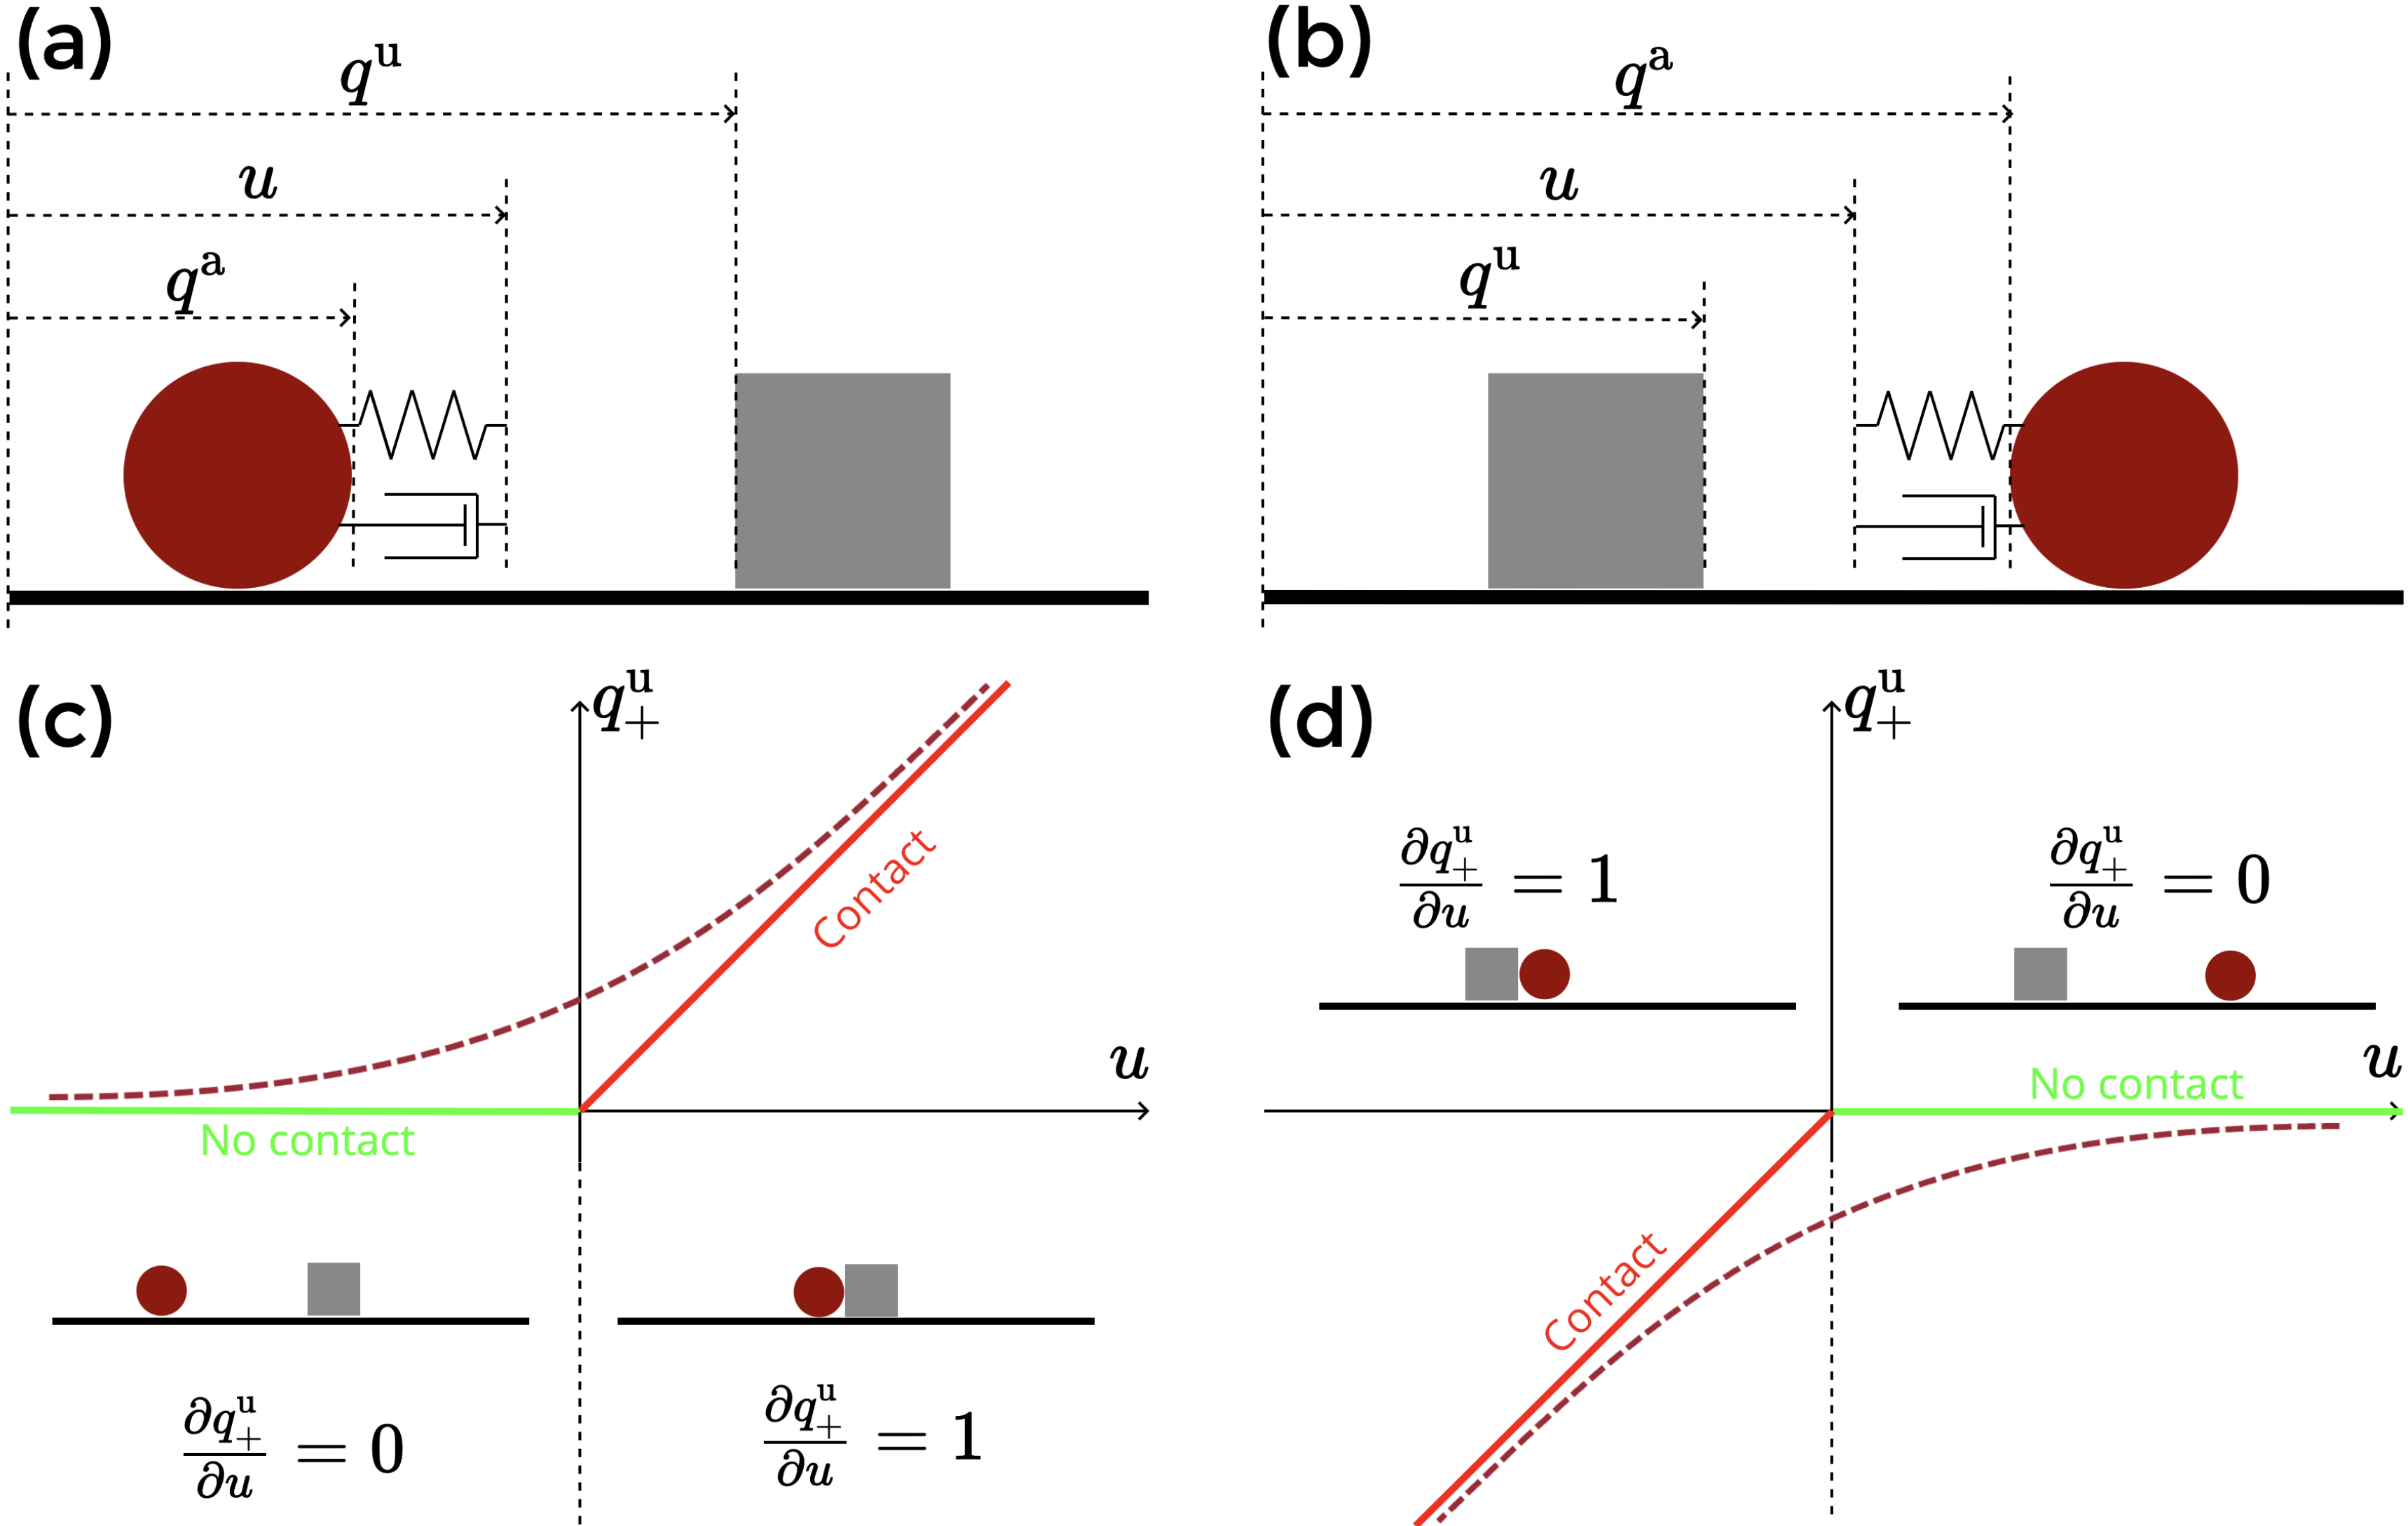
\includegraphics[width = 0.95\textwidth]{figures/01_intro/1d_box_ball.png}
\caption{(\textbf{a-b}) An actuated, PD-controlled ball and an un-actuated box, both are constrained to slide along a rail. (\textbf{a}): Ball on the left of the box. (\textbf{b}): Ball on the right of the box. (\textbf{c-d}) Dynamics of the ball-box system when the ball is on the (\textbf{c}) left or (\textbf{d}) right side of the box. Red and green indicate different contact modes. The maroon dashed lines are the smoothed contact dynamics after introducing the smoothing force field.}
\label{fig:intro:1d_box_ball}
\end{figure}

Starting from the system configuration in Fig. \ref{fig:intro:1d_box_ball}a,
let us consider the task of pushing the box to a goal configuration $q^\mathrm{u}_\text{goal}$ on the right of the box ($q^\mathrm{u}_\text{goal} > \qu$). To find an action $u$ that accomplishes the task, we can formulate an optimal control problem that penalizes the distance between the goal and the box position after the action $u$ is taken: % while respecting the \emph{dynamics} constraints imposed by the system:
\begin{equation}
\label{eq:intro:simple_task_objective}
\underset{u}{\mathrm{minimize}} \; \frac{1}{2}(q^\mathrm{u}_+ - q^\mathrm{u}_\text{goal})^2, %\text{subject to} \\
% & q^\mathrm{u}_+ = f(\qu, \qa, u),
\end{equation}
where $q^\mathrm{u}_+$ is the \emph{steady-state} position of the box after the ball is commanded to position $u$. Note that $q_+^\mathrm{u}$ depends on $\qu$, $\qa$ and $u$. For instance, if the ball starts on the left of the box ($\qa < \qu$, Fig. \ref{fig:intro:1d_box_ball}a), any $u$ to the left of the box ($u < \qu$) will not change the box's position, as the ball will not touch the box. In contrast, the box will follow the ball to the commanded $u$ when the ball makes contact with the box ($u \geq \qu$). 
The dependence of $q^\mathrm{u}_+$ on $(\qu, \qa, u)$ is commonly called the \emph{dynamics} of the system, and is plotted in Fig. \ref{fig:intro:1d_box_ball}c-d.

Gradient descent is a common way to minimize the cost \eqref{eq:intro:simple_task_objective}. Starting with an initial guess of $(\qu, \qa, u)$ (without loss of generality, we assume the ball is on the left of the box in the initial guess), gradient descent iteratively improves $u$ by taking steps opposite to the cost's gradient w.r.t. $u$:
\begin{equation}
\frac{\partial }{\partial u} \left(\frac{1}{2}(q^\mathrm{u}_+ - q^\mathrm{u}_\text{goal})^2\right)
= (q^\mathrm{u}_+ - q^\mathrm{u}_\text{goal}) \DfDx{q_+^\mathrm{u}}{u}.
\end{equation}

However, $\DfDx{q_+^\mathrm{u}}{u}$ is 0 unless the ball is touching the box, as shown in Fig. \ref{fig:intro:1d_box_ball}c-d. This means that if the box and ball are not in contact in the initial guess, the gradient $\DfDx{q_+^\mathrm{u}}{u}$ tells us nothing about how $u$ can be improved in order to get $q^\mathrm{u}_+$ closer to the goal $q^\mathrm{u}_\text{goal}$. 

To combat the zero gradient problem, we can \emph{smooth} the contact dynamics by introducing a force field between the box and the ball: the ball can push the box without touching it, and the magnitude of the force is inversely proportional to the distance between them. This force field will make $\DfDx{q_+^\mathrm{u}}{u}$ positive even when the box and ball are not touching (the dashed lines in Fig. \ref{fig:intro:1d_box_ball}c-d), thereby informing gradient descent the direction in which $u$ needs to be improved. To make sure that the actual non-smooth dynamics is satisfied at convergence, the amount of smoothing can be iteratively reduced during the gradient steps.

However, smoothing is not the panacea in contact-rich planning. For example, what if we want to push the box to the left ($q^\mathrm{u}_\text{goal} < \qu$), with an initial guess where the ball is also on the left of the box (Fig. \ref{fig:intro:1d_box_ball}a)? Following the gradient would move the ball further and further away from the box until $\DfDx{q_+^\mathrm{u}}{u}$ becomes so small that gradient descent converges. This is an example of gradient descent getting stuck in a bad local minimum. Bad local minima can be avoided to some extent with better initial guesses: in the box-ball system, starting gradient descent with the ball on the right of the box (as in Fig. \ref{fig:intro:1d_box_ball}b) would yield the correct $u$. However, for more complex problems, good initial guesses are rarely handed to us on a silver platter \cite{onol2020tuning }.

To avoid bad local minima without good initial guesses, we need a more \emph{global} search strategy that explores beyond the gradient (which greedily decreases the cost). A common way to organize the search is to divide the system dynamics into \emph{modes} based on which contacts are active. For the box-ball system, there are four modes: (i) left contact, (ii) left no contact, (iii) right contact and (iv) right no contact. Each mode corresponds to a linear piece in the dynamics (Fig. \ref{fig:intro:1d_box_ball}c-d), which is easy to analyze. In this case, the search for the optimal action $u$ can be done by solving \eqref{eq:intro:simple_task_objective} for every mode, and then picking the action with the lowest cost among all modes.

But the number of modes can grow out of control quickly. For a system with $n_\mathrm{c}$ rigid bodies, there are $\binom{n_c}{2}$ pairs of bodies, or \emph{contact pairs}, that can be in contact. Each contact pair can be in separation or in contact. If there is friction, ``in contact'' can be further divided into sticking, sliding left and sliding right, with even more sliding directions if the system is 3D. Other factors, such as the number of faces in a body, can also contribute the the number of modes. Although the four modes for the ball-box system seems manageable, the number of modes can be astronomical for more complex systems. For instance, the system in Fig. \ref{fig:intro:allegro_hand_and_melon}, consisting of a dexterous hand and a rigid object, has $6^{\binom{20}{2}} = 6^{190}$ contact modes \footnote{Each contact can be in separation, sticking or four directions of sliding ($6 = 1 + 1 + 4$). There are 20 bodies in the system.}. Although this number can be reduced into the trillions with a more efficient counting scheme such as \cite{huang2021efficient}, the reduced number of modes is still too much to handle for algorithms that reason explicitly about modes.

\begin{figure}
\centering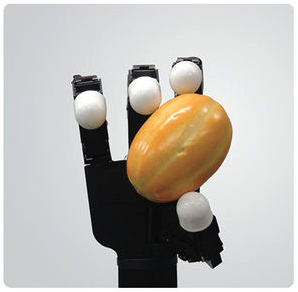
\includegraphics[width = 0.40\textwidth]{figures/01_intro/allegro_hand_and_melon.png}
\caption{The Allegro Hand and an oriental melon \cite{allegrohand}.}
\label{fig:intro:allegro_hand_and_melon}
% \vskip -0.25 true in
\end{figure}


\section{Related Work}
In Section \ref{sec:intro:box_ball_system}, we formulated a simple pushing task \eqref{eq:intro:simple_task_objective} as an optimal control problem \cite[\textsection 10]{underactuated}, and identified the non-smoothness in contact dynamics constraints as a key source of trouble in solving the problem. We have also illustrated the two major categories of model-based solutions towards the non-smoothness and their drawbacks: (\textbf{i}) nonlinear optimization using smoothed gradients of contact dynamics, which frequently get stuck in local minima, and (\textbf{ii}) considering contact mode transitions explicitly, which scales poorly due to the exponential explosion of the number of modes. 

In this subsection, after a brief review of how contacts are modeled numerically and how such modeling leads to non-smoothness, we will give a more detailed account on model-based contact-rich planning/control algorithms based on (\textbf{i}) nonlinear optimization and (\textbf{ii}) sequencing contact mode transitions. We will also discuss what model-based methods can learn from the success of applying RL to contact-rich manipulation, which has created the most impressive contact-rich manipulation demos (so far) on robotic hardware.


\subsection{Modeling Contact with Complementarity Constraints} 
\label{sec:intro:complementarity_constraints}
For a pair of rigid bodies, the contact force between them and the distance between them need to satisfy some intuitive constraints: (\textbf{i}) the contact force cannot push the bodies apart, (\textbf{ii}) the distance between the two bodies need to be non-negative, and (\textbf{iii}) non-zero contact force only exists when the two bodies are touching. 

Complementarity constraints are commonly used to mathematically represent the constraints above. In addition, the Coulomb friction law which governs the magnitude of friction forces, and the maximum dissipation principle which governs the direction of friction force during sliding, can also be represented with additional complementarity constraints \cite{stewart2000rigid, anitescu1997formulating}.

From a numerical optimization perspective, complementarity constraints are challenging to handle as they have no interior and violate constraint qualifications which are needed by gradient-based methods to converge \cite[\textsection 11]{biegler2010nonlinear}. As a result, in contact dynamics simulation, specialized algorithms such as pivoting methods or projected Gauss-Seidel \cite{SiggraphContact22} have been developed to efficiently handle the non-smoothness introduced by complementarity constraints. Instead of following the gradient of non-smooth constraints, these algorithms conduct a discrete search over which sides of the complementarity constraints are active: they start with a guess of the active sides and iteratively improves the guess until an iteration limit is reached, much like how the simplex algorithm searches for the optimal active set. Such algorithms are ideal if real-timeness is more important than physical accuracy, such as in video games: the algorithm can be terminated prematurely without satisfying all constraints. 

In contrast, contact-rich planning has different priorities: satisfaction of physics constraint is essential; and the planner has to look ahead more than one step (usually tens or even hundreds of steps) at a time. Therefore, a different set of techniques for handling complementarity constraints in the context of planning have been developed, and will be detailed in the next two sub-sections.

\subsection{Nonlinear Optimization}
\label{sec:intro:nonlinear_optimization}
An optimal control problem with contact dynamics constraints can be solved as a generic nonlinear program \cite{bertsekas1997nonlinear}. A typical gradient-based solution algorithm starts with an initial guess of the optimal trajectory, and iterates between (\textbf{i}) linearizing the cost and dynamics constraints around the current trajectory, (\textbf{ii}) updating the current trajectory in a direction that locally minimizes the cost \cite{gill2005snopt, todorov2005generalized}. 

As a consequence of the non-smoothness of contact dynamics, its linearization constructed from its gradient is no longer a good local approximation. Optimizing the cost locally with a bad understanding of the constraint landscape will lead to poor convergence behavior. 

Smoothing of contact constraints, therefore, has become an essential ingredient for good convergence when solving contact-rich planning problems. There are different ways in which smoothing can be introduced. Posa \textit{et al.}  and Manchester \textit{et al.} include the complementarity constraints directly as constraints of the optimal control problem. The complementarity constraints are relaxed to have non-empty interior \cite{posa2014direct, manchester2020variational}, thereby satisfying constraint qualifications \cite[\textsection 12]{nocedal1999numerical}. Tassa \textit{et al.} solve the optimal control problem with iterative LQR (iLQR), and imposes the dynamics constraints using rollouts \cite{tassa2012synthesis}. Their linearization of the dynamics is smoothed by regularizing the contact forces \cite{todorov2012mujoco}. Lastly, by penalizing constraint violation in the cost, Mordatch \textit{et al.} smooths contact constraints by not always strictly enforcing them and their associated non-smoothness \cite{mordatch2012contact}. Importantly, smoothing introduces some form of aphysical behavior into contact dynamics (such as the ``force-at-a-distance'' effect in Posa's relaxation \cite{posa2014direct} and Mujoco \cite{kolbert2016experimental}), and therefore needs to be iteratively decreased in order to respect the true dynamics constraint when the solution algorithm converges.

% My assessment: they scale well but get stuck in local minima.
By ``blending'' adjacent contact modes (e.g. Fig. \ref{fig:intro:1d_box_ball}c-d), smoothing extends the region where linearization is valid, thereby improving the performance of nonlinear optimization algorithms that rely heavily on linearization of dynamics constraints. With the help of smoothing, nonlinear optimization can find trajectories for complex systems such as humanoids on monkey bars \cite{dai2014whole}. However, nonlinear optimization frequently gets stuck in local minima due to the inherent non-convexity of many contact-rich planning problems, and thus requires non-trivial initial guesses.

\subsection{Contact Mode Transitions}
Another approach to handle the non-smoothness in contact dynamics is to ``chop up'' the dynamics into smooth pieces (contact modes). The ``chopping'' makes the dynamics within modes relatively straightforward, and shifts the difficulty of the planning problem to the transitions among modes. 

Mixed-Integer Programming (MIP) \cite{bertsimas1997introduction} naturally transcribes the smooth dynamics within modes and the discrete transitions between modes using continuous and integer variables, respectively \cite{marcucci2019mixed}. For simple systems (e.g. planar linear humanoid between walls \cite{marcucci2017approximate}), it is possible to discretize the entire state space and ask MIP solvers for a \emph{globally optimal} plan. Global MIP formulations of contact-rich planning problems, when solved, can yield trajectories that do not always greedily decrease the cost, making them difficult for nonlinear-optimization-based solvers to discover \cite{marcucci2019mixed}. 

Solving MIPs can be time-consuming and often too slow for using the planner at real-time rates as a Model-Predictive Controller (MPC). As a result, various techniques have been developed to accelerate solving MIPs in the context of contact-rich planning. Marcucci \textit{et al.} warm-start new MIPs using optimal solutions of similar problems \cite{marcucci2020warm}. Deits \textit{et al.} learned value functions for a humanoid push-recovery task, making MIPs smaller by reducing the planning horizon \cite{deits2019lvis}. Aydinoglu and Posa developed a specialized MIP solver which is based on the alternating direction method of multipliers (ADMM) and can solve small contact-rich planning problems at real-time rates \cite{aydinoglu2022real}. 

Despite these efforts to improve solver efficiency, discretizing the entire state space for even moderately large systems (e.g. pushing a box in a plane) will lead to too many contact modes for exiting methods find a solution within a reasonable amount of time (e.g. a couple of minutes). As a result, global optimality is usually given up in exchange for keeping the size of the planning problem manageable. For instance, considering only contact modes around a nominal trajectory instead of the entire state space can effectively reduce problem size \cite{hogan2020feedback, aceituno2020global}. However, by restricting the planner to search around a nominal trajectory, the ability to globally search the state space, a key feature to escape the local minima which plague methods based on nonlinear optimization, is lost. 

Is it possible to retain the ability of global search without incurring the cost of global mode enumeration? If we are willing to give up on global optimality, sampling contact modes, instead of enumerating them, is a good solution. Similar to classical Sampling-Based Motion Planning (SBMP) methods in the configuration space \cite{lavalle2006planning}, SBMP through contact builds a graph in the state space. From a node in the graph and its corresponding subgoal, the graph can be grown by randomly picking a contact mode and moving towards a subgoal as much as possible without causing a mode switch \cite{cheng2021contact, wu2020r3t}. 

SBMP with sampled mode transitions (e.g. \cite{cheng2021contact}) can handle moderately complex systems such as 3D peg-hole insertion with point fingers. It has the best scalability among all planning methods that consider mode transitions. However, the number of contact modes in more complex tasks, such as dexterous in-hand manipulation, will stagnate the search even if mode transitions are sampled instead of enumerated. This suggests that contact-rich manipulation planning may need a method that is fundamentally different from searching through mode switches.


\subsection{Reinforcement Learning}
Recent advances in deep RL have created impressive and convincing dexterous manipulation demos where a humanoid robotic hand in-hand re-orients a cube \cite{andrychowicz2020learning, handa2022dextreme}. A combination of domain randomization \cite{tobin2017domain} and Proximal Policy Optimization (PPO) \cite{schulman2017ppo}, the algorithm for training the policy is conceptually straightforward. Yet the complexity demonstrated in the learned policies far exceed the capabilities of the best model-based contact-rich planning methods. 

Although training an RL policy requires heavy offline computation, and the learned policy often lacks interpretability and the ability to generalize to new tasks, it is undeniable that RL has solved challenging problems with which model-based methods have struggled. Understanding the reasons behind RL's success from a model-based perspective will help us improve the performance of model-based methods. 

Recent works have attributed the success of RL to its stochastic nature, where the contact modes are abstracted by a process of sampling and averaging \cite{bundledgradients, pang2022global}. This process, termed ``randomized smoothing'', has a similar smoothing effect on contact dynamics as the various model-based smoothing schemes introduced in Sec. \ref{sec:intro:nonlinear_optimization}. Another key factor behind the empirical success of RL could lie in its goal of performing global optimization \cite{pang2022global}, which nonlinear optimization fails to do, and methods based on mode transitions can do only at limited scale.

This hints at a possible strategy of enhancing model-based contact-rich planning methods: if we could combine model-based smoothing with an efficient global search scheme, we might be able to achieve RL-level performance without incurring RL-level computational cost.


\section{Contributions and Thesis Structure}
Smoothing and global search are both essential to the success of contact-rich planning, but as far as we know, no existing method does both. This thesis proposes a contact-rich planning algorithm that searches globally under the guidance of a smoothed contact model. The proposed method can, within 1-minute of wall-clock time on a regular desktop computer, generate contact-rich plans for complex robotic systems such as dexterous hands.

At the heart of the model-based planning approach we took lies the question: what is the \emph{right} model for contact-rich manipulation? In Chapter \ref{chapter:quasi_static_dynamics}, we present a novel formulation of rigid-body contact dynamics that is quasi-static, convex, differentiable and amenable to smoothing, all of which are features chosen to improve the efficiency of the planner.

In Chapter \ref{chapter:contact_rich_planning}, we present the global contact-rich planner that utilizes the proposed quasi-static contact model and combines SBMP with trajectory optimization. Efficient global exploration is carried out with a kino-dynamic sampling-based motion planner that searches with large step sizes near the contact manifold. By abstracting contact modes away with a smoothed version of the contact dynamics, the sampling-based planner can effectively explore the state space without suffering from the exponential explosion of contact modes. Once a coarse path is found by the sampling-based planner, the path is refined by a trajectory optimizer with finer step sizes to improve its quality and physical accuracy. 

The challenges facing contact-rich manipulation extend far beyond planning. Once a plan is generated, interaction forces between the robot and the objects need to be sensed and estimated. The estimated forces, together with other estimated states, are then fed to a stabilizing controller that is aware of making and breaking contacts. 
Therefore, this thesis also explores (\textbf{i}) external contact force estimation from joint torque measurements (Chapter \ref{chapter:force_from_torque}), and (\textbf{ii}) reconciling tracking trajectory and bounding contact forces using a inverse-dynamics controller in the simple case of interacting with a static environment (Chapter \ref{chapter:quasi_static_control}). Interestingly, the methods in both Chapter \ref{chapter:force_from_torque} and \ref{chapter:quasi_static_control} benefit from the simplifying quasi-static assumption, highlighting the utility of quasi-static dynamics in various components of the robotic manipulation pipeline. 




\chapter{An Effective Contact Dynamics Model for Contact-rich Planning}
\label{chapter:quasi_static_dynamics}
\section{Introduction}
We believe an effective model for contact-rich manipulation planning needs to be 
(\textbf{i}) numerically robust
and (\textbf{ii}) differentiable, so that local linearizations can be reliably computed for planning. 
Most importantly, the model should be able to (\textbf{iii}) predict the \emph{long-term} behavior of the system, so that the planner can look far ahead while taking few steps.
Last but not least, the model should be (\textbf{iv}) amenable to smoothing in order to provide more informative locally linear models across contact modes. 

In this chapter, we present a contact dynamics model that satisfies all of the requirements above. Combining these ingredients enables our planner to reliably generate complex contact-rich plans that have so far been considered challenging for existing model-based approaches.

Specifically, we propose a \emph{convex} implicit time-stepping contact model (Sec. \ref{sec:convex_quasi_dynamic_contact_dynamics}). 
Among several existing schemes to convexify frictional contact constraints (Sec. \ref{sec:quasi_static_background}), we adopt Anitescu's convex relaxation \cite{anitescu2006optimization} which in practice only introduces mild non-physical behavior \cite{pang2021convex, castro2021unconstrained}. The convexity provides a clear numerical advantage over the traditional Linear Complementarity Problem (LCP) formulation \cite{anitescu1997formulating, stewart2000rigid}. Moreover, the derivatives of the dynamics with respect to the current state and control action can be readily computed using sensitivity analysis for convex conic programs \cite{agrawal2019differentiatingcone} (Sec. \ref{sec:quasi_dynamic_derivatives}). In addition, we will illustrate how Anitescu's convex relaxation compares to the LCP formulation, and why it introduces a non-physical ``boundary layer'' during sliding (Sec. \ref{sec:quasi_static:artifacts}).

For long-term predictability, we adopt the quasi-static assumption widely used in robotic manipulation \cite{mason2001mechanics, motioncones, aceituno2020global, cheng2021contact}. 
A quasi-static model ``sees'' further than its second-order counterpart by ignoring transient dynamics and focuses on transitions between steady-states. Furthermore, quasi-static models are simpler: not only do they have half as many states, they also do not need parameters to describe damping, as damping is modeled by throwing away kinetic energy at every time step.

In our quasi-static model, robots are modeled as an impedance source. However, throughout the long history of quasi-static models in robotic manipulation planning (Sec. \ref{sec:quasi_static_background}), robots have often been modeled as an admittance source. This can lead to an ill-defined behavior where the output cannot be uniquely determined by the input, thereby limiting the utility of quasi-static models in contact-rich planning. In Sec. \ref{sec:quasi_static:prescribed_motion_bad}, we will elaborate on the limitations of the admittance modeling choice, and how impedance can resolve these problems.

The proposed quasi-static model is validated by running the same input trajectories in a high-fidelity second-order simulator (Sec. \ref{sec:quasi_static:experiments}). Our results show that our model is able to approximate the second-order dynamics well if the system considered is highly damped and dominated by frictional forces. Furthermore, in contact-rich scenarios, our model can keep the simulation error small at larger step sizes than the second-order simulator.
 
Lastly, to leverage the benefits of smoothing (Sec. \ref{sec:smoothdynamics}) in contact-rich planning, we show that in addition to the standard randomized smoothing schemes (Sec. \ref{sec:randomizedmoothing}), our contact model can be smoothed out using a log-barrier relaxation (Sec. \ref{sec:analyticsmoothing}). In this relaxation scheme, the hard contact constraints are softly enforced by a log-barrier function, a common technique used in the interior-point method for convex programs \cite[\textsection 11]{boyd2004convex} \cite{howell2022dojo}.
We further show that the gradients of the smoothed contact model can be easily computed with the implicit function theorem.


\section{Background} \label{sec:q_dynamics:background}
In this section, we will review how quasi-static dynamical models have been applied in manipulation planning, and highlight the flaw of modeling robots as an admittance source (Sec. \ref{sec:quasi_static_background}). We will also discuss the features of and trade-offs between various convex relaxations of rigid-body contact models (Sec. \ref{sec:convex_contact_background}).

\subsection{Quasi-static Models in Robotic Manipulation} \label{sec:quasi_static_background}
Quasi-static models, which previous works have used extensively for robotic manipulation planning and control \cite{mason2001mechanics, motioncones, aceituno2020global, cheng2021contact, pang2021easing}, simplify Newtonian dynamics by removing terms related to velocity and acceleration, and focusing on contact forces at the core of robot-object interactions. Although the model cannot describe highly-dynamics behaviors such as spinning a pen between fingers \cite{mordatch2012contact}, it holds up for a wide variety of manipulation tasks, including many that involve dexterous hands \cite{andrychowicz2020learning}.

Quasi-static models also have a long history in robotic manipulation. Planar pushing is perhaps one of the earliest problems where quasi-static models are applied. Pioneering work by Mason and Lynch focuses on predicting the motion of an object supported on a horizontal surface without knowledge of the pressure distribution between the object and the surface \cite{mason1986mechanics, lynch1996stable}. Later work incorporates a detailed pressure distribution \cite{goyal1991planar, howe1996practical} and stochasticity \cite{zhou2017fast} into the quasi-static planar pushing model. Such models have been effectively employed in a Model Predictive Control (MPC) framework which enables an object pushed by a single point contact to track complex planar trajectories \cite{hogan2020feedback}. In addition to planar pushing, quasi-static models have also been applied in simple, planar instances of dexterous manipulation \cite{trinkle1993dexterous, pang1996complementarity}.

Halving the number of states by removing velocity is one of the most recognized advantages of quasi-static systems \cite[\textsection 10.1]{mason2001mechanics}.
However, by focusing on transitions between static equilibria and ignoring transients induced by damping and acceleration, a quasi-static model can look further into the future while taking fewer steps than its second-order counterpart, thereby reducing the planning horizon. 
We believe this temporal aspect of quasi-static models' advantage is important but often overlooked in the literature. In practice, many trajectory optimization formulations for manipulation enforce the second-order Newtonian dynamics \cite{landry2019differentiable, kurtz2022contact}. Although modeling the transients allows the discovery of more dynamic behaviors, we believe, especially in the manipulation setting, that the added computational complexity due to long planning horizon oftentimes outweighs the benefits. 

Despite their popularity, many popular variants of quasi-static models, such as \cite{mason1986mechanics, lynch1996stable, zhou2017fast, hogan2020feedback}, have a serious flaw: the next state cannot be always be uniquely determined from the current state and control input.
In quasi-static models, the control input is usually defined as the position commands of the robots. 
Many quasi-static models also assume that the position commands can be perfectly executed as prescribed robot motions. Under this assumption, contact forces and object motions can be ambiguous for the same control input. This flaw does not manifest in simple tasks such as planar pushing, where robot motion does uniquely determine object motion. On the other hand, it can be crippling in more complex tasks such as grasping (more details in Sec. \ref{sec:quasi_static:prescribed_motion_bad}). 

It is possible to circumvent the ambiguity by including contact forces as additional states of the dynamics model \cite{trinkle1993dexterous, aydinoglu2020contact}. However, reasoning about both positions and forces compels the planner to handle the complementarity constraints between forces and distances, thereby limiting the algorithms the planner can employ.

A more fundamental remedy to this flaw is to account for the unmodeled compliance in the system, thereby allowing commanded and actual robot positions to be different. For instance, Harm and Posa added compliance at the robot joints by modeling the robot as velocity-controlled with finite gains \cite{halm2018quasi}; in previous work we added compliance at the contact points \cite{pang2018robust}. However, these remedies do not always reflect the reality on robotic hardware, which often consists of rigid objects and impedance-controlled robots. Moreover, \cite{pang2018robust} is too computationally expensive, and \cite{halm2018quasi} is developed specifically for manipulating planar objects supported on a tabletop.

In Sec. \ref{sec:quasi_static:prescribed_motion_bad}, we will discuss in more detail the flaws of commanding prescribed robot motions, and how our quasi-static formulation resolves it in a computationally-efficient and hardware-consistent manner. 


\subsection{Convex Rigid-body Contact Dynamics} \label{sec:convex_contact_background}
Without friction, quasi-static dynamics with frictionless unilateral contacts can be written as the KKT optimality conditions of a convex Quadratic Program (QP) that minimizes the system's potential energy subject to non-penetration constraints \cite{pang2021convex}. The complementarity between forces and distances (Sec \ref{sec:intro:complementarity_constraints}) are captured by the complementarity slackness between primal constraints and dual variables. However, the Coulomb friction law and the maximum dissipation principle, both of which are needed to model frictional contacts, introduce additional complementarity constraints that can no longer be accommodated by a convex program. Consequently, contact dynamics with Coulomb friction is formulated as an LCP, which is solved by specialized non-convex solvers \cite{anitescu1997formulating, stewart2000rigid}.

Anitescu restored convexity in contact dynamics by replacing the linear complementarity constraints with cone complementarity constraints. The price of convexity is that the sliding velocity is no longer restricted to the tangent plane defined by the contact normal \cite{anitescu2006optimization, SiggraphContact22}. The resulting program is a convex QP with discretized friction cones, or a Second-Order Cone Program (SOCP) with circular friction cones. Both formulations can be readily solved with commercial convex solvers such as \cite{mosek}.

Anitescu's convex relaxation exactly reproduces Coulomb friction when the contact is sticking, and injects a non-physical ``boundary layer'' between relatively-sliding objects. A big advantage of Anitescu's relaxation is that the extent of relaxation is controlled by only one hyperparameter: the step size. As the step size converges to 0, the boundary layer also vanishes \cite{anitescu2006optimization}. The step size therefore can serve as a knob that allows the planner to trade the dynamics model's predictive power for physical accuracy. We will discuss this non-physical behavior in more detail in Sec. \ref{sec:quasi_static:artifacts}.

The popular MuJoCo simulator\cite{todorov2012mujoco, todorov2014convex} solves a convex program that closely resembles the dual of Anitescu's formulation \cite[Appendix B]{underactuated}. Moreover, Mujoco also adds regularization on contact forces to the objective function in order to improve numerical conditioning and make the dynamics invertible. However, the regularization introduces non-physical behaviors such as ``force at a distance'' that are harder to control as they are induced by many hyper-parameters \cite{kolbert2016experimental}. 

Recently, Castro \textit{et al.} developed an unconstrained convex formulation of contact dynamics \cite{castro2021unconstrained} that combines many of the nice features from MuJoCo \cite{todorov2012mujoco} and Anitescu's convex relaxation \cite{anitescu2006optimization}. For instance, Castro's primal formulation is similar to Anitescu's; the contact force regularization and the removal of friction cone constraints using a projection function are inspired by similar techniques from MuJoCo. 
Castro's formulation is designed from ground up for efficient and accurate physics simulation. For instance, it provides physical interpretations and units to the contact force regularization parameters that are originally proposed by MuJoCo to improve numerical conditioning.
% Similar to MuJoCo, Castro's unconstrained formulation has regularization on contact forces. However, Castro proposed a rigorous methodology for setting the regularization in a way that respects simulation accuracy. 


\section{A Convex, Quasi-static and Differentiable Contact Model} \label{sec:q_dynamics:cqdc}
In this section, we present the Convex, Quasi-static, Differentiable Contact (CQDC) model which will be used for the contact-rich planning tasks in Chapter \ref{chapter:contact_rich_planning}. Specifically, we will start with the equations of motion of quasi-static contact dynamics, and massage it into the KKT optimality conditions of a convex optimization program (Sec. \ref{sec:convex_quasi_dynamic_contact_dynamics}). We will then describe how to take the (discontinuous) derivatives of the proposed contact dynamics (Sec. \ref{sec:quasi_dynamic_derivatives}), and how the forward dynamics and gradient computation are implemented (Sec. \ref{sec:quasi_static:implementation}). In addition, we will illustrate how Anitescu's convex relaxation introduces a non-physical ``boundary layer'' during sliding (Sec. \ref{sec:quasi_static:artifacts}). We will also dive more deeply into the common flaw in quasi-static dynamical models brought up in Sec. \ref{sec:q_dynamics:background}, and explain how our quasi-static model resolves it (Sec. \ref{sec:quasi_static:prescribed_motion_bad}). Lastly, with two examples of common manipulation tasks, we show that the proposed quasi-static model and an established second-order simulator (Drake \cite{drake}) generate very similar state trajectories for the same action sequence (Sec. \ref{sec:quasi_static:experiments}). 

\subsection{Forward Dynamics} \label{sec:convex_quasi_dynamic_contact_dynamics}
Despite the numerical advantage of convex contact dynamics formulations \cite{anitescu2006optimization, todorov2012mujoco, castro2021unconstrained}, some formulations can produce highly inaccurate contact forces with poorly-chosen hyperparameters \cite{kolbert2016experimental}. Our formulation adopts Anitescu's convex relaxation of the Coulomb friction constraints \cite{anitescu2006optimization}. Anitescu's convex relaxation is equivalent to common LCP formulations \cite{stewart2000rigid} in non-sliding contacts or in separation, and introduces a non-physical yet mild ``boundary layer'' effect between relatively-sliding objects \cite{pang2021convex, castro2021unconstrained}. Not only does Anitescu's convex friction model have the simulation step size $h$ as the only hyperparameter, the ``boundary layer'' also disappears as $h \rightarrow 0$. The step size therefore can serve as a knob that allows the planner to trade the dynamics model's predictive power for physical accuracy.

A generic discrete-time dynamical system is written as
\begin{equation}
\label{eq:f_x_u}
x_+ = f(x, u) 
\end{equation}
where $x \in \mathbb{R}^n$ is the state, $u \in \mathbb{R}^m$ the control input, and $f: \mathbb{R}^n\times\mathbb{R}^m\rightarrow\mathbb{R}^n$ the system dynamics. 
In the robotic manipulation setting, a system can be divided into $\nA$ \emph{actuated} Degree of Freedoms (DOFs), which correspond to the robots, and $\nU$ \emph{unactuated} DOFs, which correspond to the objects. The configurations of objects and robots are denoted respectively by $\qu \in \R[\nU]$ and $\qa \in \R[\nA]$. The system state is defined by $x \coloneqq q \coloneqq (\qu, \qa)$. We model the robots as impedances \cite{hogan1985impedance}, which in the quasi-static setting reduces to springs with a diagonal stiffness matrix $\Ka \in \R[\nA \times \nA]$. Accordingly, the input $u \in \R[\nA]$ is defined by the commanded positions of the robots' joints, which can also be interpreted as the equilibrium positions of the springs.

The discretized quasi-static equations of motion are
\begin{subequations}
\label{eq:q_dynamics_eom}
\begin{align} 
h \Ka \left(\qa + \dqa - u \right) &= h\tauA + \sum_{i=1}^{\nC} (\Ja[i])^\intercal \lambda_i, \label{eq:q_dynamics_eom:a}\\
\left( \frac{\epsilon}{h} \Mu \right) \dqu &= h\tauU + \sum_{i=1}^{\nC} (\Ju[i])^\intercal \lambda_i, \label{eq:q_dynamics_eom:u}
\end{align}
\end{subequations}
where $h \in \R_{++}$ is the step size in seconds; $\Mu \in \R[\nU \times \nU]$ is the mass matrix of the objects; $\epsilon \in \R_{+}$ is a small regularization constant; the change in system configuration from the current to the next step is $\dq \coloneqq (\dqu, \dqa)$; $\tauA \in \R[\nA]$ and $\tauU \in \R[\nU]$ are non-contact external torques (e.g. due to gravity) for robots and objects. There are $\nC$ contact pairs at the current time step. For the $i$-th contact, $\lambda_i \in \R[3]$ is the contact impulse; $\Ja[i] \in \R[3 \times \nA]$ and $\Ju[i] \in \R[3 \times \nU]$ are the contact Jacobians \cite{anitescu1996formulating} of the robots and the objects, respectively. For 3D systems, it is common that the rotational displacement and the angular velocity are different and related by a linear map. As the technique to deal with this difference is standard (e.g. \cite[Section II]{castro2021unconstrained}), we leave it out here for brevity and notational simplicity.

Equation \eqref{eq:q_dynamics_eom:a} states that the robot joint positions' deviation from their commanded values $u$, as a result of external impulses, is proportional to the stiffness $\Ka$. 
Equation \eqref{eq:q_dynamics_eom:u} can have different physical interpretations depending on the value of the regularization constant $\epsilon$.
If $\epsilon = 0$, \eqref{eq:q_dynamics_eom:u} is the force (impulse) balance of the objects. This corresponds to the exact quasi-static formulation in  \cite{pang2021convex}. 
If $\epsilon = 1$, \eqref{eq:q_dynamics_eom:u} is the standard second-order rigid body equations of motion (expressed in impulse-momentum form) for a system with 0 velocity at the current time step. 
This corresponds to Mason's classical definition of quasi-dynamic systems \cite{mason2001mechanics}. 
Note that for any $\epsilon$, the momentum gained at every step due to external impulses is discarded at the next time step, which is characteristic of the highly damped behavior typical in quasi-static systems.

In our physical experiments in later sections where objects are light, we find that the dynamics is closer to being exactly quasi-static ($\epsilon = 0$) than being classically quasi-dynamic ($\epsilon = 1$). Therefore, we pick $\epsilon$ to be as small as possible without causing numerical issues. A rule of thumb is to set $\epsilon$ such that the largest eigenvalue of $(\epsilon \Mu / h)$ is one tenth of the smallest eigenvalue of $(h \Ka)$ (see the definition of $\mathbf{Q}$ in \eqref{eq:q_dynamic_socp:Q_and_b}).
% $\epsilon$ needs to be set based on how much damping forces the robot experiences as it interacts with the object.

In addition, the Coulomb friction model requires the contact impulses $\lambda_i$ to stay inside the friction cone, and the relative sliding velocities to satisfy the maximum dissipation principle \cite{stewart2000rigid}. To enforce these constraints, we first introduce some additional notation. The contact Jacobian for contact $i$ is 
\begin{equation}
\label{eq:contact_jacobian_i}
\J_i \coloneqq [\Ju[i], \Ja[i]] \coloneqq 
\begin{bmatrix}
\Jn[i] \\
\Jt[i]
\end{bmatrix}
\in \R[3 \times (\nU + \nA)],
\end{equation}
where $\Jn[i] \in \R[1 \times (\nU + \nA)]$ maps the generalized velocity of the system to the normal contact velocity, and $\Jt[i] \in \R[2 \times (\nU + \nA)]$ to the tangent velocities. Next, the friction cone at contact $i$, $\mathcal{K}_i$, and its dual cone $\mathcal{K}_i^\star$, are denoted by
\begin{subequations}
\label{eq:contact_cones}
\begin{align}
\mathcal{K}_i &\coloneqq \left\{\lambda_i = (\lambda_{\mathrm{n}_i}, \lambda_{\mathrm{t}_i}) \in \R[3] | \mu_i \lambda_{\mathrm{n}_i} \geq \sqrt{\lambda_{\mathrm{t}_i}^\intercal \lambda_{\mathrm{t}_i}} \right\}, \label{eq:contact_cones:lambda}\\
\mathcal{K}_i^\star &\coloneqq \left\{v_i = (v_{\mathrm{n}_i}, v_{\mathrm{t}_i}) \in \R[3] | v_{\mathrm{n}_i} \geq \mu_i \sqrt{v_{\mathrm{t}_i}^\intercal v_{\mathrm{t}_i}} \right\}, \label{eq:contact_cones:v}
\end{align}
\end{subequations}
where $\mu_i$ is the friction coefficient; the dual variable $v_i$ can also be interpreted as the relative contact velocity for contact $i$; the subscripts $(\cdot)_\mathrm{n}$ and $(\cdot)_\mathrm{t}$ indicate respectively the normal and tangential components. 

With this notation, Anitescu's frictional contact constraints can be written as:
\begin{subequations}
\label{eq:friction_constraints}
\begin{align}
v_i \coloneqq 
\J_i
{\delta q}
+
\begin{bmatrix}
\phi_i \\
0_2
\end{bmatrix}
&\in \mathcal{K}_i^\star, \label{eq:friction_constraints:v_i}\\
\lambda_i &\in \mathcal{K}_i, \\
v_i^\intercal \lambda_i &= 0, \label{eq:friction_constraints:complementary_slackness}
\end{align}
\end{subequations}
where $\phi_i \in \R$ is the signed distance for contact $i$ at the current time step. These constraints enforce the Coulomb friction model exactly when a contact is sticking (not sliding) and in separation. In sliding, these constraints enforce maximum dissipation, but adds a small gap between the two relatively-sliding objects. Anitescu showed that this gap converges to 0 as $h \rightarrow 0$ \cite{anitescu2006optimization}.

Remarkably, this implies that the quasi-static equations of motion \eqref{eq:q_dynamics_eom}, together with the friction constraints \eqref{eq:friction_constraints}, are the KKT optimality conditions \cite[\textsection 5.9]{boyd2004convex} of the following convex Second-Order Cone Program (SOCP) \cite{anitescu2006optimization}:
\begin{subequations}
\label{eq:q_dynamic_socp}
\begin{align}
&\underset{\dq}{\minimize} \; \frac{1}{2} \dq^\intercal \mathbf{Q} \dq + b^\intercal \dq, \; \text{subject to} \label{eq:q_dynamic_socp:cost}\\
&\qquad \qquad \J_i
{\delta q}
+
\begin{bmatrix}
\phi_i \\
0_2
\end{bmatrix}
\in \mathcal{K}_i^\star, \; \forall i \in \{1 \dots \nC\}, \; \text{where} \label{eq:q_dynamic_socp:constraint}\\
&\mathbf{Q} \coloneqq \begin{bmatrix} \epsilon \Mu/h & 0 \\ 0 & h \Ka \end{bmatrix}, \;
b \coloneqq - h\begin{bmatrix} \tauU \\ \Ka(u - \qa) + \tauA \end{bmatrix}, \label{eq:q_dynamic_socp:Q_and_b}
\end{align}
\end{subequations}
whose primal and dual solutions, $\dq^\star$ and $\lambda^\star \coloneqq (\lambda_1^\star, \dots, \lambda_{\nC}^\star)$, can be obtained by conic solvers such as \cite{mosek, scs}. Note that when $\epsilon=0$, which corresponds to strictly enforcing force balance on the object, the objective \eqref{eq:q_dynamic_socp:cost} is positive semi-definite, and thus \eqref{eq:q_dynamic_socp} may have multiple solutions.  

The SOCP \eqref{eq:q_dynamic_socp} reduces to a QP when there is no friction or if the friction cone can be described by linear constraints. The second-order friction cones \eqref{eq:contact_cones} can be equivalently represented as linear constraints in the planar case, or be approximated with polyhedral cones \cite{stewart2000rigid} in the 3D case. However, this approximation introduces non-physical anisotropic behaviors \cite{li2018implicit, howell2022dojo}, which is why \eqref{eq:contact_cones} is preferred.

\subsection{Differentiability} \label{sec:quasi_dynamic_derivatives}
We illustrate how to compute the derivatives of the system configuration at the next step, $q_+$, with respect to the current $q$ and $u$. Let us express the forward contact dynamics in the standard dynamical system form \eqref{eq:f_x_u}:
\begin{equation}
\label{eq:f_q_u}
q_+ = f(q, u) = q + \dq^\star(q, u),
\end{equation}
where $\dq^\star$ is the solution to  \eqref{eq:q_dynamic_socp}. Taking the derivatives of \eqref{eq:f_q_u} yields
\begin{equation}
\label{eq:q_dynamics_AB}
\A = \DfDx{f}{q} = \I + \DfDx{\dq^\star}{q}, \;
\B = \DfDx{f}{u} = \DfDx{\dq^\star}{u},
\end{equation}
where $\DfDxLine{\dq^\star}{q}$ and $\DfDxLine{\dq^\star}{u}$ can be expanded using the chain rule into:
\begin{subequations}
\label{eq:dq_star_q_u}
\begin{align}
\DfDx{\dq^\star}{q} &= \DfDx{\dq^\star}{b} \DfDx{b}{q} + \DfDx{\dq^\star}{\mathbf{Q}}\DfDx{\mathbf{Q}}{q} + \sum_{i=1}^{\nC} \DfDx{\dq^\star}{\J_i}\DfDx{\J_i}{q} + \DfDx{\dq^\star}{\phi_i}\DfDx{\phi_i}{q}, \label{eq:DdqDq}\\
\DfDx{\dq^\star}{u} &= \DfDx{\dq^\star}{b} \DfDx{b}{u}. \label{eq:DdqDu}
\end{align}
\end{subequations}

Similar to other differentiable simulators based on implicit time-stepping \cite{werling2021fast, howell2022dojo}, we compute the derivatives of the solution $\dq^\star$ with respect to the problem data $(\mathbf{Q}, b, \J_i, \phi_i)$ by applying the implicit function theorem to the KKT optimality conditions of the convex program \eqref{eq:q_dynamic_socp} \cite{agrawal2019differentiatingcone}. 
Then, the derivatives of $(\mathbf{Q}, b, \J_i, \phi_i)$ with respect to $q$ and $u$ can be straightforwardly computed using either automatic differentiation or a more specialized method that takes advantage of the structure of rigid body systems \cite{carpentier2018analytical}.

As the derivatives \eqref{eq:dq_star_q_u} are discontinuous functions of $(q, u)$ \cite{bundledgradients}, they are not a good local approximation of the CQDC dynamics unless multiple gradients are computed for different state-action pairs and averaged using the first-order randomized smoothing scheme (Sec. \ref{sec:smoothdynamics}).

\subsection{Implementation} \label{sec:quasi_static:implementation}
As all existing rigid-body differentiable simulators, to the best of our knowledge, assume second-order Newtonian dynamics, it is difficult and inefficient to modify them to support our CQDC dynamics formulation. Therefore, we implemented the proposed dynamics formulation using the Drake robotics toolbox \cite{drake}. Although our implementation is not heavily optimized, it is adequate for computing contact-rich plans within a reasonable amount of wall-clock time (a few minutes). 

For the forward dynamics (Sec. \ref{sec:convex_quasi_dynamic_contact_dynamics}), we use Drake's \code{MultibodyPlant} and \code{SceneGraph} for collision detection and the computation of the object mass matrix $\Mu$, contact Jacobians $\J_i$ and signed distances $\phi_i$. The SOCP \eqref{eq:q_dynamic_socp} can then be constructed with \code{MathematicalProgram} and solved with a third-party solver of our choice.

For the dynamics derivatives (Sec. \ref{sec:quasi_dynamic_derivatives}), we have a custom implementation for differentiating through the KKT optimality conditions of an SOCP using Eigen's \cite{eigenweb} linear solvers, allowing us to efficiently compute the partial derivatives of $\dq^\star$ with respect to $(\mathbf{Q}, b, \J_i, \phi_i)$ from primal-dual solutions $(\dq^\star, \lambda^\star)$ given by third-party conic solvers. As for the partials of $(\mathbf{Q}, b, \J_i, \phi_i)$ with respect to $q$, we note that $b$ is a linear function of $q$;  $\DfDxLine{\phi_i}{q} = \Jn[i]$; $\DfDxLine{\J_i}{q}$ and $\DfDxLine{\mathbf{Q}}{q}$ are computed with Drake's forward-mode automatic differentiation.

Finally, in order to avoid discontinuities coming from collision detection, we curate our system models so that every contact pair is either sphere-sphere, sphere-box, or sphere-cylinder, which means the contact points and normals change smoothly with the system configuration $q$ \cite{SiggraphContact22}. For example, in Fig. \ref{fig:rrt_tasks}, both the box-shaped fingers of the Allegro hand and the box-shaped manipuland in the Allegro Plate system are represented as arrays of inscribing spheres for the purpose of collision detection.
We note that this limitation can be alleviated with smoothing over collision geometries \cite{simonsinglelevel,randomizedsmoothingcollision}. 

\subsection{Interpreting Anitescu's Convex Relaxation} \label{sec:quasi_static:artifacts}
In this subsection, we will explain for planar (2D) systems how complementarity constraints in Anitescu's relaxation behave in different contact modes, namely sticking, sliding and separation. We will also illustrate the cause of the ``boundary layer'' artifact during sliding.

When both robots and objects are constrained in a plane, the CQDC dynamics \eqref{eq:q_dynamic_socp} simplifies to the following QP:
\begin{subequations}
\label{eq:q_dynamics_planar_qp}
\begin{align}
\underset{\dq}{\minimize} \; &\frac{1}{2} \dq^\intercal \mathbf{Q} \dq + b^\intercal \dq, \; \text{subject to} \\
&(\Jn[i] + \mu_i \Jt[i]) \dq + \phi_i \geq 0, \; i \in \{1\dots\nC\}, \label{eq:q_dynamics_planar_qp:constraint1}\\
&(\Jn[i] - \mu_i \Jt[i]) \dq + \phi_i \geq 0, \; i \in \{1\dots\nC\}, \label{eq:q_dynamics_planar_qp:constraint2}
\end{align}
\end{subequations}
where the contact Jacobian $\Jt[i]$ has only one row instead of two, and the conic contact constraint \eqref{eq:q_dynamic_socp:constraint} reduces to two inequality constraints \eqref{eq:q_dynamics_planar_qp:constraint1} and \eqref{eq:q_dynamics_planar_qp:constraint2}. The KKT conditions of \eqref{eq:q_dynamics_planar_qp} include the following complementarity constraints for the $i$-th contact pair:
\begin{subequations}
\label{eq:anitescu_friction_single_contact}
\begin{align}
0 \leq \beta_{i1} &\perp  (\Jn[i] + \mu_i \Jt[i]) \dq + \phi_i \geq 0, \label{eq:anitescu_friction_single_contact:a}\\
0 \leq \beta_{i2} &\perp  (\Jn[i] - \mu_i \Jt[i]) \dq + \phi_i \geq 0, \label{eq:anitescu_friction_single_contact:b}
\end{align}
\end{subequations}
where the Lagrange multipliers $\beta_{i1}$ and $\beta_{i2}$ are no longer the normal and tangential component of the contact impulses. Instead, they are the components of the contact impulses along the extreme rays of the friction cone (Fig. \ref{fig:anitescu_constraints_detailed}a). 

As the interplay between contact impulses ($\beta_{i1}, \beta_{i2}$) and non-penetration constraints (RHS of \eqref{eq:anitescu_friction_single_contact}) are best shown in the contact frame of contact pair $i$, we define the relative Cartesian translation of contact pair $i$ during the time step as $\delta \mathsf{x}_i \coloneqq [\delta \mathsf{n}_i, \delta \mathsf{t}_i] \in \mathbb{R}^2$, where $\delta \mathsf{n}_i \coloneqq \Jn[i] \dq \in \mathbb{R}$ and $\delta \mathsf{t}_i \coloneqq \Jt[i] \dq \in \mathbb{R}$ are the normal and tangential components of $\delta \mathsf{x}_i$ respectively. These quantities are illustrated in Fig. \ref{fig:anitescu_constraints_detailed}c. With this notation, \eqref{eq:anitescu_friction_single_contact} can be written as
\begin{subequations}
\label{eq:anitescu_friction_single_contact_alt}
\begin{align}
0 \leq \beta_{i1} &\perp \delta \mathsf{n}_i + \mu_i \delta \mathsf{t}_i + \phi_i  \geq 0, \label{eq:anitescu_friction_single_contact_alt:a}\\
0 \leq \beta_{i2} &\perp  \delta \mathsf{n}_i - \mu_i \delta \mathsf{t}_i + \phi_i \geq 0. \label{eq:anitescu_friction_single_contact_alt:b}
\end{align}
\end{subequations}


Note that (\textbf{i}) the feasible region of $\delta \mathsf{x}_i$ is defined by the RHS of (\ref{eq:anitescu_friction_single_contact_alt:a}) and (\ref{eq:anitescu_friction_single_contact_alt:b}); (\textbf{ii}) both boundaries of the feasible region of $\delta \mathsf{x}_i$ (the blue and red dashed lines in Fig. \ref{fig:anitescu_constraints_detailed}) intersect the $\mathsf{n}_i$-axis at $-\phi_i$, which is non-positive; (\textbf{iii}) the normal and tangential contact force impulses are given respectively by $\lambda_{\mathrm{n}_i} = \beta_{i1} + \beta_{i2}$ and $\lambda_{\mathrm{t}_{i}} = \mu_i \left( \beta_{i1} - \beta_{i2}\right)$.

\begin{figure}[ht!]
\centering
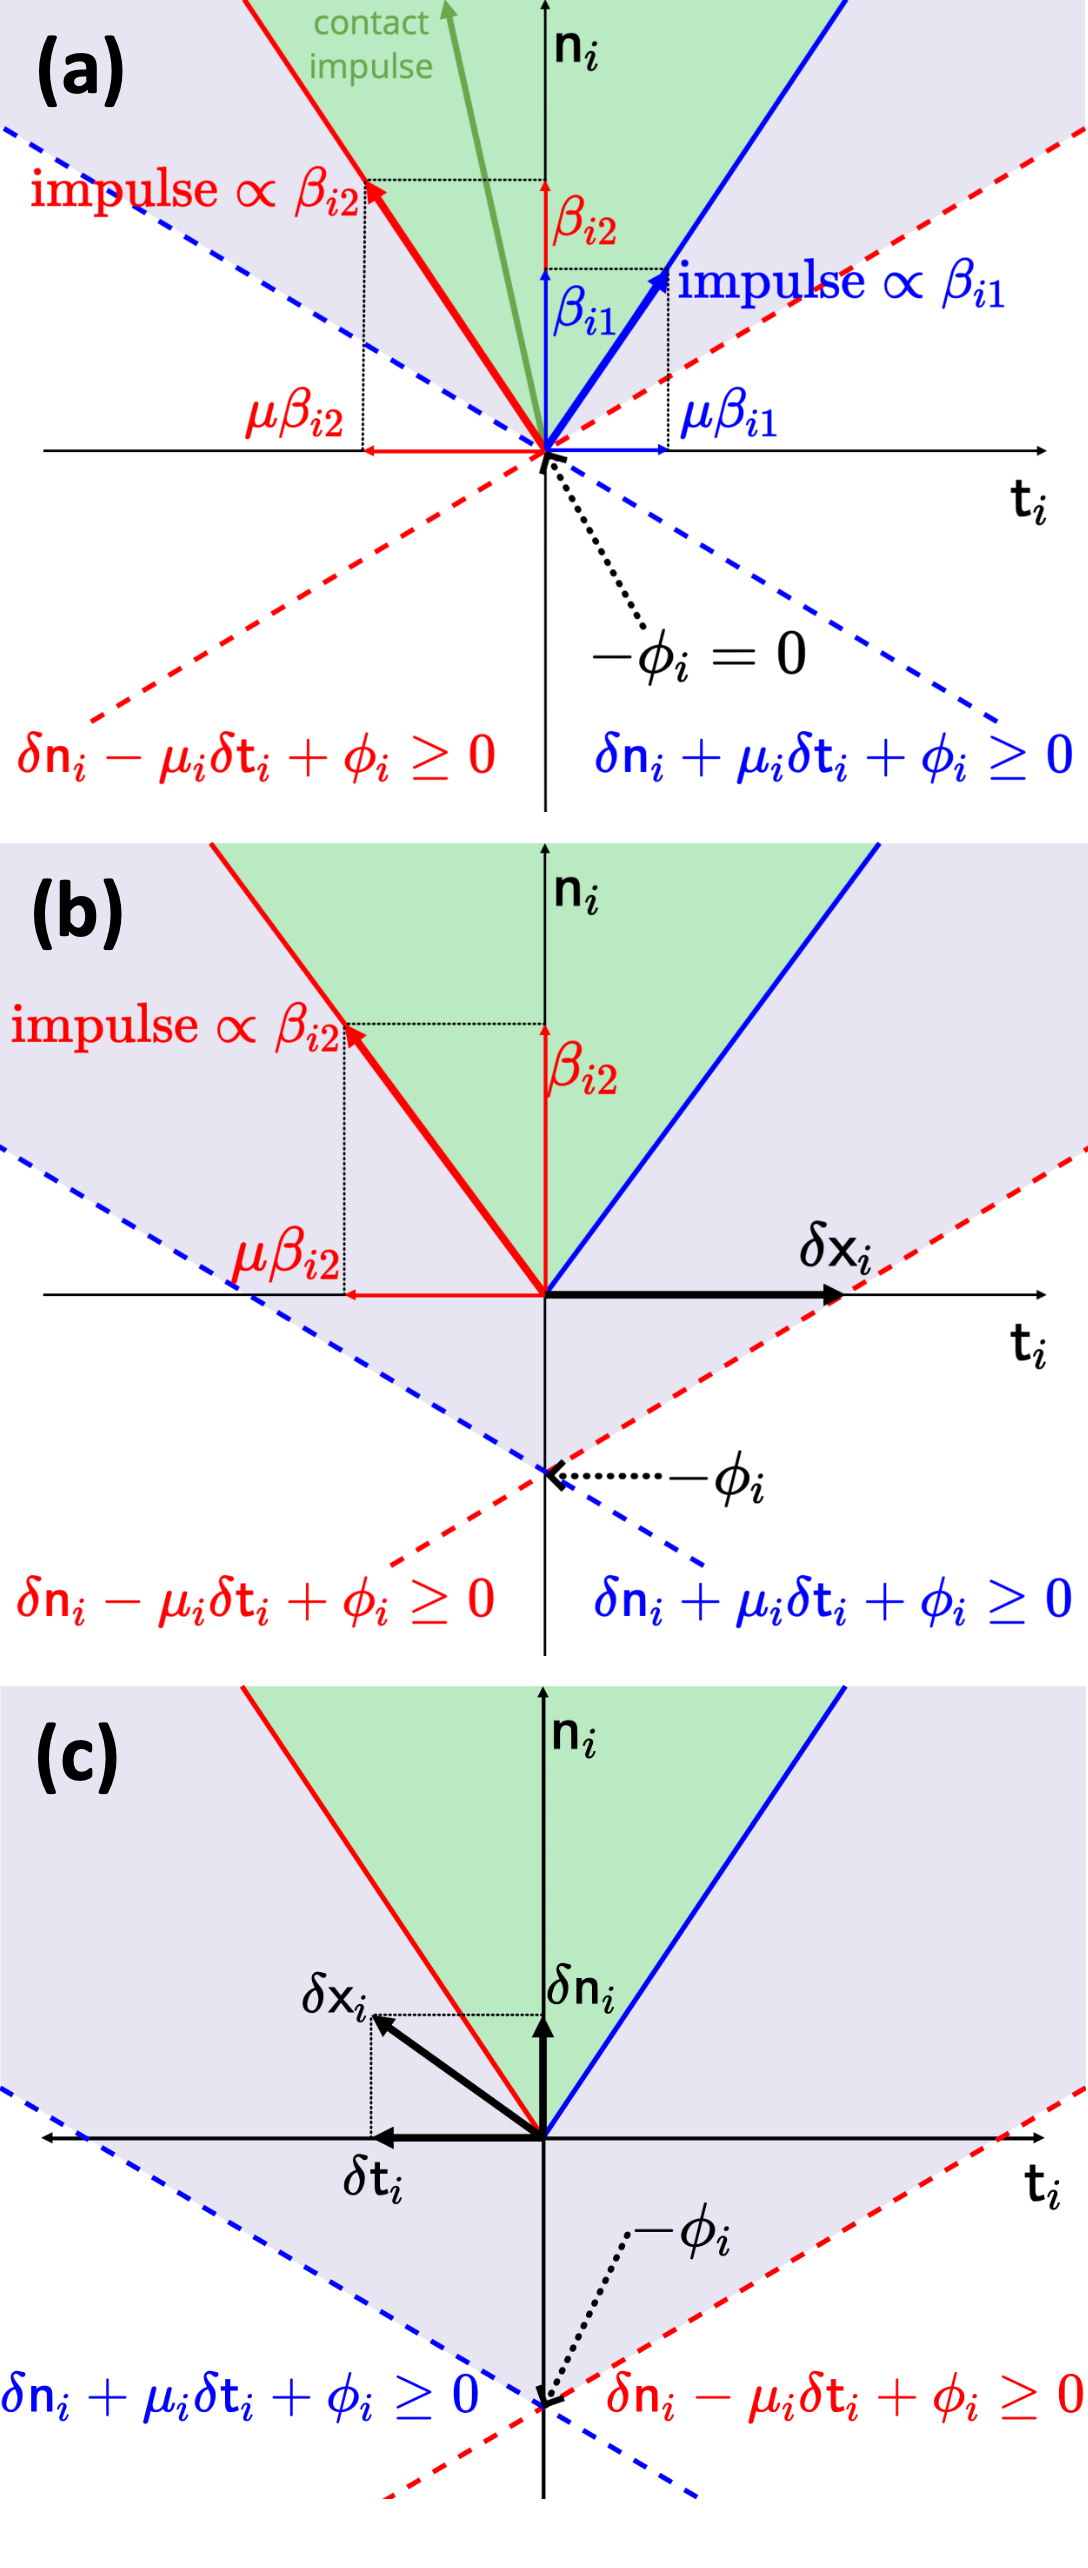
\includegraphics[width=0.53\linewidth]{figures/02_quasi_static_dynamics/anitescu_constraints_detailed.png}
\caption{Anitescu's friction constraints (\ref{eq:anitescu_friction_single_contact_alt}) under different contact modes: (\textbf{a}) sticking, (\textbf{b}) sliding, and (\textbf{c}) separation. The normal and tangent of the contact frame $i$ are denoted respectively by $\mathsf{n}_i$ and $\mathsf{t}_i$. The green shaded area is the friction cone. The purple shaded area is the feasible region of $\delta \mathsf{x}_i$. Constraints corresponding to (\ref{eq:anitescu_friction_single_contact_alt:a}) and (\ref{eq:anitescu_friction_single_contact_alt:b}) are color-coded blue and red, respectively.}
\label{fig:anitescu_constraints_detailed}
\end{figure}

\subsubsection{Sticking (Fig. \ref{fig:anitescu_constraints_detailed}a)} In a sticking contact, $\delta \mathsf{x}_i= 0$, $\phi_i = 0$ and the contact force is inside the friction cone. The conditions for sticking, $\delta \mathsf{x}_i= 0$ and $\phi_i = 0$, imply that $ \delta \mathsf{n}_i + \mu_i \delta \mathsf{t}_i + \phi_i = 0$ and $\delta \mathsf{n}_i - \mu_i \delta \mathsf{t}_i + \phi_i = 0$, i.e. the RHS of (\ref{eq:anitescu_friction_single_contact_alt:a}) and (\ref{eq:anitescu_friction_single_contact_alt:b}) are active. Therefore, both $\beta_{1i}$ and $\beta_{1i}$ can be positive, allowing any contact impulse inside the friction cone. In this case, Anitescu's constraints are identical to Coulomb's friction law. 

\subsubsection{Sliding (Fig. \ref{fig:anitescu_constraints_detailed}b) \label{section:anitescu_friction_sliding}} In a sliding contact, the contact force is on the boundary of the friction cone, and the relative displacement $\delta \mathsf{x}_i$ is horizontal and opposing the friction force. Without loss of generality, we can assume $\beta_{i2}>0$ and $\beta_{i1} = 0$. Hence the RHS of (\ref{eq:anitescu_friction_single_contact_alt:b}) is active, i.e. $\delta \mathsf{x}_i$ is constrained to the red dashed line defined by $ \delta \mathsf{n}_i - \mu_i \delta \mathsf{t}_i + \phi_i = 0$. 
Therefore, $\phi_i = \mu_i \delta \mathsf{t}_i > 0$ per the definition of sliding ($\delta \mathsf{n}_i = 0$ and $\delta \mathsf{t}_i > 0$).
This is the source of the non-physical behavior of Anitescu's friction constraints: when one body is sliding relative to the other, the body slides at a positive distance away from the other body instead of on its surface. In other words, to achieve pure sliding, there must be some separation between the two relative-sliding objects.

\subsubsection{Separation (Fig. \ref{fig:anitescu_constraints_detailed}c)} Separation indicates that there is no contact force, i.e. $\beta_{1i} = \beta_{2i} = 0$. Hence $\delta \mathsf{x}_i$ can take any value in the feasible region defined by the RHS of (\ref{eq:anitescu_friction_single_contact_alt:a}) and (\ref{eq:anitescu_friction_single_contact_alt:b}). For moderate $\mu_i$ and reasonably large $\phi_i$, the feasible region is large enough to accommodate a wide range of velocities.


\subsection{Flaws of Prescribed Robot Motions as Control Input} \label{sec:quasi_static:prescribed_motion_bad}
In Sec. \ref{sec:convex_quasi_dynamic_contact_dynamics}, we model robots as impedance sources, but not all quasi-static models have made this modeling choice. As discussed earlier in Sec. \ref{sec:quasi_static_background}, many existing quasi-static models assume the control input $u$ prescribes robot motions (admittance source) \cite{mason1986mechanics, lynch1996stable, zhou2017fast, hogan2020feedback}, which can be sufficient for planning but insufficient for simulation.
In this subsection, we will illustrate the flaws of modeling robot as prescribed motion for simulation from two complementary perspectives: (\textbf{i}) an example of a parallel-jaw gripper lifting up a sphere, and (\textbf{ii}) bond graphs.

\subsubsection{Parallel-jaw Gripper Lifting Up a Sphere}
The gripper-ball system shown in Fig. \ref{fig:gripper_ball_schematics}a has three actuated DOFs: $x_l$ and $x_r$ are the translation of the left and right gripper fingers along the $x$-axis, respectively; $y$ is the translation of both fingers along the $y$-axis. The two un-actuated DOFs, $x_c$ and $y_c$, are the $x$ and $y$ translation of the sphere.
\begin{figure}
\centering
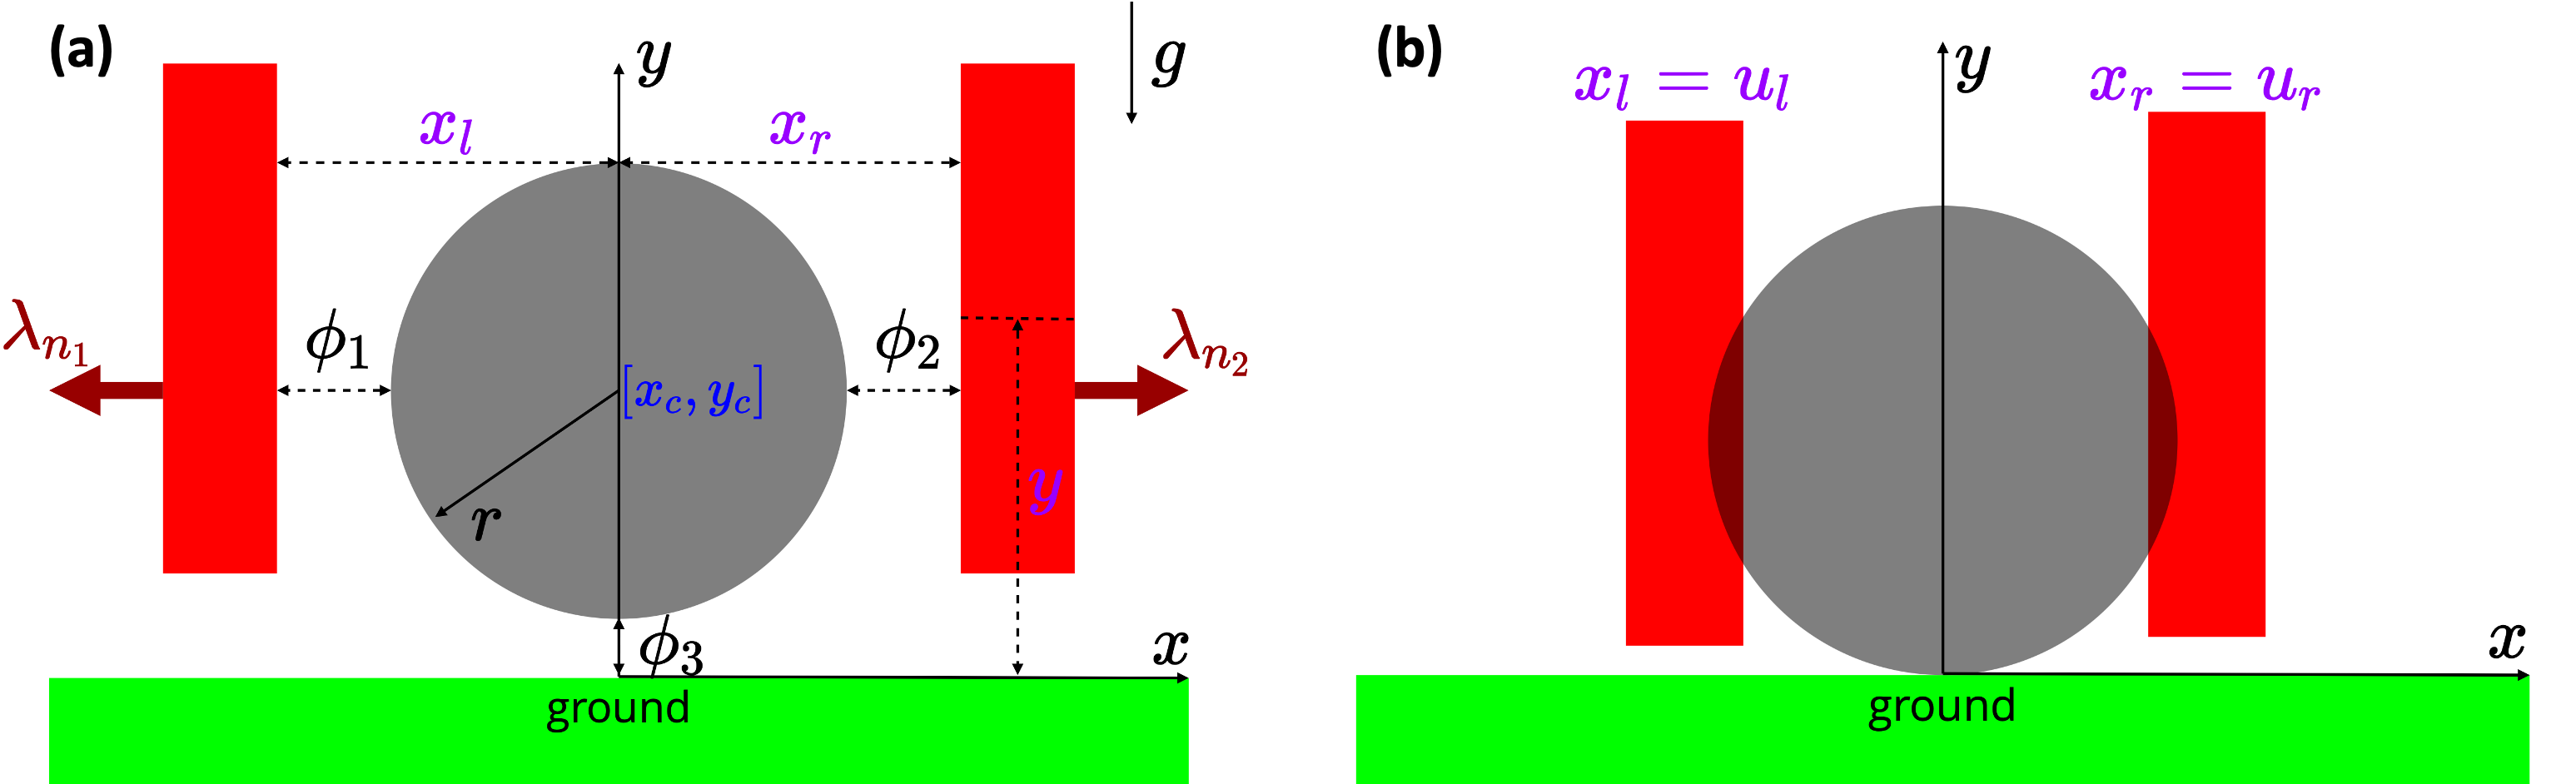
\includegraphics[width=1.0\linewidth]{figures/02_quasi_static_dynamics/gripper_ball_schematics.png}
\caption{(\textbf{a}) A planar quasi-static multibody system. The red rectangles are the actuated gripper fingers, $\qa= [x_l, x_r, y]$ and $u = [u_l, u_r, u_y]$. The gray sphere is the un-actuated manipuland, $\qu = [x_c, y_c]$. $r=0.1\mathrm{m}$. The normal contact forces associated with contact pair 1 and 2 are denoted respectively by $\lambda_{\mathrm{n}_1}$ and $\lambda_{\mathrm{n}_2}$. (\textbf{b}) A grasping command violating the non-penetration constraint.}
\label{fig:gripper_ball_schematics}
\end{figure}

As a consequence of modeling robots as prescribed motions, the robot force balance condition \eqref{eq:q_dynamics_eom:a} is replaced by 
\begin{equation}
\label{eq:naive_quasi_static_robot_motion}
\qa + \delta \qa = u.
\end{equation}

Although seemingly plausible, the simplistic robot dynamics (\ref{eq:naive_quasi_static_robot_motion}) is an ill-posed dynamical system: (\textbf{i}) it is possible to command a $u$ that violates non-penetration constraints; (\textbf{ii}) when two bodies are in contact, the contact force between them can be under-determined \cite{pang2018robust, halm2018quasi}. Instead of belonging to a niche set of contrived corner cases, such issues arise naturally and frequently in even the simplest robotic manipulation tasks. Consider the example in Fig. \ref{fig:gripper_ball_schematics}a, where the fingers are commanded to grasp the sphere. For PD-controlled grippers, it is common to command a small amount of penetration to establish contact forces. However, such commands would penetrate the object, as shown in Fig. \ref{fig:gripper_ball_schematics}b. On the other hand, even if the fingers are commanded to ``graze'' the sphere ($\phi_1 = \phi_2 = 0$), which respects non-penetration constraints, any non-negative contact force $\lambda_{\mathrm{n}_1}$ and $\lambda_{\mathrm{n}_2}$ would satisfy \eqref{eq:q_dynamics_eom:u}. This is problematic if the fingers are also commanded to move up: small contact forces would leave the sphere on the ground, but large contact forces would generate enough friction to lift up the sphere. Modeling control inputs as robot motions simply cannot determine whether the sphere moves with the hand or stays on the table.

Our impedance formulation (\ref{eq:q_dynamics_eom:a}) resolves the ill-posedness of \eqref{eq:naive_quasi_static_robot_motion} by effectively connecting $\qa$ and $u$ using springs with zero rest lengths. To illustrate how the spring helps, we focus on $x_l$, the prismatic joint of left finger in the planar grasping example in Fig. \ref{fig:gripper_ball_schematics}a. Force balance for $x_l$ is given by 
\begin{equation}
\label{eq:force_balance_xl}
    k(u_{l} - x_l) + \lambda_{\mathrm{n}_1} = 0,
\end{equation}
where $k$ is the stiffness of the spring, $k(u_{l} - x_l)$ is the spring force acting on the left finger, and $f_{n_1}$ the force from contact with the sphere.

When the left finger is not in the vicinity of the sphere (Fig. \ref{fig:actuator_with_springs}a), we have $\lambda_{\mathrm{n}_1}=0$, which together with (\ref{eq:force_balance_xl}) implies that $x_l = u_l$. Therefore, in the absence of contact, adding the spring has the same effect as (\ref{eq:naive_quasi_static_robot_motion}). On the other hand, when the left finger is commanded to squeeze the sphere (Fig. \ref{fig:actuator_with_springs}b), $x_l$ and $u_l$ are different due to the non-penetration constraint. The spring force $k(x_l - u_l)$ is balanced by the contact force $\lambda_{\mathrm{n}_1}$. 
\begin{figure}
\centering
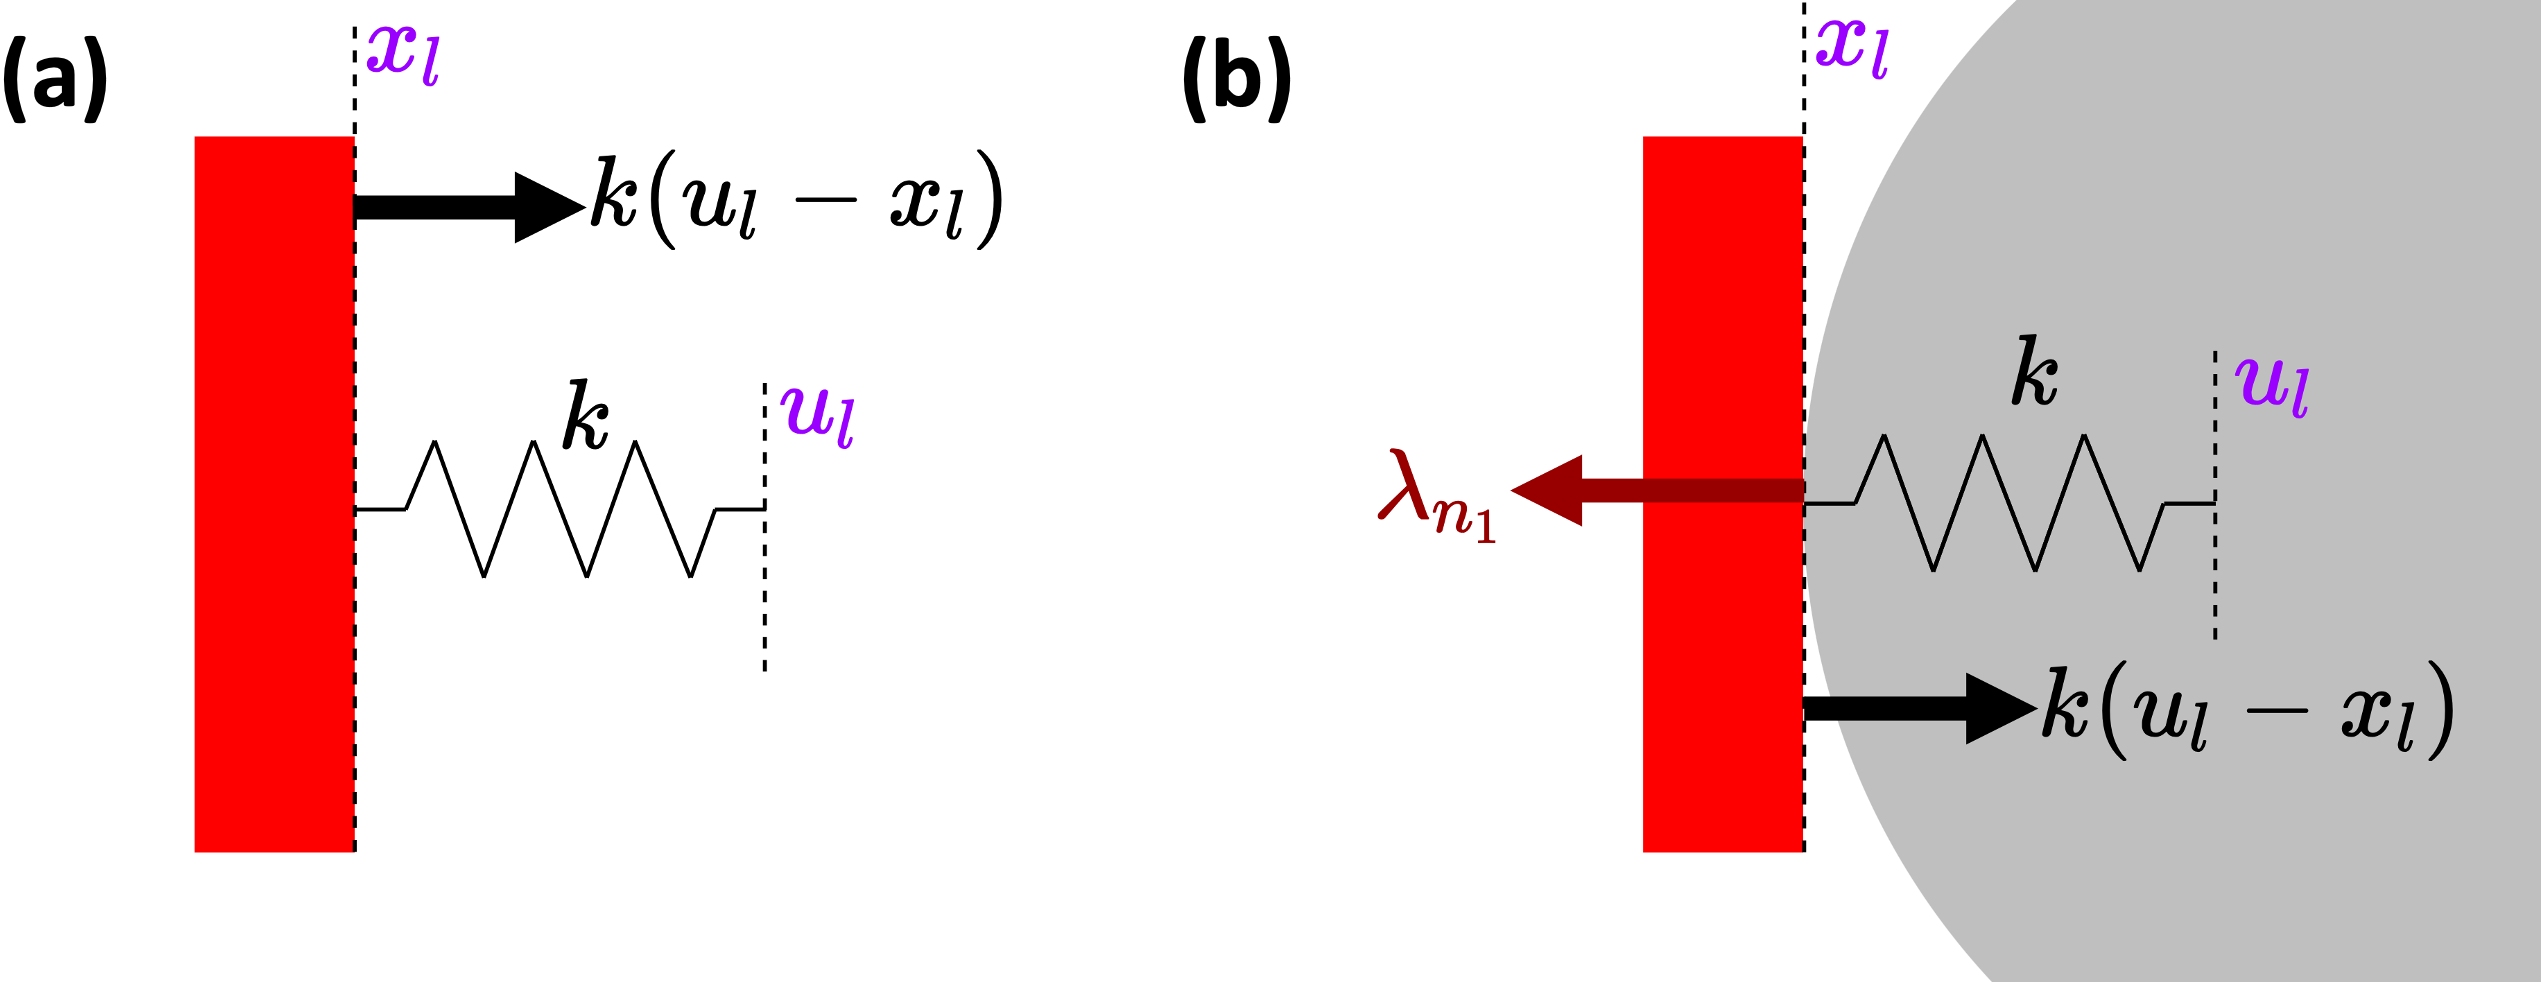
\includegraphics[width=0.90\linewidth]{figures/02_quasi_static_dynamics/actuator_with_springs.png}
\caption{Free-body diagrams of the left finger when it is (\textbf{a}) away from the sphere, and (\textbf{b}) in contact with the sphere.}
\label{fig:actuator_with_springs}
\end{figure}

The addition of the spring resolves both issues with (\ref{eq:naive_quasi_static_robot_motion}): (\textbf{i}) feasibility of the non-penetration constraint is retained by allowing $x_l$ to be different from its commanded value $u_l$; (\textbf{ii}) the magnitude of the contact force is also uniquely determined by the difference between $x_l$ and $u_l$. 

Although adding springs between $\qa$ and $u$ may seem arbitrary, it is equivalent to modeling the actuators as impedances \cite{hogan1985impedance}. For instance, the closed-loop dynamics of the KUKA iiwa arm in joint-impedance mode is:
\begin{equation}
\label{eq:controlled_iiwa_dynamics}
\mathbf{M}(q)\ddot{q} + \left(\mathbf{D}_q + \mathbf{C}(q, \dot{q}) \right) \dot{q}  + \mathbf{K}_q \left(q - u\right) = \tau_{\text{ext}},
\end{equation}
where $q$ is the joint angles of the robot arm, $\mathbf{M}(q)$ the mass matrix, $\mathbf{C}(q, \dot{q})$ the Coriolis force, $\mathbf{K}_q$ the diagonal joint stiffness matrix, $\mathbf{D}_q$ the diagonal damping matrix and $\tau_{\text{ext}}$ the joint torque generated by external contact \cite{ott2008passivity}. Discarding terms related to velocity and acceleration, the second-order dynamics (\ref{eq:controlled_iiwa_dynamics}) becomes
\begin{equation}
    \mathbf{K}_q \left(q - u\right) = \tau_{\text{ext}},
\end{equation}
which can be interpreted as the joint space version of (\ref{eq:force_balance_xl}).

\subsubsection{Bond Graph}
Bond graph is a graphical tool for describing energy flows between components of a dynamical system \cite{bondgraph}. In his seminal work on impedance control, Hogan justified modeling robots as impedances using bond graph analysis \cite{hogan1984impedance}. 

Fig. \ref{fig:bond_graph} shows bond graphs of a 1-DOF quasi-static robot pushing against a wall when the robot is modeled as prescribed motions (admittance) vs. as impedance. Both the robot and the wall are modeled as \emph{flow sources}. In Fig. \ref{fig:bond_graph}a the flows from both sources are constrained to be equal by the \emph{1 junction}, whereas in Fig. \ref{fig:bond_graph}b the flows can be different due to the spring. The flaw of modeling robots as prescribed motions is revealed clearly as a syntax error in the bond graph. In Fig. \ref{fig:bond_graph}a, the 1 junction has two \emph{strong bonds}, both of which dictate the flow. However, the syntax of 1 junction only allows one strong bond per junction.
\begin{figure}
\centering
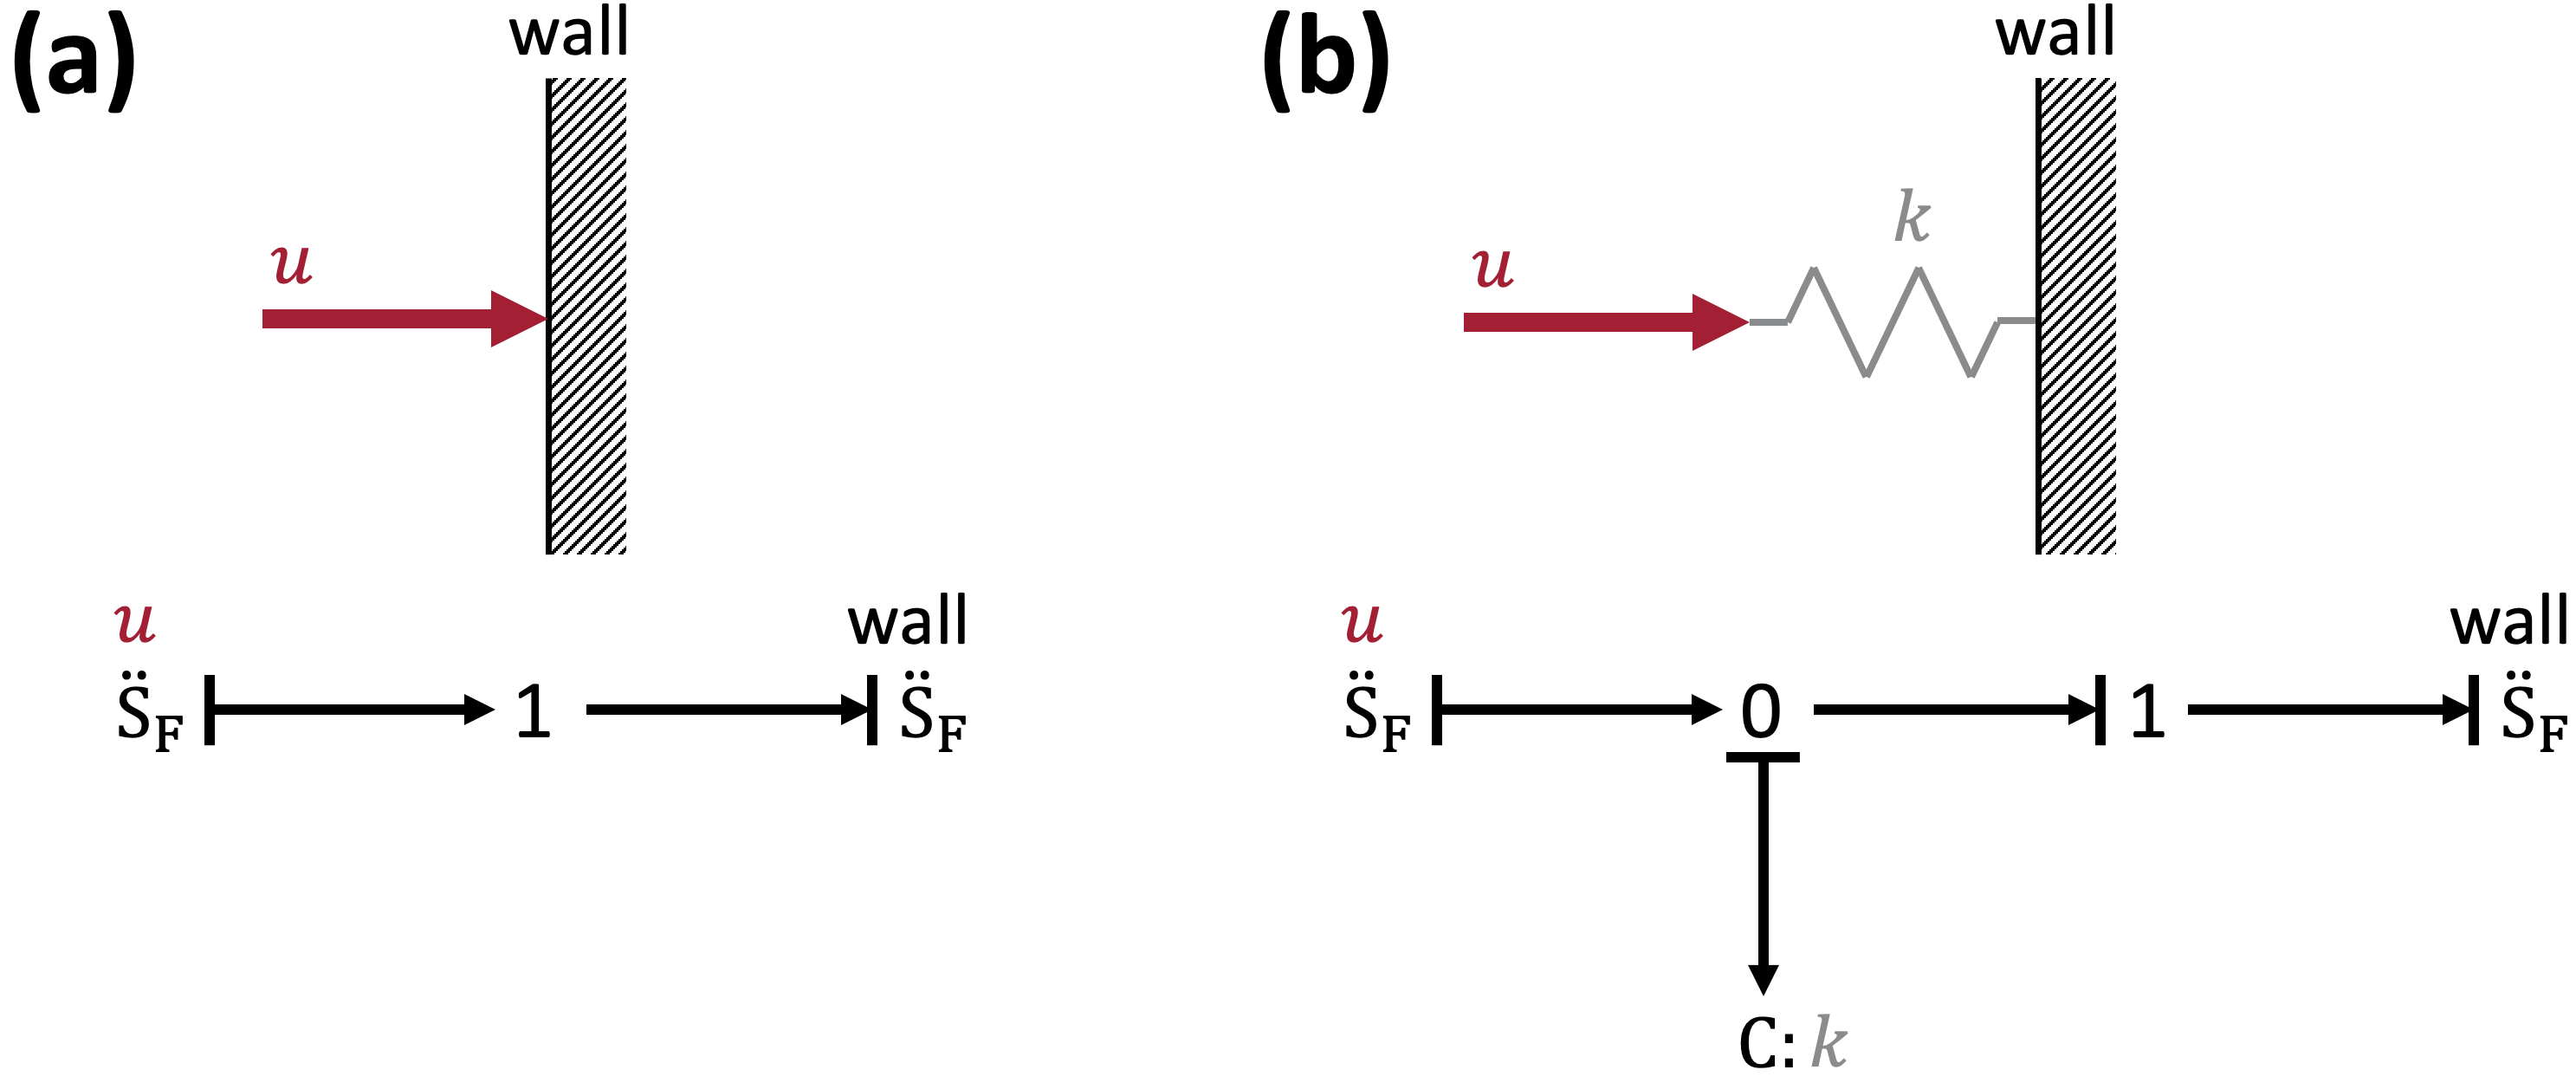
\includegraphics[width=1.0\linewidth]{figures/02_quasi_static_dynamics/bond_graph.png}
\caption{Bond graphs of a 1-DOF robot pushing against the wall. In (\textbf{a}), the robot is modeled as admittance (a prescribed motion). In (\textbf{b}), the robot is modeled as impedance. }
\label{fig:bond_graph}
\end{figure}

\subsection{Experimental Evaluation} \label{sec:quasi_static:experiments}
We want to understand the extent to which simulation accuracy is affected by the ``boundary layer'' due to Anitescu's convex relaxation of the Coulomb friction constraint, which has been illustrated in Sec. \ref{sec:quasi_static:artifacts}. By comparing the proposed CQDC dynamics and a quasi-static LCP formulation on the 2D parallel gripper system using a trajectory that involves multiple contact mode changes, we show that the difference between the two friction formulations is small for typical manipulation tasks.

We also want to ensure that quasi-static simulations stay close to their second-order counterparts for typical manipulation tasks. To this end, we compare the CQDC dynamics against a high-fidelity second-order simulator, Drake's \code{MultibodyPlant} (MBP). To make the comparison as fair as possible, we turn on the semi-analytic primal (SAP) solver \cite{castro2021unconstrained} in MBP. Similar to CQDC, SAP uses Anistecu's convex relaxation of friction constraints \cite{anitescu2006optimization}, and supports implicit integration for PD controllers\footnote{
At the time of writing this thesis, implicit PD controller is still an experimental feature of Drake, pending the merge of \url{https://github.com/RobotLocomotion/drake/pull/17674}.
Implicit integration provides stability at much larger step sizes than explicit integration. The latter has been the default integration scheme in Drake due to the separation of plant and controller into individual systems. In our earlier work \cite{pang2021convex}, we compared CQDC which uses implicit integration against Drake's MBP, which is an unfair comparison due to the difference in integration schemes. 
}.
Our comparison shows that both CQDC and SAP are stable at large integration step sizes (at least $0.5\mathrm{s}$), but CQDC seems to be better at respecting non-penetration constraints as the step size gets larger, possibly because CQDC enforces non-penetration constraints directly on positions rather than on velocities.


\subsubsection{2D Parallel Gripper}
We study the ``boundary layer'' effect of the CQDC dynamics by comparing it against an LCP-based quasi-static formulation \cite{pang2021convex} which enforces the same object and robot equations of motion in \eqref{eq:q_dynamics_eom}, but models friction using linear complementarity constraints \cite{stewart1996implicit} instead of the cone complementarity constraints \eqref{eq:friction_constraints}. 

The comparison is done on the 2D grasping example introduced in Fig. \ref{fig:gripper_ball_schematics} using a gripper trajectory that induces multiple contact mode changes between the fingers and the sphere. As the system is planar, CQDC's SOCP formulation \eqref{eq:q_dynamic_socp} reduces to the QP formulation \eqref{eq:q_dynamics_planar_qp}. We use the QP formulation for the comparison in this example. 

The simulation time step $h$ is set to $0.01\mathrm{s}$; the weight of the sphere is $10\mathrm{N}$; the stiffness for all actuated DOFs is $1000 \mathrm{N / m}$ and a friction coefficient of $0.5$ is used for all contacts. The regularization constant $\epsilon$ in \eqref{eq:q_dynamics_eom:u} is set to 0. We will use $c_{\mathrm{n}_i} \coloneqq \lambda_{\mathrm{n}_i} / h$ and $c_{\mathrm{f}_i} \coloneqq \lambda_{\mathrm{t}_i} / h$ to denote the normal and tangent components of the contact forces.

\begin{figure}
\centering
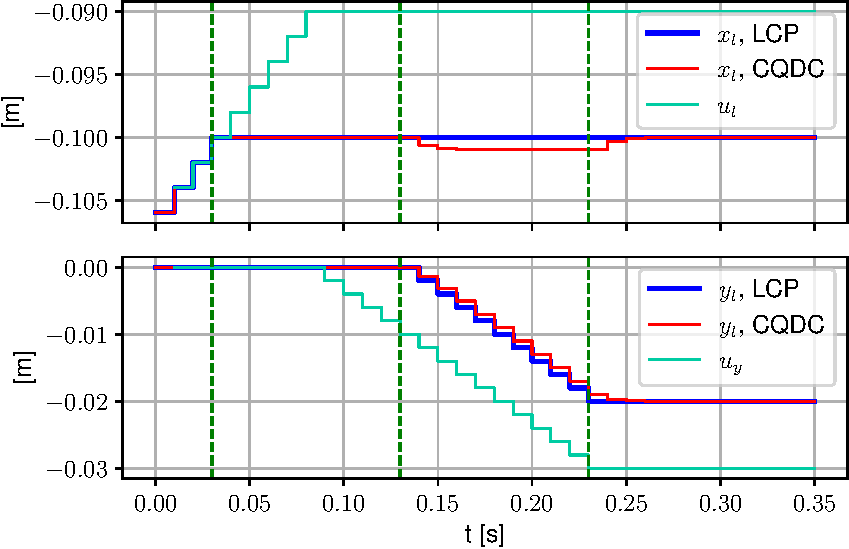
\includegraphics[width=0.75\linewidth]{figures/02_quasi_static_dynamics/xy_cmd_vs_xy_true.pdf}
\caption{Commanded and actual left finger positions for the system defined in Fig. \ref{fig:gripper_ball_schematics}, as simulated by LCP and the proposed CQDC dynamics (\ref{eq:q_dynamics_planar_qp}). 
Recall that $x_l$ and $u_l$ are respectively the commanded and actual $x$-coordinate of the left finger; $y_l$ and $u_y$ are respectively the commanded and actual $y$-coordinate of both fingers.
The right finger is not shown, as the motions and forces of the left and right fingers are symmetric about the $y$-axis. 
The green dashed vertical lines indicate contact mode changes: separation to sticking at $t=0.03\mathrm{s}$; sticking to sliding at $t=0.13\mathrm{s}$; sliding to sticking at $t=0.23\mathrm{s}$.}
\label{fig:xy_cmd_vs_xy_true}
\end{figure}

As shown in Fig. \ref{fig:xy_cmd_vs_xy_true}, the grippers start $0.006\mathrm{m}$ away from the surface of the sphere. They are first commanded to translate horizontally, touching the sphere at $t = 0.03\mathrm{s}$. The grippers continue to squeeze the object until $t = 0.08 \mathrm{s}$. Accordingly, $c_{\mathrm{n}_1}$ grows from $0\mathrm{N}$ to $10\mathrm{N}$, while $\phi_1$ stays at 0. As shown in Fig. \ref{fig:contact_force_distance}, this behavior is reproduced by both the LCP formulation and the CQDC dynamics \eqref{eq:q_dynamics_planar_qp}.

The grippers are then commanded to pull the ball downward into the ground. Although initially resisted by friction, the downward commands eventually overcome friction and slipping between the ball and the fingers starts at $t = 0.13 \mathrm{s}$. In the LCP simulation, $c_{\mathrm{n}_1}$, $c_{\mathrm{f}_1}$ and $\phi_1$ remain constant despite the contact mode transition from sticking to sliding. In the CQDC simulation, however, as sliding starts at $t = 0.13 \mathrm{s}$, a small increase in $\phi_1$ is observed, which, as explained in Section. \ref{section:anitescu_friction_sliding}, is needed by sliding under Anitescu's friction constraints. In both the LCP and CQDC simulations, $c_{\mathrm{n}_3}$ grows with the friction $c_{\mathrm{f}_1}$ in order to keep the sphere in force balance.

The downward commands stop at $t = 0.24 \mathrm{s}$, and the contact mode switches back to sticking from sliding. Once again, $c_{\mathrm{n}_1}$, $c_{\mathrm{f}_1}$ and $\phi_1$ remain constant in the LCP formulation. In contrast, the ``boundary layer'' created by sliding in the CQDC dynamics disappears as sliding stops.

\begin{figure}
\centering
\subfloat[Simulated by quasi-static LCP.]{
	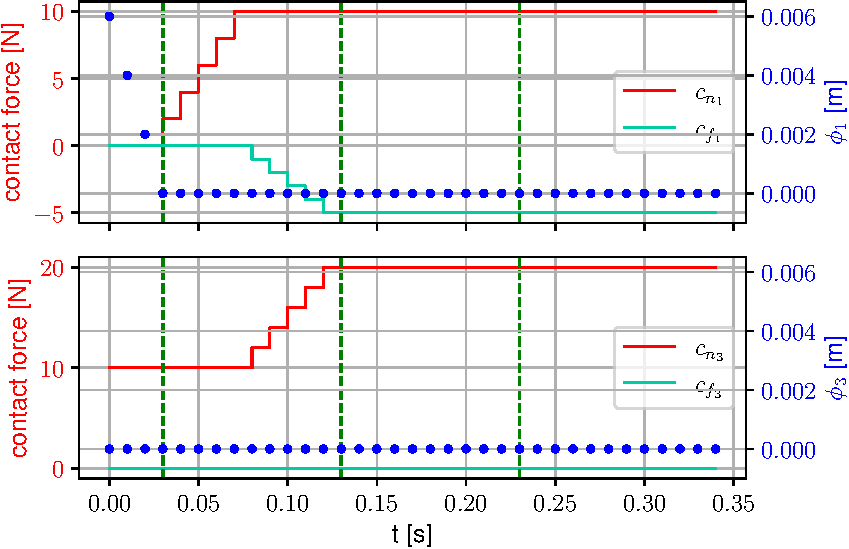
\includegraphics[width=0.75\linewidth]{figures/02_quasi_static_dynamics/contact_force_distance_lcp.pdf}
	\label{fig:contact_force_distance_lcp}
}\\
\subfloat[Simulated by the proposed CQDC dynamics (\ref{eq:q_dynamics_planar_qp}).]{
	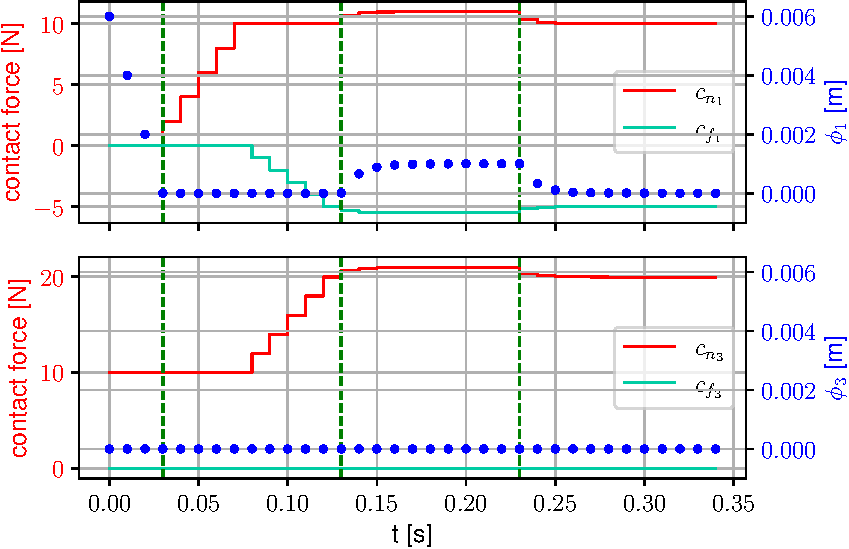
\includegraphics[width=0.75\linewidth]{figures/02_quasi_static_dynamics/contact_force_distance_qp.pdf}
	\label{fig:contact_force_distance_qp}
}
\caption{Contact force and signed distance at contact 1 and 3 of the gripper-sphere system defined in Fig. \ref{fig:gripper_ball_schematics}.}
\label{fig:contact_force_distance}
\end{figure}

\subsubsection{Iiwa Trajectory Tracking}
Our first comparison between CQDC and SAP involves tracking a reference joint-angle trajectory $q_\mathrm{ref}(\cdot)$ on a gravity-compensated and PD-controlled iiwa arm. The task only involves the smooth closed-loop dynamics of the arm \eqref{eq:controlled_iiwa_dynamics}, and does not involve any external contact. The starting and ending configurations of the reference trajectory are shown in Fig. \ref{fig:iiwa_trajectory_tracking}a and Fig. \ref{fig:iiwa_trajectory_tracking}b, respectively. We interpolate between the two configurations using a cubic spline, with maximum velocity in the middle and zero velocity at the two ends. We will denote the trajectory simulated by the CQDC dynamics as $q_\mathrm{CQDC}(\cdot)$, and SAP by $q_\mathrm{SAP}(\cdot)$.

\begin{figure}[h]
\centering
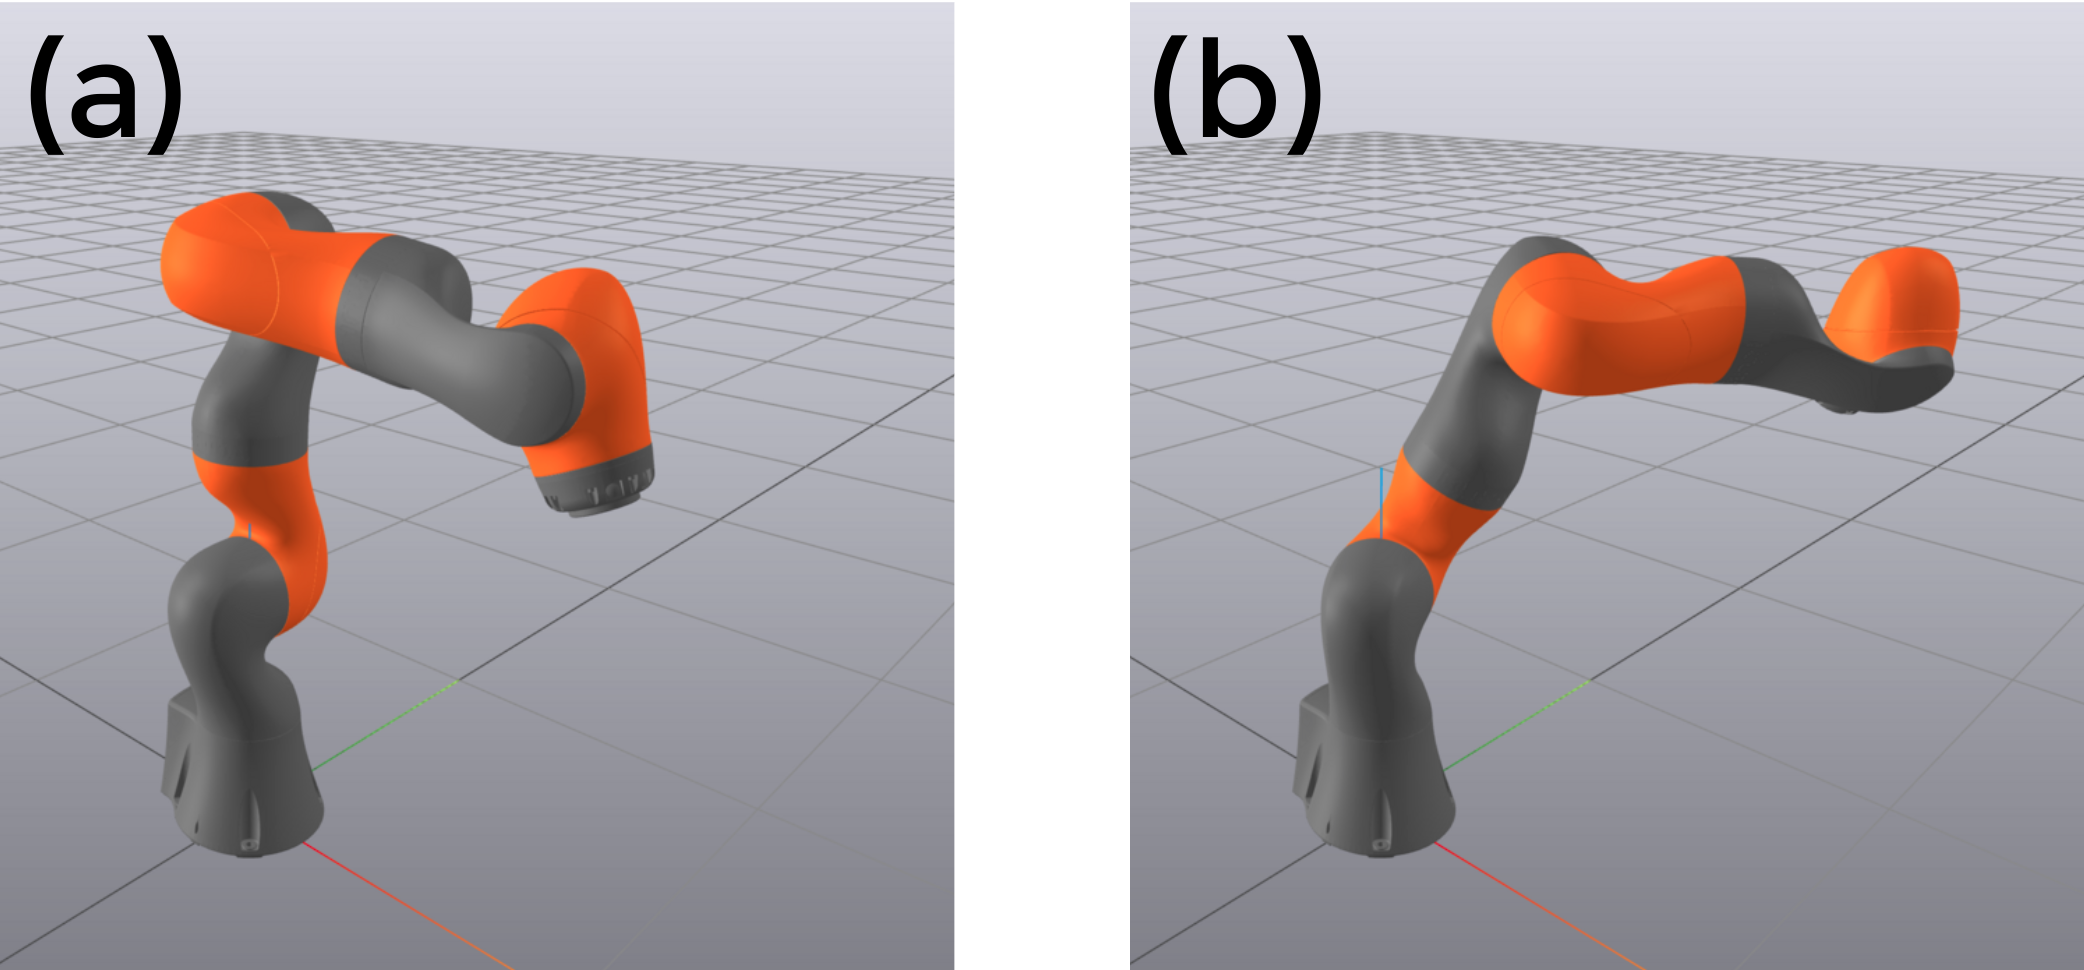
\includegraphics[width=0.70\linewidth]{figures/02_quasi_static_dynamics/iiwa_trajectory_tracking.png}
\caption{Starting (\textbf{a}) and ending (\textbf{b}) configurations of the reference joint-angle trajectory $q_\mathrm{ref}(\cdot)$.}
\label{fig:iiwa_trajectory_tracking}
\end{figure}

To evaluate the performance of the two simulators, we first define the mean error $\Delta(\cdot,\cdot)$ between two joint-angle trajectories $q_\mathrm{1}(\cdot)$ and $q_\mathrm{2}(\cdot)$ as
\begin{equation}
\label{eq:mean_trajectory_error}
\Delta(q_\mathrm{1}, q_\mathrm{2}) \coloneqq 
\frac{1}{T}
\int^T_{0} d(q_\mathrm{1}(t), q_\mathrm{2}(t))\mathrm{d}t,
\end{equation}
where $T$ denotes the duration of the trajectories; $d(\cdot, \cdot)$ is the distance metric for the space of joint angles, which is simply the Euclidean 2-norm.

For different simulation step sizes $h$, the mean errors between simulated and reference trajectories, i.e. $\Delta(q_\mathrm{CQDC/SAP}, q_\mathrm{ref})$, are shown in Fig. \ref{fig:iiwa_trajectory_tracking_error_vs_time_step}. The error increases with $h$, but remains small even for very large $h$ ($h=0.5\mathrm{s}$). In addition, as CQDC has no inertia, it tends to be slightly better at tracking the reference, especially as $h$ gets smaller.

\begin{figure}[h]
\centering
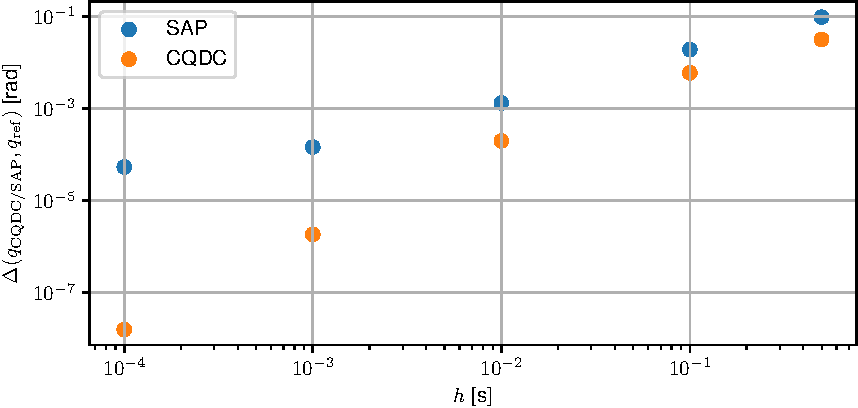
\includegraphics[width=0.8\linewidth]{figures/02_quasi_static_dynamics/iiwa_trajectory_tracking_error_vs_time_step.pdf}
\caption{Mean tracking error $\Delta(q_\mathrm{CQDC/SAP}, q_\mathrm{ref})$ for trajectories simulated using the CQDC dynamics or SAP at different simulation step sizes $h$.}
\label{fig:iiwa_trajectory_tracking_error_vs_time_step}
\end{figure}


\subsubsection{Box Stacking with Iiwa}
Our second comparison between CQDC and SAP focuses on a complex 3D system with many contacts, as shown in Fig. \ref{fig:iiwa_cube_stacking}. The system has 10 cubes and 69 DOFs. The task is the robot picking up the red-and-grey cube and placing it on the stack. There is on average 56 contacts per time step during the execution of the task.
\begin{figure}
\centering
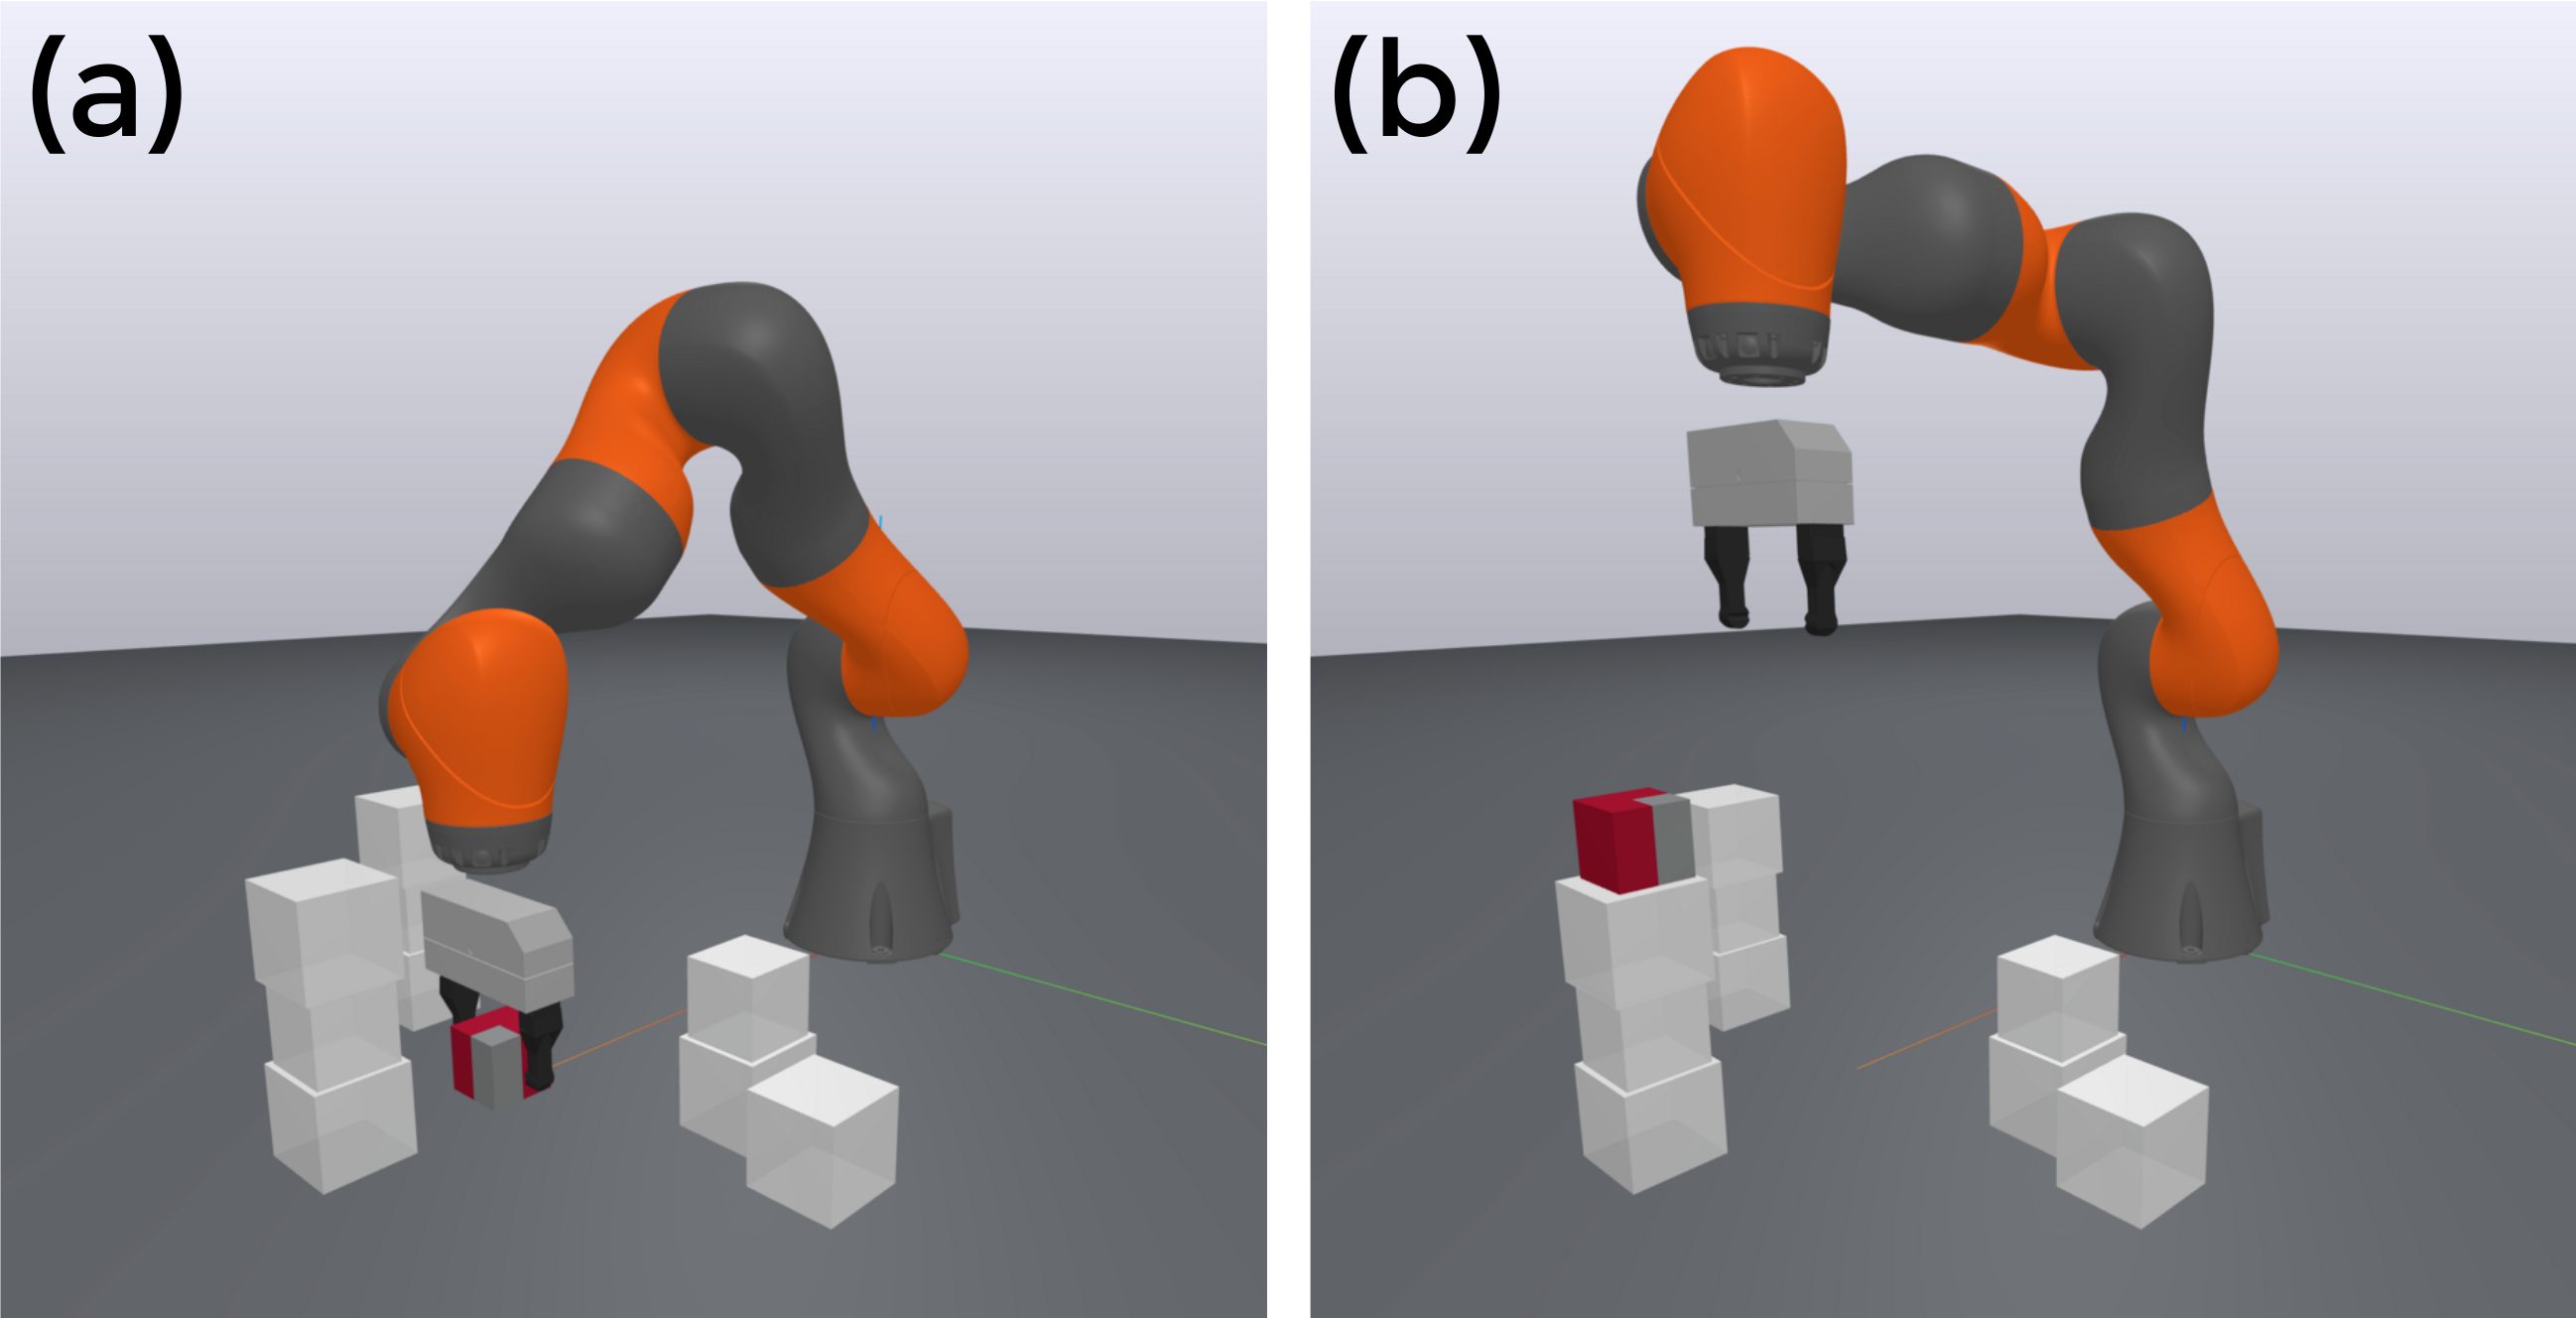
\includegraphics[width=0.75\linewidth]{figures/02_quasi_static_dynamics/start_and_final_configurations.png}
\caption{KUKA IIWA robot stacking cubes. The red-and-grey cube has a quadrant colored grey to indicate its orientation. The red-and-grey cube starts off on the ground (\textbf{a}) and is placed on a stack of cubes and rotated by 90 degrees (\textbf{b}).}
\label{fig:iiwa_cube_stacking}
\end{figure}

Firstly, although both CQDC and SAP are stable for large step sizes (at least $h=0.5\mathrm{s}$), CQDC is accurate for all step sizes, whereas the accuracy of SAP starts to degrade significantly as $h$ crosses a threshold. 
Similar to the iiwa trajectory tracking example, we compare trajectories of the red-and-grey cube using the mean error defined by \eqref{eq:mean_trajectory_error}. Instead of comparing against a reference trajectory, we define the \emph{ground truth} trajectory of the box, $q_\mathrm{GT}^\mathrm{u}(\cdot)$, as the trajectory generated by SAP using $h=5 \times 10^{-5} \mathrm{s}$.
As shown in Fig. \ref{fig:error_vs_time_step}, the mean error of the box pose between CQDC and the ground truth, $\Delta (q_\mathrm{CQDC}^\mathrm{u}, q_\mathrm{GT}^\mathrm{u})$, remains small up to $h=0.1\mathrm{s}$ and is still moderate at $h=0.5\mathrm{s}$, indicating that a large $h$ can be used for planning without impacting accuracy.
In contrast, $\Delta (q_\mathrm{SAP}^\mathrm{u}, q_\mathrm{GT}^\mathrm{u})$ becomes large for $h \geq 0.01 \mathrm{s}$.
\begin{figure}
\centering
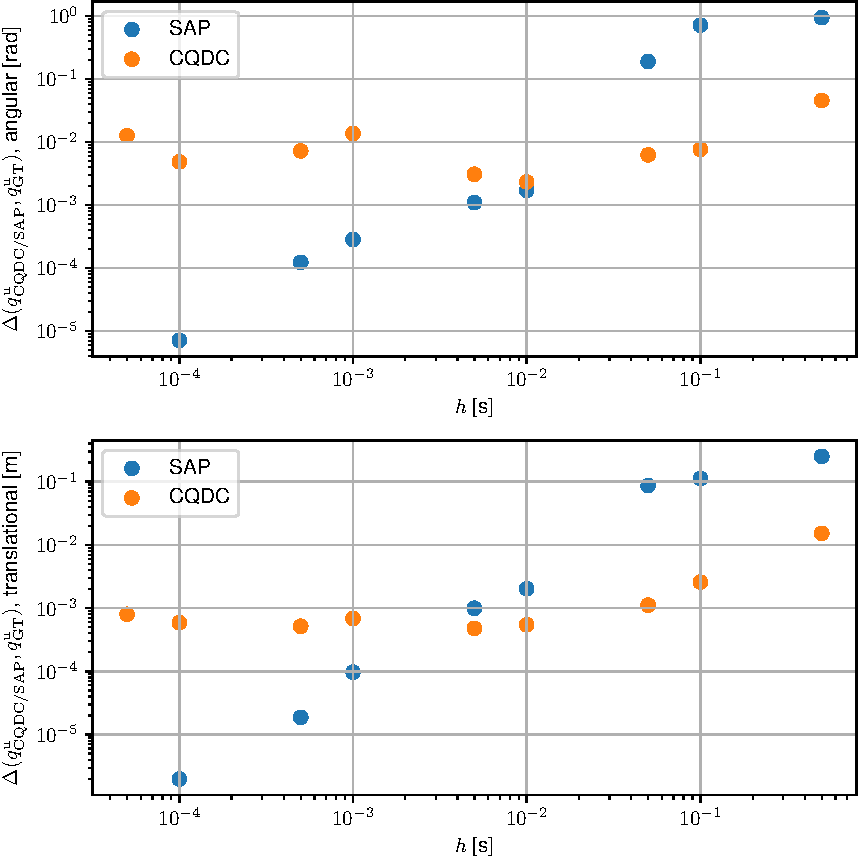
\includegraphics[width=0.8\linewidth]{figures/02_quasi_static_dynamics/error_vs_time_step.pdf}
\caption{Angular and translational mean error of the pose of the red-and-grey box, $\Delta (q_\mathrm{CQDC/SAP}^\mathrm{u}, q_\mathrm{GT}^\mathrm{u})$, at different step sizes $h$.
As shown in Fig. \ref{fig:iiwa_cube_stacking}, the box is picked up, rotated, and placed on the stack of cubes.
The ground truth trajectory, $q_\mathrm{GT}^\mathrm{u}$, is defined as the trajectory generated by SAP with $h=5\times10^{-5}\mathrm{s}$.
In the computation of the mean error $\Delta(\cdot, \cdot)$, the distance function $d(\cdot, \cdot)$ is the Euclidean 2-norm for translation, and the absolute difference in angle for rotation.
}
\label{fig:error_vs_time_step}
\end{figure}

The reason behind the larger error of SAP at larger step sizes is shown in Fig. \ref{fig:iiwa_cube_stacking_sap_vs_cqdc}. With SAP, it appears that contacts become softer as $h$ increases, eventually leading to boxes sinking into each other and the ground. 
\begin{figure}
\centering
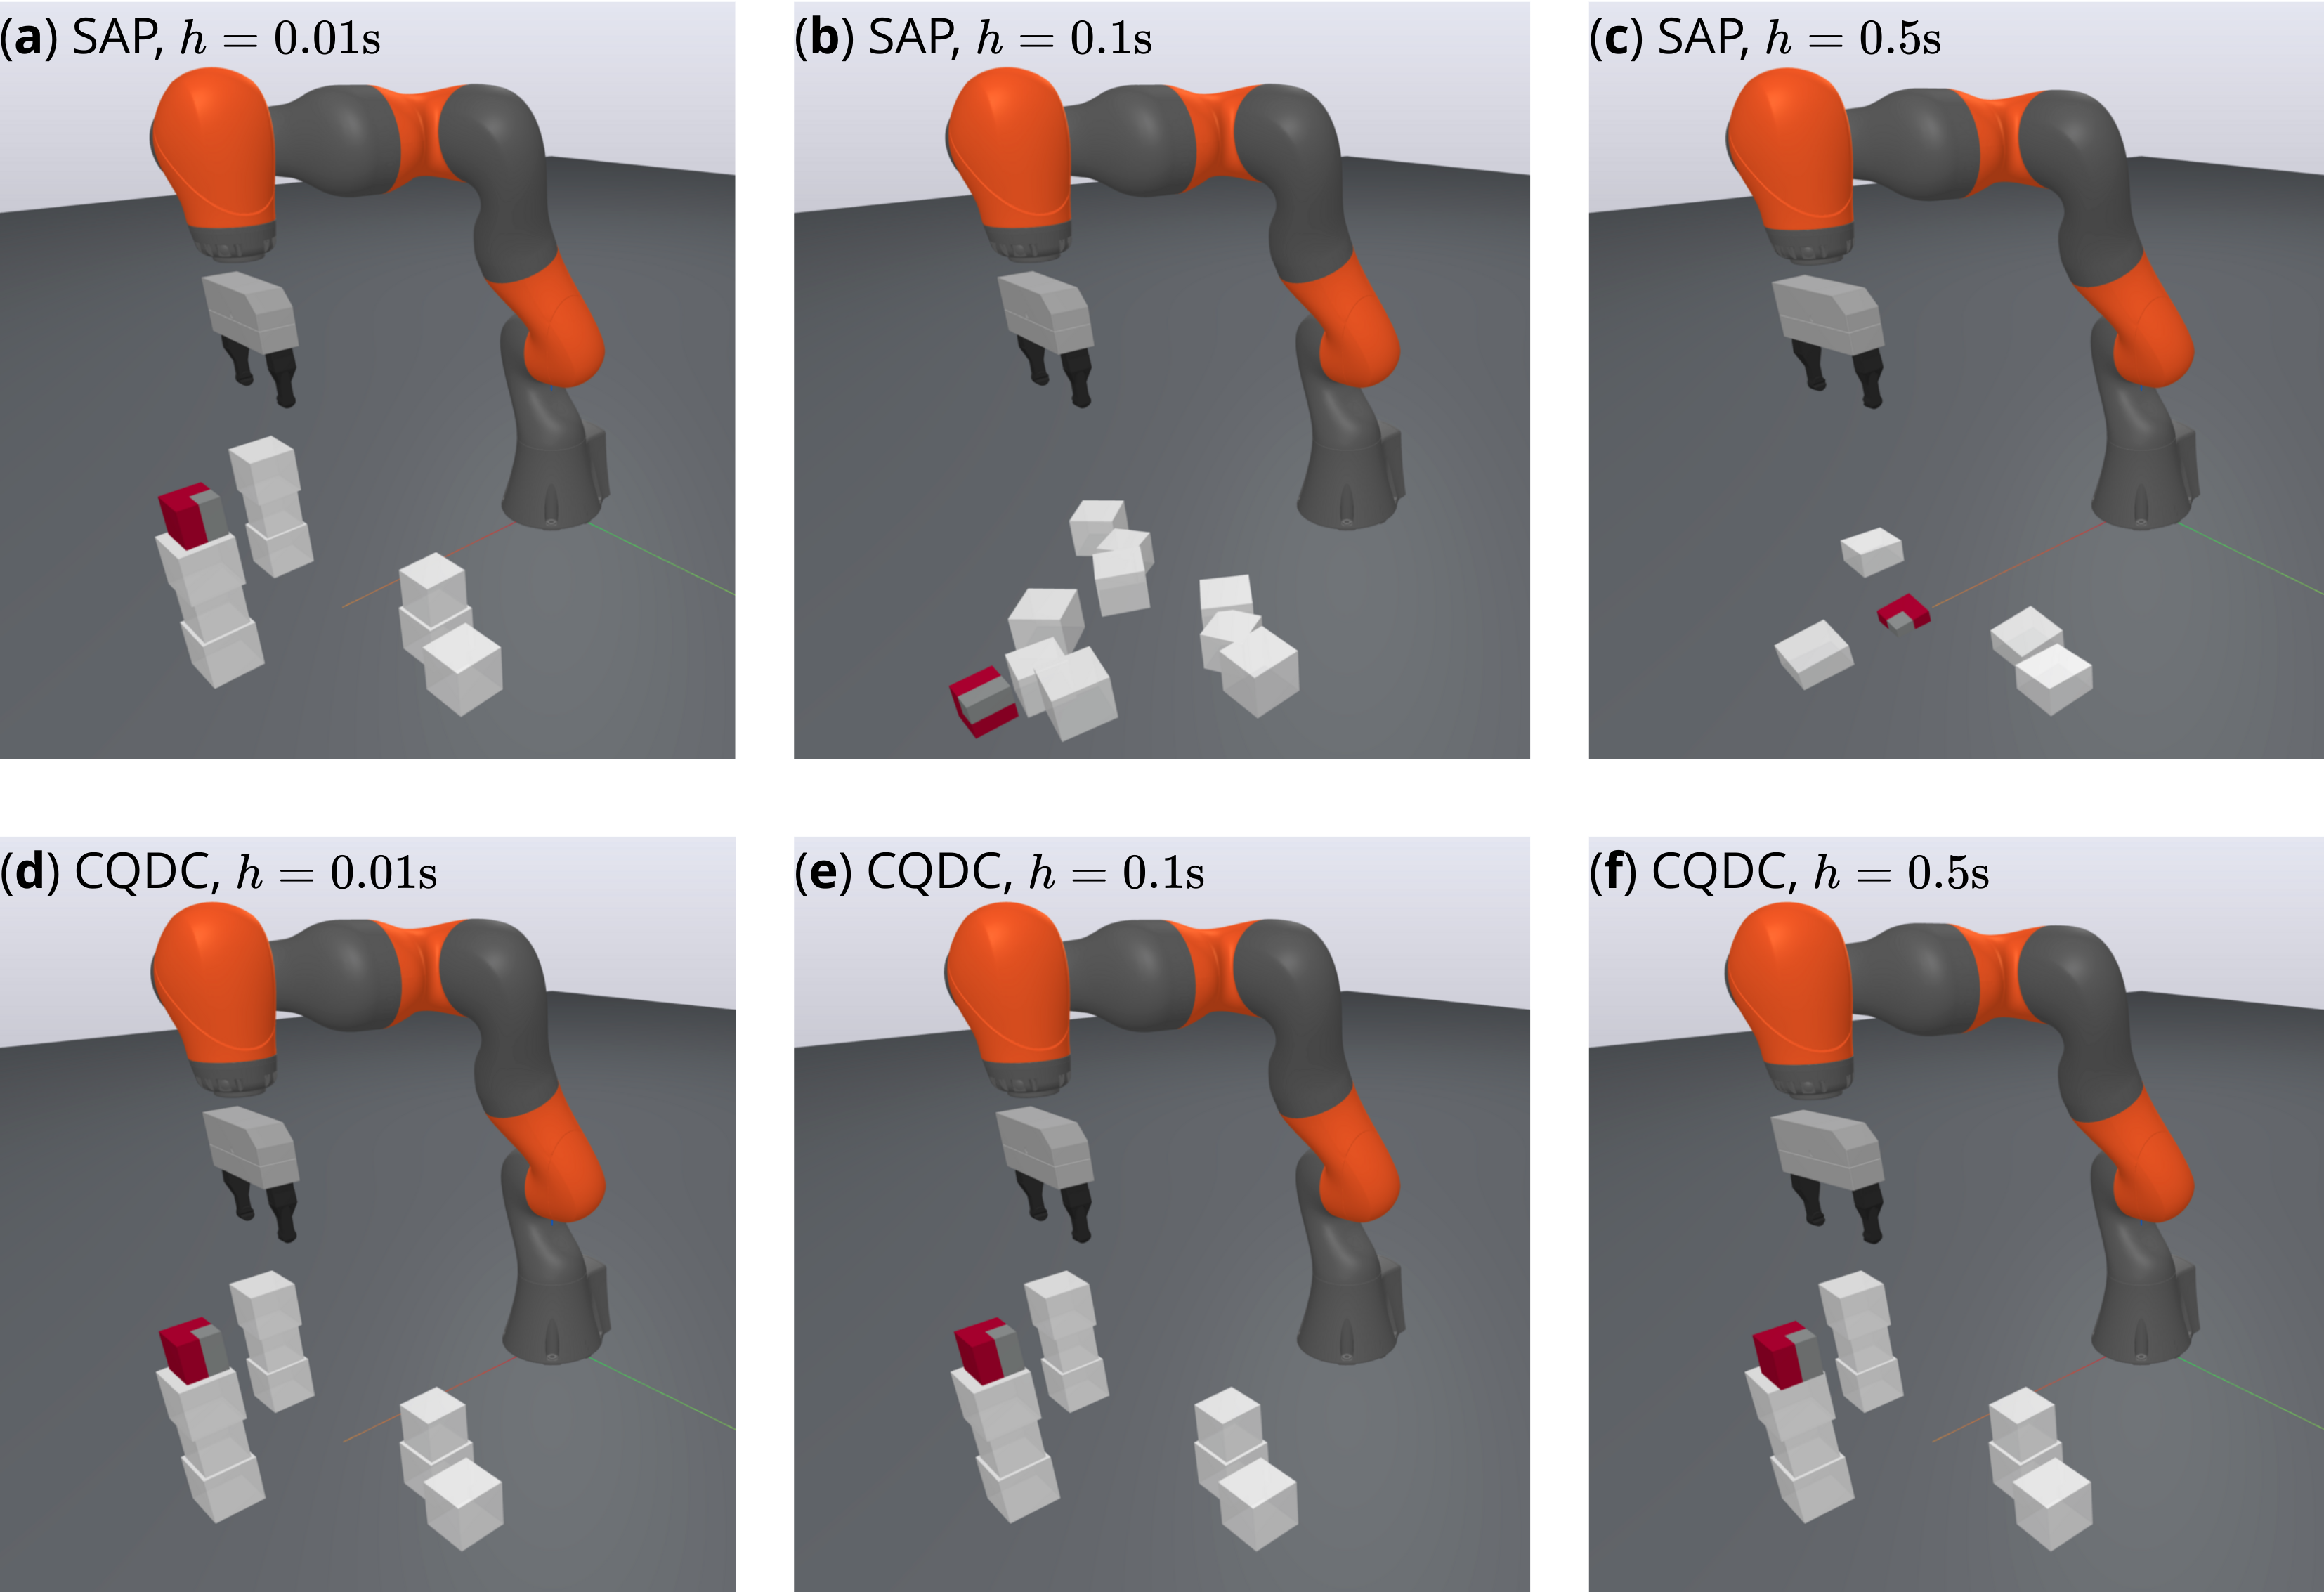
\includegraphics[width=1.0\linewidth]{figures/02_quasi_static_dynamics/sap_vs_cqdc.png}
\caption{Final configurations of the box stacking task shown in Fig. \ref{fig:iiwa_cube_stacking}, simulated using SAP (\textbf{a}-\textbf{c}) and CQDC (\textbf{d}-\textbf{f}).}
\label{fig:iiwa_cube_stacking_sap_vs_cqdc}
\vspace{-0.5cm}
\end{figure}

Good simulation accuracy by the CQDC dynamics at large $h$ is also evident in the pose trajectory of the box, which is shown in Fig. \ref{fig:cube_pose}. The translational trajectories are almost identical to the ground truth for all $h$ except $h=0.5\mathrm{s}$, but even at $h=0.5\mathrm{s}$ the error is just slightly more than 1cm. There is also no significant deviation of the object orientation from the ground truth. 
\begin{figure}
\centering
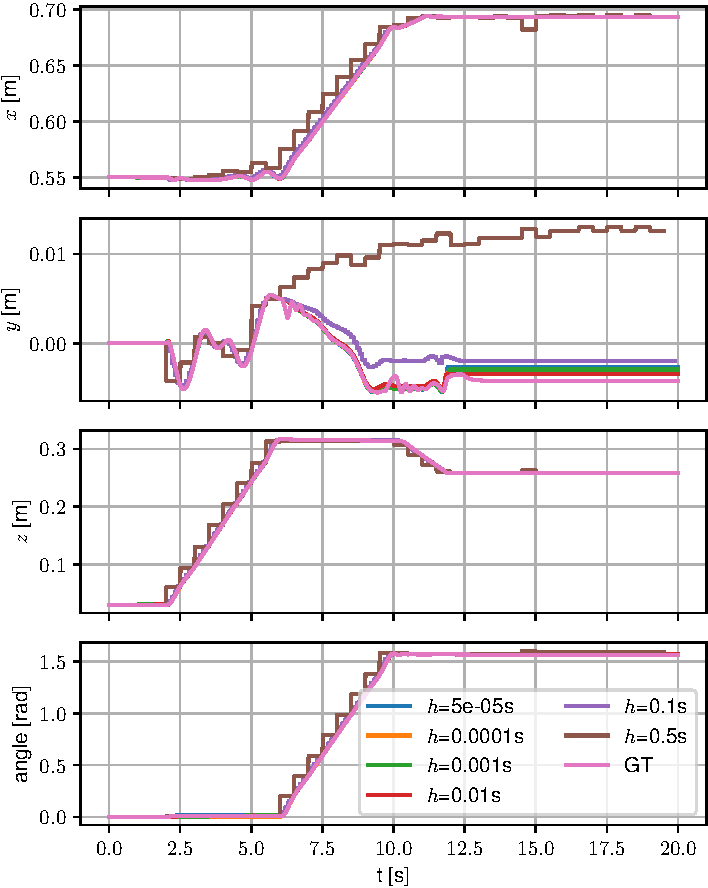
\includegraphics[width=0.9\linewidth]{figures/02_quasi_static_dynamics/box0_pose.pdf}
\caption{Trajectories of the red cube in Fig. \ref{fig:iiwa_cube_stacking}, including the ground truth (GT) and the ones generated using the CQDC dynamics with different step sizes $h$. $x$, $y$ and $z$ are the cube's center of mass coordinates in world frame. Angle comes from the axis-angle representation of the cube's orientation relative to world frame. Here the angle plot represents a rotation about the world $y$-axis by 90 degrees. The larger $y$ error at $h=0.5\mathrm{s}$ is caused by the gripper clipping the corner of the red-and-grey box when the gripper retreats from the box after placing it on the top of the stack. Due to the large $h$, the gripper's motion is interpolated between an upward segment and a horizontal segment. This error is visible by the difference of a few pixels between Fig. \ref{fig:iiwa_cube_stacking_sap_vs_cqdc}e
and Fig. \ref{fig:iiwa_cube_stacking_sap_vs_cqdc}f.
}
\label{fig:cube_pose}
\end{figure}

Lastly, the CQDC dynamics (\ref{eq:q_dynamic_socp}) scales well with the number of DOFs and contacts. The mean time of solving SOCP (\ref{eq:q_dynamic_socp}) using Gurobi \cite{gurobi} for the box stacking task in Fig. \ref{fig:iiwa_cube_stacking} is less than 10ms on a Mac mini with Intel i7-8700B CPU and 64GB of RAM. 

\newpage
\section{Smoothing of Contact Dynamics} \label{sec:smoothing}
This section discusses how the proposed CQDC dynamics (Sec. \ref{sec:q_dynamics:cqdc}) can be smoothed, so that we can efficiently make good local linear approximations that are useful for planning.
We will begin with a summary of the randomized and analytic smoothing schemes proposed in \cite[Section II]{pang2022global} (Sec. \ref{sec:smoothdynamics}). 
We will then discuss how the proposed quasi-static dynamics model readily supports both randomized (Sec. \ref{sec:randomizedmoothing}) and analytic smoothing (Sec. \ref{sec:analyticsmoothing}), and how the two schemes are related (Sec. \ref{sec:smoothing_equivalence}). 


\subsection{Smoothing Schemes for Dynamical Systems}
\label{sec:smoothdynamics}
This subsection summarizes three different smoothing schemes for dynamical systems of the form $x_+ = f(x, u)$ \eqref{eq:f_x_u}. The smoothing schemes are (\textbf{i}) analytic smoothing, (\textbf{ii}) first-order randomized smoothing and (\textbf{iii}) zeroth-order randomized smoothing.

Although the three schemes all compute the same quantity, they require different levels of access of the dynamics $f(\cdot, \cdot)$. Analytic smoothing utilizes the structure of $f(\cdot, \cdot)$ to efficiently compute a smoothed version of it, and therefore requires white-box access to $f(\cdot, \cdot)$. In contrast, randomized smoothing schemes achieve smoothing via sampling: first-order randomized smoothing needs black-box access to $f(\cdot, \cdot)$, $\DfDx{f}{x}(\cdot, \cdot)$ and $\DfDx{f}{u}(\cdot, \cdot)$, whereas zeroth-order randomized smoothing only needs black-box access to $f(\cdot, \cdot)$.

We use $(\mathbf{A}(\bar{x},\bar{u}),\mathbf{B}(\bar{x},\bar{u}),c(\bar{x},\bar{u}))$ to parameterize the linear system $\bar{f}$ that best describes $f$ around some nominal point $(\bar{x},\bar{u})$, 
\begin{equation}
    \begin{aligned}
    \bar{f}(x,u) = \mathbf{A}(\bar{x},\bar{u})\underbrace{(x-\bar{x})}_{=:\delta x } + \mathbf{B}(\bar{x},\bar{u})\underbrace{(u-\bar{u})}_{=:\delta u} + c(\bar{x},\bar{u}).
    \end{aligned}
\end{equation}
For dynamical systems, the Taylor expansion requires the system Jacobian, 
\begin{equation}\label{eq:linearization}
    \begin{aligned}
    \mathbf{A}(\bar{x},\bar{u}) & = \frac{\partial}{\partial x}f(x,u)|_{x=\bar{x},u=\bar{u}} \\
    \mathbf{B}(\bar{x},\bar{u}) & =\frac{\partial}{\partial u}f(x,u)|_{x=\bar{x},u=\bar{u}} \\
    c(\bar{x},\bar{u}) & = f(\bar{x},\bar{u}).
    \end{aligned}
\end{equation}
The \emph{smooth surrogate} of $f(x,u)$ can be defined as
\begin{equation}
\label{eq:smooth_surrogate_definition}
    f_\rho(x,u) \coloneqq \mathbb{E}_{w\sim\rho}[f(x+w^x,u+w^u)],
\end{equation}
where $\rho$ is a probability distribution, $w^x$ is the component of $w$ that corresponds to $x$, and $w^u$ is defined similarly. The model parameters of the locally linear model $\bar{f}_\rho$ are given as follows:
\begin{equation}
\label{eq:ABc_rho}
    \begin{aligned}
    \mathbf{A}_\rho(\bar{x},\bar{u}) & =  \frac{\partial}{\partial x}\mathbb{E}_{w\sim\rho}[f(x+w^x,u+w^u)]|_{x=\bar{x},u=\bar{u}} \\
    \mathbf{B}_\rho(\bar{x},\bar{u}) & =  \frac{\partial}{\partial u}\mathbb{E}_{w\sim\rho}[f(x+w^x,u+w^u)]|_{x=\bar{x},u=\bar{u}} \\
    c_\rho(\bar{x},\bar{u}) & = \mathbb{E}_{w\sim\rho}[f(\bar{x}+w^x,\bar{u}+w^u)].
    \end{aligned}
\end{equation}
In the remaining sections, we shorthand the notation and refer to the model parameters as a matrix instead of a function for compactness (e.g. $\mathbf{A}_\rho$ instead of $\mathbf{A}_\rho(\bar{x},\bar{u})$). 

\subsubsection{Analytic Smoothing}
Analytic smoothing is done by explicit computation of $f_\rho$ as defined in \eqref{eq:smooth_surrogate_definition}. In general, it is difficult to compute $f_\rho$ for arbitrary functions $f$ and smoothing kernels $\rho$. In Sec. \ref{sec:analyticsmoothing}, we introduce a method for computing $f_\rho$ when $f$ is the CQDC dynamics.

\subsubsection{First-Order Randomized Smoothing}
We use the following estimators for first-order randomized smoothing of dynamical systems,
\begin{subequations}
\label{eq:montecarlo_ABc}
\begin{align}
\mathbf{A}_\rho & \approx \textstyle \frac{1}{N}\sum^N_{i=1} \left[\textstyle\frac{\partial}{\partial x}f(\bar{x}+w_i^x,\bar{u}+w_i^u\right] \quad w_i\sim \rho \label{eq:montecarlo_ABc:A} \\ 
\mathbf{B}_\rho & \approx \textstyle \frac{1}{N}\sum^N_{i=1} \left[\textstyle\frac{\partial}{\partial u}f(\bar{x}+w_i^x,\bar{u}+w_i^u)]\right] \quad w_i\sim \rho \\ 
c_\rho & \approx \textstyle \frac{1}{N}\sum^N_{i=1} \left[\textstyle f(\bar{x}+w_i^x,\bar{u}+w_i^u)]\right] \quad w_i\sim \rho \label{eq:montecarlo_ABc:c} 
\end{align}
\end{subequations}
where $\partial f/\partial x$, and $\partial f/\partial u$ are Jacobians of the dynamics.

\subsubsection{Zeroth-Order Randomized Smoothing}
We estimate the gradients using least-squares when $\rho$ is Gaussian:
\begin{equation}
\label{eq:montecarlo_ABc_zero}
\mathbf{A}_\rho,\mathbf{B}_\rho  = \underset{\mathbf{A,B}} {\text{argmin}}\textstyle\sum^N_{i=1}
 \| f(\bar{x}+w_i^x,\bar{u}+w_i^u) - \mathbf{A} w_i^x - \mathbf{B} w_i^u - c_\rho\|^2_2
\end{equation}
where $c_\rho$ is computed with \eqref{eq:montecarlo_ABc:c}.


\subsection{Randomized Smoothing of Contact Dynamics} \label{sec:randomizedmoothing}
We follow the method in Sec. \ref{sec:smoothdynamics} in order to perform randomized smoothing of the contact dynamics. For first-order randomized smoothing, we utilize \eqref{eq:montecarlo_ABc} with access to gradients of the contact dynamics obtained in Sec.\ref{sec:quasi_dynamic_derivatives}. We similarly do zero-order randomized smoothing using \eqref{eq:montecarlo_ABc_zero}. As the state consists of only the system configuration $q$ for quasi-static systems, we assume we compute a local model around some nominal state-input pair $(\bar{q},\bar{u})$ from here onward.

However, there is a caveat in the randomized smoothing scheme: if the sampling distribution $\rho$ has infinite support, the sampled state $\bar{q} + w^q_i$ could violate the non-penetration constraint for rigid-bodies, i.e. $\phi(\bar{q} + w^q_i) < 0$ for some $i$.

Although reasoning about the dynamics $f(q, u)$ with an infeasible (penetrating) $q$ may seem ill-posed \cite{contactkalmanfilter}, we can \emph{define} the dynamics from an infeasible $q$ as the projection of $q$ to the ``nearest'' point in the feasible (non-penetrating) set. The notion of nearest can be defined in terms of the work required to move the system configuration by $\dq$, which is precisely the quadratic cost \eqref{eq:q_dynamic_socp:cost} (divided by the step size $h$). This projection problem can then be written as
\begin{subequations}
\label{eq:projection_as_optimization}
\begin{align}
\underset{\dq}{\minimize} \; &\frac{1}{2} \dq^\intercal \mathbf{Q} \dq + b^\intercal \dq, \; \text{subject to} \\
& \phi_i(q + \delta q) \geq 0, \; i \in \{1 \dots \nC\}, \label{eq:projection_as_optimization:constraint}
\end{align}
\end{subequations}
where \eqref{eq:projection_as_optimization:constraint} is the non-linear non-penetration constraint. 

While the projection in \eqref{eq:projection_as_optimization} is difficult to solve in general, we can linearize the constraint \eqref{eq:projection_as_optimization:constraint} in order to locally approximate the problem as a QP. When the constraint is linearized, the problem remarkably becomes equivalent to the frictionless special case of the CQDC dynamics \eqref{eq:q_dynamic_socp}. In other words, projection is simply another interpretation of what the CQDC dynamics does within the penetrating regime, and no other explicit treatment is required for projection other than the evaluation of CQDC dynamics. In practice, due to the local nature of linearization, we use a low-variance distribution $\rho$ to sample states, though higher variance can be used for inputs.

When samples within the penetrating regime are projected onto the boundary of the feasible set and then averaged, the expected value of such a distribution creates a \emph{stochastic force field} that pushes the object away from feasible set's boundary. We illustrate this phenomenon through a simple example. 

\begin{example}\label{ex:projection}\normalfont\textbf{(The Stochastic Force Field)} Consider the dynamics of an unactuated 1D block with a wall occupying $q \leq 0$ (Fig. \ref{fig:projection}a), such that the physical dynamics is identity \emph{if} the block is in a non-penetrating configuration, $f(q)=q$ if $q\geq 0$. The dynamics within the penetrating regime is not well-defined physically; yet, applying the quasi-dynamic equations of motions \eqref{eq:projection_as_optimization} to this system gives 
\begin{subequations}
\label{eq:projection}
\begin{align}
\underset{\delta q}{\minimize} \; &\frac{1}{2} m (\delta q)^2, \; \text{subject to} \\
& q + \delta q \geq 0.
\end{align}
\end{subequations}
which has the following solution,
\begin{equation}
\label{eq:1d_projection_solution}
f(q) = q + \delta q =  \begin{cases}
    q & \text{ if } q \geq 0  \text{ (no penetration) }\\
    0 & \text{ else } \text{ (penetration) }\\
\end{cases}
\end{equation}

One interpretation of \eqref{eq:1d_projection_solution} is that configurations inside the wall gets projected onto the wall. By taking an average according to such dynamics, the expectation pushes the box away from the wall as illustrated in Fig. \ref{fig:projection}, which creates a \emph{stochastic force field}. Note that with this interpretation, the gradients are also well-defined within the penetrating regime - an infinitesimal change of position in the penetrating configuration does not have any effect on the location of projection in this example, thus $\partial f(q)/\partial q=0$ if $q < 0$. For more complex geometries, the location of projection changes due to changes in the surface, which we connect back to the presence of the $\partial \mathbf{J}/\partial q$ and $\partial \phi/\partial q$ terms in \eqref{eq:DdqDq}.

\begin{figure}
\centering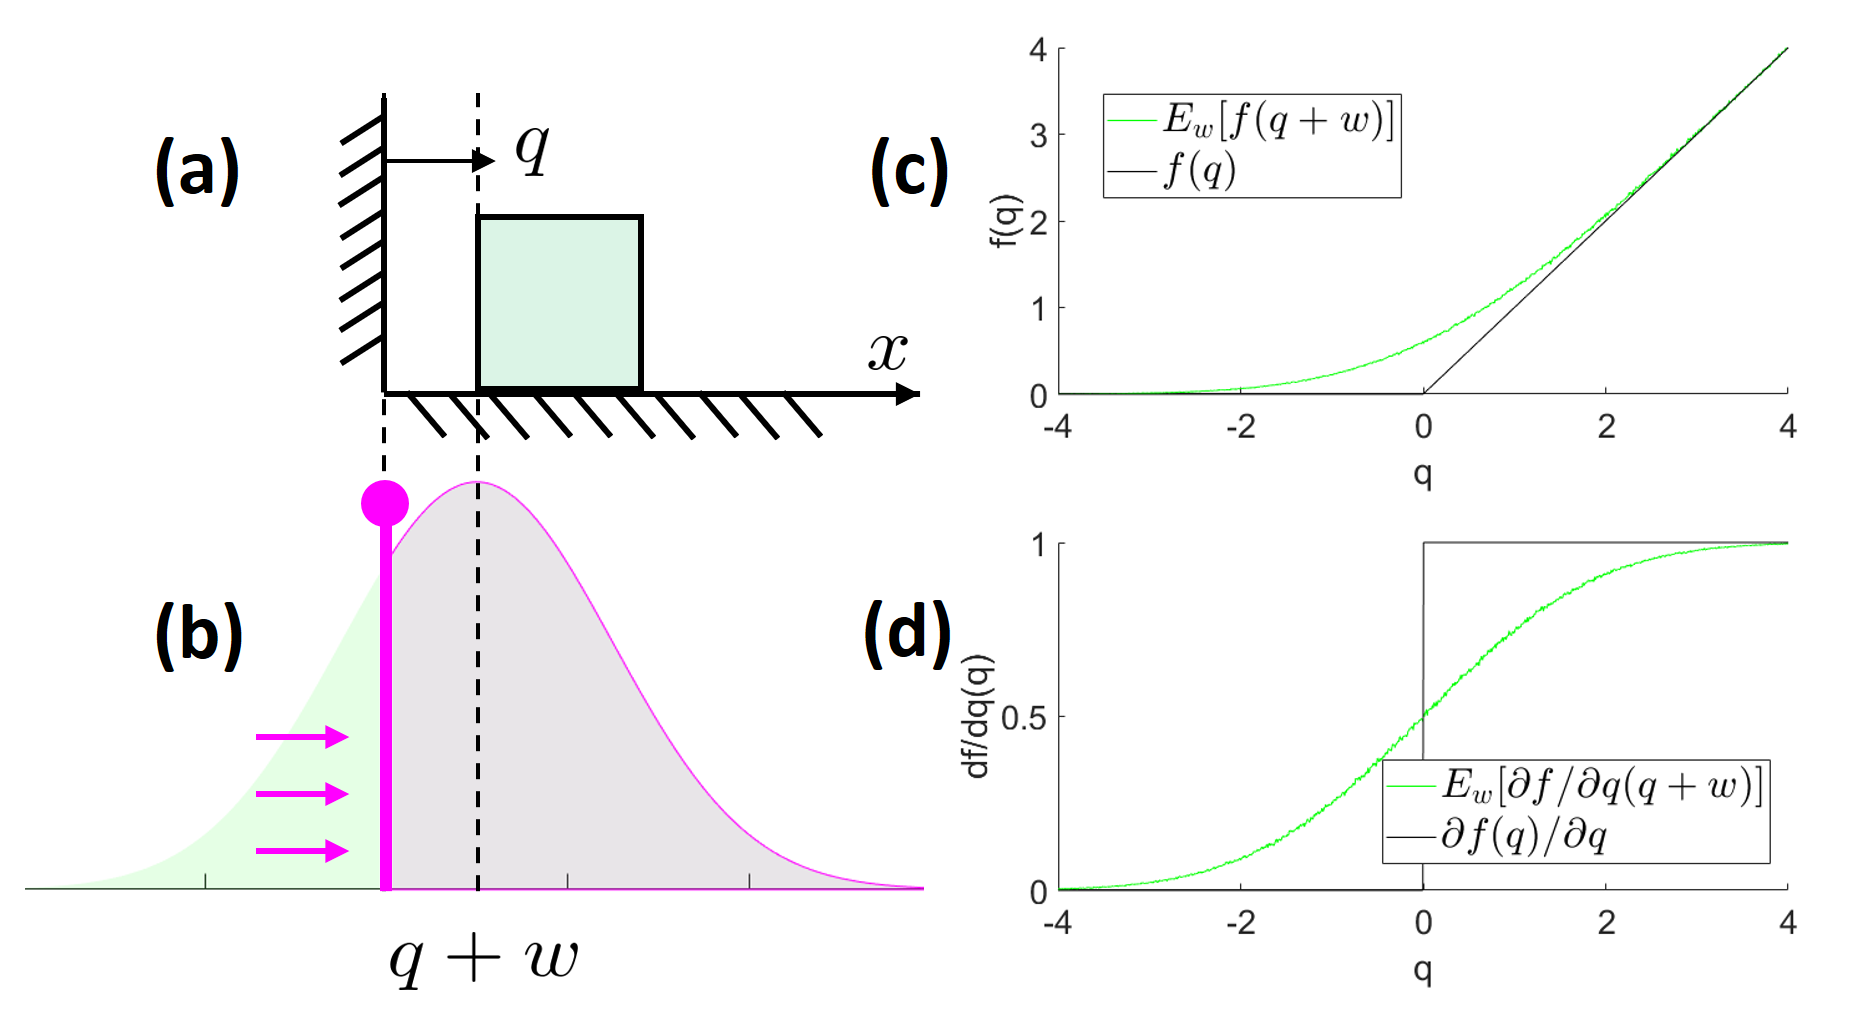
\includegraphics[width = 0.90\textwidth]{figures/02_quasi_static_dynamics/projection.png}
\caption{Figure for Example \ref{ex:projection}, where quasi-dynamics of motion is interpreted as a projection operator. (\textbf{a}) Illustration of the system. (\textbf{b}) Distribution of $q + w$ (green) and $f(q + w)$ (pink). Note that the samples for which $q+w_i<0$ have been projected onto the surface into a delta function, and the expectation of the pink distribution lies on the right side of $q$, creating a stochastic force field effect. (\textbf{c}) CQDC dynamics and its randomized smoothed version. (\textbf{d}) Gradients of the CQDC dynamics obtained with first-order randomized smoothing.}
\label{fig:projection}
\end{figure}
\end{example}

\subsection{A Smoothed Contact Dynamics Model}\label{sec:analyticsmoothing}
Both randomized smoothing schemes only involve repeatedly solving the CQDC dynamics \eqref{eq:q_dynamic_socp} and/or its gradient \eqref{eq:q_dynamics_AB}. In contrast, analytic smoothing (Sec.\ref{sec:smoothdynamics}) of the CQDC dynamics \eqref{eq:q_dynamic_socp} is not as straightforward, since the solution to an optimization problem does not give easy access to explicit forms from which we can analytically design smooth surrogates.

To perform analytic smoothing,  we can convert the hard constraints in a convex program into costs using a penalty method. Specifically, we convert the constrained program \eqref{eq:q_dynamic_socp} into an unconstrained convex program using the log-barrier function, a common technique in the interior-point method for convex conic programs, with weight $\kappa$:
\begin{equation}
\label{eq:q_dynamics_log}
\underset{\dq}{\minimize} \; \frac{1}{2} \dq^\intercal \mathbf{Q} \dq + b^\intercal \dq - \frac{1}{\kappa} \sum_{i=1}^{\nC} \log \left[\frac{(\Jn[i] \dq + \phi_i)^2}{\mu_i^2} - (\Jt[i]\dq)^\intercal \Jt[i]\dq \right],
\end{equation}
whose solution converges to the solution of \eqref{eq:q_dynamic_socp} as $\kappa \rightarrow \infty$ \cite[\textsection 11.3 and \textsection 11.6]{boyd2004convex}.

From a contact mechanics perspective, the log-barrier formulation is motivated by relaxing the strict complementary slackness condition of the CQDC dynamics to allow contact forces at a distance. In fact, the optimality conditions of \eqref{eq:q_dynamics_log} are almost identical to the KKT conditions of \eqref{eq:q_dynamic_socp}. The only difference is that complementary slackness \eqref{eq:friction_constraints:complementary_slackness} is relaxed from $v_i^\intercal \lambda_i = 0$ to $v_i^\intercal \lambda_i = \kappa^{-1}$ by the log barrier formulation ($v_i$ is defined in \eqref{eq:friction_constraints:v_i}).

The log-barrier term in \eqref{eq:q_dynamics_log} can be interpreted as the potential of a force field whose strength is inversely proportional to the distance to the boundary of the constraint \cite[p.567]{boyd2004convex}. For moderate values of $\kappa$, constraints can exert forces even though they are not active, achieving a smoothing effect similar to the ``force-at-a-distance'' relaxation of complementarity constraints, which are commonly used in planning through contact methods such as \cite{posa2014direct, howell2022dojo}. We will further illustrate this similarity in Example \ref{ex:equivalence}.

From $\dq^\star$, the solution to the smoothed dynamics \eqref{eq:q_dynamics_log}, we can directly compute the smoothed gradient $\A_\rho$ and $\B_\rho$ in the same way as \eqref{eq:q_dynamics_AB}. Once again, the derivatives of $\dq^\star$ with respect to $q$ and $u$ are computed by applying the implicit function theorem to the optimality condition of \eqref{eq:q_dynamics_log}, which only consists of the stationarity condition due to the absence of conic constraints.

To solve \eqref{eq:q_dynamics_log}, we implemented an in-house solver using Newton's method \cite[\textsection 9.5]{boyd2004convex}, and find that our out-of-the-textbook implementation works robustly and reliably for all numerical experiments in Sec. \ref{sec:traj_opt} and \ref{sec:rrt_results}.


\subsection{The Smooth Contact Model as ``Analytic Smoothing''} \label{sec:smoothing_equivalence}
In Sec. \ref{sec:smoothdynamics}, we saw that randomized and analytic smoothing can be interpreted as different methods of computing an equivalent quantity. Here, we show with examples that (\textbf{i}) for simple systems, we can derive the sampling distribution $\rho$ needed to obtain the smoothing given by the log-barrier-based analytic smoothing scheme; (\textbf{ii}) for more complex systems, randomized smoothing schemes using a Gaussian $\rho$ and the log-barrier-based analytic smoothing scheme result in qualitatively-similar smoothed dynamics.

\begin{example}\label{ex:equivalence} \normalfont(\textbf{Equivalence of Smoothing Schemes})
We start with the 1D frictionless system in Fig. \ref{fig:equivalence}a, whose dynamics is an instance of the frictionless CQDC dynamics \eqref{eq:q_dynamic_socp}:
\begin{equation}
\label{eq:q_dynamics_1d_cart}
\begin{aligned}
\underset{\dqa}{\minimize} \; &\frac{1}{2} hk_a (\dqa)^2 - h \ka (u - \qa) \dqa, \; \text{subject to} \\
&\qa + \dqa \geq 0,
\end{aligned}
\end{equation}

The KKT conditions of \eqref{eq:q_dynamics_1d_cart} are also the equations of motion of the system:
\begin{subequations}
\label{eq:wallcartdynamics}
\begin{align} 
h k_\mathrm{a} \left(\qa + \dqa - u\right) &= \lambda, \\
0 \leq \left(\qa + \dqa  \right) &\perp \lambda \geq 0,
\end{align}
\end{subequations}
which has the explicit solution
\begin{equation}
    q^\mathrm{a}_+ = \qa + \dqa =  \begin{cases}
        u & \text{ if } u \geq 0  \text{ (no contact) }\\
        0 & \text{ else } \text{ (contact) }\\
    \end{cases}.
\end{equation}

Also as an instance of \eqref{eq:q_dynamics_log}, \eqref{eq:q_dynamics_1d_cart} can be smoothed analytically by converting the constraint into a cost using the log-barrier function:
\begin{equation}
\underset{\dqa}{\minimize} \; \frac{1}{2} hk_a (\dqa)^2 - h \ka (u - \qa) \dqa - \frac{1}{\kappa} \log \left(\qa + \dqa \right),    
\end{equation}
whose optimality condition is obtained by setting the gradient of the smoothed cost to 0, yielding the equations of motion of the smoothed system: 
\begin{equation}
\label{eq:smooth_1d_cart}
hk_\mathrm{a}(\qa + \dqa - u) = \frac{1}{\kappa}\bigg(\frac{1}{\qa + \dqa}\bigg).
\end{equation}

The right-hand side of \eqref{eq:smooth_1d_cart} can be interpreted as an impulse whose magnitude is inversely proportional to the distance to the wall. Calling this impulse $\beta$, we note that
\begin{equation}
\label{eq:complementarity_simple}
    \beta (\qa + \dqa) = \kappa^{-1},
\end{equation}
which is analogous to the common bilinear relaxation to the complementarity constraint for contact \cite{posa2014direct, howell2022dojo}\footnote{
In trajectory optimization, the complementarity constraint is usually relaxed to $\beta (\qa + \dqa) \leq \kappa^{-1}$, instead of the equality in \eqref{eq:complementarity_simple}. The inequality gives the constraint non-empty interior, making it numerically better.
}.

The solution to \eqref{eq:smooth_1d_cart} is given by 
\begin{equation}
    q^\mathrm{a}_+=\frac{1}{2}\left(u + \sqrt{u^2 + \frac{4}{\kappa h^2k^2_\mathrm{a}}}\right)
\end{equation}
which is equivalent to randomized smoothing of the original dynamics under the following elliptical distribution
\begin{equation}
    \rho(w) = \sqrt{\frac{4\sigma }{(w^\intercal\sigma w + 4)^3}},
\end{equation}
where $\sigma\coloneqq hk\kappa $.
\end{example}

Conversely, we hypothesize the existence of a barrier function that corresponds to the Gaussian density, though its form is prohibitive for analysis. In addition, for more complex examples involving friction, such as the system in Fig. \ref{fig:equivalence}b, obtaining an analytic expression for $\rho$ when the contact dynamics is smoothed by log barrier \eqref{eq:q_dynamics_log} is difficult. Instead, we numerically illustrate the performance of the two smoothing schemes in Fig. \ref{fig:equivalence}e. More details about this example can be found in \cite{bundledgradients}.
\begin{figure}
\centering
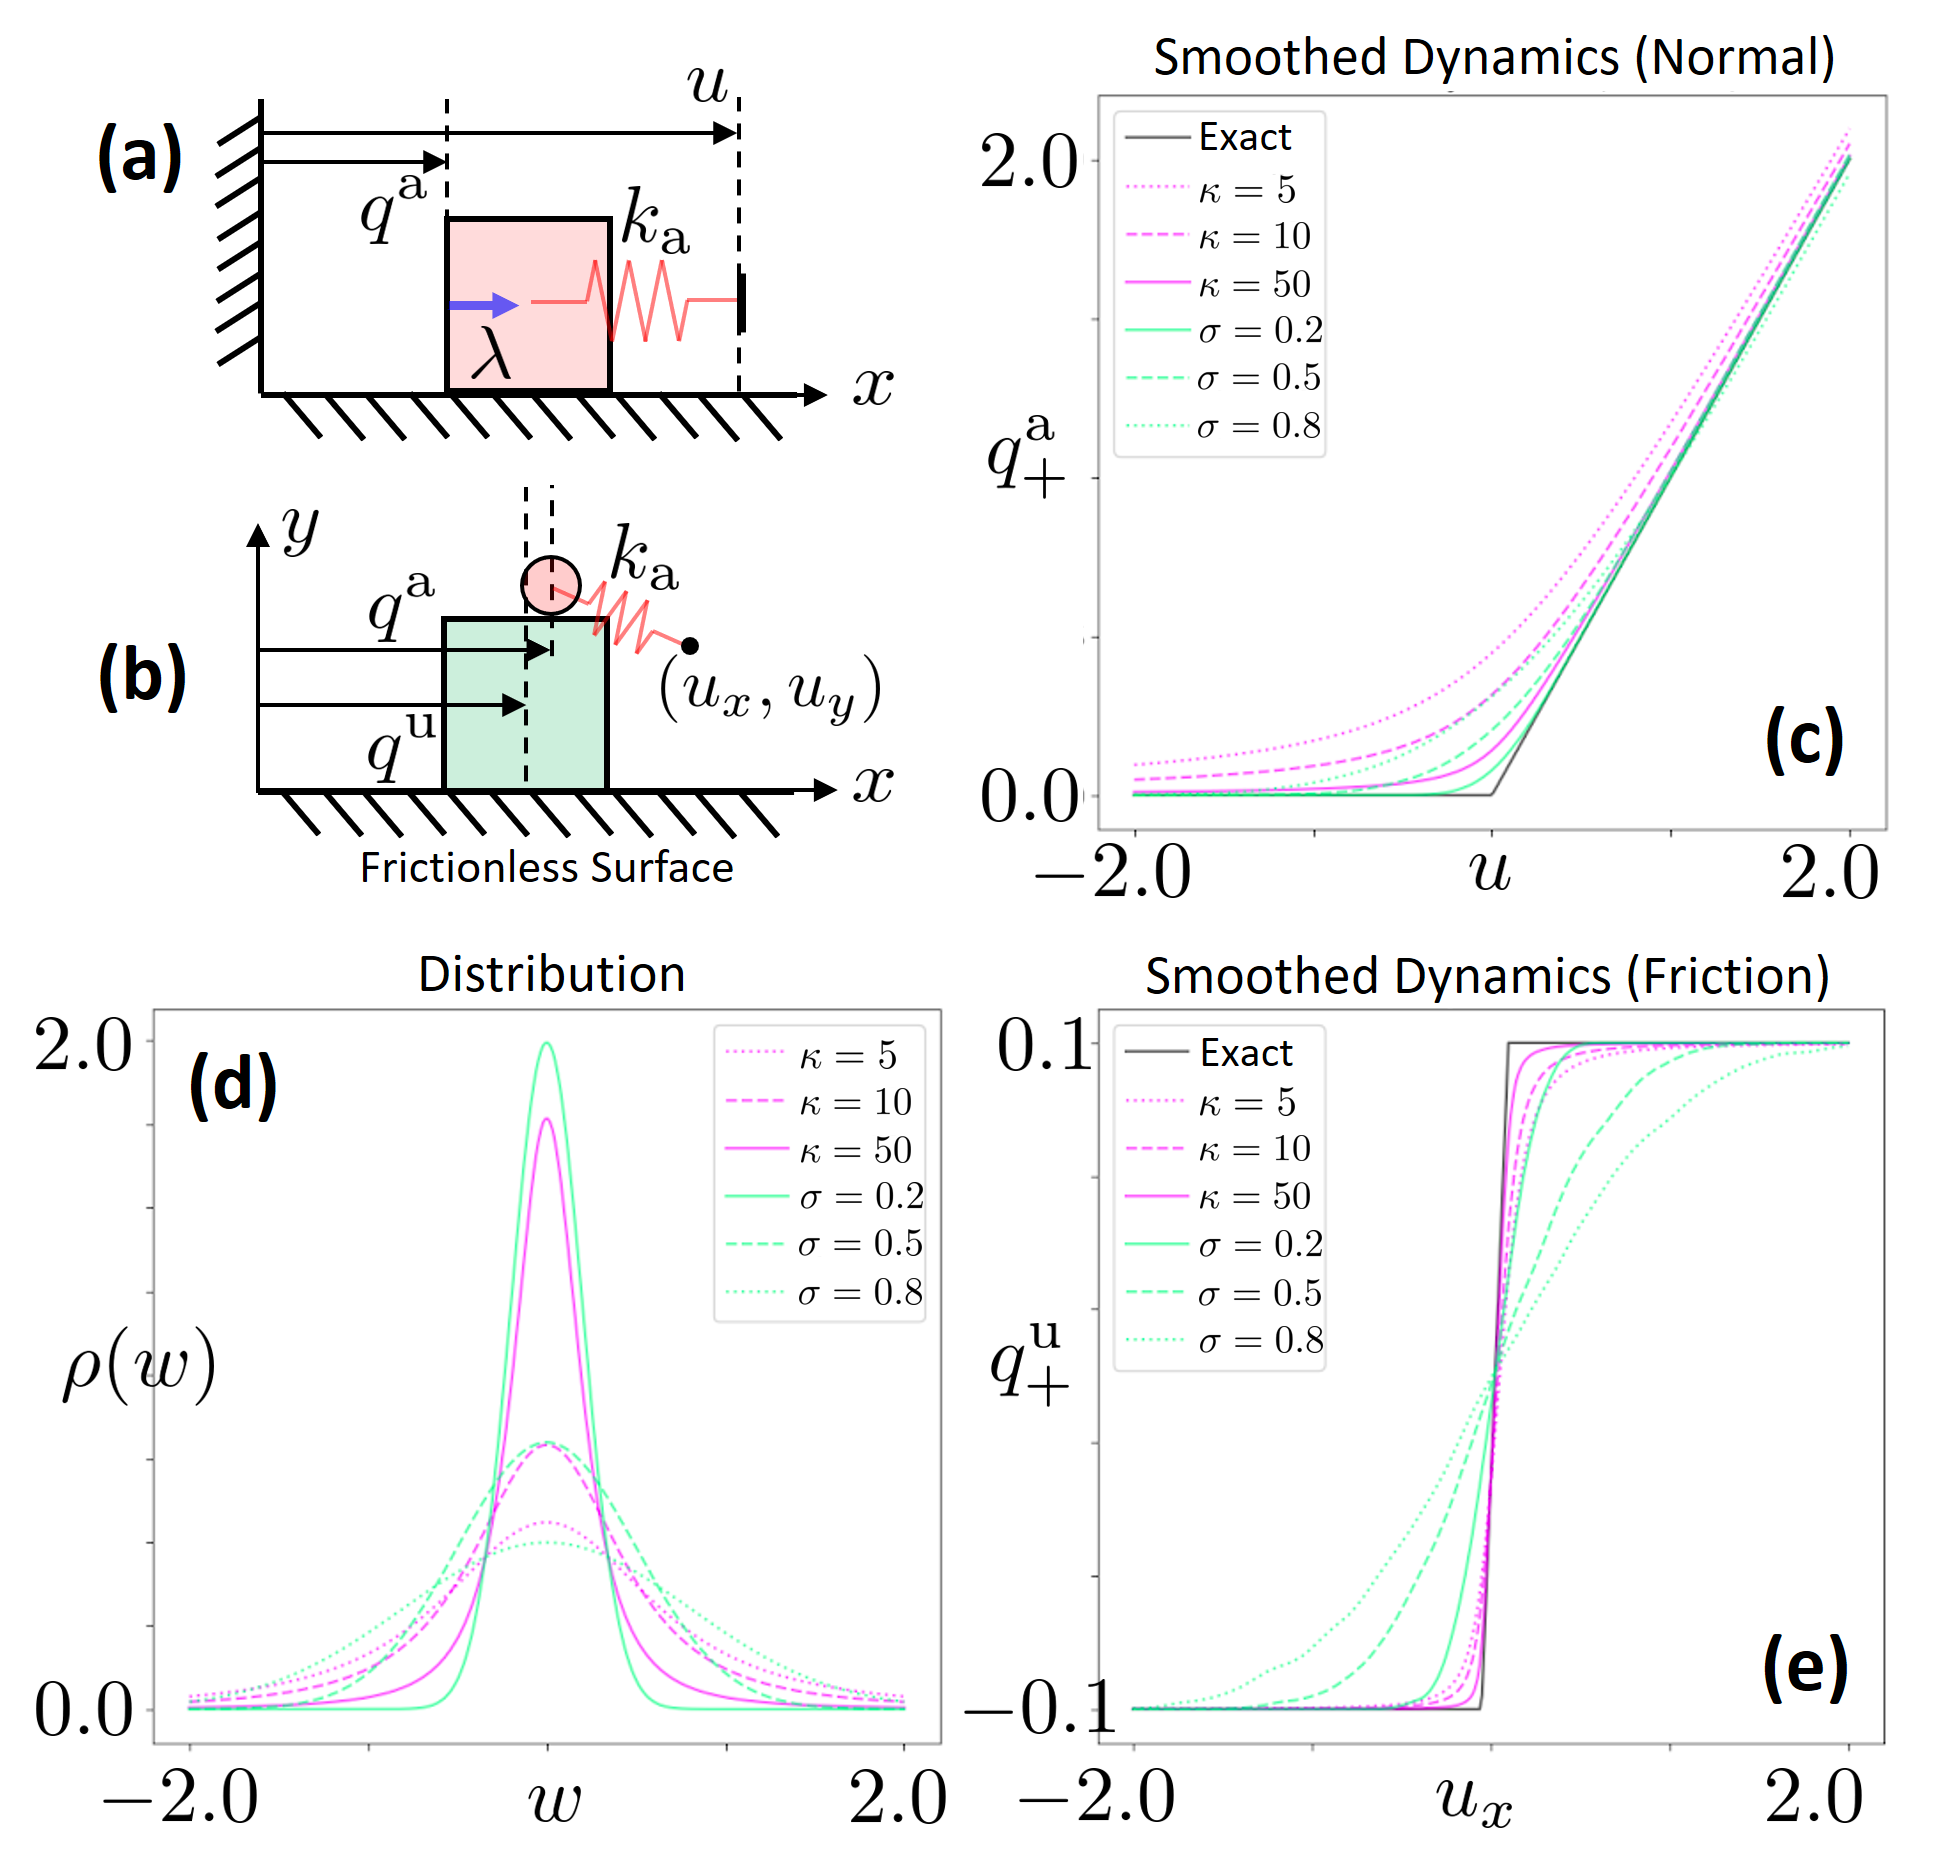
\includegraphics[width = 0.90\textwidth]{figures/02_quasi_static_dynamics/equivalence.png}
\caption{
(\textbf{a}) A system consisting of an actuated cart constrained to slide on a frictionless surface, and a wall occupying $\qa \leq 0$. The actuator has stiffness $k_\textrm{a}$.
(\textbf{b}) A system consisting of an un-actuated cart constrained to slide on a frictionless surface, and a ball actuated along both the $x$ and $y$ axes. The ball can touch the top surface of the cart with a frictional contact.
(\textbf{c}) Randomized and analytic smoothing of (a). Randomized smoothing, shown in green, is done with a Gaussian kernel with different variances $\sigma$. Analytic smoothing, shown in magenta, is done with different log-barrier weights $\kappa$. 
(\textbf{d}) Density functions of the Gaussian kernels (green) and the elliptical distributions used for analytic smoothing (magenta). 
(\textbf{e}) Randomized and analytic smoothing of (b). We plot $q^\mathrm{u}_+$ against $u_x$ for a fixed $u_y$ that is inside the cart. The linear region in the plot corresponds to sticking contact, and the flat regions to sliding.}
\label{fig:equivalence}
\end{figure}


Finally, we note that with a different smoothing scheme which relaxes complementary slackness, Howell \textit{et al.} showed a similar trend for the smoothed dynamics as the relaxation is tightened \cite[Fig. 7]{howell2022dojo}. We believe this corroborates the equivalence between analytic and randomized smoothing schemes.


\chapter{Contact-Rich Manipulation Planning using Quasi-static Models} \label{chapter:contact_rich_planning}
\section{Introduction}
In Chapter 2, we have developed the CQDC dynamics and prposed computational methods to obtain local linear models of its smooth surrogate. These tools are not specific to any algorithm: they can improve the performance of most iterative planning algorithms that rely on local approximations. 

We start the section on contact-rich planning with iterative MPC (iMPC) \cite{bundledgradients}, a variant of trajecotry optimization, that uses the CQDC dynamics to enforce contact dynamics constraints and compute smoothed gradients. In addition to demonstrating the utility of the proposed CQDC dynamics, we also introduce iMPC as a handy refinement tool for trajectories generated by SBMP. Such trajectories are well-known for making inefficient and meandering ``dances'' before arriving at the goal. 

However, we have argued that the success of contact-rich planning depends on both smoothing and global search. Planning based on local optimization, including trajectory optimization with smoothed contact dynamics, generally results in non-convex optimization problems where the quality of different local minima can be a make-or-break factor. Solving such problems requires non-trivial initialization and cost tuning \cite{onol2020tuning}, both of which can be highly problem specific and notoriously hard to debug. This motivates us to search further for a more global approach.

In robotics, SBMP algorithms such as the Rapidly-Exploring Random Tree (RRT) \cite{lavalle1998rapidly} are widely used for global search problems, including those with kinodynamic constraints \cite{karaman2010optimal}. However, the success of such planners has rarely extended to contact-rich settings. We find that while optimization-based methods for planning through contact have employed smoothing schemes, all existing SBMP methods for contact planning explicitly consider modes instead of smoothing them \cite{cheng2021contact,wu2020r3t,chen2021trajectotree,motioncones,terry}, as SBMP methods do not inherently require local characterizations of dynamics (i.e. gradients). Yet, previous works have shown that such local models are highly relevant for designing more efficient distance metrics during the nearest neighbor queries that respects dynamic reachability \cite{shkolnik2009reachability,wu2020r3t,haddad2021anytime}.

In this chpater, we fill in this gap by combining contact mode abstraction via smoothing, and the global search capabilities of RRT. We enable RRT to explore efficiently through contact constraits by utilizing a novel distance metric based on the local smoothed linearizations of CQDC dynamics (Sec.\ref{sec:mahalanobis}). In addition, we further propose an efficient extension step by computing actions that expand the tree to new parts of the state-space using the local linearizations (Sec.\ref{sec:rrt_for_contact}). With a variety of contact-rich tasks inspired by \cite{rajeswaran2018learning} that involve both intrinsic and extrinsic dexterity \cite{extrinsic}, we show that combining smoothing with RRT achieves tractable global motion planning for highly contact-rich manipulation (Sec.\ref{sec:rrt_results}); and that the planned trajectories can transfer to high-fidelity second-order simulations or even robot hardware. To the best of our knowledge, our work appears to be the first to successfully combine SBMP with contact mode smoothing.

\section{Trajectory Optimization through Contact \label{sec:traj_opt}}
\noindent 
In this section, we demonstrate the efficacy of smoothed CQDC dynamics on trajectory optimization for systems with contacts.
Although smoothing of hard contact constraints has been widely utilized to improve convergence \cite{posa2014direct, howell2022dojo, howell2022trajectory}, existing methods still struggle with complex problems such as dexterous manipulation. In particular, the quality of solutions can be very sensitive to initial guesses \cite{onol2020tuning}.
In this context, we show that a variant of trajectory optimization, with the help of smoothed CQDC dynamics and only a trivial initial guess, can perform well even on dexterous manipulation tasks.

\subsection{Iterative MPC with Smoothing \label{sec:iMPC}}
The variant of trajectory optimization algorithm used in this section, which we call iterative MPC (iMPC), is an iLQR-inspired algorithm proposed in \cite{bundledgradients}. We briefly summarize iMPC here for completeness, and illustrate how smoothing can be easily integrated into iMPC.

Consider the problem of finding an optimal sequence of inputs to track some desired state trajectory $\{x^d_t\}_{t=0}^T$. We need an initial guess for the nominal input trajectory $\{\bar{u}_t\}^{T-1}_{t=0}$, from which the nominal state trajectory $\{\bar{x}_t\}^T_{t=0}$ can be obtained by rolling out $\{\bar{u}_t\}^{T-1}_{t=0}$ from the initial state $x_0$. For every time $t$ (i.e. in a time-varying manner), we can create a locally linear model that approximates the dynamics, with model parameters $\{\mathbf{A}_t,\mathbf{B}_t,c_t\}_{t=0}^{T-1}$ \eqref{eq:linearization}. Then, finding the optimal $\{\bar{u}_t\}^{T-1}_{t=0}$, subject to the locally linear model of the dynamics, can be written as a QP. We present the MPC variant of this problem that receives the initial state $\bar{x}_j$ at time $t=j$ and computes the optimal action for the remaining time steps,
\begin{subequations}
\label{eq:trajopt}
\begin{align}
\textbf{MPC}(\bar{x}_j) & = u^\star_j, \text{where}\\
\min_{x_t,u_t}\;\; & \norm{x_T-x_T^d}_{\mathbf{Q}_T}^2 + \sum^{T-1}_{t=j} \left(\|x_t - x^d_t\|^2_{\mathbf{Q}_t} + \|u_t\|^2_{\mathbf{R}_t}\right)\\
\text{s.t.}\;\; & x_{t+1} = \mathbf{A}_t(x_t-\bar{x}_t) + \mathbf{B}_t(u_t - \bar{u}_t) + c_t,\\
& \mathbf{C}^x_t x_t\leq d^x_t,\; \mathbf{C}^u_t u_t \leq d^u_t, \; \forall t\in\{j \cdots T-1\},\\
& x_j = \bar{x}_j.
\label{eq:trajopt:x_u_constraints}
\end{align}
\end{subequations}

Here, $\{\mathbf{Q}_t,\mathbf{R}_t\}$ are the quadratic weights for state and input, respectively; $\mathbf{Q}_T$ is the weight on the terminal state; $\{\mathbf{C}^x_t,d^x_t\}$ and $\{\mathbf{C}^u_t,d^u_t\}$ are inequality parameters on the state and input, respectively. The linear constraints \eqref{eq:trajopt:x_u_constraints} can enforce, for instance, joint and actuation limits.

The iMPC algorithm is summarized in Alg. \ref{alg:impc}. 
In every outer iteration (body of the $\mathtt{while}$ loop starting at Line \ref{alg:impc:while}), iMPC solves truncated versions of \eqref{eq:trajopt} for $T - 1$ times. Specifically, at inner iteration $j$ (body of the $\mathtt{for}$ loop starting at Line \ref{alg:impc:for}), we solve MPC \eqref{eq:trajopt} for the sub-problem starting at $t=j$ (Line \ref{alg:impc:mpc}), and apply $u_j^\star$ from the solution to update $\bar{x}_{j+1}$ (Line \ref{alg:impc:update_x}). In every inner iteration, we also enforce a trust region by using \eqref{eq:trajopt:x_u_constraints} to constrain $x_t$ and $u_t$ to stay close to $\bar{x}_t$ and $\bar{u}_t$, respectively.

\begin{algorithm}
\caption{\textbf{iMPC}}\label{alg:impc}
\textbf{Input:} Initial state $x_0$, input trajectory guess $\{\bar{u}_t\}_{t=0}^{T-1}$\;
\textbf{Output:} Optimized input trajectory $\{\bar{u}_t\}_{t=0}^{T-1}$ \;
$\{\bar{x}_t\}_{t=0}^T\leftarrow$ Rollout $f$ from $x_0$ with$\{\bar{u}_t\}_{t=0}^{T-1}$\;
\While {\textrm{not converged}}{ \label{alg:impc:while}
    Compute system matrices $\{\mathbf{A}_t,\mathbf{B}_t,c_t\}_{t=0}^{T-1}$\;
    \For {$0\leq j < T$} { \label{alg:impc:for}
        $\bar{u}_j \leftarrow \mathbf{MPC}(\bar{x}_j)$ \label{alg:impc:mpc}\; 
        $\bar{x}_{j+1} \leftarrow f(\bar{x}_j,\bar{u}_j)$ \label{alg:impc:update_x}\;
    }
}
\algorithmicreturn $\; \{\bar{u}_t\}_{t=0}^{T-1}$
\end{algorithm}

To apply smoothing to iMPC, we substitute the linearizations of smooth surrogates $\{\mathbf{A}_{t,\rho},\mathbf{B}_{t,\rho},c_{t,\rho}\}^{T-1}_{t=0}$ \eqref{eq:ABc_rho} for the first-order Taylor expansions $\{\mathbf{A}_t,\mathbf{B}_t,c_t\}_{t=0}^{T-1}$ \eqref{eq:linearization}. After every outer iteration, we also reduce the variance of $\rho$ (this can be done for analytic smoothing by increasing the log barrier weight $\kappa$), allowing the smooth surrogates $f_\rho$ to converge to the true CQDC dynamics $f$.

\begin{figure*}
\centering
\subfloat[\code{PlanarPushing}.]{
	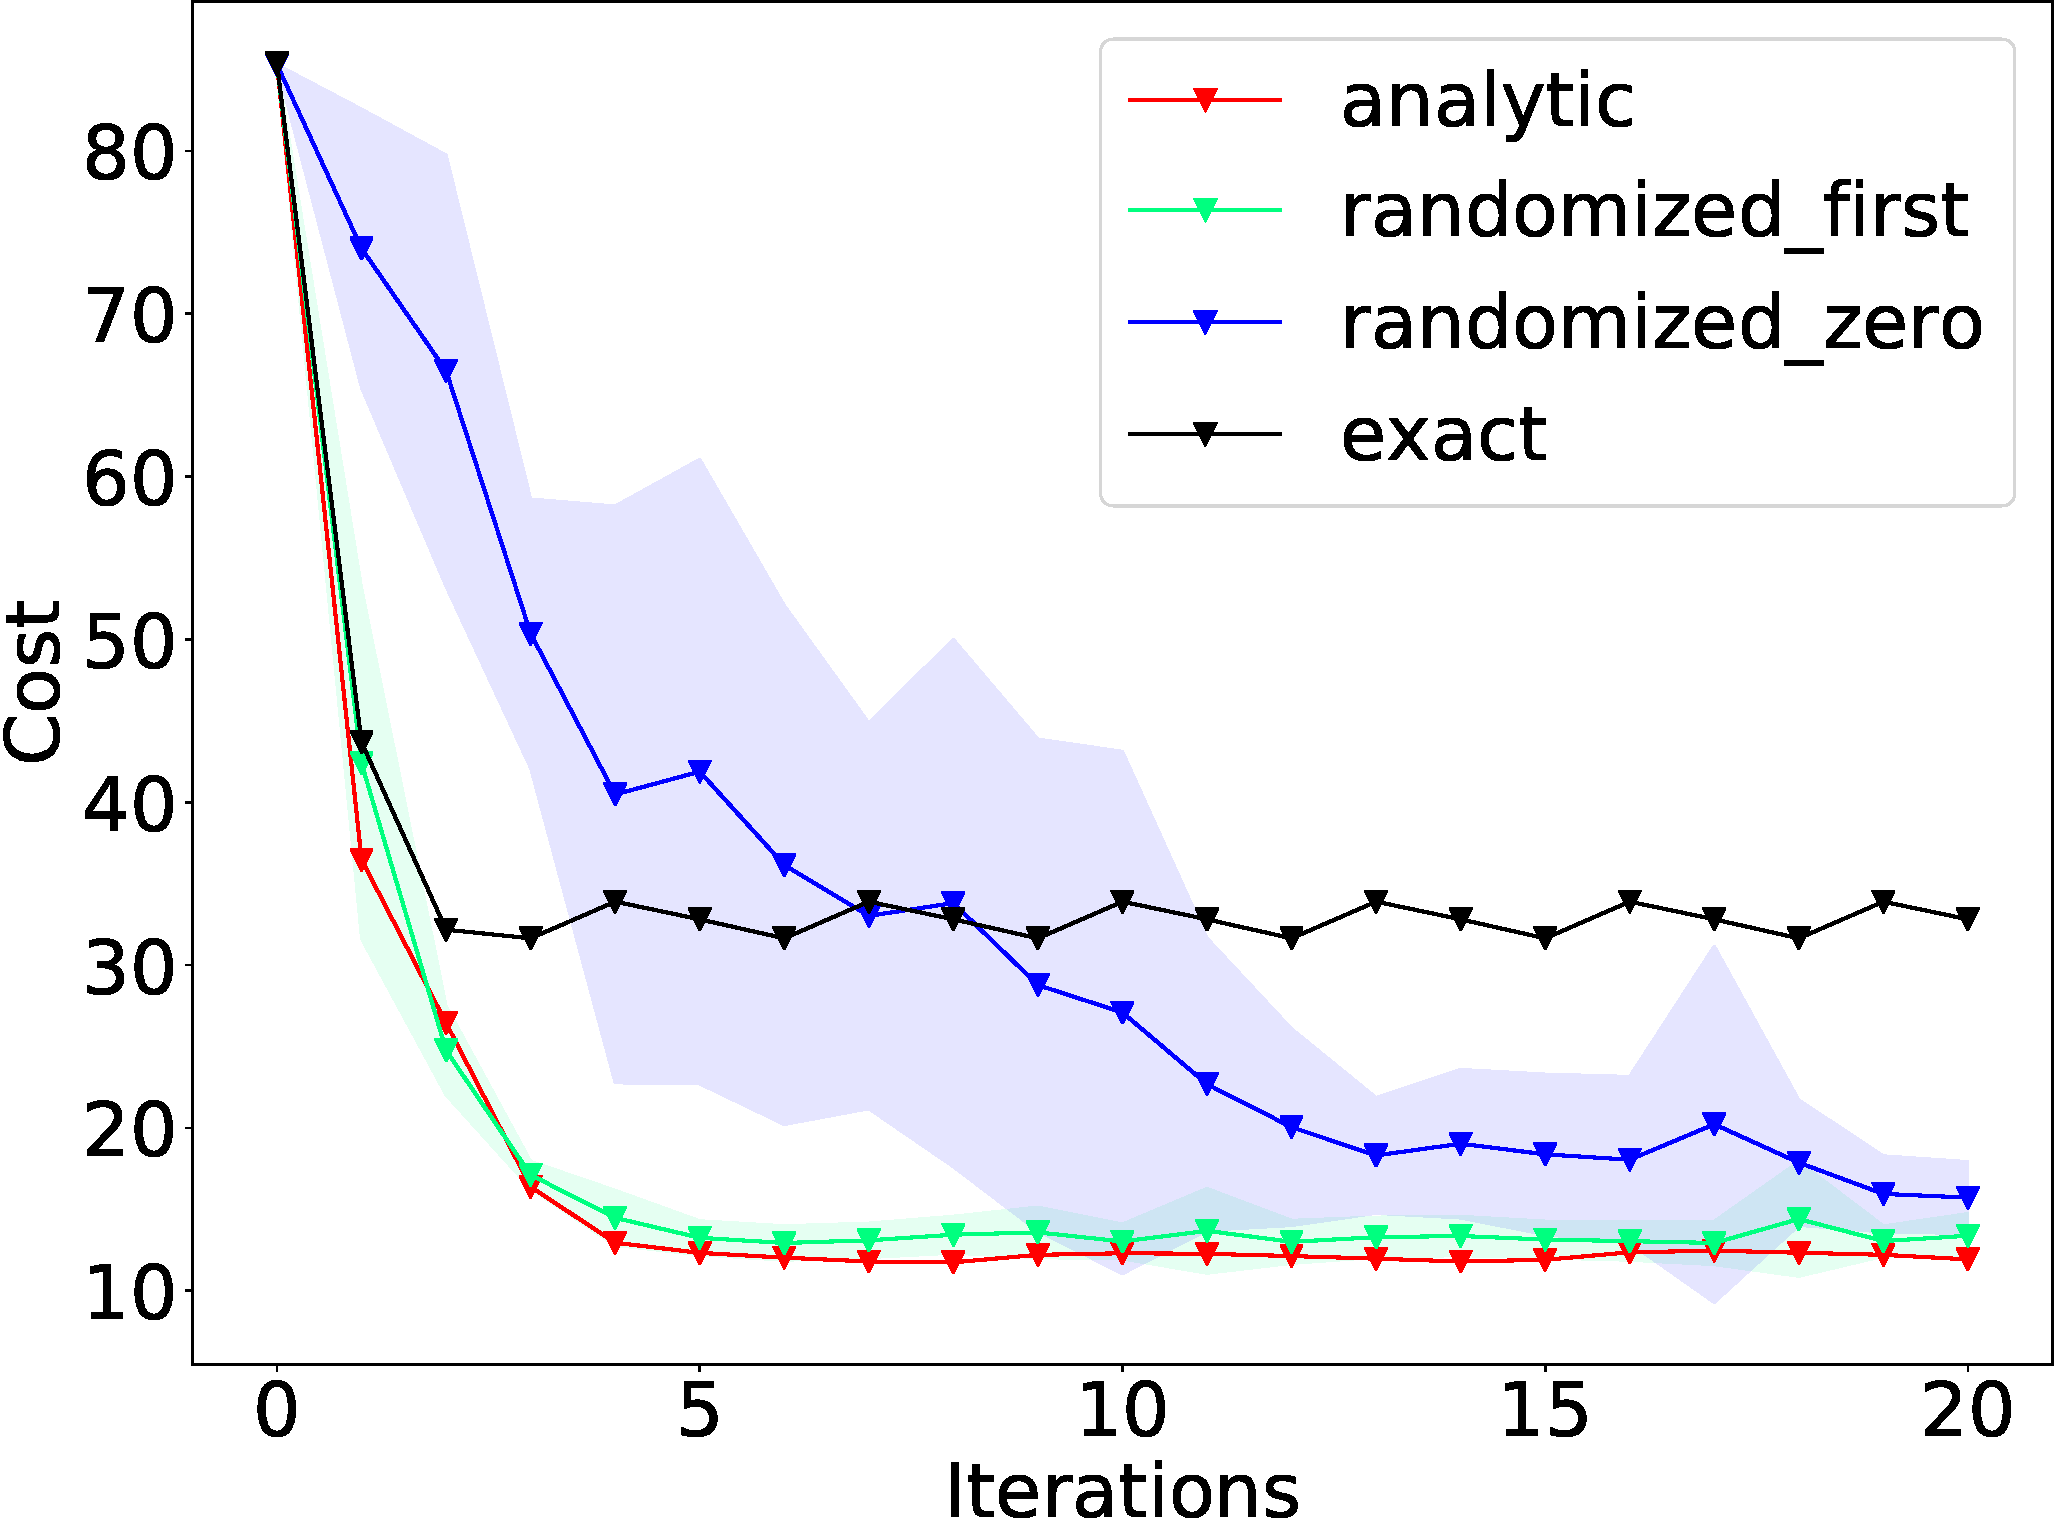
\includegraphics[width=0.32\linewidth]{figures/03_contact_rich_planning/trajopt_results/planar_pushing.pdf}
}
\subfloat[\code{PlanarHand} Re-orientation.]{
	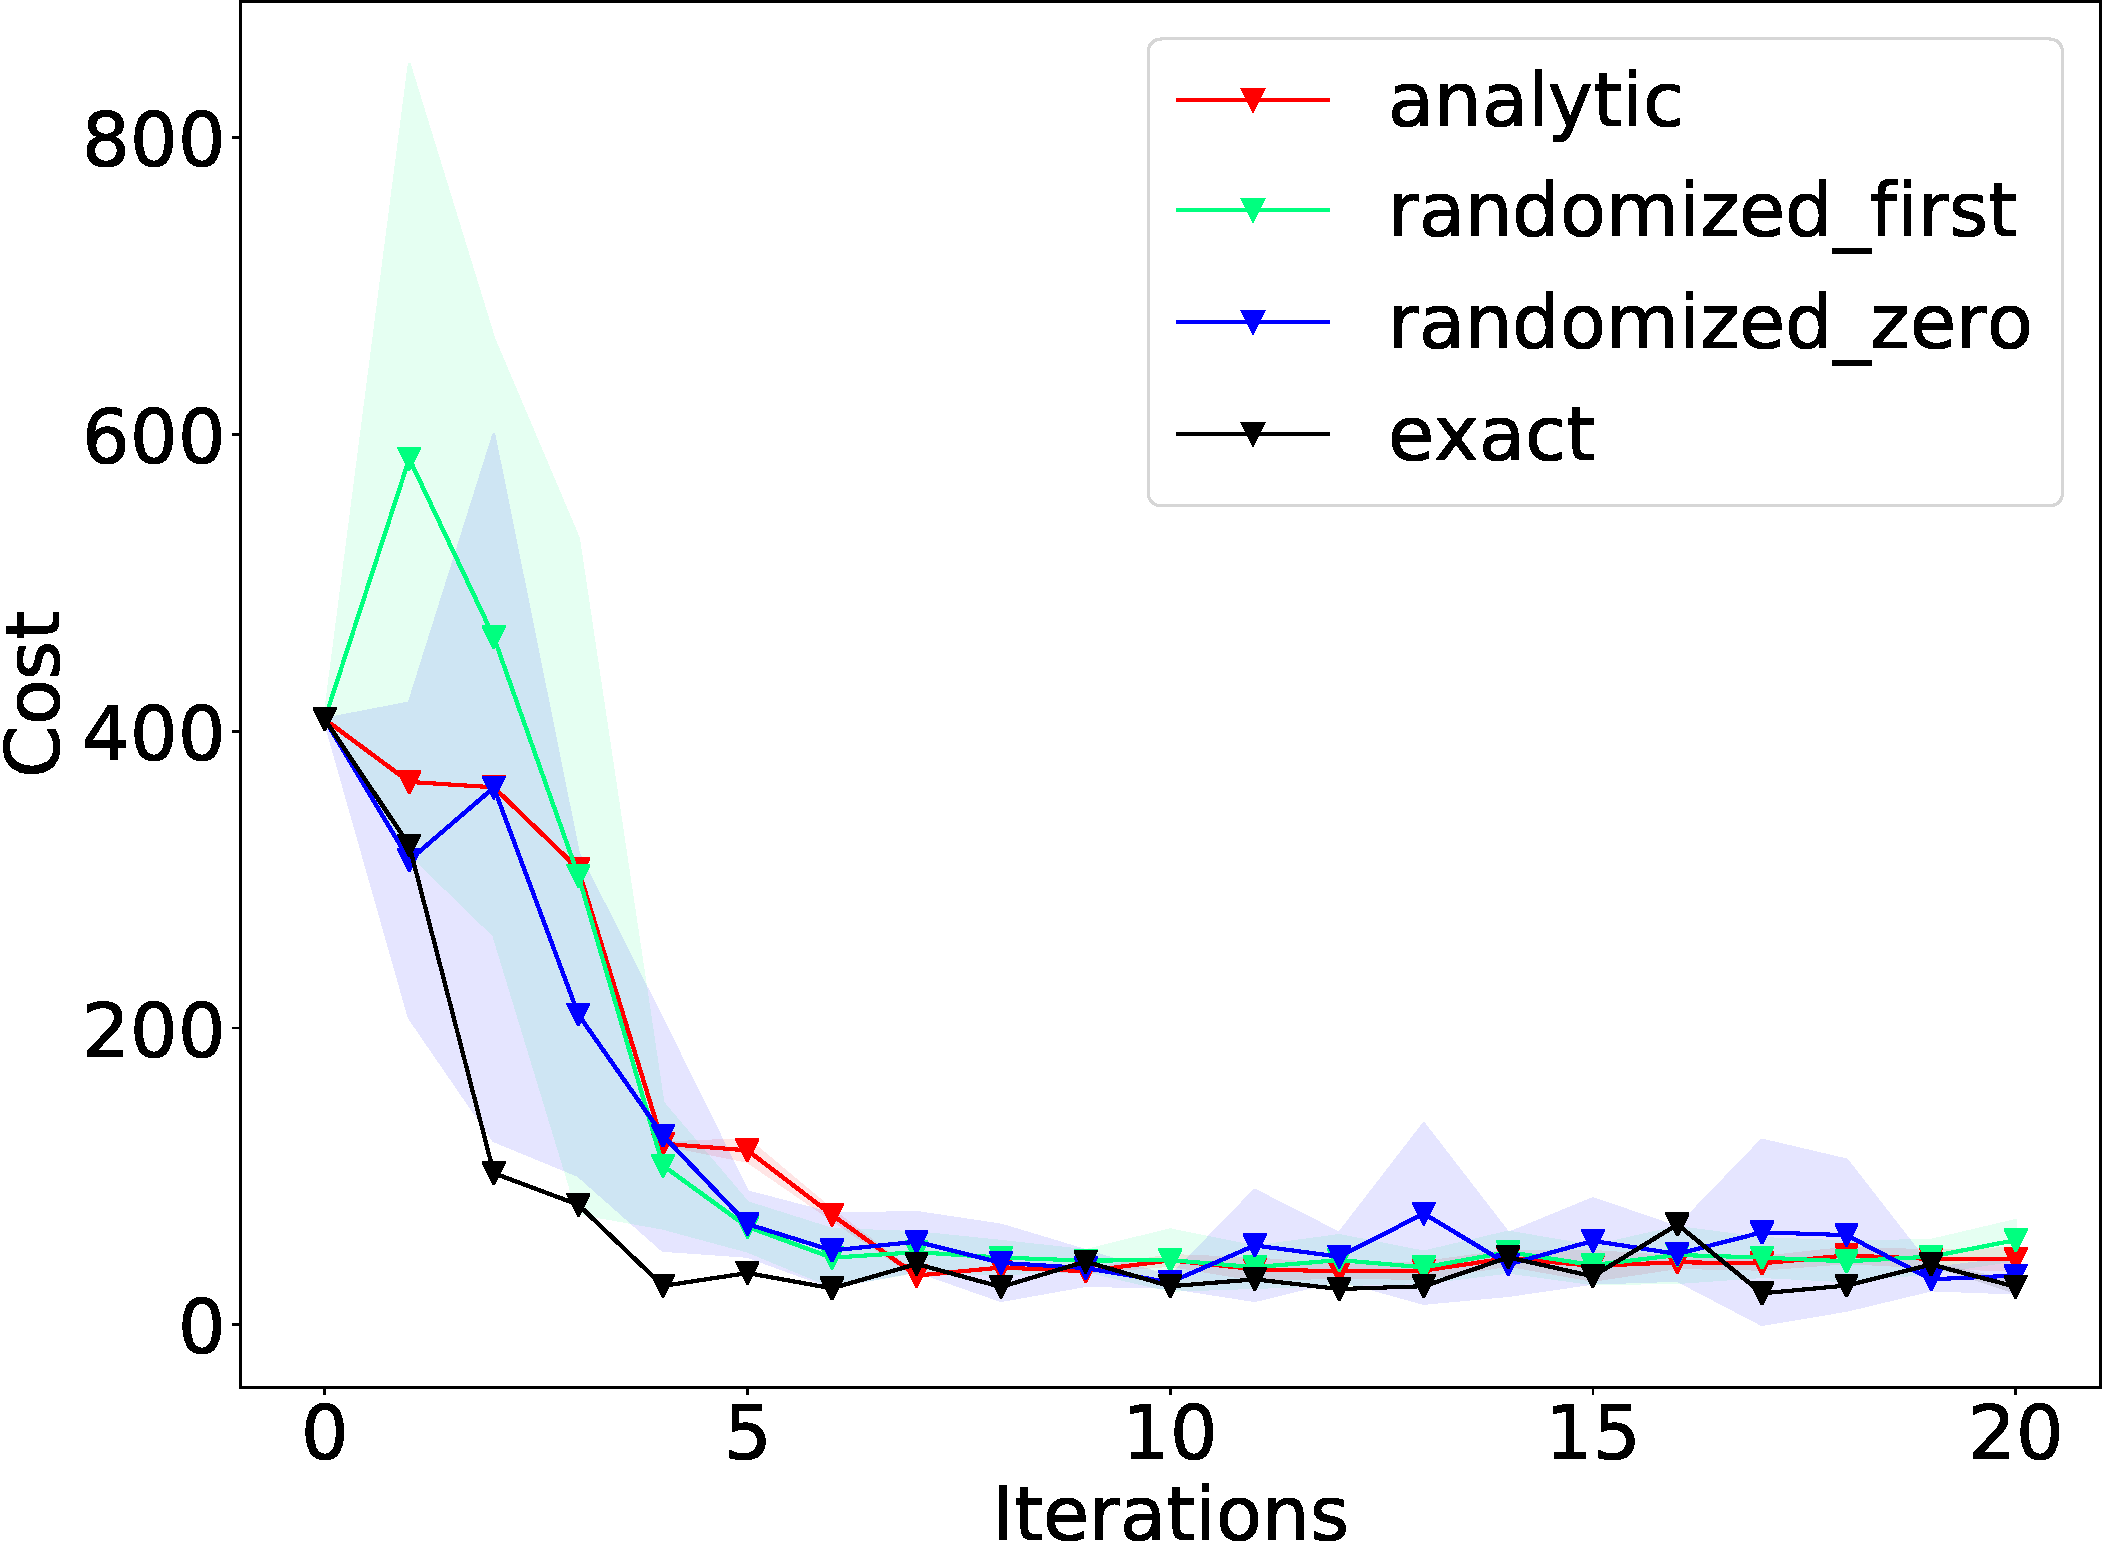
\includegraphics[width=0.32\linewidth]{figures/03_contact_rich_planning/trajopt_results/planar_hand.pdf}
}
\subfloat[\code{AllegroHand} Rotation.]{
	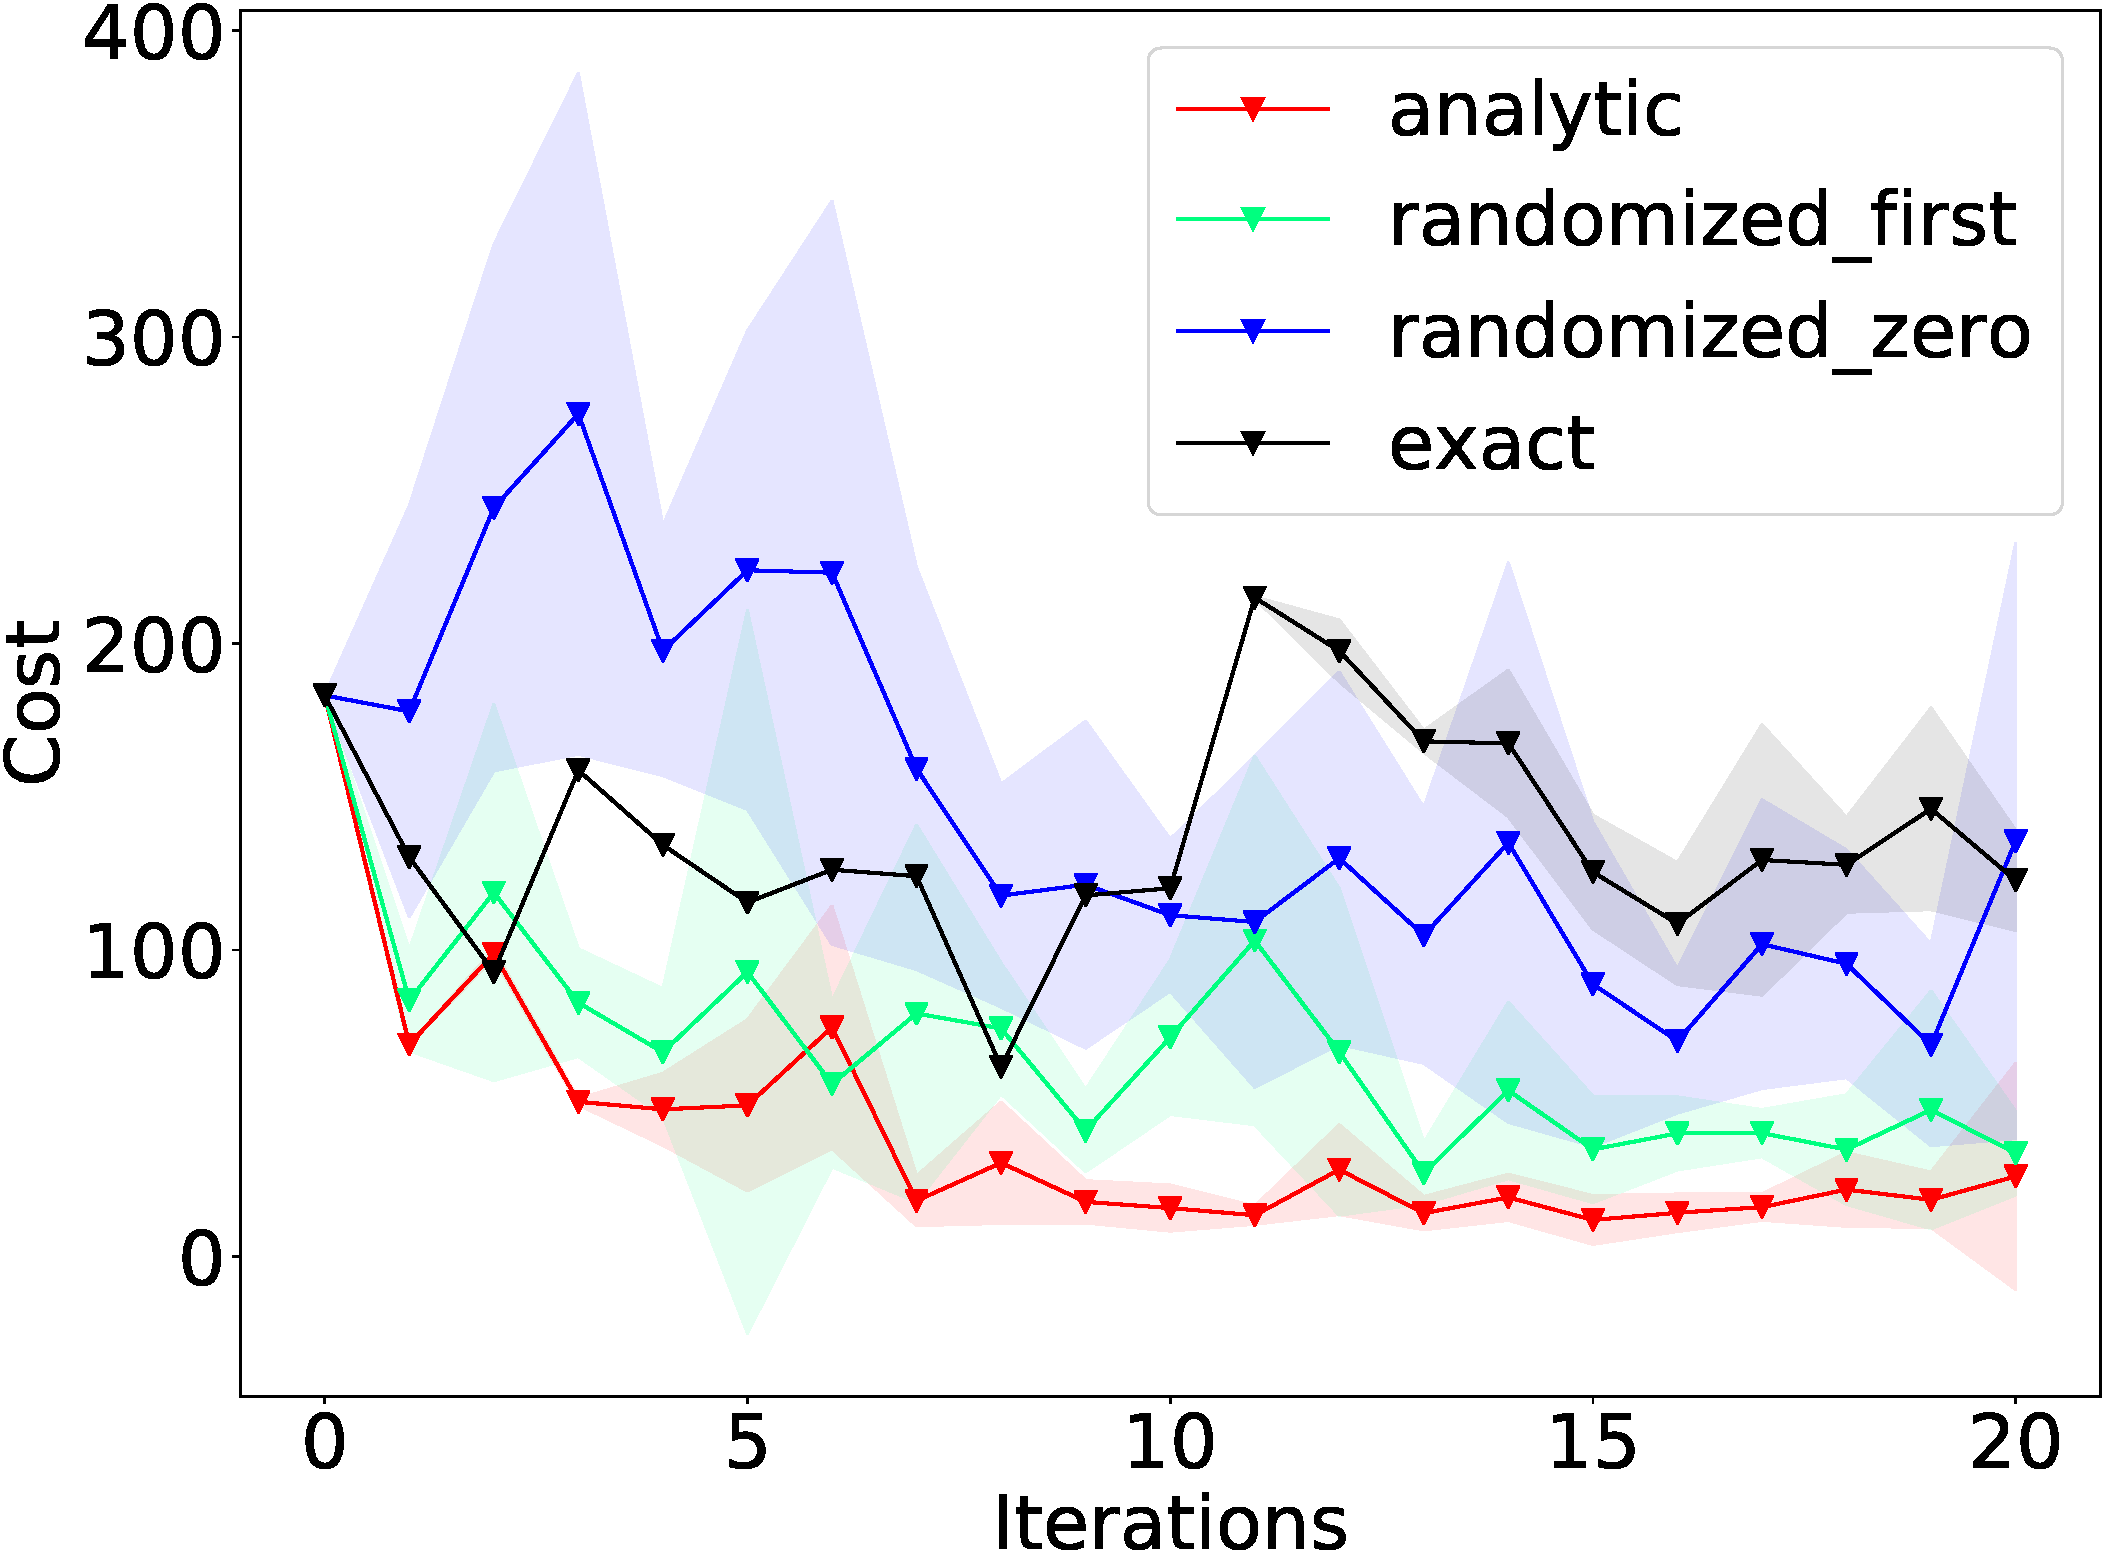
\includegraphics[width=0.32\linewidth]{figures/03_contact_rich_planning/trajopt_results/allegro_hand.pdf}
}
\caption{Performance of iMPC with different smoothing schemes: analytic, randomized (first-order), randomized zero-order, and exact (no smoothing). For each method, the solid line represents the mean over five runs, and the shaded region represents the standard deviation. }
\label{fig:trajoptperformance}
\end{figure*}

\subsection{Experiment Setup}\label{sec:trajopt_setup}
\subsubsection{Systems Description \label{sec:trajopt_setup:systems}}
We test iMPC with different smoothing schemes on two planar systems from \cite{bundledgradients} and a 3D system for in-hand rotation. We describe our systems below, and their visualization can be seen in Fig. \ref{fig:rrtperformance}. The three tuple after the name of each system indicates $(\nU, \nA, \nCG)$, where $\nU$ is the number of unactuated DOFs, $\nA$ the number of actuated DOFs, and $\nCG$ the number of collision geometries.

\begin{enumerate}
\item {\bf Planar Pushing, (3,2,2)}.  A classical example of nonprehensile manipulation \cite{lynch1996stable}. The goal is specified as some 2D configuration of the box.
\item {\bf Planar Hand Reorientation, (3,4,13)}.  We use a planar hand with two fingers, each with two DOFs. The goal is to change the position and orientation of the ball in a 2D plane.
% , the 2D robot pushes the object to desired position and orientation. 
\item {\bf Allegro In-Hand Rotation, (6,16,20)}.  3D In-hand rotation of the ball with the full model of the allegro hand \cite{huang2020efficient}. The goal is specified as a rotated configuration of the ball.
\end{enumerate}

\subsubsection{Initialization}
As mentioned in Sec. \ref{sec:iMPC}, given an initial state $x_0$, we need to initialize the nominal input trajectory $\{\bar{u}_t\}^{T-1}_{t=0}$, where $\bar{u}_t$ is the commanded positions of the robots at step $t$ under the CQDC dynamics. Empirically, we find that good convergence can be achieved with a constant initialization, i.e. $\bar{u}_0 = \bar{u}_1 = \dots \bar{u}_{T-1}$. Although this initialization is still prone to local minima, it is surprisingly effective when the solution can be found without global search.

For the numerical experiments in this section, we need a $\bar{u}_0$ that makes contact with the object. Otherwise the baseline which does not use smoothing would have zero gradients and make no progress at all. 

In contrast, for iMPC with smoothing, it is sufficient to set $\bar{u}_0 = q^\mathrm{a}_0$, as long as $q^\mathrm{a}_0$ is not ``too far away'' from making contact with the objects (the reason is explained in Example \ref{ex:planarhandreachableset}). In many practical problems, the object's initial configuration $q^\mathrm{u}_0$ is fixed, but we are free to choose the initial robot configuration $q^\mathrm{a}_0$. In this case, we can simply calculate a $q^\mathrm{a}_0$ that is ``close'' to making contact using, for example, methods that compute grasps \cite{murray2017mathematical}. 

\subsubsection{Hardware \& Implementation Details}
The numerical experiments are run on a desktop with one AMD Threadripper 2950 CPU (16 cores, 32 threads) and 32GB of RAM. The code for iMPC using different smoothing schemes is identical except for the computation of the linearizations. For analytic smoothing and the baseline, we solve respectively the smoothed \eqref{eq:q_dynamics_log} and original \eqref{eq:q_dynamic_socp} dynamics once and then apply the chain rule to get the linearization. For first-order randomized smoothing, we solve the original dynamics \eqref{eq:q_dynamic_socp} and apply the chain rule for 100 samples ($N=100$), which is parallelized on all available threads, and then average the gradients of the samples. Zeroth-order randomized smoothing simply requires parallel evaluation of the dynamics.


\begin{figure}[t]
\centering
\subfloat[Initial configurations and goals. Each system is shown in its initial configuration $q_0$. The thicker frame denotes the goal while the thinner frame denotes the initial configuration of the object.]{
	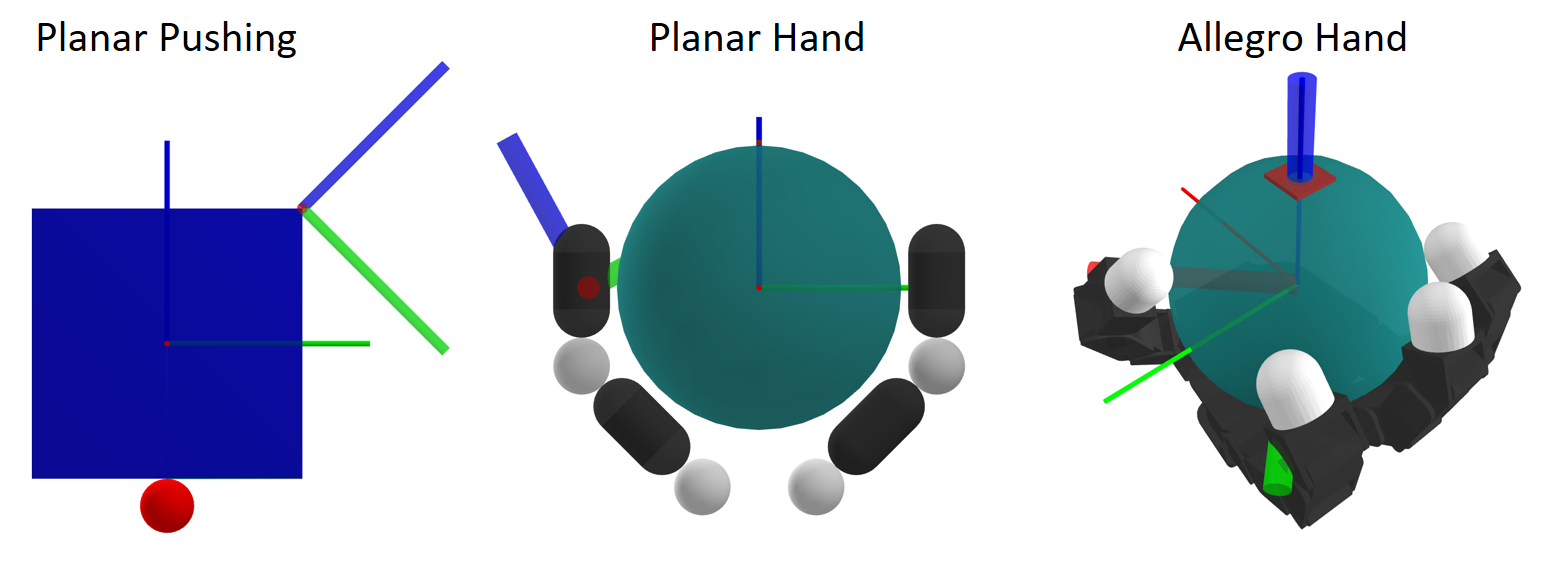
\includegraphics[width=0.80\textwidth]{figures/03_contact_rich_planning/trajopt_tasks.png}
	\label{fig:trajopttasks}
}\\
\subfloat[Final object configuration achieved by the best runs within each of the four methods. Pink shaded denotes the goal configuration for the first two examples, while the goal configuration in the last example is marked by the pink line protruding out of the object. Colors correspond to the plots in Fig. \ref{fig:trajoptperformance}.]{
    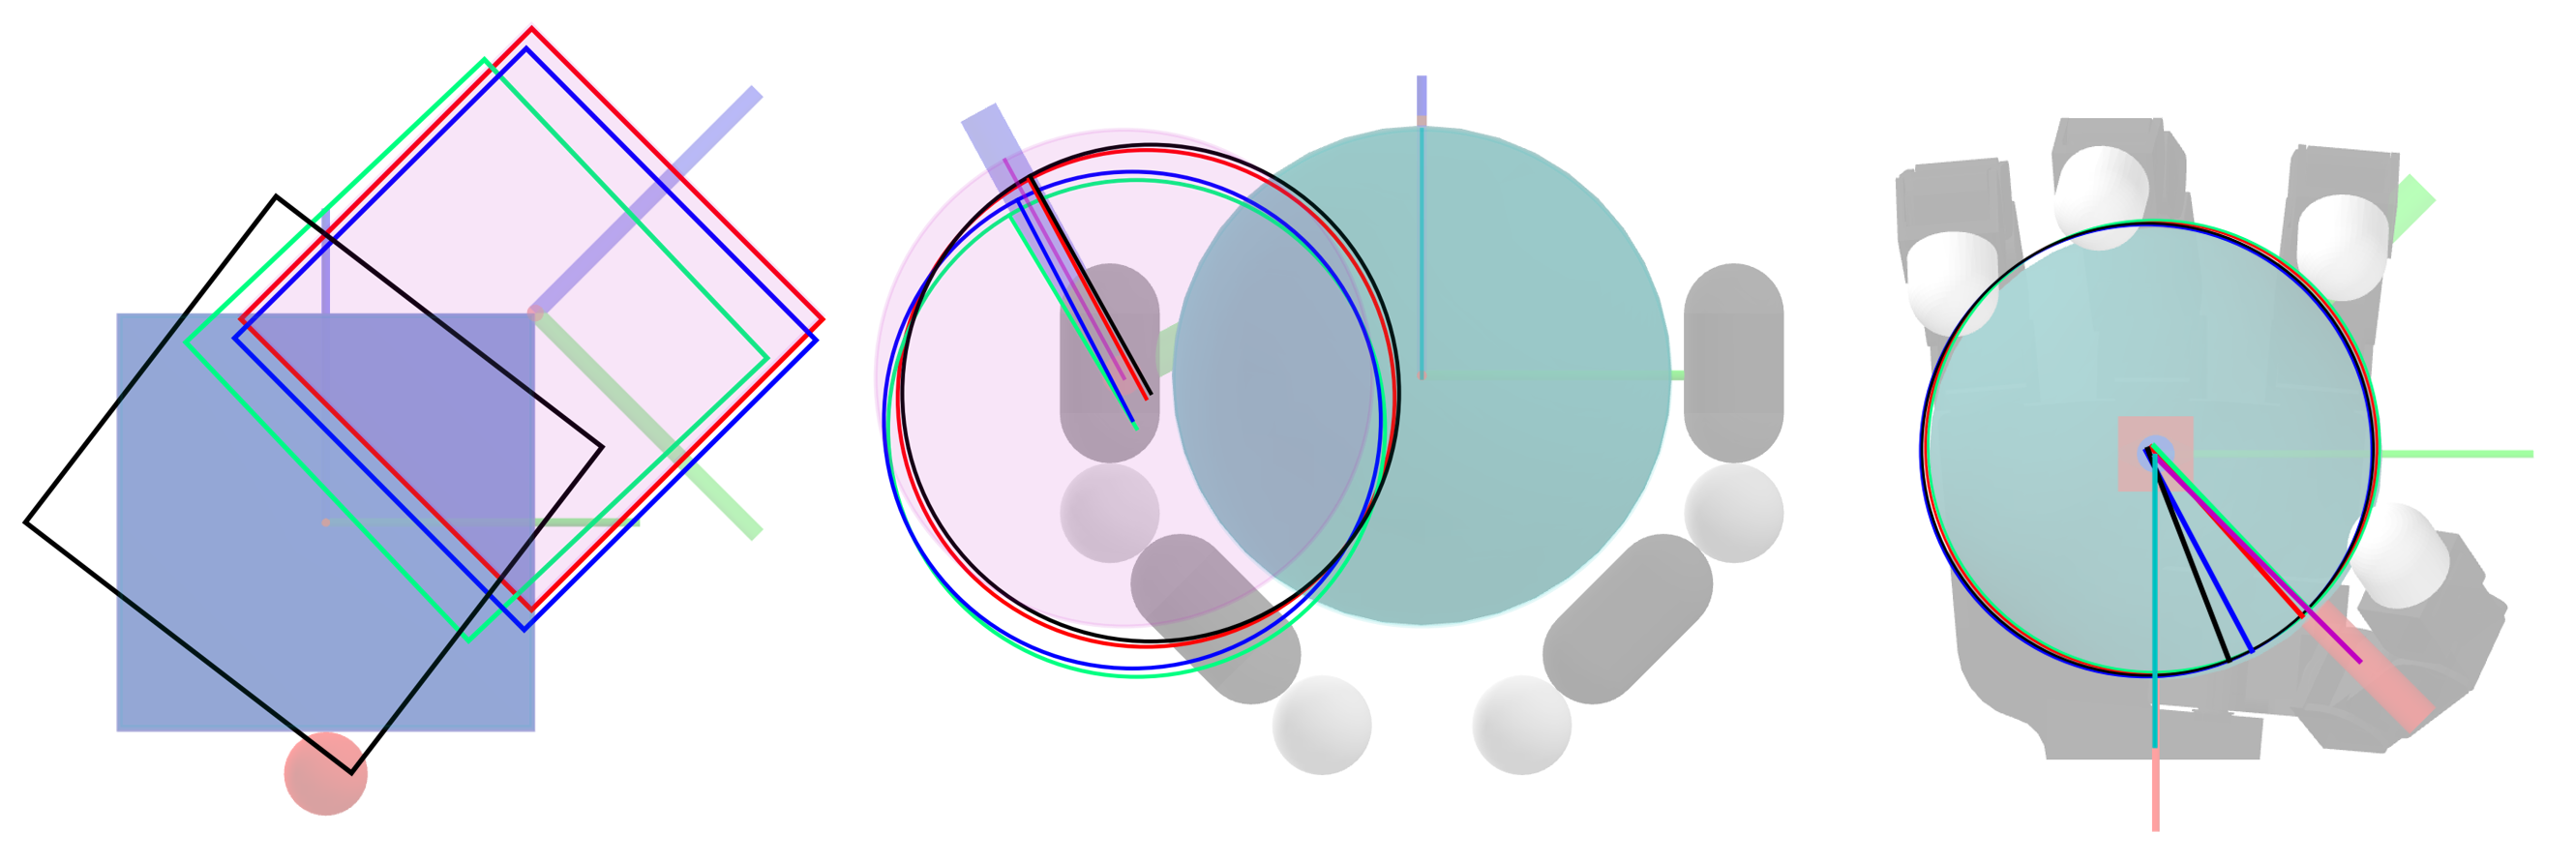
\includegraphics[width = 0.80\textwidth]{figures/03_contact_rich_planning/trajopt_results_vis.png}
    \label{fig:trajoptvis}
}
\caption{Tasks and results for the trajectory optimization case study.}
\label{fig:trajopt}
\end{figure}

\begin{table}[thpb] \label{tab:trajoptresults}
\centering
\begin{tabular}{|| c | r | r | r | r | r | r |} 
 \hline
 Problem & \multicolumn{2}{||c||}{PlanarPushing} & \multicolumn{2}{||c||}{PlanarHand} & \multicolumn{2}{||c||}{AllegroHand}  \\\hline
 Method & Cost & Time(s) & Cost & Time(s) & Cost & Time(s) \\ \hline\hline

    A.        & 11.74 & 2.17  & 26.55 &  5.20  & \bf{5.78} & 19.59  \\
    RF.       & \bf{11.73} & 4.64 & \bf{17.8}7 & 23.09 & 8.42 & 40.07 \\
    RZ.      & 12.86 & 4.61 & 18.29 & 11.93 & 28.21 & 34.05 \\
    E.            & 31.64 & 1.88 & 18.49 & 5.91 & 44.68 & 12.92 \\\hline
\end{tabular}
\caption{Minimum cost and running time achieved by different methods. All methods are ran for $10$ iterations across 5 trials. The methods names are abbreviations from the legend of Fig. \ref{fig:trajoptperformance}.}
\label{table:trajoptresults}
\vspace{-0.2cm}
\end{table}

%we note that we always initialize the system to be in a contacting configuration, as otherwise the gradient without smoothing is always zero in a non-contacting configuration. Consequently, algorithms that rely on exact linearization simply makes no progress. Though we initialize this way to give exact linearization an advantage, we note that the ability to converge from a non-contacting configuration is also a strength of using smooth surrogates.

\subsection{Results \& Discussion}
In Fig. \ref{fig:trajoptperformance}, we plot the performance of iMPC with a baseline that does not use smoothing, and the three different smoothing schemes in Sec. \ref{sec:smoothdynamics}, namely analytic, randomized first-order, and randomized zeroth-order. We also summarize the running time of each method, as well as the minimum cost achieved across the iterations, in Table \ref{table:trajoptresults}. Illustrations of the tasks and the results achieved by different methods are shown in Fig. \ref{fig:trajopt}. We interpret the results and discuss the relevant findings in this section. 
\subsubsection{Exact vs. Smoothing} For \code{PlanarPushing} and \code{AllegroRotation}, the various smoothing schemes achieve much lower costs than using exact gradients. However, for \code{PlanarHand}, using the exact linearization is performant as well. This difference may be explained by the observation that the planar hand example does not go through many mode changes, while the planar pusher and the allegro hand require several mode changes to converge to the locally optimal trajectory. 

\subsubsection{Analytic vs. Randomized Smoothing} Comparing the performance of the three smoothing schemes, the analytic and the first-order randomized smoothing perform similarly, while the zeroth-order version does not perform as well. We believe the cause lies in the high variance characteristic of the zeroth-order estimator in higher dimensions.


\subsubsection{Running (wall-clock) Time} While analytic smoothing only requires one evaluation of the smoothed dynamics \eqref{eq:q_dynamics_log} in order to compute $(\mathbf{A}_\rho,\mathbf{B}_\rho,c_\rho)$, randomized smoothing requires taking $N$ samples and averaging them, which costs $N$ times more compute-time. After parallelization, we expect randomized smoothing to be roughly $N/\xi$ times slower than analytic smoothing where $\xi$ is the number of threads. Indeed, with $N=100$ and $\xi=32$, our results show that randomized smoothing is 2 to 3 times slower than analytic smoothing.



\section{Local Mahalanobis Metric for RRT}
\label{sec:mahalanobis}
\noindent While trajectory optimization can find trajectories reaching goals that are close to the initial configuration, it is highly prone to local minima when the goal is further away (e.g. moving the box back in \code{PlanarPushing}, rotating the ball by 180 degrees in \code{PlanarHand}, \code{AllegroHand}). To solve these tasks, the planning algorithm needs to be more global. When faced with such problems, the RRT algorithm \cite{lavalle1998rapidly} has proven to be a classical and effective method for global planning. 

However, extending RRT to dynamical systems (i.e. kinodynamic RRT) has been difficult, as a distance metric between two states is hard to define. In \cite{shkolnik2009reachability}, it was argued that a good distance metric for RRT would need to explicitly consider dynamic reachability in order to efficiently grow the tree. The authors further proposed Reachability-Guided RRT (RG-RRT), which had system-specific reachability metrics that was shown to be effective for smooth systems. To alleviate the limitation of being system-specific, later works have considered building such metrics based on local characteristics of the dynamics such as local linearizations \cite{haddad2021anytime,wu2020r3t}.

However, when the dynamics involves contact, such local linearizations are no longer informative, and existing approaches often tackle dynamic reachability by explicitly considering contact modes \cite{chen2021trajectotree,cheng2021contact}. This has led to planners that scale poorly with the number of contacts. In contrast, we propose to handle the challenges brought about by contact with smoothing. We show that when combined with smoothing, the locally linear model can be used to construct an informative distance metric that is consistent with notions of reachability. 

\begin{figure*}
\centering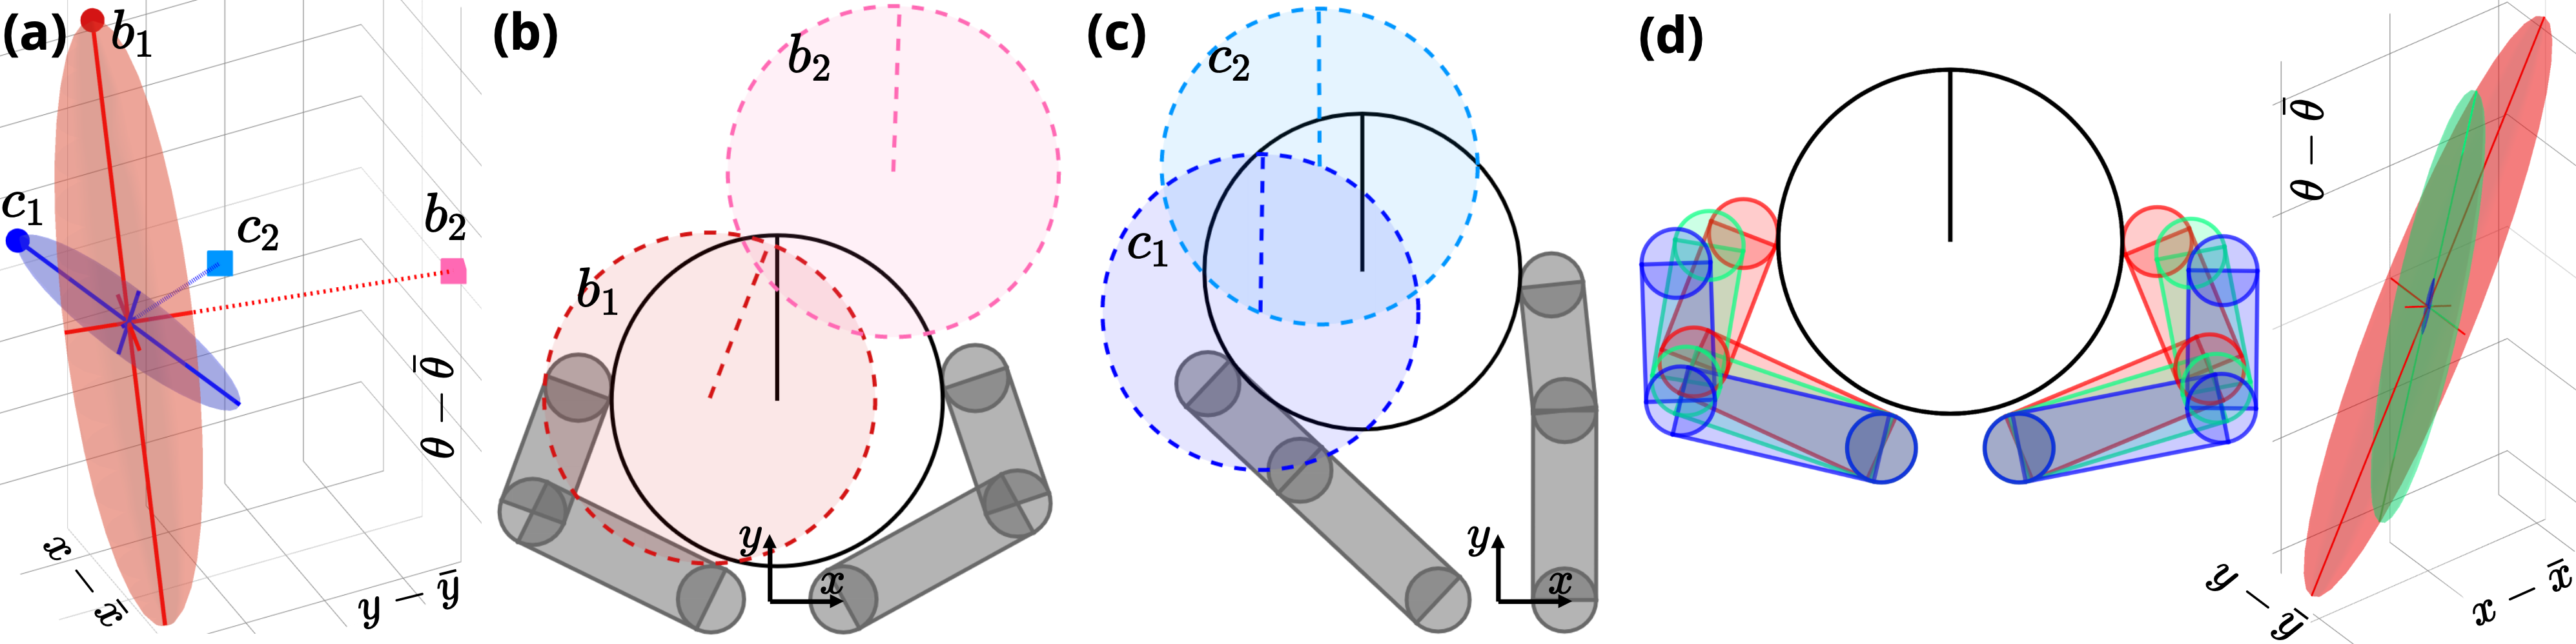
\includegraphics[width=1.0\textwidth]{figures/03_contact_rich_planning/reachability_planar_hand5.png}
\caption{(\textbf{a}) Two different sublevel sets $\mathcal{R}^\mathrm{u}_{\rho, \varepsilon, \gamma}$, represented as ellipsoids, shown in the space of $\qu$, with $\varepsilon = 1$, and $\gamma = 10^{-6}$. The ellipsoid centers are shifted to the origin for easy comparison. Red ellipsoid: $\mathcal{R}^\mathrm{u}_{\rho, \varepsilon, \gamma}$ for the system configuration in Fig. \ref{fig:reachability_planar_hand}b; blue ellipsoid: $\mathcal{R}^\mathrm{u}_{\rho, \varepsilon, \gamma}$ for the configuration in Fig. \ref{fig:reachability_planar_hand}c. Points $b_1$, $c_1$ are where ellipsoids' major axes intersect their boundaries. Points $b_2$, $c_2$ are points along the minor axes of the ellipsoids, and satisfy $\norm{b_1} = \norm{b_2}$ and $\norm{c_1} = \norm{c_2}$, where the norm is based on the standard Euclidean metric.
(\textbf{b}) The solid robots and objects represent the $\bar{q}$ at which the red $\mathcal{R}^\mathrm{u}_{\rho, \varepsilon, \gamma}$ in (a) is computed. The straight line on the puck indicates its orientation. The dashed dark red puck corresponds to the configuration $b_1$, and pink to $b_2$. Note that $b_1$ is easier to each than $b_2$.
(\textbf{c}) Similar to Fig. \ref{fig:reachability_planar_hand}b, the dashed dark blue puck correspond to $c_1$, and light blue to $c_2$. It is also easier to reach $c_1$ than $c_2$.
(\textbf{d}) The volume of $\mathcal{R}^\mathrm{u}_{\rho, \varepsilon, \gamma}$ shrinks as the fingers get further away from the puck. The ellipsoids on the right are color-coded to match the robot configurations on the left. Note that the blue ellipsoid is barely visible.}
\label{fig:reachability_planar_hand}

\end{figure*}

\subsection{The Local Mahalanobis Metric}

Consider the following problem: given the current configuration $\bar{q}$, and some queried configuration $q$, how can we formulate a distance metric $d(q;\bar{q})$ that is consistent with reachability characteristics of the system? We propose to utilize the locally linear model around the nominal configuration $\bar{q}$, that characterizes the local response of the next system configuration $q_+$ with respect to the movement of the actuated configurations $u$. This local model can be written as 
\begin{equation}
    q_+ = \mathbf{B}(\bar{q},\bar{q}^{\mathrm{a}})\underbrace{(u - \bar{q}^\mathrm{a})}_{\delta u} + c(\bar{q},\bar{q}^{\mathrm{a}})
\end{equation}
where the notation is consistent with the CQDC dynamics formulation in Sec.\ref{sec:convex_quasi_dynamic_contact_dynamics}; the input $u$ is the position command to the system), and $\mathbf{B},c$ are defined as \eqref{eq:linearization}. We note that the contribution of $\mathbf{A}$ term is zero since $\delta x = 0$.

Given such a local characterization, and a queried state $q$, we define the Mahalanobis metric as follows.
\begin{definition}
{\bf Local Mahalanobis Metric.}\normalfont \label{def:mahalanobis}
Given a nominal configuration $\bar{q}$, and queried configuration $q$, we define the Mahalanobis distance $d_\gamma$ of $q$ from $\bar{q}$ as follows:
\begin{equation}
\label{eq:metric}
\begin{aligned}
d_{\gamma}(q;\bar{q}) & \coloneqq \|q - \mu\|_{\mathbf{\Sigma}^{-1}_{\gamma}}=\textstyle\frac{1}{2}(q-\mu)^\intercal\mathbf{\Sigma}^{-1}_\gamma (q-\mu) \\
\mathbf{\Sigma}_{\gamma} & \coloneqq \mathbf{B}(\bar{q},\bar{q}^\mathrm{a})\mathbf{B}(\bar{q},\bar{q}^\mathrm{a})^\intercal + \gamma\mathbf{I}_n, \; \mu \coloneqq c(\bar{q},\bar{q}^\mathrm{a}).
\end{aligned}
\end{equation}
\end{definition}

The regularization $\gamma\mathbf{I}_n$ is added to ensure that $\mathbf{\Sigma}_{\gamma}$ is positive definite and the inverse $\mathbf{\Sigma}^{-1}_{\gamma}$ is well-defined. Note that the $\varepsilon$-sublevel set of this metric $d_\gamma(q;\bar{q})$, which we denote by $\mathcal{R}_{\varepsilon,\gamma}(\bar{q})$, describes an \emph{ellipsoid} that is centered at $\mu$ and has a shape matrix $\mathbf{\Sigma}^{-1}_\gamma$. We further motivate our construction of the metric by noting that this ellipsoid can be alternatively characterized (equivalent up to a regularization) by the following set, 
\begin{equation}
    \mathcal{R}_{\varepsilon}(\bar{q})\coloneqq \left\{\mathbf{B}(\bar{q},\bar{q}^{\mathrm{a}}) \delta u + c(\bar{q},\bar{q}^\mathrm{a})\; | \; \|\delta u\|\leq \varepsilon\right\}.
\end{equation}

This equivalence relation is exact when $\mathbf{B}$ has full row rank (i.e. the system is one-step controllable) and $\gamma=0$. On the other hand, if $\mathbf{B}$ loses rank, one of the principle axis of $\mathcal{R}_{\varepsilon}$ has a length of zero and the set becomes degenerate.

Finally, note that when $q-\mu \notin \mathbf{Range}(\mathbf{B})$, i.e. there is no actuation $u$ that can take the state $\bar{q}$ to the queried state $q$, the distance $ d_{\gamma}(q;\bar{q})$ is a large number dominated by the inverse of the regularization term $\gamma^{-1}$, which is consistent with the intuition that states that are harder to reach are further away.

\subsection{Metric on Smoothed Dynamics and Unactuated Objects}
\label{sec:smooth_metric}
As explained in the previous sections, the local model constructed using $\mathbf{B}$ may not be a very informative one for non-smooth systems with contact. In light of the various smoothing schemes introduced in Sec.\ref{sec:smoothdynamics} to alleviate this issue, we propose a metric by utilizing the linearization of the smooth surrogate $(\mathbf{B}_\rho,c_\rho)$, as opposed to those of the original contact dynamics, $(\mathbf{B},c)$. 

Furthermore, for systems where robots interact with unactuated objects through contact, we focus on the reachability of the objects, as the robots are actuated and can easily move to a desired configuration without contact. We combine smoothing and the object-centric reachability in the following variant of the Mahalanobis metric $d^\mathrm{u}_{\rho,\gamma}$, 
\begin{equation}
\label{eq:unactuated_mahalanobis_metric}
\begin{aligned}
d_{\rho,\gamma}^\mathrm{u}(q;\bar{q}) & \coloneqq \|q^\mathrm{u} - \mu^\mathrm{u}_\rho\|_{\mathbf{\Sigma}^{\mathrm{u}^{-1}}_{\rho,\gamma}}, \\
\mathbf{\Sigma}_{\rho,\gamma}^\mathrm{u} & \coloneqq \mathbf{B}^\mathrm{u}_\rho(\bar{q},\bar{q}^\mathrm{a})\mathbf{B}^\mathrm{u}_\rho(\bar{q},\bar{q}^\mathrm{a})^\intercal + \gamma\mathbf{I}_{n_\mathrm{u}},\\ 
\mu_\rho^\mathrm{u} & \coloneqq c_\rho^\mathrm{u}(\bar{q},\bar{q}^\mathrm{a}).
\end{aligned}
\end{equation}
where $\mathbf{B}^\mathrm{u}_\rho$ is formed by the rows of $\mathbf{B}_\rho$ corresponding to the unactuated DOFs, and $c_\rho^\mathrm{u}$ is defined similarly. Finally, we define $\mathcal{R}_{\rho,\varepsilon,\gamma}^\mathrm{u}(\bar{q})$ as the $\varepsilon$-sublevel set of $d^\mathrm{u}_{\rho,\gamma}(q;\bar{q})$. 

In the rest of this section, we give several examples that provide intuition into the local Mahalanobis metric $d^\mathrm{u}_{\rho,\gamma}$ and its sublevel set $\mathcal{R}^\mathrm{u}_{\rho,\varepsilon,\gamma}$. 

\begin{example} \normalfont \textbf{(Understanding $\B$ for Planar Systems)}
As shown in Sec. \ref{sec:quasi_static:artifacts}, \ref{sec:trajopt_setup:systems}), the CQDC dynamics \eqref{eq:q_dynamic_socp} simplifies to a QP \eqref{eq:q_dynamics_planar_qp} for planar systems. For reference, the QP \eqref{eq:q_dynamics_planar_qp} is reproduced below:
\begin{subequations}
\label{eq:q_dynamics_planar_qp_copy}
\begin{align}
\underset{\dq}{\minimize} \; &\frac{1}{2} \dq^\intercal \mathbf{Q} \dq + b^\intercal \dq, \; \text{subject to} \\
&(\Jn[i] + \mu_i \Jt[i]) \dq + \phi_i \geq 0, \; i \in \{1\dots\nC\}, \label{eq:q_dynamics_planar_qp_copy:constraint1}\\
&(\Jn[i] - \mu_i \Jt[i]) \dq + \phi_i \geq 0, \; i \in \{1\dots\nC\}. \label{eq:q_dynamics_planar_qp_copy:constraint2}
\end{align}
\end{subequations}
Recall that the contact Jacobian $\Jt[i]$ has only one row instead of two. We define $\J \in \R[(2\nC) \times n_q]$ by stacking the $\Jn[i] + \mu_i \Jt[i]$ and $\Jn[i] - \mu_i \Jt[i]$ from \eqref{eq:q_dynamics_planar_qp_copy:constraint1} and \eqref{eq:q_dynamics_planar_qp_copy:constraint2} into a single matrix, and partition $\J$ into $\Ju$ and $\Ja$ in a similar way as in \eqref{eq:contact_jacobian_i}.

More structure behind the $\mathbf{B}$ matrix (as defined in \eqref{eq:q_dynamics_AB}) can be revealed with a bit of linear algebra. We can work out by hand the application of the implicit function theorem to the KKT conditions of \eqref{eq:q_dynamics_planar_qp}, and the chain rule in \eqref{eq:DdqDu}, to obtain an explicit expression for $\B$:
\begin{subequations}
\label{eq:planar_B_structure}
\begin{align}
\mathbf{B} &=
\begin{bmatrix}
\Ba \\ 
\Bu
\end{bmatrix}
=
\begin{bmatrix}
\mathbf{I} - (h^2\Ka)^{-1} (\JaActive)^\intercal \mathbf{P} \JaActive \\
\Mu^{-1} (\JuActive)^\intercal \mathbf{P} \JaActive
\end{bmatrix}, \; \text{with}\\
\mathbf{P} &= \left[\JuActive \Mu^{-1} (\JuActive)^\intercal + \JaActive (h^2 \Ka)^{-1} (\JaActive)^{\intercal} \right]^{-1}.
\end{align}
\end{subequations}
where we assume $\JuActive$ and $\JaActive$ have full row rank. The tilde over a Jacobian indicates the sub-matrix formed by rows of the original matrix corresponding to the active constraints, i.e. contacts with non-zero contact forces.

%The robot actuation matrix, $\Ba$, is the difference between identity and a term that decreases as $\Ka$ grows, which is intuitively saying that a stiff robot usually goes to where it is asked to go. As for $\Bu$, it is noteworthy that the possible object motions in a specific contact mode live in the range of $(\JuActive)^\intercal$, the transpose of the active contact Jacobian. 

The structure in $\Bu$ explains why $\Bu_\rho$ is a good measure of the object's reachability when there is contact.
We can interpret $\mathbf{Range}(\JuActive^\intercal)$ as achievable object motions under the specific subset of active contacts.
By averaging $\Bu$ computed from different contacts which can be activated from the nominal $(\bar{q}, \bar{u})$, $\Bu_\rho$ summarizes possible object motions due to contact, in the form of $\mathbf{Range}(\JuActive^\intercal)$ weighted by $\Mu$ and $\mathbf{P}$. 

Furthermore, for a configuration with no active contacts, \eqref{eq:planar_B_structure} implies that $\Ba = \I$ and $\Bu = \mathbf{0}$, as both $\JaActive$ and $\JuActive$ are empty matrices in the absence of active contacts. This has the intuitive interpretation that under a $u$ that does not lead to contacts, the robot will move to where it is commanded to, and the object will remain still.

As $\mathbf{B}_\rho^\mathrm{u}$ is the expected value of $\mathbf{B}^\mathrm{u}$, it follows naturally from the above observation that the local distance metric $d_{\rho, \gamma}^\mathrm{u}$ tends to be dominated by the regularization $\gamma \mathbf{I}_{n_\mathrm{u}}$ for a nominal configuration $\bar{q}$ where robots and objects are far from making contact. In such cases, the probability that an action $u$ sampled from a distribution $\rho$ centered at $\bar{q}^\mathrm{a}$ leads to active contacts is low. As a result, in the Monte-Carlo estimation of $\mathbf{B}_\rho^\mathrm{u}$, such samples simply introduce $\mathbf{0}$ into the average, dragging the distance metric $d^\mathrm{u}_{\rho,\gamma}$ towards being dominated by the regularization.
\end{example}



\begin{example} \normalfont \textbf{(Metric on Planar Hand)}
\label{ex:planarhandreachableset}
We illustrate how the Mahalanobis metric can guide planning using the \code{PlanarHand} system first introduced in Sec. \ref{sec:trajopt_setup}.
As shown in Fig. \ref{fig:reachability_planar_hand}, the system lives in the $xy$ plane, with gravity pointing into the paper along the negative $z$ direction. The system consists of two actuated 2-link robotic fingers and an unactuated puck which is free to translate and rotate. Each finger can interact with the ball through frictional contacts along both links.

For a given $\qu$, the difficulty of reaching $\qu$ from $(\bar{q}, \bar{u})$ can be measured by the local Mahalanobis metric $d^\mathrm{u}_{\rho, \gamma}$, whose $1$-sublevel sets are shown in Fig. \ref{fig:reachability_planar_hand}a as ellipsoids. Although object configurations $b_1$ and $b_2$ are equidistant to the origin under the globally-uniform Euclidean metric, $b_1$ is considered much closer than $b_2$ under the local Mahalanobis metric (red ellipsoid). Indeed, in Fig. \ref{fig:reachability_planar_hand}b, reaching $b_1$ from the current puck configuration seems easier than reaching $b_2$. A similar observation can be made for the configuration in Fig. \ref{fig:reachability_planar_hand}c.

In addition, the local Mahalanobis metric also varies greatly from one configuration another, as evidenced by the difference between the blue and red ellipsoids in Fig. \ref{fig:reachability_planar_hand}a. This implies that a globally-uniform metric is rarely a good measure of reachability characteristics.

Lastly, the ellipsoid that corresponds to the $1$-sublevel set shrinks as the nominal state gets further away from the contact manifold, as shown in Fig. \ref{fig:reachability_planar_hand}d. This signifies that the configurations where the object is less accessible by the robot are naturally considered ``further away'' and can thus be avoided by the planner.
\end{example}


\section{RRT through Contact \label{sec:rrt_for_contact}}
\noindent We are now ready to present our smoothing-based enhancements to the vanilla RRT algorithm, which we reproduce in Alg. \ref{alg:rrt} to establish notations for our discussion. Our method enhances RRT by incorporating
(\textbf{i}) a reachability-aware $\Nearest$ operation based on the smoothed Mahalanobis metric on the unactuated objects $d_{\rho,\gamma}^\mathrm{u}$,
% a $\mathtt{Nearest}$ operation based on the object Mahalanobis reachability metric $d_{\rho,\gamma}^\mathrm{u}$ of individual nodes constructed on the smoothed dynamnics;
(\textbf{ii}) a fast $\Extend$ operation based on the projection of the subgoal to the range of $\mathbf{B}_\rho$; and
(\textbf{iii}) a contact sampling procedure which improves the reachability of nodes added to the tree.

We denote the RRT tree as $\mathcal{T}=(\mathcal{V},\mathcal{E})$ with vertex set $\mathcal{V}$ and edge set $\mathcal{E}$. Each node $q \in \mathcal{V}$ is simply a point in the configuration space of the system. 


\begin{algorithm}[t]
\caption{\textbf{RRT}}\label{alg:rrt}
\textbf{Input:} $q_{\mathrm{init}}, q_{\mathrm{goal}}, K$\;
\textbf{Output:} $\mathcal{T}$\;
$\mathcal{T} = \{q_{\mathrm{init}}\}$\;
\For {$k = 1, \dots, K$}{
    % \While{$\mathtt{IsInvalid}(v_{\mathrm{nearest}})$}
    $q_{\mathrm{subgoal}} = \mathtt{SampleSubgoal(p)}$\;
    $q_{\mathrm{nearest}} = \mathtt{Nearest}(q_{\mathrm{subgoal}})$\; \label{alg:rrt:nearest}
    % \EndWhile
    $q_{\mathrm{new}} = \mathtt{Extend}(q_{\mathrm{nearest}}, q_{\mathrm{subgoal}})$\;  \label{alg:rrt:extend}
    % \State $\mathcal{T}.\mathtt{Rewire(v_{\mathrm{new}})}$
    $\mathtt{AddNode}(q_{\mathrm{new}})$ \label{alg:rrt:add_node}\;
    \If{\texttt{GoalReached}}{$\textbf{break}$\;}
}
\end{algorithm}


\subsection{Nearest Node using Local Mahalanobis Metric}
As illustrated in Sec.\ref{sec:mahalanobis}, in particular by Example \ref{ex:planarhandreachableset}, a globally-uniform metric used by the vanilla RRT is usually a poor measure of reachability. Given a subgoal $q_{\mathrm{subgoal}}$, if the nearest node $q_{\mathrm{nearest}}$ is chosen under a globally-uniform metric, reaching $q_{\mathrm{subgoal}}$ from $q_{\mathrm{nearest}}$ may require large $u$ or even be dynamically infeasible. This will compromise RRT's ability to explore the configuration space, as trying to $\mathtt{Extend}$ towards a hard-to-reach $q_{\mathrm{subgoal}}$ typically returns a child node that is close to the parent node $q_{\mathrm{nearest}}$. In order to retain RRT's ability to efficiently explore under dynamics constraints, we use the smoothed Mahalanobis metric \eqref{eq:unactuated_mahalanobis_metric} instead of the usual Euclidean metric in the $\mathtt{Nearest}$ step:
\begin{equation}
q_{\mathrm{nearest}} = \text{argmin}_{q \in \mathcal{V}}\; d^{\mathrm{u}}_{\rho,\gamma}(q_{\mathrm{subgoal}}; q).
\end{equation}

\subsection{Dynamically Consistent Extension}
After choosing $q_{\mathrm{nearest}}$ from the tree $\mathcal{T}$, we need an action or a sequence of actions that moves the system from $q_{\mathrm{nearest}}$ to $q_{\mathrm{subgoal}}$ subject to the dynamics constraint. One feasible strategy to connect $q_{\mathrm{nearest}}$ to $q_{\mathrm{subgoal}}$ is to solve for an input sequence $\{u_t\}_{t=0}^{T-1}$ using a trajectory optimization algorithm such as Alg. \ref{alg:impc} \cite{karaman2010optimal}. However, the high computational cost of trajectory optimization motivates us to seek a simpler solution.

Fortunately, as a result of the farsightedness of quasi-static models, even an input sequence with $T = 1$ (i.e. a single time step) can steer the system fairly far away from $q_{\mathrm{nearest}}$. Although trajectory optimization with $T > 1$ can explore a larger region around $q_{\mathrm{nearest}}$, we find in practice that a single time step is sufficient for $\Extend$ to effectively grow the RRT tree $\mathcal{T}$.

We present the modified $\Extend$ that uses a single time step in Alg. \ref{alg:extend}. The input $u$ is computed by projecting $(q^\mathrm{u}_{\mathrm{subgoal}} - \mu_\rho^\mathrm{u})$ to $\mathbf{Range}(\Bu_\rho)$ using least squares (Line \ref{alg:extend:lstsq}), which is significantly cheaper than solving trajectory optimization. Afterwards, we normalize the input and multiply it by some stepsize $\varepsilon$. The scaled input is then passed to the forward dynamics to obtain a new node. Crucially, we use the actual dynamics $f$ as opposed to the smooth surrogate dynamics $f_\rho$ (Line \ref{alg:extend:rollout}). This ensures that while the search for the next action relies on the smoothed model, the actual path is dynamically consistent under the original non-smooth contact dynamics (i.e. CQDC). 

\begin{algorithm}
\caption{$\mathtt{Extend}$}\label{alg:extend}
\textbf{Input:} $q_{\mathrm{nearest}}, q_{\mathrm{subgoal}}$\;  \textbf{Output:} $q_{\mathrm{new}}$\;
$\delta u^\star = \mathrm{argmin}_{\delta u} \|\Bu_\rho \delta u + c_\rho^\mathrm{u} - q_{\mathrm{subgoal}}^\mathrm{u} \|$ \label{alg:extend:lstsq} \;
% $\varepsilon = \min(\varepsilon_\mathrm{max}, \norm{\delta u^\star})$ \label{alg:extend:cap}\;
\algorithmicreturn  $\; f(q_{\mathrm{nearest}}, q_{\mathrm{nearest}}^\mathrm{a} + \varepsilon \cdot \delta u^\star / \|\delta u^\star\|)$ \label{alg:extend:rollout}\;
\end{algorithm}


\subsection{Contact Sampling}\label{sec:contactsampling}
A node $q$ where robots and objects are far from making contacts hinders the growth of the RRT tree for two reasons. First, such nodes are considered far away under the local Mahalanobis metric from most sampled $q_\mathrm{subgoal}$, as the sublevel sets of their Mahalanobis distance metric have small volume (e.g. Fig. \ref{fig:reachability_planar_hand}d). As a result, adding such nodes to the tree simply increases ``deadweight'' without improving coverage of the state space. Moreover, when such a node is chosen by $\Nearest$, the $\Extend$ operation that follows often results in another non-contact configuration.

To reduce the number of such nodes in $\mathcal{T}$ and improve exploration during tree growth, the $\Extend$ operation is replaced, with some probability, by a new operation called $\ContactSample$. $\ContactSample$ takes $q_\mathrm{nearest}$ as input, and creates another node with a better local metric by fixing $q_\mathrm{nearest}^\mathrm{u}$ and finding an informative $q_\mathrm{nearest}^\mathrm{a}$ that makes contact with the object. 

The $\ContactSample$ operation is essential for adequate exploration of the robot's state space, and needs to be designed differently for different robots. 
As an example, we briefly describe how $\ContactSample$ is implemented for the three robots shown in Fig. \ref{fig:rrt_tasks}, which are used in our experiments in Sec. \ref{sec:rrt_results}. 
\begin{itemize}
\item \code{PlanarPushing}. The robot (the red sphere) is placed at a random point sampled on the perimeter of the box. 
\item \code{PlanarHand}. The robot consists of two fingers that can be treated as two-link robot arms. There are two different ways for the robot to contact the sphere: 
(\textbf{i}) \emph{enveloping} grasps, where for each finger, we start with the finger straight and horizontal, and then rotate each joint towards the ball until all links are touching the ball; 
(\textbf{ii}) \emph{pinch} grasps, where for each finger, we sample a point on the sphere, and solve inverse kinematics to find a finger configuration that touches the ball at the fingertip. 
\item \code{AllegroHand} (in all 4 systems with the hand). We start with the hand open and near the object (for \code{AllegroDoor} the object is the door knob). We then close the hand along a randomly picked direction in the robot's joint space until the object is ``grasped''.  The direction is generated by a weighted average of several EigenGrasps directions \cite{eigengrasp}, where the weights are sampled randomly. 
\end{itemize}  

Contact sampling introduces non-physical behavior where the robot teleports from one configuration to another. This is not a problem when the object can sustain static equilibrium without the actuated DOFs that need to teleport. For instance, in \code{AllegroHand}, when the ball is supported by the palm, the fingers are free to move around the ball to regrasp. In contrast, if \code{AllegroHand} were facing downwards, the ball would fall under gravity if it were not secured by some of the fingers. Although this is a limitation of our current contact sampling implementation, we believe this can be resolved by a more sophisticated contact sampler which moves some of the actuated DOFs while keeping the object in static equilibrium with the rest. 

\subsection{Effectiveness of Proposed Enhancements \label{sec:rrt_contact_effectiveness}}

\begin{figure*}
\centering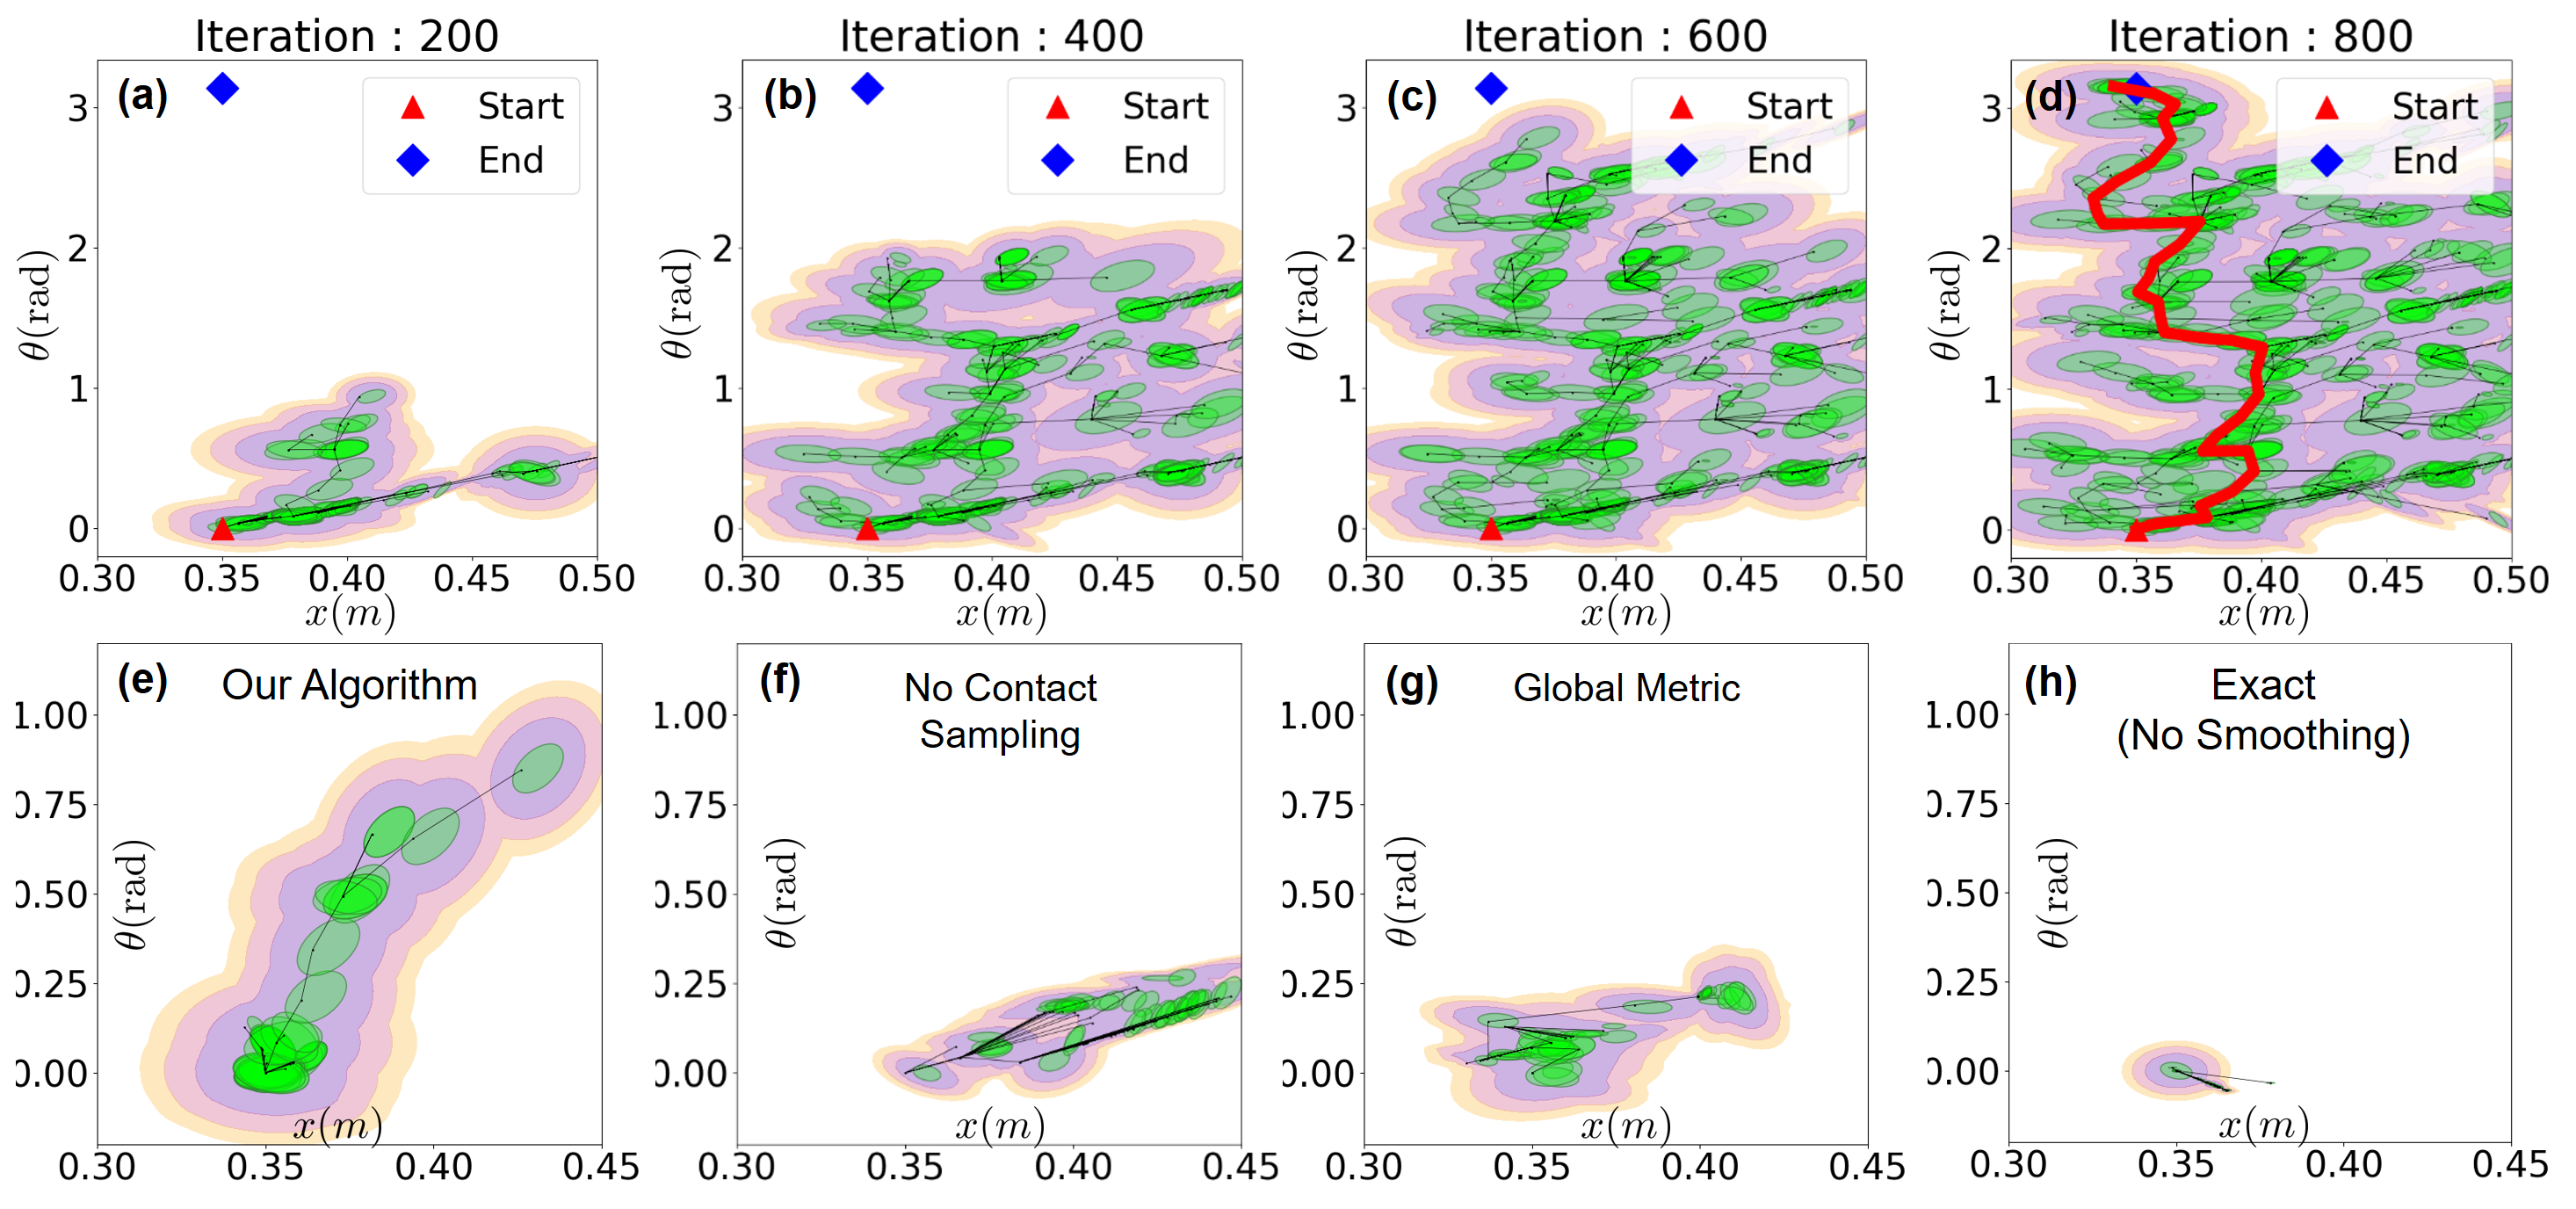
\includegraphics[width = 1.0\textwidth]{figures/03_contact_rich_planning/iteration_plot_combined_horizontal.png}
\caption{\textbf{(a-d)} RRT trees, shown in the space of $\qu$, at different iterations of a complete run of the enhanced RRT for the \code{PlanarHandFixedY} system. The contours are the sub-level sets of the local Mahalanobis metric of the nodes. The path from start ($q_\mathrm{init}$) to goal ($q_\mathrm{goal}$) is highlighted in red in the final tree of \textbf{(d)}. \textbf{(e-h)} Visualization of RRT trees with the same number of nodes (50) but grown with different methods. (\textbf{e}) Tree grown with our algorithm; (\textbf{f}) without contact sampling; (\textbf{g}) using a globally uniform weighted Euclidean metric; (\textbf{h}) using exact gradients without smoothing. Note that our method achieves the best coverage of the space of $\qu$.}
\label{fig:degenerate}
\end{figure*}

We introduce a new system with a 2-dimensional object configuration space to illustrate the effectiveness of the proposed RRT enhancements:
\begin{itemize}
\item {\bf Planar Hand with fixed $y$, (2,4,13)}. A simplified version of the \code{PlanarHand} system in Sec. \ref{sec:trajopt_setup}. We fix the $y$-coordinate of the object, so that $\qu = (x, \theta)\in \R[2]$ can be easily plotted on paper. 
\end{itemize}

As shown in Fig. \ref{fig:degenerate}e, the vanilla RRT enhanced with the proposed $\Nearest$, $\Extend$ and $\ContactSample$ achieves good coverage of the space of $\qu$, which is crucial for RRT to adequately explore the configuration space and find a path to $q_\mathrm{goal}$. In contrast, tree growth is stuck around the root without contact sampling (Fig. \ref{fig:degenerate}f) or the local metric (Fig. \ref{fig:degenerate}g).

We also illustrate how the tree grows throughout a complete run of the enhanced RRT in Fig. \ref{fig:degenerate}a-d. Even with the proposed enhancements, tree growth can get stuck at times. This is characterized by a specific type of subgraph of the tree which we call a ``broom''. A broom consists of one parent node with many child nodes, and is formed by repeated unsuccessful attempts to grow towards different subgoals from the same parent node. The occasional appearance of brooms is a sign that the proposed enhancements are not perfect. Nevertheless, the enhanced RRT is able to quickly branch out into empty part of the configuration space, and sufficiently cover the space as the tree grows. 

\subsection{Final Path Refinement}

The final path returned by the RRT algorithm is visually plausible, yet suffers from two minor drawbacks: (\textbf{i}) RRT tends to produce randomized paths that can be shortened, and (\textbf{ii}) the big step size used in the $\Extend$ operation creates some non-physical artifacts due to Anitescu’s convex relaxation of the Coulomb friction model (Sec.\ref{sec:convex_quasi_dynamic_contact_dynamics}). 

To mitigate these issues, we refine the RRT plan using trajectory optimization \cite{lgp,terry} and short-cutting \cite{shortcutting}. 
We first divide the RRT path into different segments punctuated by $\ContactSample$ operations. We call these segments contact-rich as they involve conact-based interactions between the object and the robot. 
For each contact-rich segment, we run trajectory opimization (Alg.\ref{alg:impc}) with a smaller time step $h$, using the RRT path segment as the initial guess. This not only smooths the final path, but also ensures that each trajectory segment is more physically realistic.
Then, we shortcut the sequence of trajectories by (\textbf{i}) removing consecutive $\ContactSample$ steps, and (\textbf{ii}) truncating each segment if there is no movement in $\qu$. 
Finally, we connect adjacent contact-rich segments with a collision-free robot trajectory created by a collision-free RRT. We assume that the object configuration remains unchanged during the collision-free segment.

We find that combining these two strategies is effective in creating shorter and more physically realistic trajectories. 

\begin{figure*}
\centering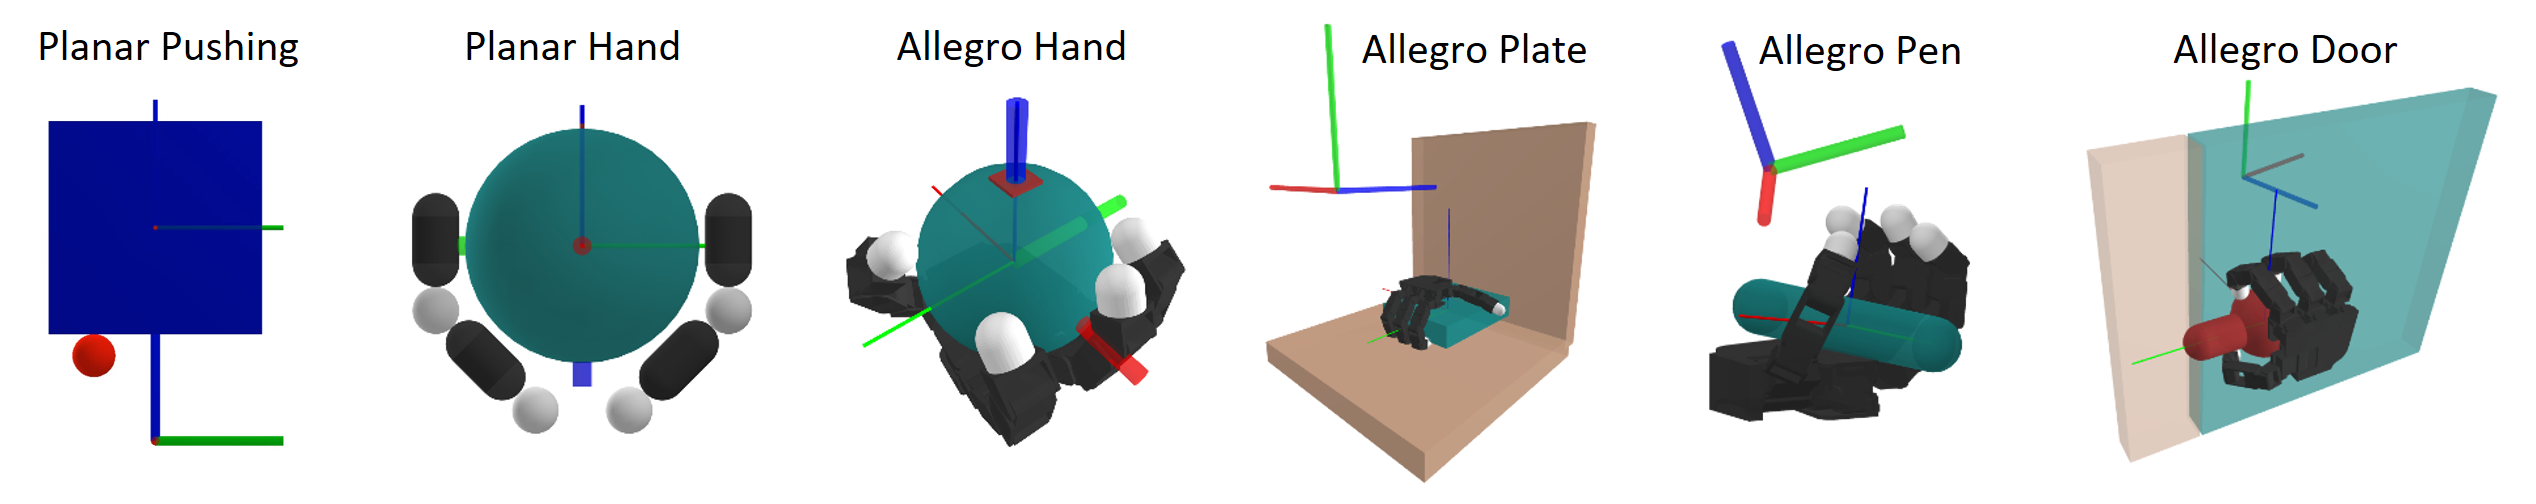
\includegraphics[width = 1.0\linewidth]{figures/03_contact_rich_planning/rrt_systems_pagewide.png}
\caption{Tasks for RRT. Similar to Fig. \ref{fig:trajoptvis}, the thicker frame denotes the goal, and the thinner frame the initial configuration of the object.}
\label{fig:rrt_tasks}
\end{figure*}



\section{Results \& Discussion \label{sec:rrt_results}}
\noindent In this section, we apply our algorithm on difficult 3D contact-rich manipulation problems previously only tackled by heavy offline approaches in RL \cite{rajeswaran2018learning, chen2022system}, and illustrate that we can generate plans on the order of a minute of online compute time, all on the CPU, which shows the efficacy of our method.
The experiments in this section are designed to validate the following four hypotheses.
\begin{enumerate}
\item Using the smooth surrogate greatly improves the performance over using the exact dynamics for linearization.
\item The equivalence of smoothing schemes establishes that analytic and randomized smoothing will have similar levels of performance empirically, with analytic smoothing showing superior computation time.
\item Using the Mahalanobis distance metric improves performance over a globally uniform distance metric.
\item Contact sampling greatly aids sample efficiency of the algorithm.
\end{enumerate}

\subsection{Experiment Setup \label{sec:rrt_experiment_setup}} 
To test the efficacy of our algorithm and the above stated hypotheses, we run our algorithm to reach more challenging goals than the trajectory optimization examples in Sec. \ref{sec:trajopt_setup:systems}, as well as on 3 more contact-rich tasks on 3 new systems defined below.
\begin{enumerate}
    \item {\bf Pen Placement (6,19,24)}. The robot hand needs to both translate and rotate the pen \cite{rajeswaran2018learning} to the desired configuration.
    \item {\bf Plate Pickup (6,19,42)}. The robot has to exploit the external contact between the plate and the wall \cite{cheng2021contact}, showing extrinsic dexterity \cite{extrinsic}.
    \item {\bf Door Opening (2,19,22)} \cite{rajeswaran2018learning} involves reasoning about a constrained system, where the handle must be rotated first before the door can be pushed open.
\end{enumerate}
The definition of the number tuples is identical to Sec.\ref{sec:trajopt_setup:systems}.

The contact-rich planning tasks are illustrated in Fig. \ref{fig:rrt_tasks}.
We design the tasks so that solving any of them with a single run of trajectory optimization is expected to fail due to their difficulty and the resulting non-convexity of the problem. 


To compare our algorithm with different baselines, we rate the quality of planners using two metrics:
\begin{enumerate}
    \item {\bf Iteration vs. Minimum distance to goal}.  we measure the distance between the goal and the tree, defined by $\min_{q\in\mathcal{V}} \|q^\mathrm{u} - q_\textrm{goal}^\mathrm{u}\|$ for every iteration. A successful planning algorithm would eventually reach the vicinity of the goal asymptotically, driving this metric to zero. 
    \item {\bf Iteration vs. Packing Ratio}. To characterize the \emph{exploration} performance of RRT, we do a Monte-Carlo estimation of the \emph{packing ratio}, which is defined as the volume of the space occupied by the reachability ellipses, divided by the total volume of some workspace limit for the unactuated objects. The workspace limit is the set from which subgoals are sampled when running RRT. More formally, we define the numerator as
    \begin{equation}
        V_{\mathrm{reachable}} = \textbf{vol}\big(\{q^\mathrm{u} | \min_{\bar{q}\in\mathcal{V}} d^\mathrm{u}_{\rho,\gamma}(q; \bar{q}) \leq \eta\}\big)
    \end{equation}
    where $\eta$ is some threshold on the distance metric. The Monte-Carlo estimate of $V_{\mathrm{reachable}}/V_{\mathrm{workspace}}$ can be computed by drawing $N$ samples within the workspace and counting how many of them belong to $V_{\mathrm{reachable}}$. A good planner should asymptotically reach a ratio of $1$ if the system can reach all points in the workspace.
\end{enumerate}

\begin{figure}
\centering
\subfloat[Planar Pushing.]{
	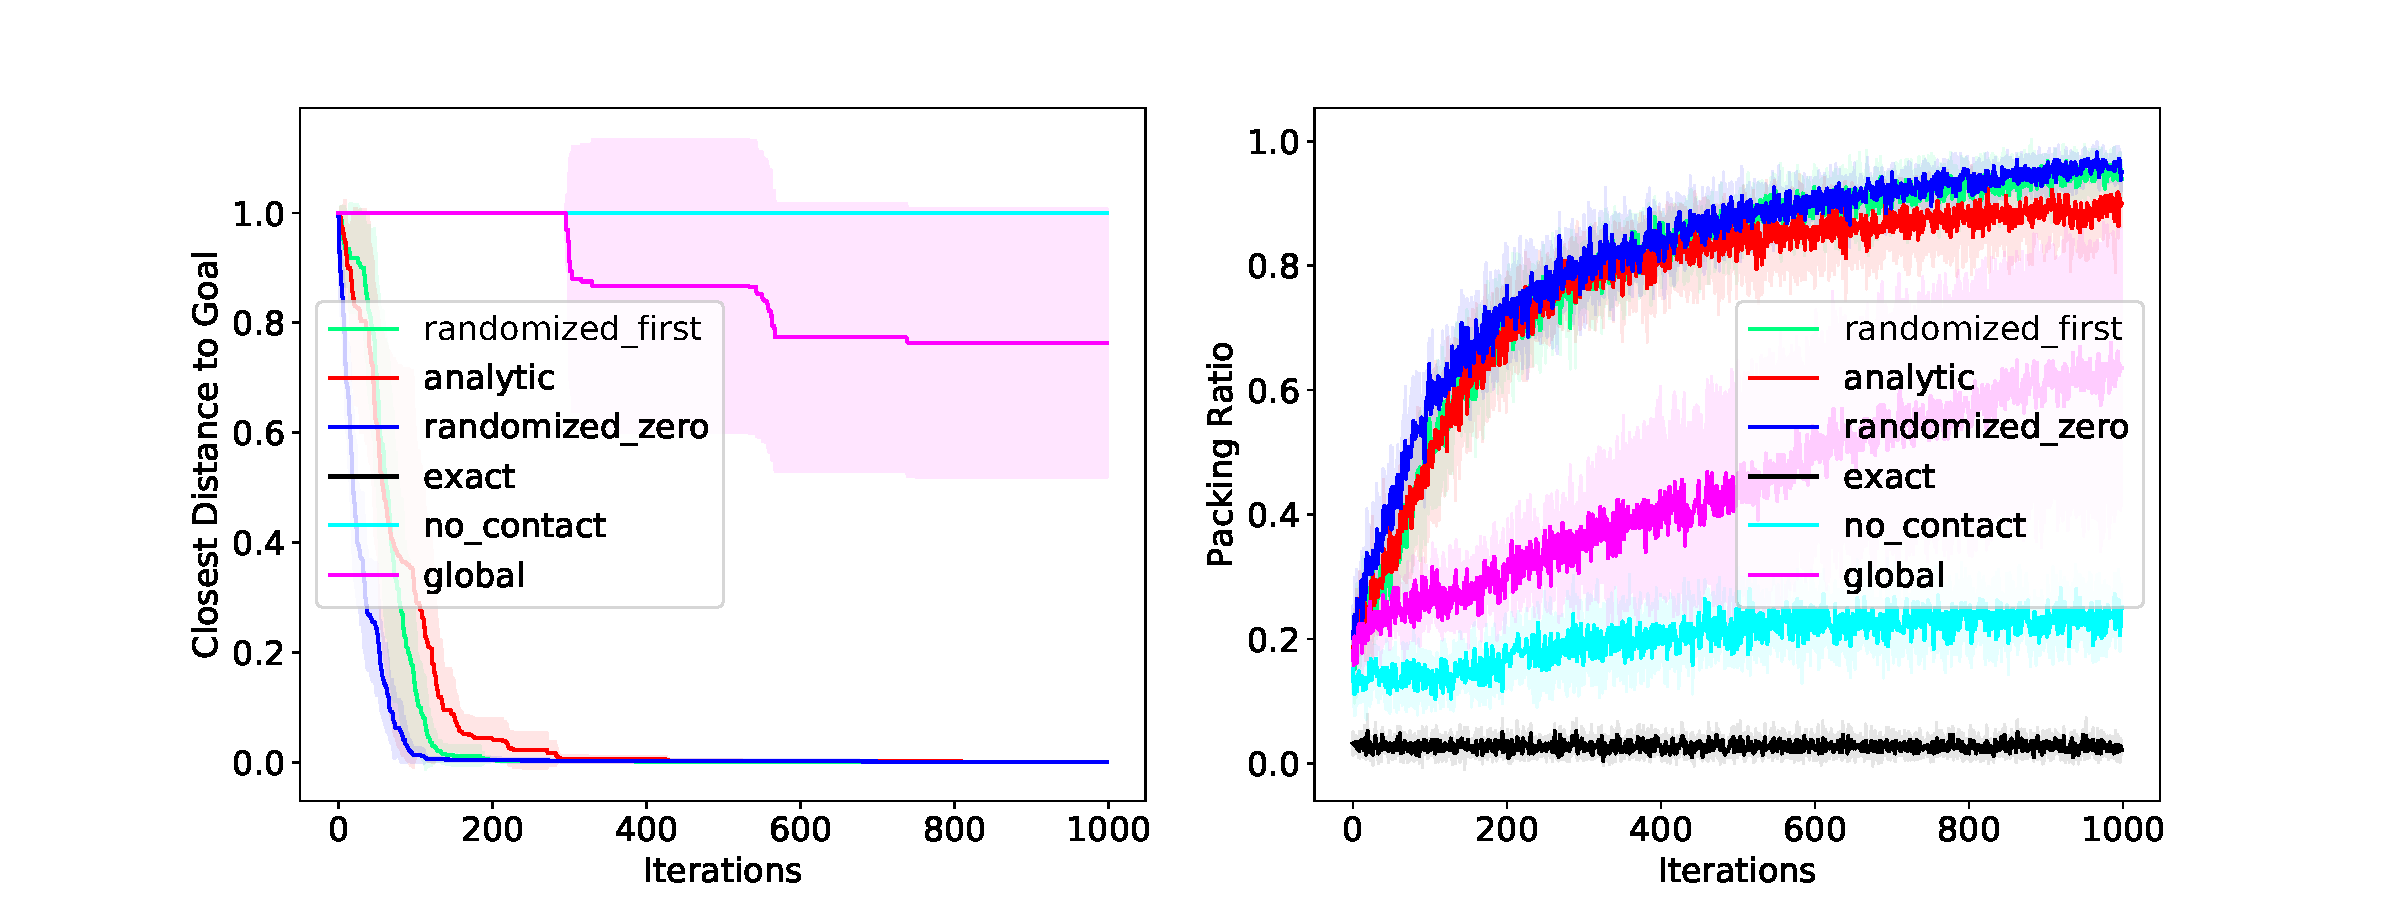
\includegraphics[width=0.485\linewidth]{figures/03_contact_rich_planning/rrt_results/planar_pushing_renamed.pdf}
}
\subfloat[Allegro Plate.]{
	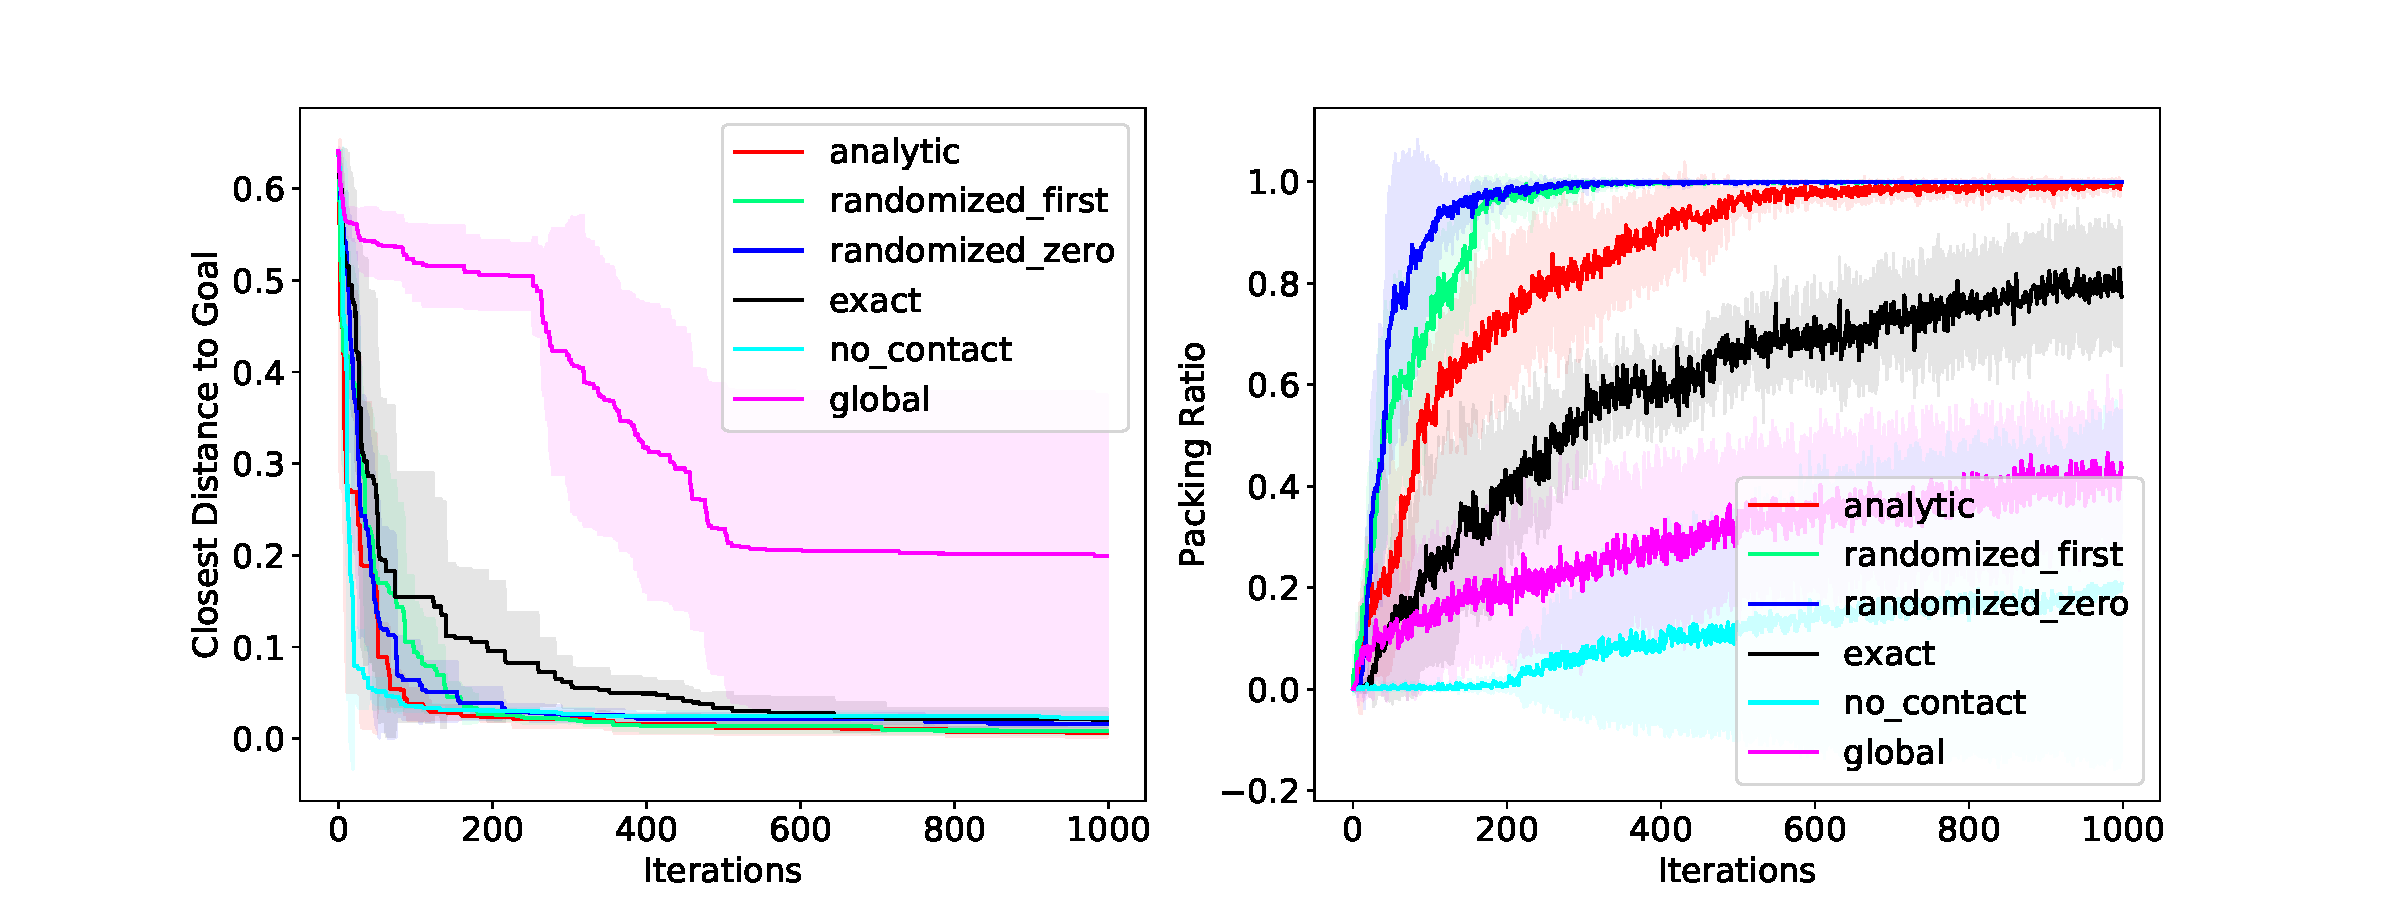
\includegraphics[width=0.485\linewidth]{figures/03_contact_rich_planning/rrt_results/allegrohandplate.pdf}
} \\
\vspace{-0.2cm}
\subfloat[Planar Hand.]{
	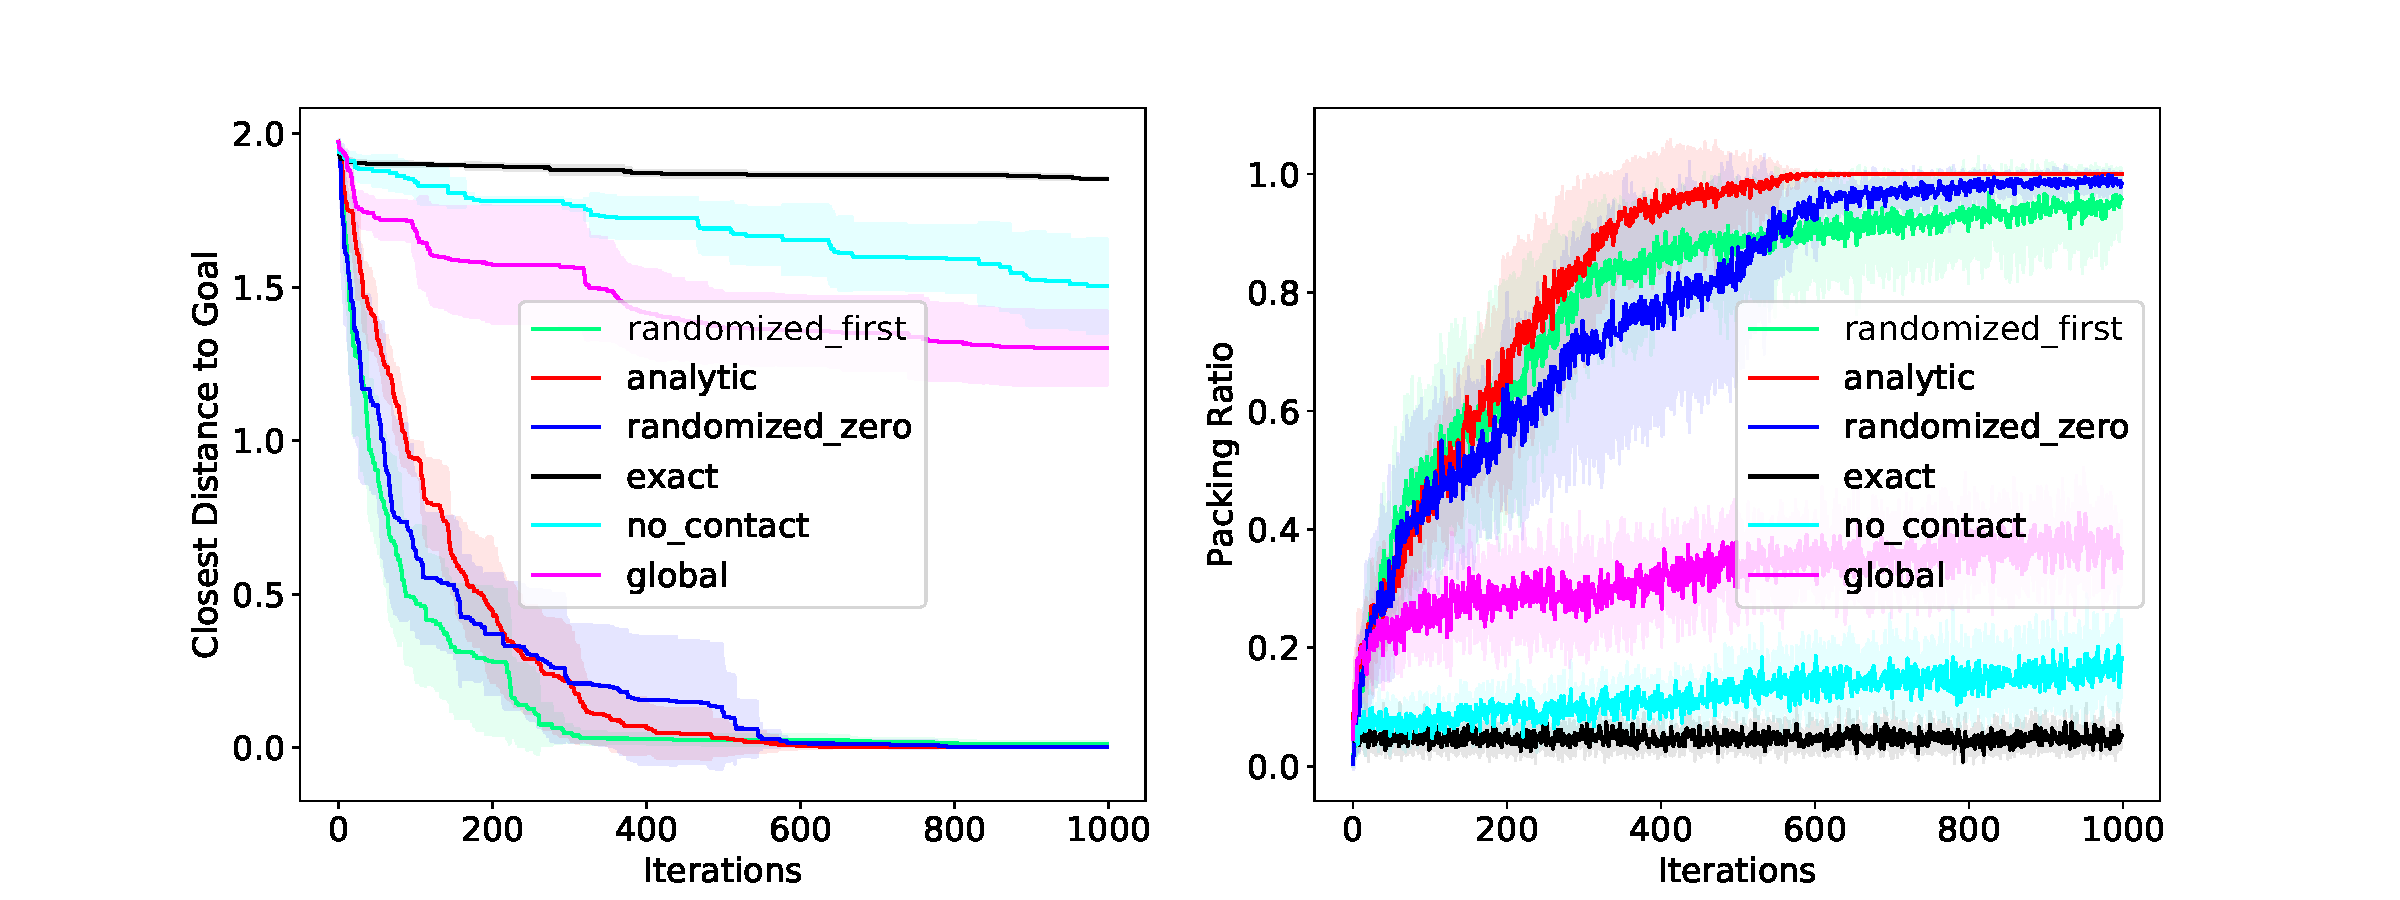
\includegraphics[width=0.485\linewidth]{figures/03_contact_rich_planning/rrt_results/planar_hand_renamed.pdf}
}
\subfloat[Allegro Pen.]{
	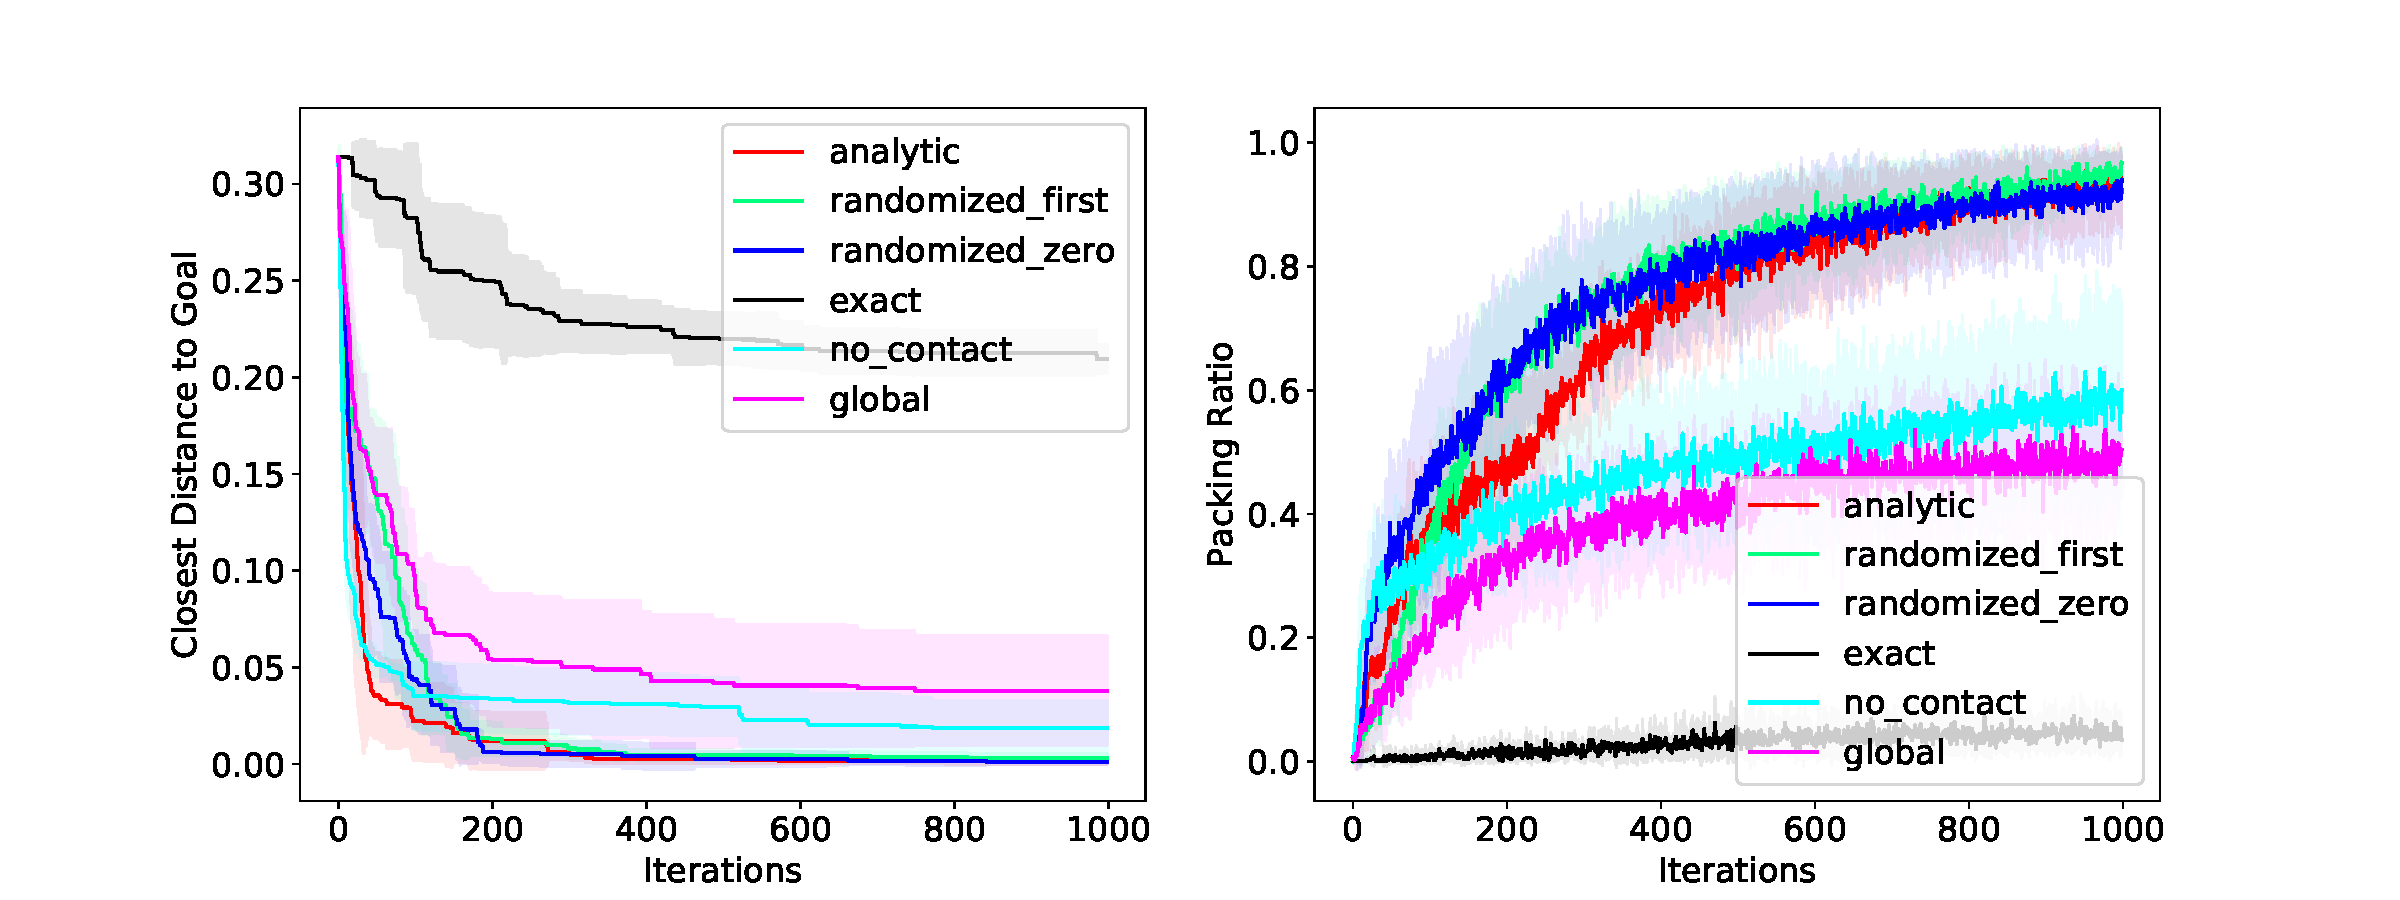
\includegraphics[width=0.485\linewidth]{figures/03_contact_rich_planning/rrt_results/allegrohandpen.pdf}
} \\
\vspace{-0.2cm}
\subfloat[Allegro Hand.]{
	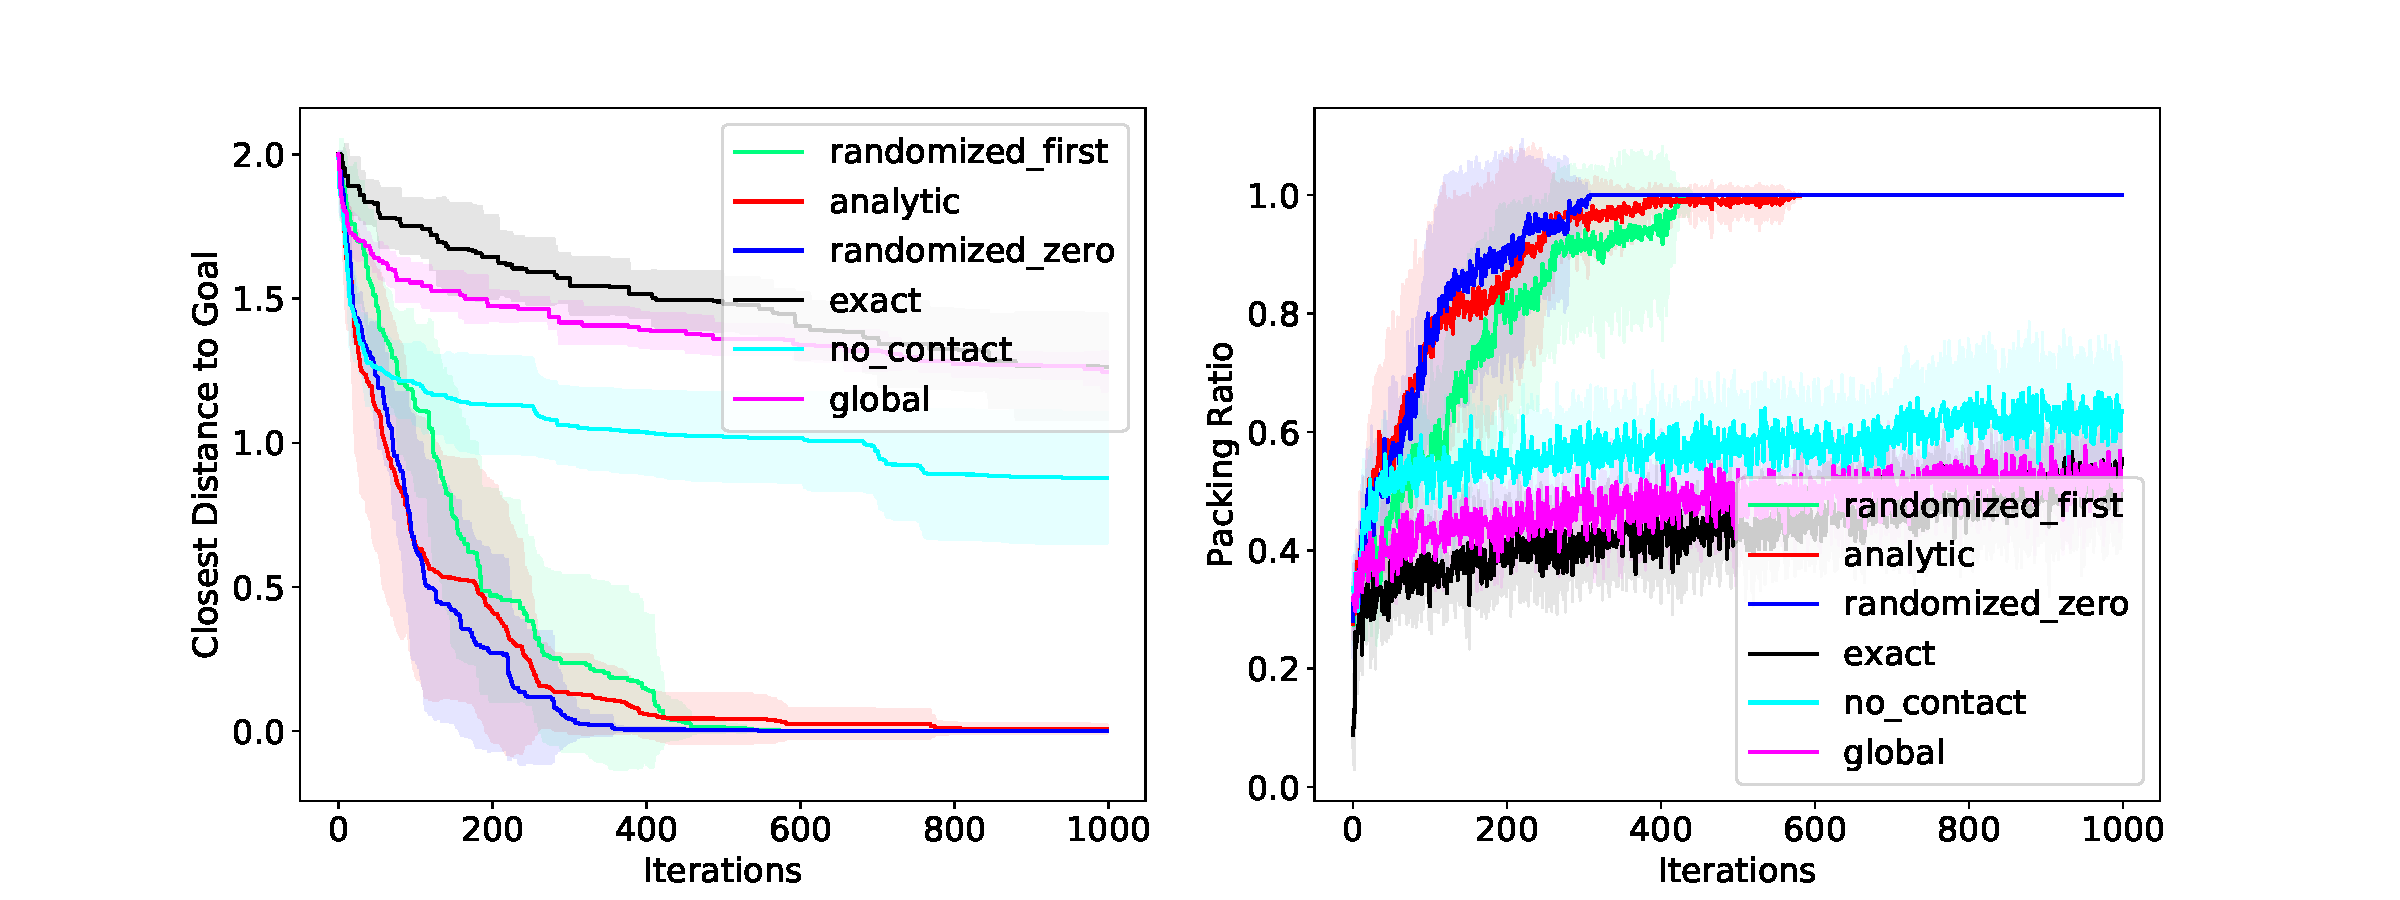
\includegraphics[width=0.485\linewidth]{figures/03_contact_rich_planning/rrt_results/allegrohand.pdf}
}
\subfloat[Allegro Door.]{
	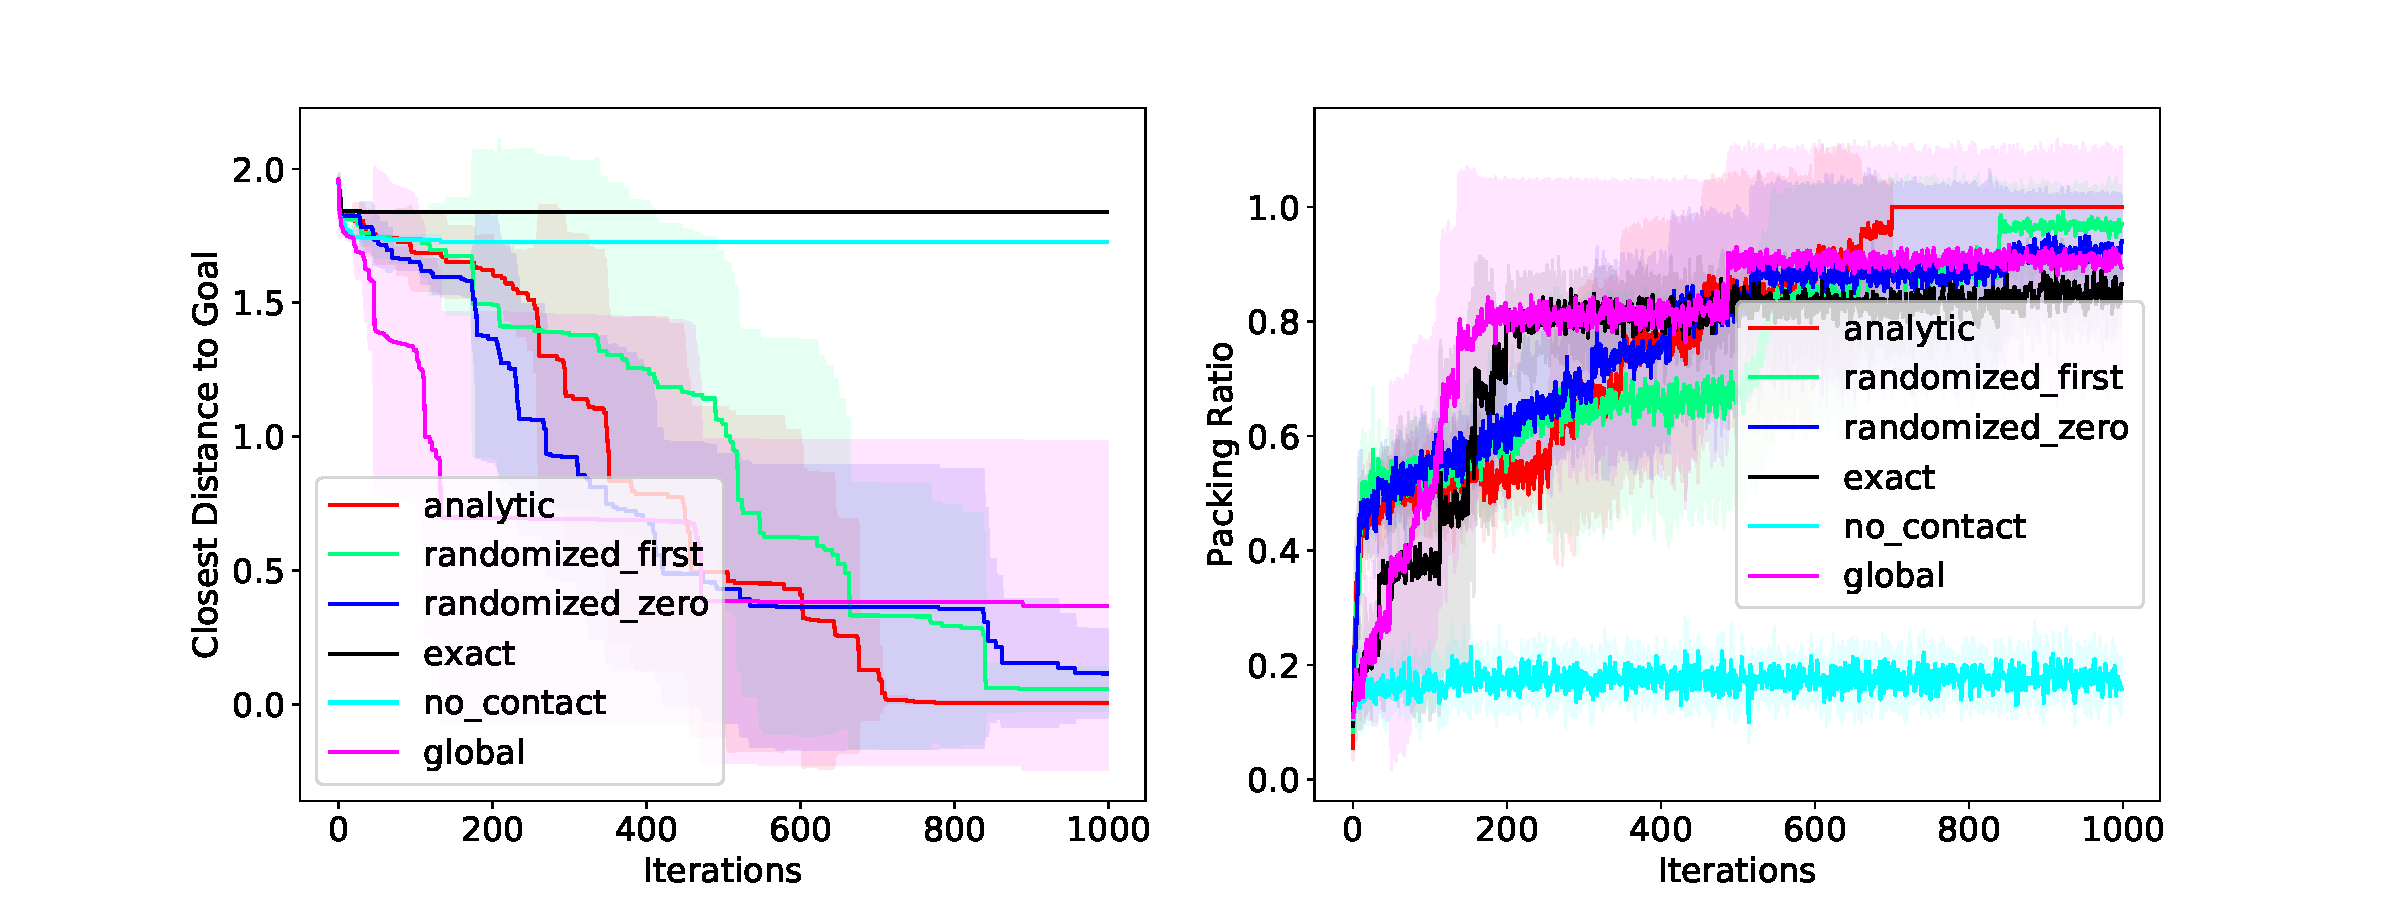
\includegraphics[width=0.485\linewidth]{figures/03_contact_rich_planning/rrt_results/allegrohanddoor.pdf}
}
\caption{Planning performance for the tasks in Fig. \ref{fig:rrt_tasks}. Results include running RRT with the enhancements proposed in Sec. \ref{sec:rrt_for_contact} using the three smoothing schemes from Sec. \ref{sec:smoothdynamics}, as well as the three ablation studies proposed in Sec. \ref{sec:rrt_experiment_setup}.}
\label{fig:rrtperformance}
\end{figure}

\iffalse
\begin{table*}[thpb] \label{tab:trajoptresults}
\centering
\begin{tabular}{|| c | r | r | r | r | r | r || r | r | r | r | r | r || } 
 \hline
 Problem & \multicolumn{2}{||c||}{PlanarPushing} & \multicolumn{2}{||c||}{PlanarHand} & \multicolumn{2}{||c||}{AllegroHand} &
 \multicolumn{2}{||c||}{AllegroPlate} & 
 \multicolumn{2}{||c||}{AllegroPen} & 
 \multicolumn{2}{||c||}{AllegroDoor} 
 \\\hline
 Method & Cost & Time(s) & Cost & Time(s) & Cost & Time(s) & Cost & Time(s) & Cost & Time(s) & Cost & Time(s)  \\ \hline\hline

    Analytic && 3.25  && 10.32 && 31.01 && 117.16 && 24.84 && 12.42  \\
    Randomized  && 7.50 && 21.34 && 80.12 && 161.64 && 86.12 && 34.55\\
    RandomizedZero && 7.40 && 21.00 && 82.00 && 168.11 && 81.23 && 33.80 \\
    Exact && - && - && - && - && - && - \\
    NoContact && - && - && - && - && - && - \\
    Global && - && - && - && - && - && - \\\hline
\end{tabular}
\caption{Minimum cost and running time achieved by different methods. Number of iterations run. Every run except \code{AllegroDoor} was run for $1000$ iterations. We choose to not display running time for the ablation options since they are slight variations of Analytic with comparable running times.}
\label{table:rrtrresults}
\end{table*}
\fi 

For both metrics, the performance of our RRT algorithms averaged over 5 runs is plotted in Fig. \ref{fig:rrtperformance} for different smoothing schemes, as well as ablations of different choices we made for the algorithm. In particular, we run three variations of our algorithm that misses a crucial ingredient.
\begin{enumerate}
    \item \textbf{Exact}. We replace the linearization of the smooth surrogate $\mathbf{B}_\rho$ with the exact linearization $\mathbf{B}$, used for both extension and metric computation.
    \item \textbf{NoContact}. We do not allow contact sampling (Sec.\ref{sec:contactsampling}) in this variant of the algorithm.
    \item \textbf{Global}. Instead of the local Mahalanobis metric, we use a globally uniform metric during the $\Nearest$ step of the algorithm. For our experiments, we use a carefully-chosen weighted Euclidean norm. 
\end{enumerate}
% By showing the results, we aim to show that the choices we made in the design of the algorithm were necessary.


\subsection{Results \& Discussion}

We plot the results of our experiments in Fig. \ref{fig:rrtperformance}, and display the running time of our algorithm using the three different smoothing schemes in Table \ref{table:rrtrresults}. We discuss some of our findings from the experiment, in the context of our hypotheses in the beginning of this section.

\begin{table}[thpb]
\centering
\begin{tabular}{|| c | r | r | r | r | r | r || } 
 \hline
 Method & PPushing & PHand & AHand & APlate & APen & ADoor
 \\\hline
    A. & 3.25  & 10.32 & 31.01 & 117.16 & 24.84 & 12.42  \\
    RF.  & 7.50 & 21.34 & 80.12 & 161.64 & 86.12 & 34.55\\
    RZ. & 7.40 & 21.00 & 82.00 & 168.11 & 81.23 & 33.80 \\\hline
\end{tabular}
\caption{Running time achieved by different methods in seconds. Every trial was run for $1000$ iterations. We choose to not display running time for the ablation options since they are slight variations of Analytic with comparable running times.}
\label{table:rrtrresults}
\end{table}

\subsubsection{Smoothing vs. Exact} Throughout all experiments, we saw that using the exact linearization to compute the distance metric and extension results in much worse performance compared to any of the smoothing schemes, which supports our hypothesis that mode smoothing is necessary in order to solve many of the tasks.

\subsubsection{Analytic vs. Randomized Smoothing} For most of the tasks, we saw no meaningful difference between analytic and randomized smoothing schemes in terms of both how fast the goal is reached and the packing ratio. This empirically supports our theory that the two smoothing schemes are equivalent methods to compute local models of surrogate dynamics. The running time in Table \ref{table:rrtrresults}, however, shows that analytic smoothing results in faster computation time as it does not require taking multiple samples. 

Astute readers might have noticed that in the \code{AllegroPlate} results (Fig. \ref{fig:rrtperformance}b), the packing ratio curve of analytic smoothing lags behind those of both randomized smoothing schemes by a few hundred iterations. First of all, it takes only a few seconds to generate the several hundred samples, so this lag in practice is barely noticeable. 

Nevertheless, we believe the small amount of lag can be attributed to hyper-parameter tuning. For a given amount of smoothing, there is a sweet spot for the step size $h$: if $h$ is too small, RRT makes little progress; if $h$ is too large, RRT takes steps beyond the locality where the smoothed linearization is valid. As the sampling distribution corresponding to a specific $\kappa$ in analytic smoothing is difficult to determine in general,  we usually independently pick the variance for randomized smoothing and the $\kappa$ for analytic smoothing, which means the sizes of the valid regions of the smoothed linearizations under different smoothing schemes can be different. Ideally, we should pick the best $h$ for every smoothing scheme, but in practice we found that an $h$ between $0.1\mathrm{s}$ and $0.2\mathrm{s}$ works reasonably well for all smoothing schemes on all systems. Coming back to the \code{AllegroPlate} example, we believe fine-tuning $h$ for analytic smoothing can remove the lag, but the benefit of doing so is marginal. 

\subsubsection{Global vs. Mahalanobis Metric} Despite reasonable efforts to choose good weights for the weighted Euclidean norm, we consistently observed that the globally uniform weighted Euclidean metric resulted in much worse performance compared to the local Mahalanobis metric. This supports our hypothesis, and the findings of \cite{shkolnik2009reachability} that kino-dynamic RRT in general greatly benefits from guiding tree growth with reachability information. 

\subsubsection{Effect of Contact Sampling} For some of the tasks (e.g. \code{AllegroPlate, AllegroPen}), contact sampling was not necessary. However, for examples that require resetting the actuator into a completely different configuration to make progress (e.g. \code{PlanarPushing, AllegroHand, PlanarHand}), contact sampling greatly improves the planner's performance. 



\section{Sim2Real Transfer \& Hardware Results}\label{sec:sim2real}
Although our planner successfully plans through our CQDC dynamics model, we further investigate if the plans can successfully transfer to real experiments. For this purpose, we run the obtained plans from Sec.\ref{sec:rrt_results} in \emph{open-loop} on a higher fidelity simulator Drake \cite{drake}, as well as an actual hardware setting. These experiments further shed light on the efficacy and the limitations of our proposed method. 

\subsection{Experiment Setup}
\subsubsection{Open-Loop Plan Transfer}
\newcommand{\qsimcoarse}{\{q_{k,\mathrm{sim}}\}^K_{k=0}}
\newcommand{\qsimfine}{\{q_{t,\mathrm{sim}}\}^T_{t=0}}
\newcommand{\ucoarse}{\{u_k\}^{K-1}_{k=0}}

\newcommand{\qsimp}{q_{\mathrm{sim}}}
\newcommand{\qrealp}{q_{\mathrm{real}}}
\newcommand{\qusimp}{q^\mathrm{u}_{\mathrm{sim}}}
\newcommand{\qurealp}{q^\mathrm{u}_{\mathrm{real}}}

Our plan consists of state and action sequences, i.e. lists of ``knot'' points, that are consistent with the CQDC dynamics. We first divide this plan into individual segments $\left(\qsimcoarse, \ucoarse \right)$, punctuated by the $\ContactSample$ operation. 

We convert the knot points $(\qsimcoarse, \ucoarse)$ into state and action trajectories $q_\mathrm{sim}: [0, T] \rightarrow \R[\nU + \nA]$ and $u: [0, T] \rightarrow \R[\nA]$ using first-order hold. Here $T$ denotes the duration of the trajectories in seconds. Specifically, we connect adjacent knot points with linear interpolation for positions and joint angles, or spherical linear interpolation (Slerp) for 3D orientations. The duration of each linear piece is computed such that the robots move at a small and constant speed. Lastly, rolling out $u(\cdot)$ on the real dynamics gives $q_\mathrm{real}: [0, T] \rightarrow \R[\nU + \nA]$, which is compared against $q_\mathrm{sim}(\cdot)$ to evaluate the sim2r

\subsubsection{Evaluation Metrics}
To evaluate the performance of sim2real transfer, we first define the mean error $\Delta(\cdot,\cdot)$ between the two trajectories $q_\mathrm{sim}^\mathrm{u}(\cdot)$ and $q_\mathrm{real}^\mathrm{u}(\cdot)$ as
\begin{equation}
\Delta(q_\mathrm{sim}^\mathrm{u}, q_\mathrm{real}^\mathrm{u}) \coloneqq 
\frac{1}{T}
\int^T_{0} d\left(q_\mathrm{sim}^\mathrm{u}(t), q_\mathrm{real}^\mathrm{u}(t)\right) \mathrm{d}t
\end{equation}
where $d(\cdot,\cdot)$ is the Euclidean 2-norm for position (in meters), and the absolute change in angle for orientation (in radians). Note that for 3D, this change of angle is well-defined in the axis-angle representation. 

In addition, we expect that the metric $\Delta$ will depend on how much movement is inside the reference trajectory of the plan. To account for this scaling, we normalize $\Delta$ by dividing it by the length of the trajectory in the original plan, and denote the normalized error as $\bar{\Delta}$:
\begin{equation}
\bar{\Delta}(\qusimp, \qurealp) \coloneqq 
\frac{\Delta (q_\mathrm{sim}^\mathrm{u}, q_\mathrm{real}^\mathrm{u})}
{L(q_\mathrm{sim}^\mathrm{u})}
,
\end{equation}
where the denominator computes the path length of $q_\mathrm{sim}^\mathrm{u}$: 
\begin{equation}
L(q_\mathrm{sim}^\mathrm{u}) \coloneqq 
\int_0^T \norm{\Dot{q}_\mathrm{sim}^\mathrm{u}(t)}_2 \mathrm{d} t =
\sum^{K - 1}_{k=0}d(q^\mathrm{u}_{k+1,\mathrm{sim}}, q^\mathrm{u}_{k,\mathrm{sim}}).
\end{equation}

This normalization also takes into account the inherent scales of the system, and makes $\bar{\Delta}(\cdot,\cdot)$ a dimensionless quantity. For each system in Fig. \ref{fig:rrt_tasks}, we obtain at least $10$ segments and evaluate our error metrics. 

\subsubsection{Simulation Setup}
We transfer the examples of Fig.\ref{fig:rrt_tasks} into Drake \cite{drake}, which utilizes a full second-order dynamics model with error-controlled integration, as well as a sophisticated and realistic contact model \cite{tamsi}. The collision geometries, robot controller stiffness and coefficients of friction are kept consistent between the CQDC dynamics and Drake. 

\subsubsection{Hardware Setup}
To verify results on actual hardware, we create a variant of the \code{PlanarHand} environment, where the object is replaced by a bucket, and 2 Kuka iiwa arms are used for the actuators. We name this environment \code{IiwaBimanual}. We utilize a motion capture system to estimate the state of the bucket in order to compare the two trajectories of $\qusimp(\cdot)$ and $\qurealp(\cdot)$. Our setup is illustrated in Fig. \ref{fig:hardware}.

\begin{figure}[thpb]
\centering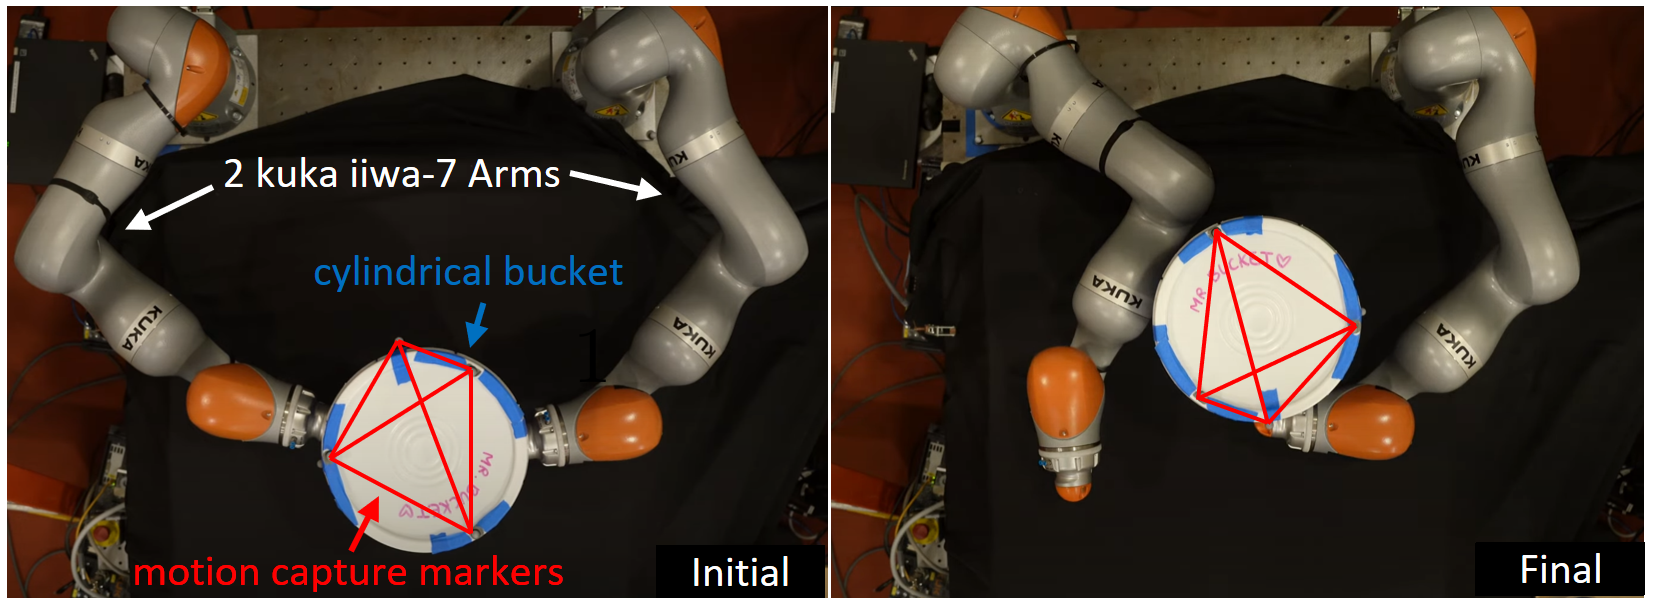
\includegraphics[width = 1.0\linewidth]{figures/03_contact_rich_planning/hardware_setup.png}
\caption{Hardware for the \code{IiwaBimanual} setup, where the goal is to rotate the bucket by $180^\circ$. The left and right pictures correspond to the initial state and the final state after the open-loop plan execution. The lines between motion capture markers are connected to illustrate the change of pose in the bucket. Readers are encouraged to watch the accompanying video for the full execution.} 
\label{fig:hardware}
\end{figure}


\subsection{Results \& Discussion}
We plot the results of our experiments in Fig.\ref{fig:sim_to_real}. While 2D systems such as \code{PlanarPushing}, \code{PlanarHand}, and \code{IiwaBimanual} display low error and good sim2real transfer, 3D systems such as \code{AllegroHand}, \code{AllegroPlate}, \code{AllegroPen} and \code{AllegroDoor} show larger error. To better understand the discrepancy of sim2real performance on different systems, we visualized trajectories from all systems by overlaying $\qurealp$ on top of $\qsimp$ (some of these visualizations are shown in the accompanying video). 

\begin{figure*}[thpb]
\centering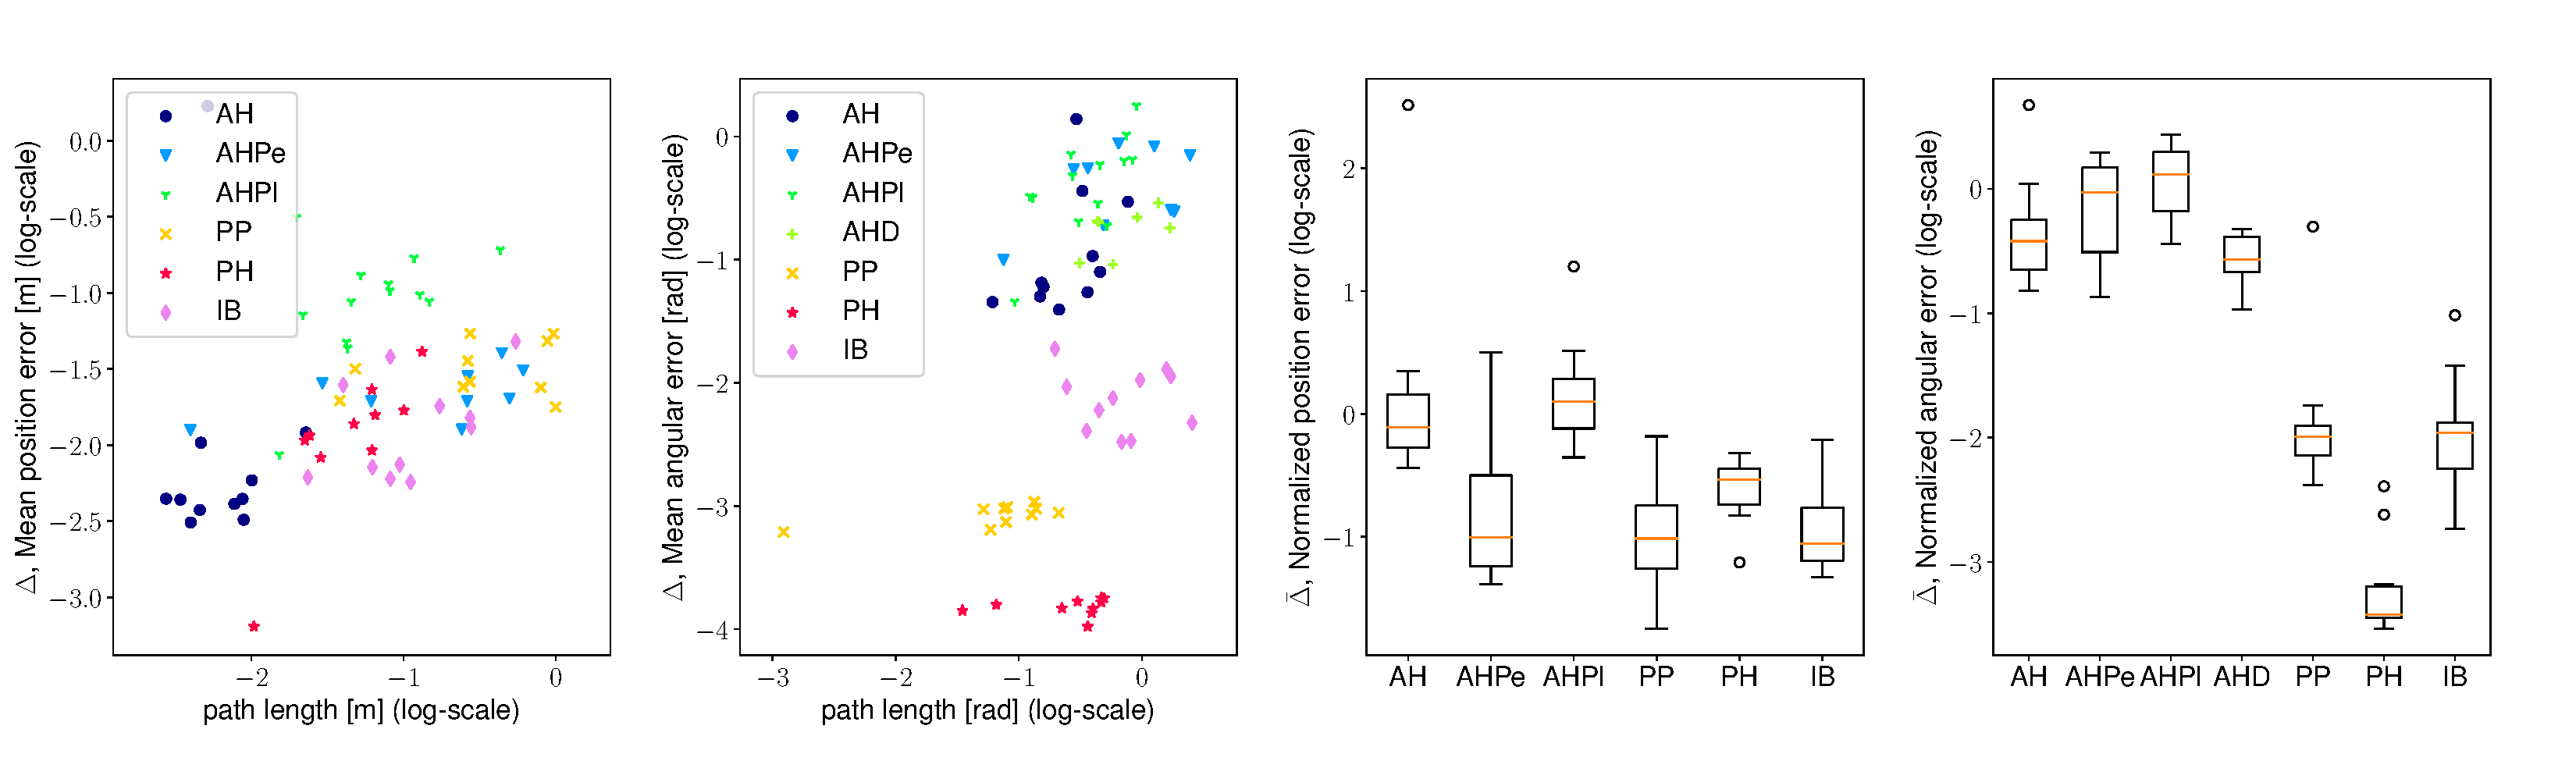
\includegraphics[width = 1.0\linewidth]{figures/03_contact_rich_planning/sim_to_real.pdf}
\caption{Plots for sim2real performance of our CQDC dynamics, evaluated on the plans of Sec.\ref{sec:rrt_results}. \textbf{First Two Columns}: Scatter plot of mean error $\Delta$ vs. path length for position (first column) and orientation (second column). Each dot in the plot represents one segment trajectory. \textbf{Last Two Columns}: Box plot for the normalized error $\bar{\Delta}$ for positions (third column) and orientation (fourth column). Note that the mean in orange corresponds to the slope of the graph in the first two columns. Finally, we note that the \code{AllegroHandDoor} (AHD) example only consists of orientation, and has no position plot. Readers are highly encouraged to watch the accompanying video for the qualitative behavior of the actual segment trajectories in this plot.}
\label{fig:sim_to_real}
\end{figure*}

From the video, it is clear that on \emph{all} systems, there exists a persistent \emph{phase} difference between $\qurealp$ and $\qusimp$: $\qurealp$ tends to lag $\qusimp$ when the robot accelerates, and lead when the robot decelerates. This is not surprising, as the CQDC dynamics that generates $\qusimp$ is inherently a first-order system, whereas $\qurealp$ is generated from second-order dynamics. 
On trajectory segments with good sim2real performance, the phase gap only results in harmless oscillations of $\qurealp$ around $\qusimp$. In these cases, we believe that the good sim2real performance validates our contact model. 
However, the phase gap can have more serious consequences, which we will discuss next.


\subsubsection{Violation of Quasi-static Assumption} 
The quasi-static assumption implies that objects are quickly stopped by damping when they are not ``pushed around'' by the robot. This is true on 2D systems, as the friction patch between the object and its supporting surface is persistent and always provides enough damping to bring the object to still. 

However, the necessary damping to uphold the quasi-static assumption does not always exist on 3D systems. For instance, in \code{AllegroHand} and \code{AllegroHandPen}, the point contact between the object and the palm provides very little damping. Most of the damping comes from the finger joints when the fingers are opposing the object's motion. Therefore, when the grasp on the object ``leaves an opening'', the object can roll quite far from the planned trajectory or even off the palm. 

\subsubsection{Missed Contacts}
Due to the non-smooth nature of contact dynamics, small discrepancies in object trajectory caused by the phase gap can lead to the robot completely missing contacts with the object. For example, we observed that in \code{AllegroHandPlate} or \code{AllegroHandDoor}, some grasps that were valid under the CQDC dynamics no longer succeeded in holding the object in place in Drake. The consequence of these failed grasps is that plates are dropped on the table in \code{AllegroHandPlate}, and door handles are missed in \code{AllegroHandDoor}.


\subsubsection{Necessity of Stabilization \& Robustification}
These results tell us that the plan suggested by the CQDC dynamics might give a high-level direction, but its open-loop execution may not succeed under second-order dynamics with high velocities and low amount of damping. We believe that tracking this high-level plan requires low-level feedback controllers that can stabilize to the plan, and actively enforce the closed-loop system to be quasi-static. We also believe that the high-level planer can benefit from robustness objectives such as encouraging grasps that are considered good under classical grasping metrics. Such grasps will increase the control authority of the robot over the object, thereby providing sufficient damping and decreasing the chances of dropping the object. We leave these as promising directions for future work. 
\chapter{External Contact Detection from Joint Torque Measurements} \label{chapter:force_from_torque}
\section{Introduction}
No longer confined to factory-floor workcells repeating painstakingly hand-coded trajectories, robot arms today have been tasked with increasingly open-ended assignments such as ``put this shoe on the shelf'' or ``load the dish washer'', where the robots need to operate in unknown, unstructured environments potentially populated by humans. Naturally, the safety of such operations hinges upon the robot's ability to reliably handle unplanned collisions between any part of itself and the environment. 

The ultimate sensor for collision detection is perhaps a sensitive tactile skin covering the entire surface of the robot \cite{cannata2008embedded, jain2013reaching}. However, such skins are rarely seen outside research labs, as they are usually expensive and prone to wear and tear. On the other hand, joint-level proprioceptive torque sensors are mature, robust and becoming more common in robot arms designed for human-robot interactions \cite{loughlin2007dlr, franka}.

Several techniques have been developed to estimate both the external contact force and its location on the whole robot using only proprioceptive torque sensors \cite{haddadin2017robot, manuelli2016localizing, zwiener2018contact, zwiener2019armcl}. However, due to the sparse nature of proprioceptive measurements (one torque measurement per link), estimation of contact force and location from only joint torque has obvious limitations. For a typical serial robot arm with 7 links, when link $i$ (numbered from the base) of the arm is in contact, there are $i$ torque measurements available, and $i \leq 6$ if the contact is not on the end effector. The fact that the contact is pushing the robot gives two additional constraints: the force being in the friction cone and the position being on the robot's surface. In contrast, a contact position has 3 independent components to estimate, and a contact wrench has 6. As a result of this deficiency in available measurements, the literature on joint-torque-based contact estimation commonly assumes that (\textbf{i}) there exists at most one external contact, and (\textbf{ii}) the contact generates negligible moments at the contact point \cite{haddadin2017robot, zwiener2019armcl}.

\begin{figure}
\centering
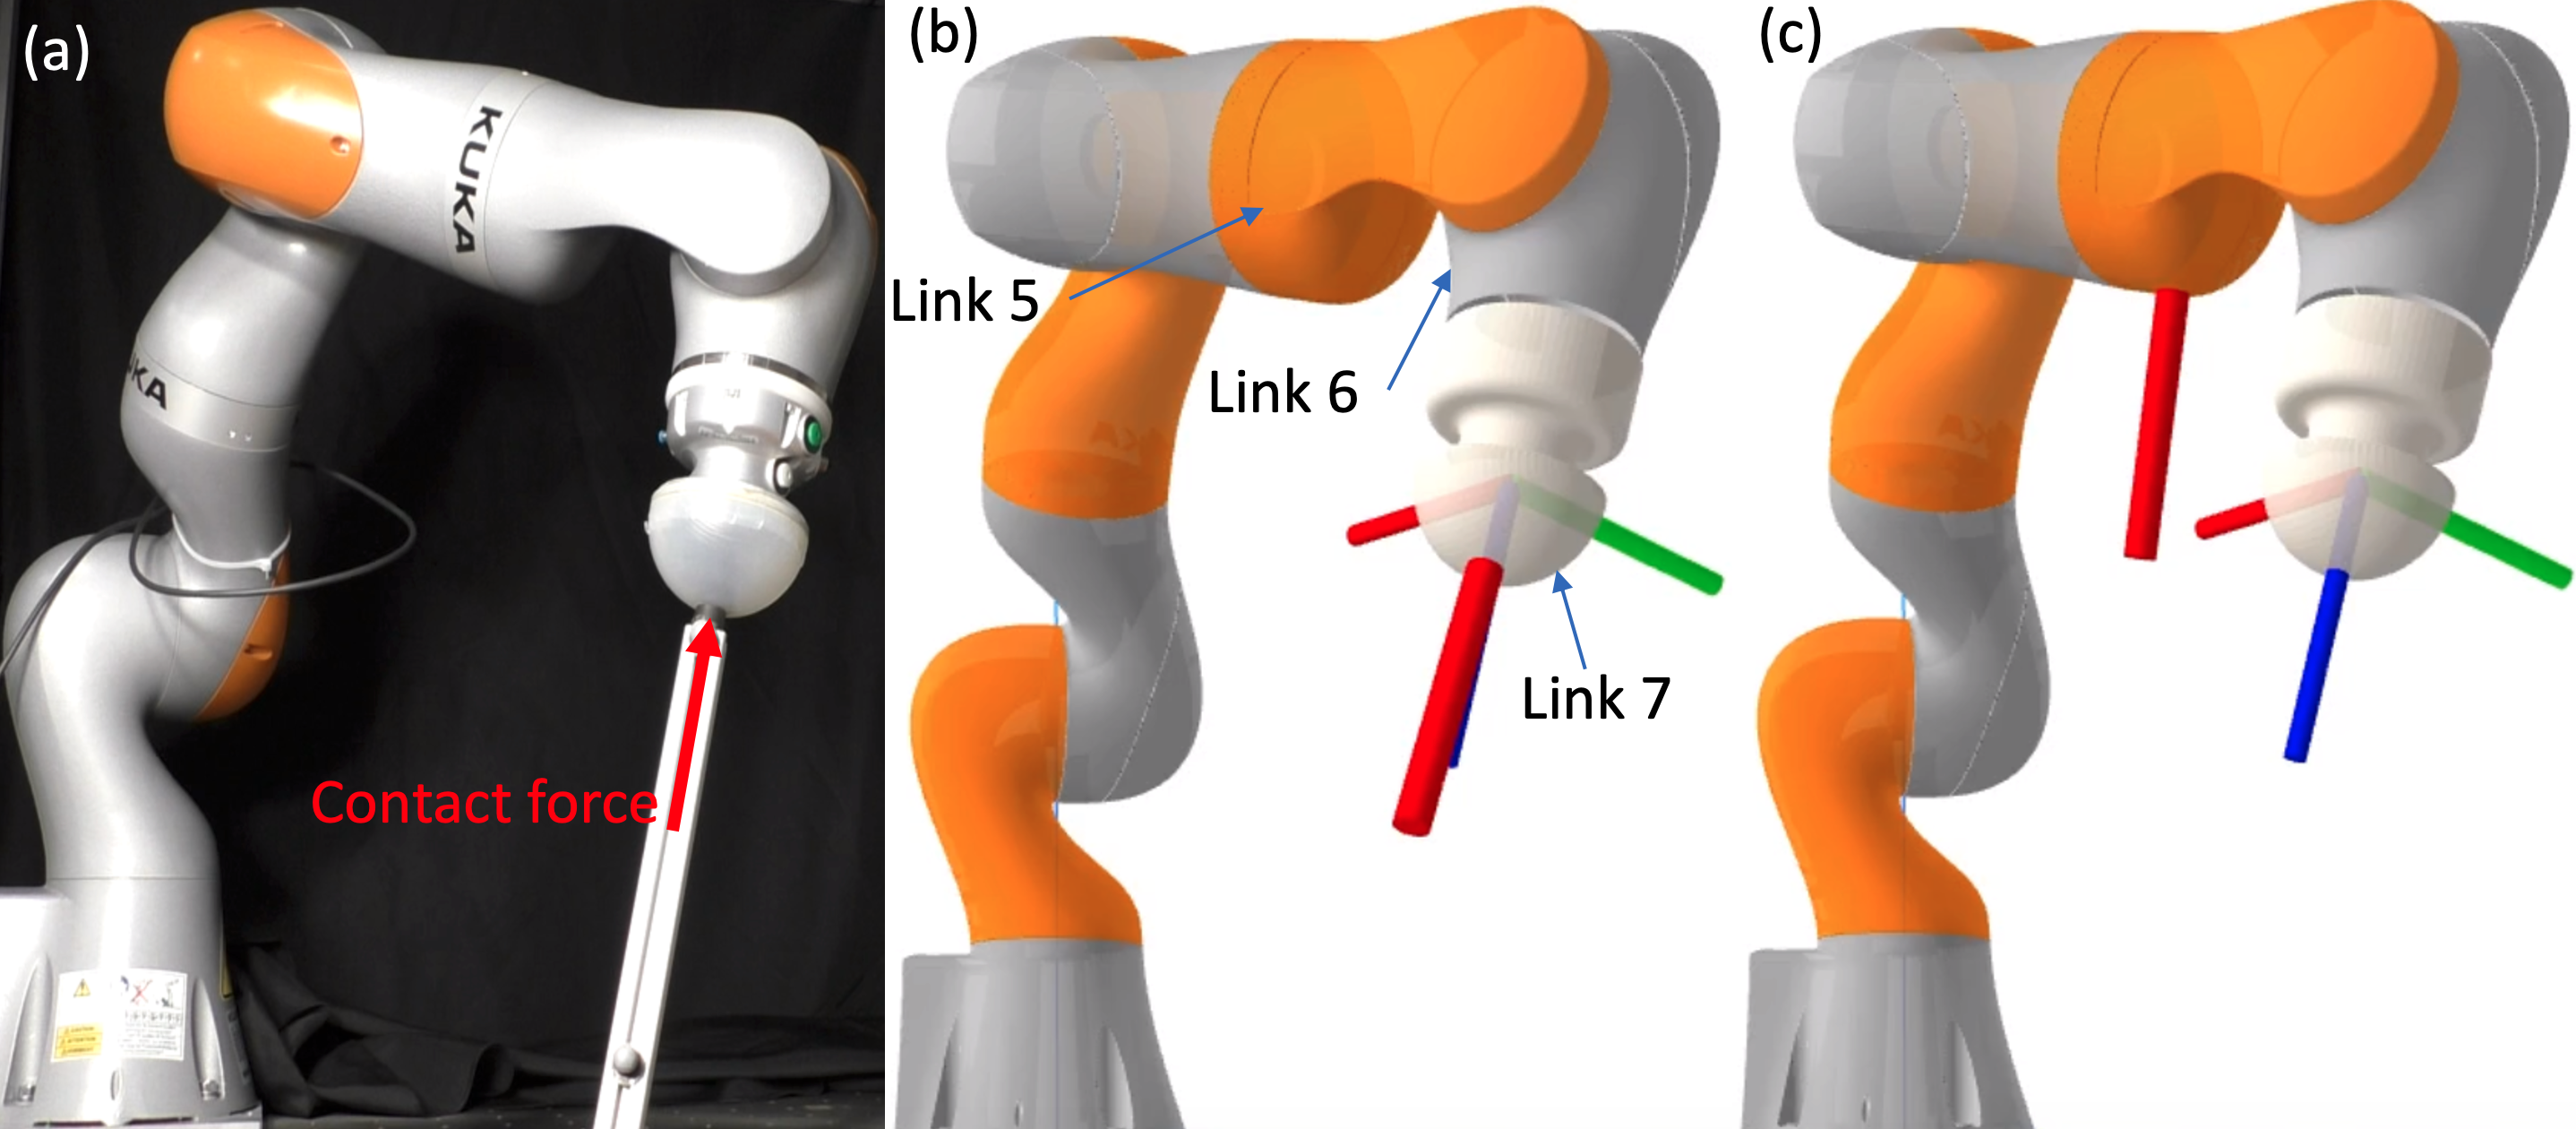
\includegraphics[width=0.9\linewidth]{figures/05_force_from_torque/cpf_failure.png}
\caption{For the true contact shown in (\textbf{a}), which generates little torque about joint 6 and 7, the two contacts in (\textbf{b}) and  (\textbf{c}), represented by red cylinders, create almost identical torque measurements as (\textbf{a}).}
\label{fig:cpf_failure}
\end{figure}

However, even within the boundary set by these simplifying assumptions, joint-torque-based contact estimation is still limited by the loss of detectability of contacts from joint torque measurements, which we will discuss more formally in Section. \ref{sec:observability}. Intuitively, as shown in Fig. \ref{fig:cpf_failure}, it is likely that multiple contact positions and forces (Fig. \ref{fig:cpf_failure}b and \ref{fig:cpf_failure}c) create almost identical torque measurements, making them impossible to distinguish by looking at joint torque alone. Although this failure mode has been observed in existing work \cite{zwiener2018contact}, a thorough analysis on how often joint-torque-based contact estimators fail and what can be done to mitigate such failures appears to be absent from the literature. 

In this chapter, we show quantitatively that two distinct contacts generating almost identical joint torque measurements is far from a 0-probability event. Moreover, this probability can get alarmingly high for links whose geometry is ``concentrated'' around their joint axes, such as links of the IIWA arm. Therefore, we believe that solving for a single contact estimate from joint torque measurements is an inadequate problem formulation. Instead we propose to estimate the \emph{set} of possible contact positions consistent with the measurements.  Elements of this set can be cast as the global optimal solution of a nonlinear optimization problem, which is difficult to solve directly. Nevertheless, by combining rejection sampling and gradient descent on manifolds, we propose an estimator that searches for local minima of the nonlinear optimization problem, and provide an efficient implementation capable of running at real-time rates. In practice, the proposed estimator usually finds all local minima on the links it searches. In addition, given the set of possible contact positions, we also propose an active contact discrimination strategy that falsifies spurious contact positions by slightly moving the robot.


%%%%%%%%%%%%%%%%%%%%%%%%%%%%%%%%%%%%%%%%%%%%%%%%%%%%%%%%%%%%%%%%%%%%%%%%%%%%%%%%
\section{Related Work}
Although raw measurements from joint torque sensors include gravitational and inertial effects, the torque generated by external contacts, also known as the residual torque, can be extracted from them using external torque observers \cite{haddadin2017robot}. Having become an integral part in many robot arms' firmware \cite{loughlin2007dlr, franka}, such observers can update residual torque estimates at hundreds of Hz, providing the foundation for all proprioceptive contact estimation methods.

The contact estimator by Haddadin \textit{et al.} \cite{haddadin2017robot} first determines the link in contact as the last link with non-zero residual torque. It then solves for the line of action of the contact force from a system of linear equations relating torque measurements to the contact wrench. Finally, if the contact geometry of the link is convex, intersecting the line with the link will give two potential contact points, one for pulling and the other for pushing. As contact forces almost always push, the contact point can thus be uniquely determined. However, solving for the line of force action needs at least 6 torque measurements and a full-rank contact Jacobian, which implies this method does not produce any outcome on links more proximal to the base than link 6 or when the robot is close to singular. Moreover, when a link is not convex (e.g. link 5 in Fig. \ref{fig:cpf_failure}), the line of force action may intersect the link at more than two locations, making it impossible to uniquely determine the contact point.

Methods based on the Markov Chain Monte Carlo (MCMC) methodology \cite{manuelli2016localizing, zwiener2019armcl} can theoretically work on any link and with rank-deficient contact Jacobians, although estimation accuracy typically degrades on links too close to the base, or when the robot is close to singular. The degradation is not a limitation of the methods themselves, but a result of the loss of detectability of contacts from joint torque measurements. Both \cite{manuelli2016localizing} and \cite{zwiener2019armcl} use random walk on the robot's surface as the proposal distribution, and evaluate the likelihood of samples using the L2 norm of the difference between the measured joint torque and the joint torque created by the sample. The difference is that \cite{manuelli2016localizing} assumes frictional contacts whereas \cite{zwiener2019armcl} assumes that contacts are frictionless. The biggest drawback of MCMC methods is that they typically converge to only one local minima of the likelihood function, and are oblivious of other local minima when they exist.

Proprioceptive contact estimator based on machine learning has also been explored. Zwiener \textit{et al.} discretize a robot's surface into finitely many patches, and train a classification network to predict the patch in contact from joint torque \cite{zwiener2018contact}. Although the contact classifier works well on both the training and validation data sets, its limitations and failure modes are difficult to analyze; its ability to generalize beyond the data set it is trained on is also hard to gauge. 

%%%%%%%%%%%%%%%%%%%%%%%%%%%%%%%%%%%%%%%%%%%%%%%%%%%%%%%%%%%%%%%%%%%%%%%%%%%%%%%%
\section{Problem Formulation \label{sec:problem_statement}}
For given joint angles $q \in \mathbb{R}^{n_q}$ and residual joint torque $\tauE \in \mathbb{R}^{n_q}$ created by one external contact at point $C$, the problem is to find $p_C \in \mathbb{R}^3$, the coordinate of contact point $C$, and the contact force $f_C$. In other words, we would like to solve for $p_C$ and $f_C$ from the following equation:
\begin{equation}
\label{eq:torque_jacobian_force}
\tauE = {J}_C({q}, {p}_C)^\intercal {f}_C,
\end{equation}
where ${J}_C({q}, {p}_C) \in \mathbb{R}^{3 \times n_q}$ the contact Jacobian that maps joint velocity $\dot{q}$ to the velocity of $C$. 

As shown in Fig. \ref{fig:friction_cone}a, $C$ is confined to the robot's surface, and the contact force ${f}_C$ needs to stay inside the friction cone at $C$: $\norm{{f}_{C_f}} \leq \mu \norm{{f}_{C_n}}$. The second-order cone can be approximated with the polyhedral cone in Fig. \ref{fig:friction_cone}b, which is generated by a set of $n_d$ extreme rays ${v}_C = \{{v}_{C_1}, \dots, {v}_{C_{n_d}}\}$, such that ${f}_C = \sum_{i=1}^{n_d} {v}_{C_i} \beta_i = {v}_C {\beta}$ with $\beta_i \geq 0$ \cite{stewart2000implicit}.    

\begin{figure}[h]
\centering
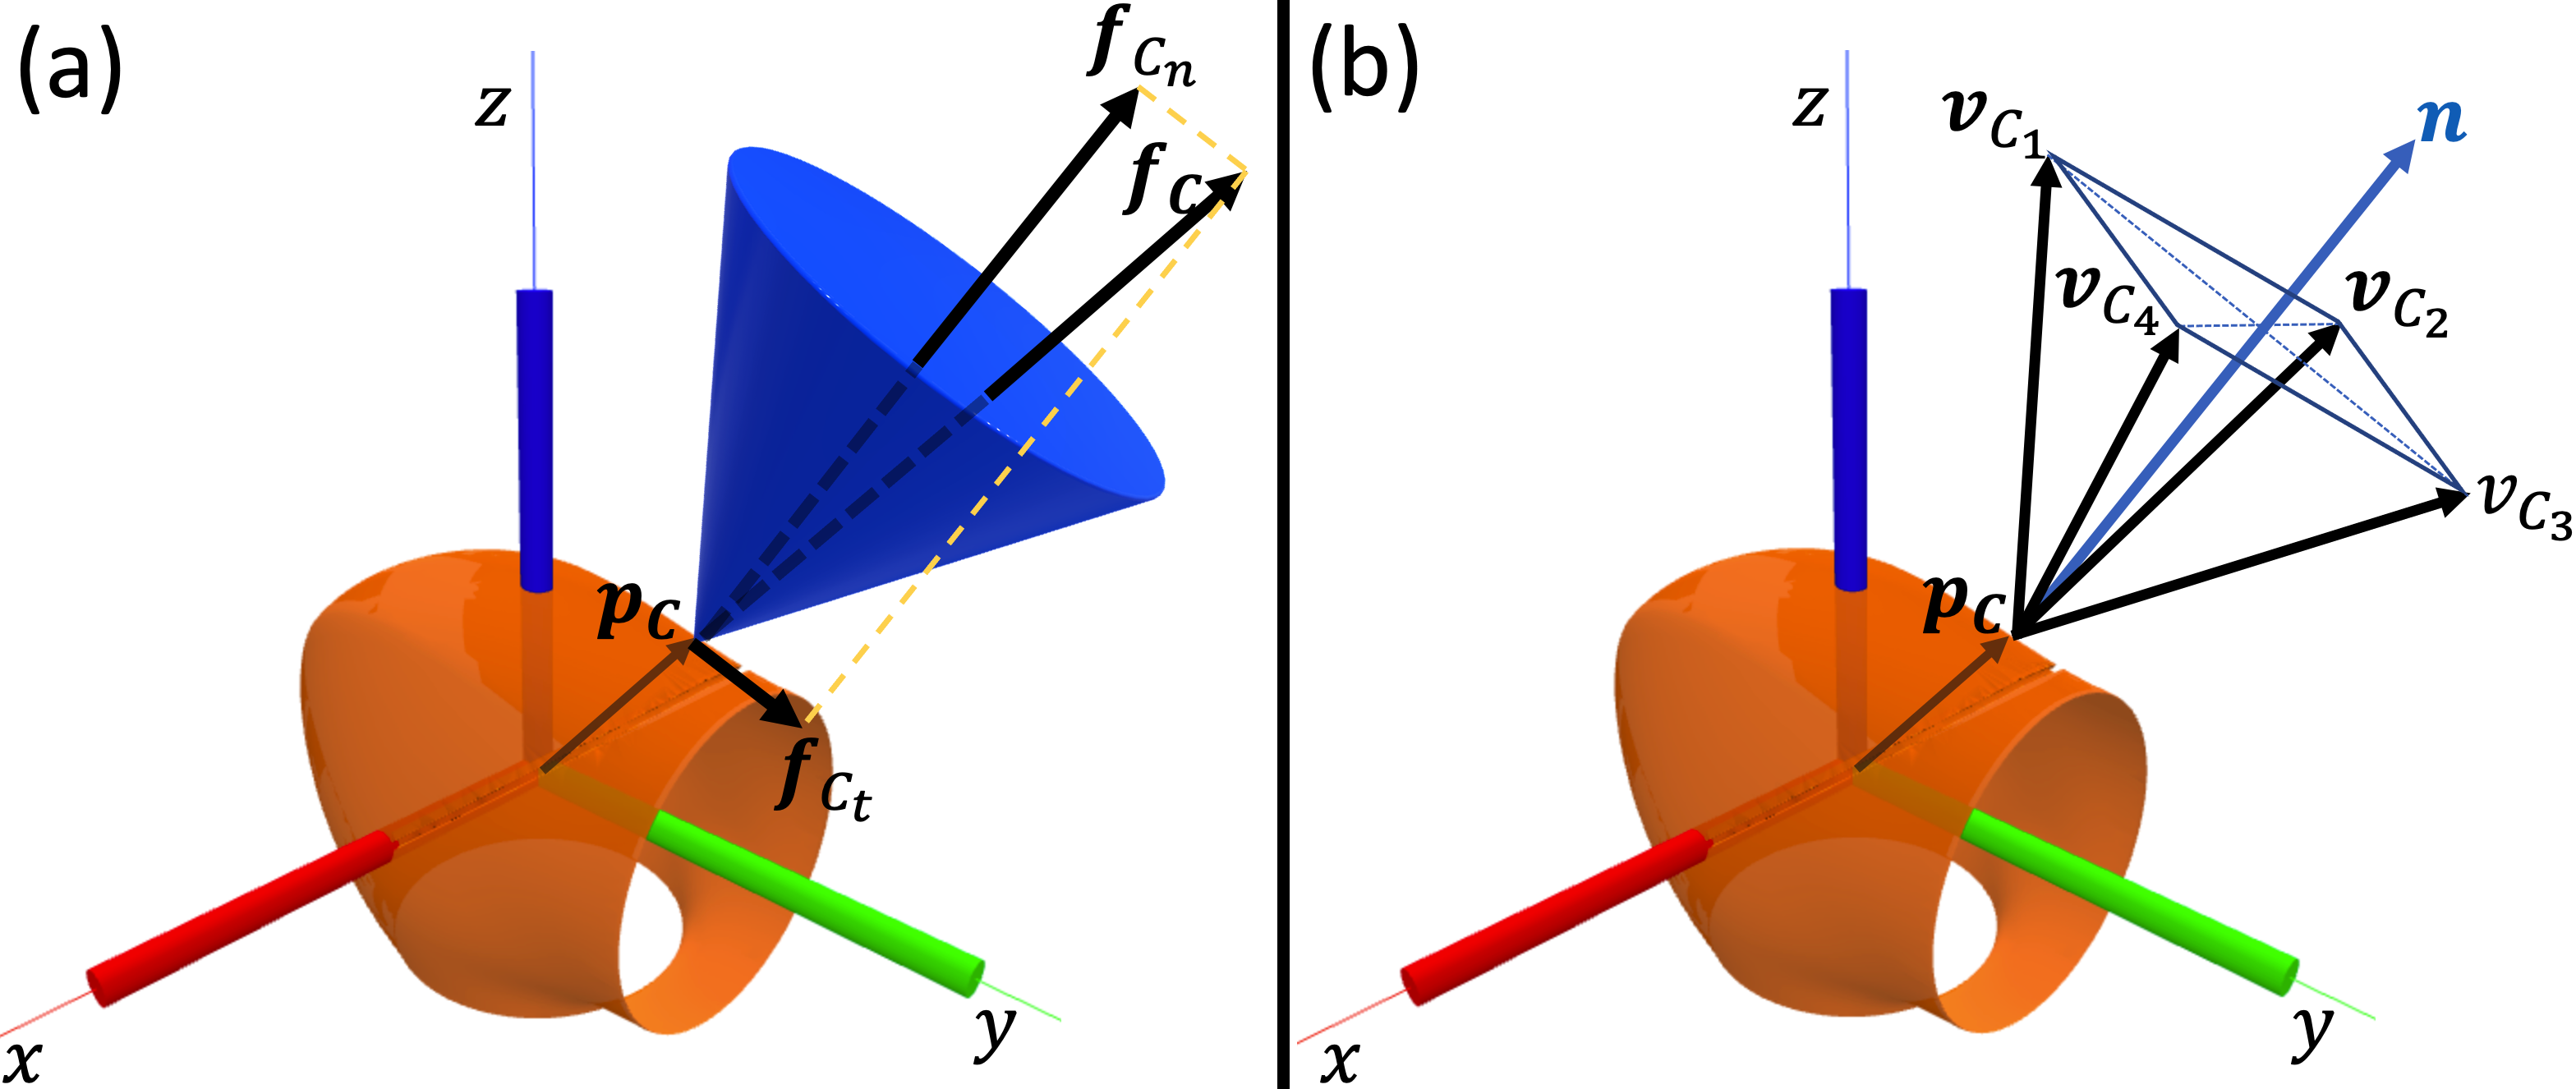
\includegraphics[width=0.98\linewidth]{figures/05_force_from_torque/friction_cone.png}
\caption{A contact force on Link 6 of the KUKA IIWA robot. The orange mesh is the surface of the link. The triad represents the body frame of the link. (\textbf{a}) second-order friction cone. (\textbf{b}) Polyhedral approximation of the friction cone with $n_d=4$.}
\label{fig:friction_cone}
\end{figure}

Solving (\ref{eq:torque_jacobian_force}) with the friction cone constraint is equivalent to solving the following optimization problem:
\begin{equation}
\label{eq:nonlinear_program}
\underset{{\beta} \geq 0, \; \pCbar \in \mathcal{S}}{\text{min.}} \; \| {J}({q}, \pCbar)^{\intercal} {\beta} - {\tau}_\text{ext} \|^2,
\end{equation}
where ${J}({q}, \pCbar) = {v}_C^\intercal {J}_C({q}, \pCbar) \in \mathbb{R}^{n_d \times n_q}$, and $\mathcal{S}$ is the manifold of the robot's surface. The overbar in $\pCbar$ emphasizes that the solution to (\ref{eq:nonlinear_program}) can be different from the actual ${p}_C$. For fixed ${q}$ and $\tauE$, a contact position estimate $\pCbar$ has an associated cost defined as
\begin{subequations}
\label{eq:residual_qp}
\begin{align}
l(\pCbar; {q}, \tauE) \coloneqq& \underset{{\beta} \geq 0}{\text{min.}} \; \| {J}({q}, \pCbar)^{\intercal} {\beta} - {\tau}_\text{ext} \|^2 \\
=& \underset{{\beta} \geq 0}{\text{min.}} \left({\beta}^\intercal \underbrace{{J}{J}^\intercal}_{\mathbf{Q}} {\beta} - 2 \left(\underbrace{{J} \tauE}_{-{b}}\right)^\intercal {\beta} + \tauE^\intercal \tauE \right). \label{eq:residual_qp:qp}
\end{align}
\end{subequations}
The function $l(\; \cdot \;; {q}, \tauE): \mathbb{R}^3 \rightarrow \mathbb{R}$ is also called the \textit{residual}, and can be computed by solving (\ref{eq:residual_qp:qp}), which is a convex QP. Using $l(\cdot)$, the set of solutions of (\ref{eq:nonlinear_program}) can be described by the set
\begin{equation}
P_0(q, \tauE) \coloneqq \{\pCbar \in \mathcal{S} : l(\pCbar; q, \tauE) = 0\}.
\end{equation}

The true contact location ${p}_C$ is clearly in $P_0(q, \tauE)$. However, it is possible that $|P_0| > 1$, i.e. different contact forces at different positions can generate the same joint torque $\tauE$, as shown in Fig. \ref{fig:multiple_local_minima}. In general, it is not possible to distinguish ${p}_C$ from other elements of $P_0(q, \tauE)$ using only $q$ and $\tauE$.

\begin{figure}[h]
\centering
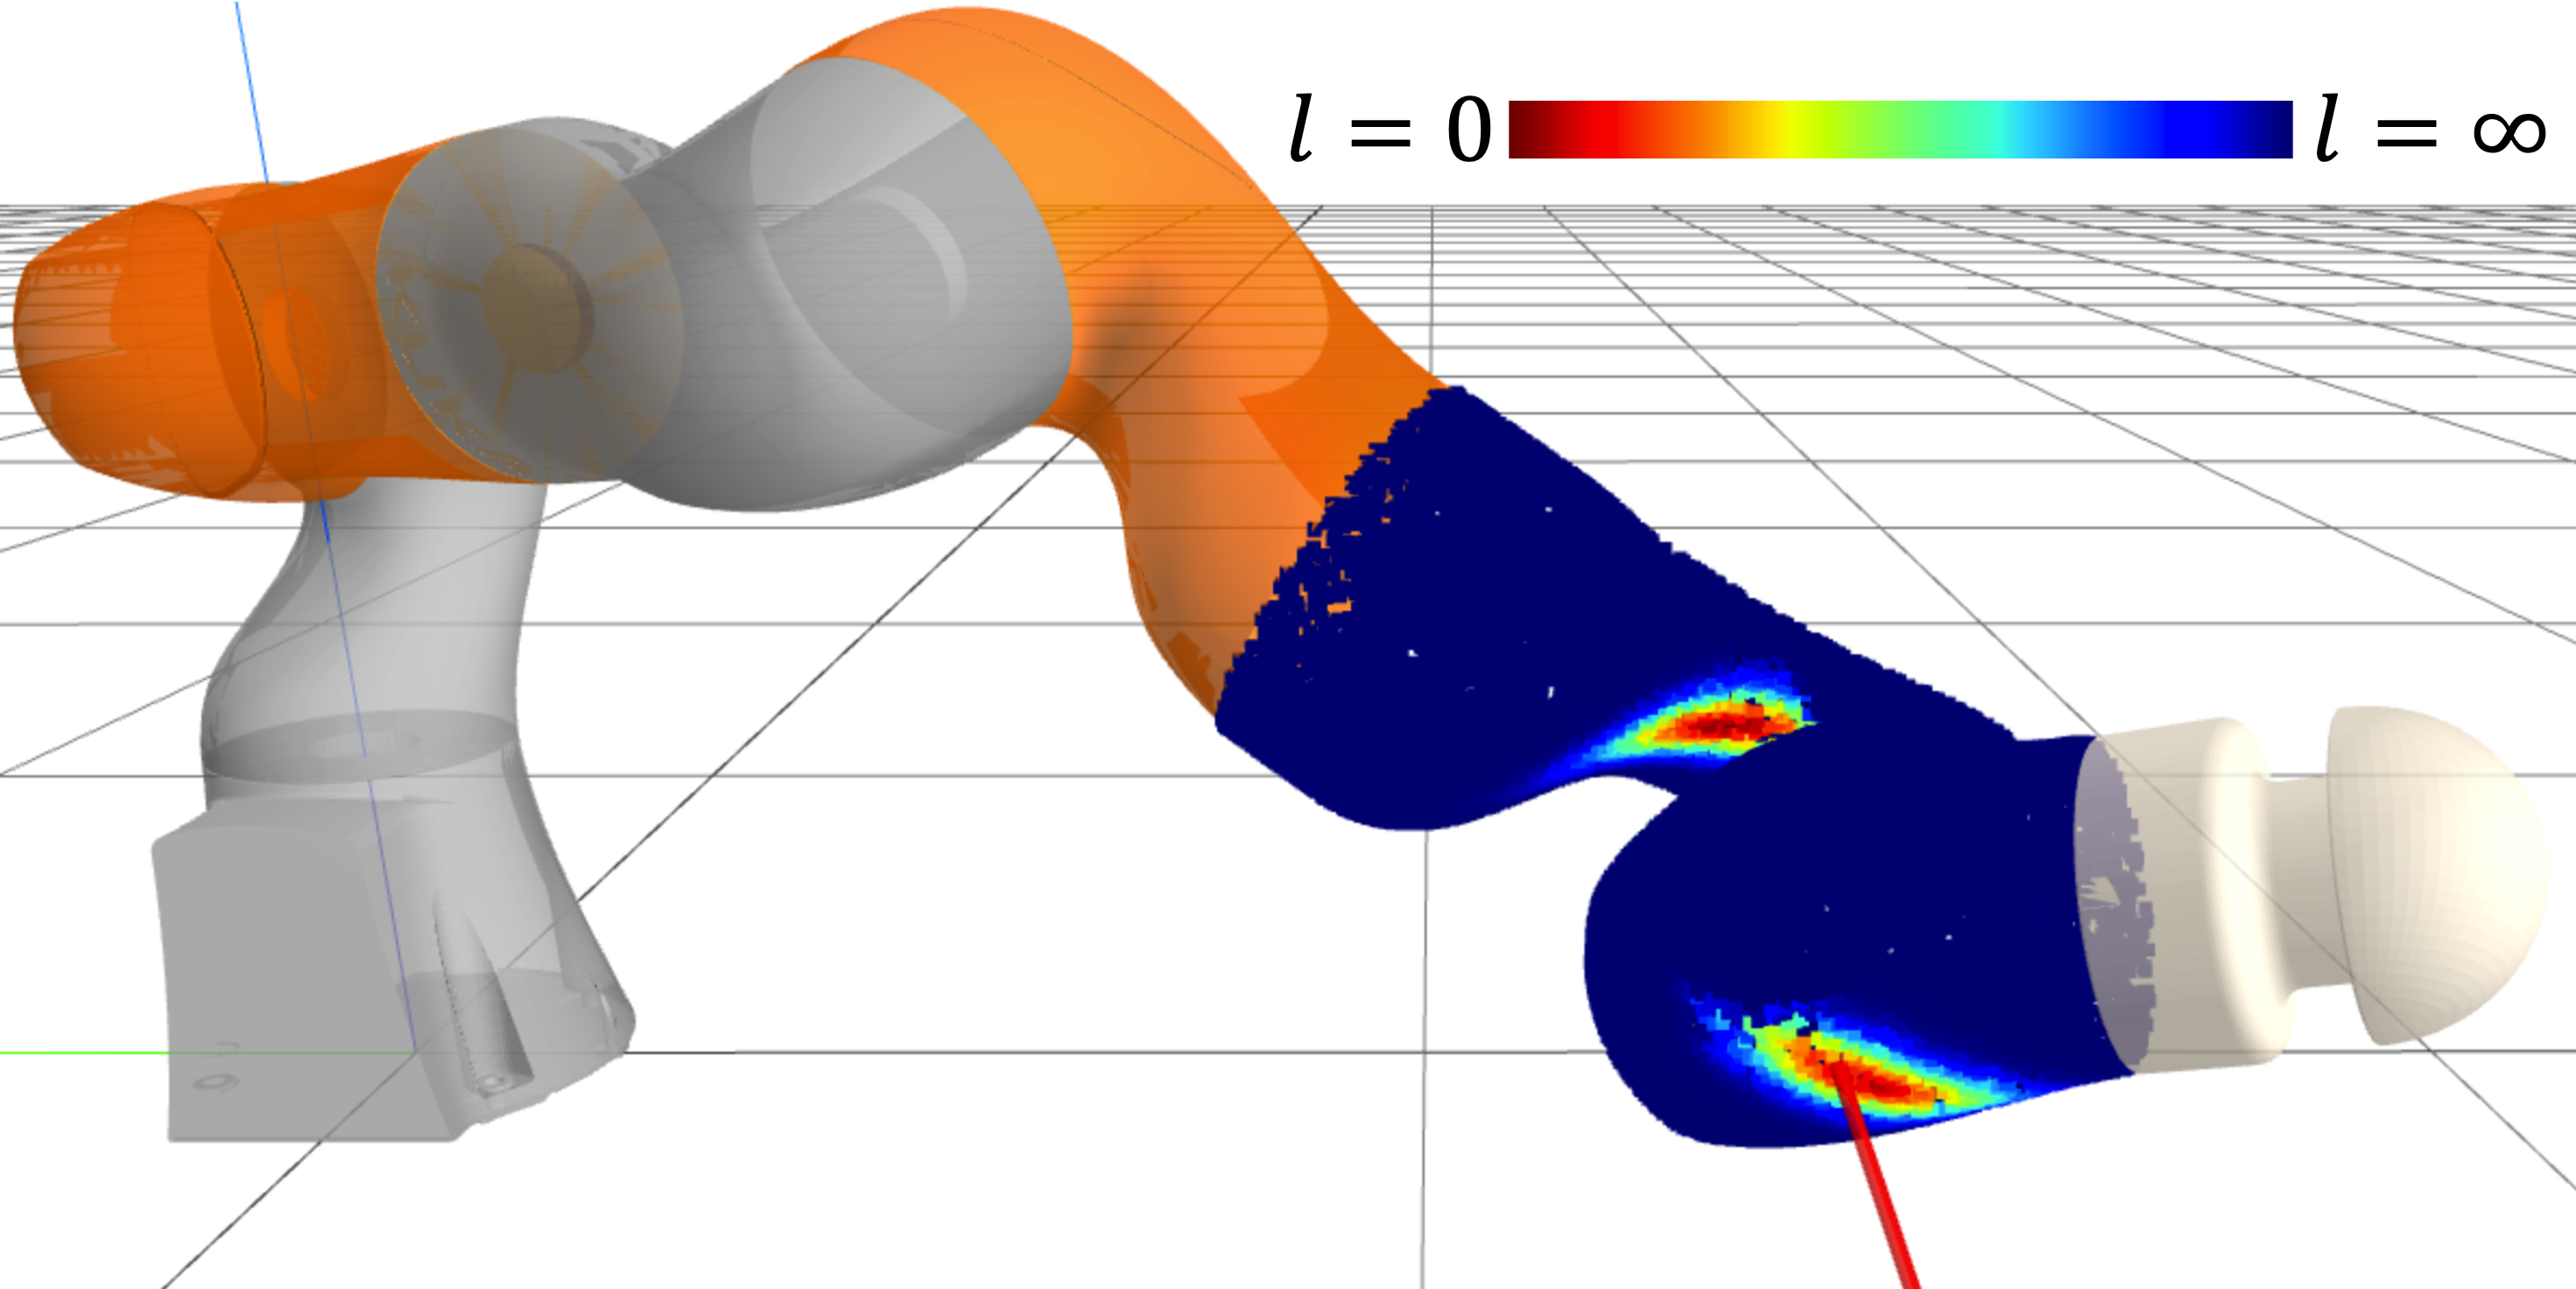
\includegraphics[width=0.85\linewidth]{figures/05_force_from_torque/multiple_local_minima.png}
\caption{The residual $l(\cdot)$ for 20000 sampled points on link 5 and 6 of the IIWA arm. The true contact position and direction is indicated by the red line. Multiple global minima of $l(\cdot)$ can be found on the robot's surface $\mathcal{S}$.}
\label{fig:multiple_local_minima}
\end{figure}

%%%%%%%%%%%%%%%%%%%%%%%%%%%%%%%%%%%%%%%%%%%%%%%%%%%%%%%%%%%%%%%%%%%%%%%%%%%%%%%%
\section{Detectability of contacts \label{sec:observability}}
The joint torque sensor of a link is only able to measure the torque about the axis of the link's revolute joint. It is therefore possible for the torque sensor to register zero or small torque measurement, even if the link is in contact with significant contact force. In this section, we give a quantitative analysis on how likely a contact force creates little or no measurable torque by studying the simplest case of a single link.

\subsection{Detectability}
We assume that a link's joint axis is aligned with the z-axis of the link's body frame. Let $\pC \in \mathcal{S}$ denote a generic point on the robot's surface, $\mathcal{K}_C$ the friction cone at $\pC$, and $\tau_z(\cdot): \mathbb{R}^3 \rightarrow \mathbb{R}$ the function that returns the z-component of the torque generated by a force. For illustrative purposes, the friction coefficient $\mu$ is set to 1. We call the contact at $\pC$ \textit{fully detectable}\footnote{The term ``detectable", which is rigorously-defined in control theory, is abused in this section in order to facilitate exposition.} if $\forall \fC \in \mathcal{K}_C$, $\norm{\fC} \neq 0 \Rightarrow \tau_z(\fC) \neq 0$. Similarly, the contact is \textit{partially detectable} if $\exists \fC \in \mathcal{K}_C$,  $\norm{\fC} \neq 0 \Rightarrow \tau_z(\fC) \neq 0$, and \textit{undetectable} if $\forall \fC \in \mathcal{K}_C$, $\tau_z(\fC) = 0$.

We first look at the condition under which a contact at $\pC$ is fully detectable. A non-zero force at $\fC$ satisfies $\tau_z(\fC) = 0$ if and only if its line of action intersects with the z-axis. The set of such $\fC$'s belong to the plane which passes through both $\pC$ and the z-axis. We denote this plane by $\mathcal{P}_C$. The contact at $\pC$ is fully detectable if and only if $\mathcal{K}_C \cap \mathcal{P}_C = \{{0}\}$, which is equivalent to the following linear program being infeasible:
\begin{subequations}
\label{eq:find_min_torque}
\begin{align}
\text{Find} \; {\beta}, \; \text{subject to} &  \\
\left(\pC \times {e}_z\right)^\intercal \left({v}_C {\beta} \right) &= 0, \label{eq:find_min_torque:plane}\\
{\beta} &\geq 1, \label{eq:find_min_torque:non-zero}
\end{align}
\end{subequations}
where ${e}_z$ is the unit vector along the z-axis; $(\pC \times {e}_z)$ is normal to $\mathcal{P}_C$. (\ref{eq:find_min_torque:plane}) constrains the contact force $\fC = {v}_C {\beta}$ to $\mathcal{P}_C$. (\ref{eq:find_min_torque:non-zero}) makes sure that $\fC$ is non-zero. 

To find out which part of a link is fully detectable, we can sample uniformly on the link's surface and solve (\ref{eq:find_min_torque}) for all samples. The results for two links with distinct geometries are shown in Fig. \ref{fig:full_observability}. As the IIWA link's surface is ``concentrated" around its joint axis, only a tiny fraction of the link's surface is fully detectable. In contrast, the ``elongated" link of UR5 has significantly more fully detectable surface, which is located further away from the joint axis. On both links, the majority of the samples are not fully detectable. 
\begin{figure}[h]
\vspace{-0.2cm}
\centering
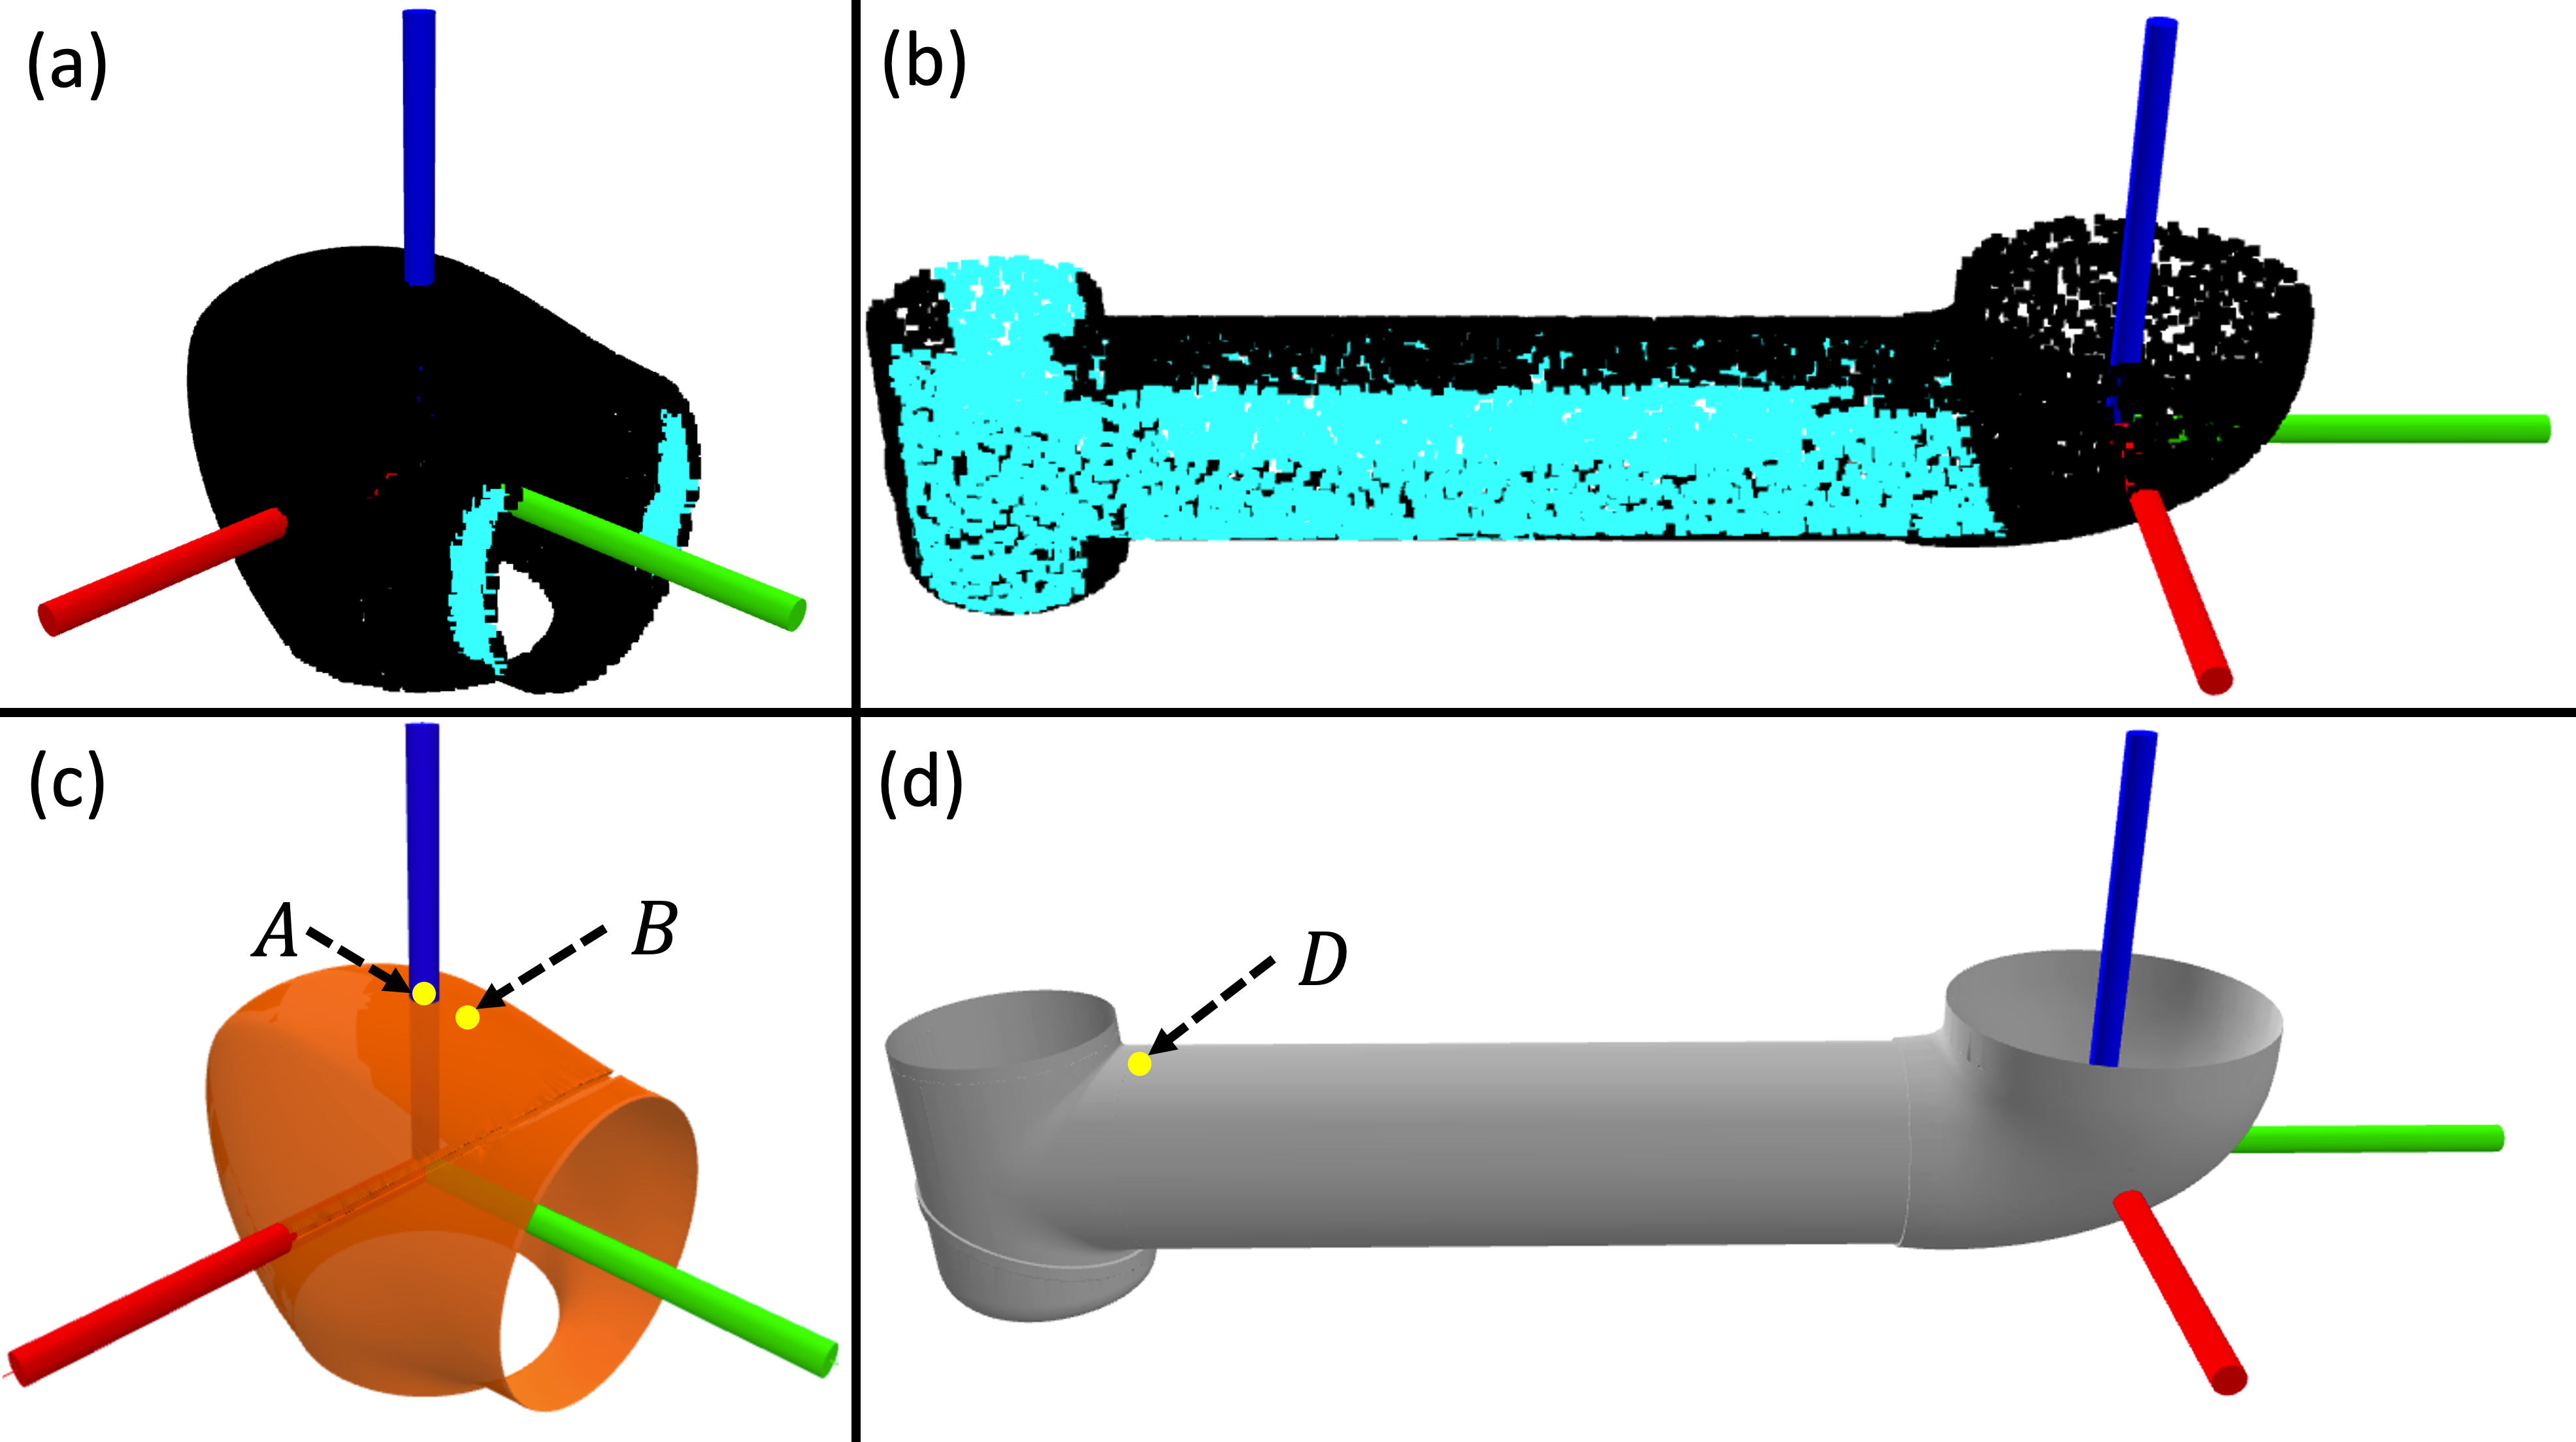
\includegraphics[width=\linewidth]{figures/05_force_from_torque/full_observability.png}
\caption{Full detectability of (\textbf{a}) link 6 of the IIWA arm and (\textbf{b}) ``forearm'' link of the UR5 arm. Out of the 20000 samples generated on each link, 2.19\% and 32.58\% of the samples on (\textbf{a}) and (\textbf{b}) are fully detectable, respectively. Fully detectable samples are shown in cyan, others in black. The meshes of the links are shown in (\textbf{c}) and (\textbf{d}).}
\label{fig:full_observability}
\vspace{-0.5cm}
\end{figure}

\subsection{Quantifying ``undetectability''}
A contact at $C$ is fully detectable if any contact force in $\mathcal{K}_C$ generates \textit{any} non-zero torque measurement. However, as real torque sensor measurements are usually corrupted by noise, it is useful to know when a contact force generates a torque measurement no less than a threshold $\epsilon$.

Moreover, for contacts that are not fully detectable, it is worth noting that the extent of their ``undetectability'' varies. For example, point $A$ in Fig. \ref{fig:full_observability}c is undetectable, as it is the intersection of the z-axis and the link's surface. Although both point $D$ (Fig. \ref{fig:full_observability}d) and $B$ (Fig. \ref{fig:full_observability}c) are partially detectable, it generally takes a smaller force to generate $\tau_z > \epsilon$ at $D$ than at $B$, as $D$ is further away from its joint axis.

The degree of a contact's ``undetectability'' with respect to the threshold $\epsilon$ can be quantified by:
\begin{subequations}
\begin{align}
\eta_\epsilon(\pC) &\coloneqq \frac{\text{Area}(\mathcal{D}_c^\epsilon)}{\text{Area}(\mathcal{D}_c)} \in [0, 1],  \\
\mathcal{D}_C &\coloneqq \{\fC \in \mathbb{R}^2 : \norm{\fC} = 1, \fC \in \mathcal{K}_C\}, \\
\mathcal{D}_C^\epsilon &\coloneqq \{\fC \in \mathcal{D}_C : \tau_z(\fC) \leq \epsilon \}, 
\end{align}
\end{subequations}
where $\mathcal{D}_C$ is a ``dome" in the friction cone consisting of unit-norm forces, and $\mathcal{D}_C^\epsilon$ is the subset of $\mathcal{D}_C$ consisting of forces whose torque measurement $\tau_z(\fC)$ is less than $\epsilon$. Intuitively, $\eta_\epsilon(\pC)$ is the proportion of contact forces in $\mathcal{K}_C$ that create small ($\leq \epsilon$) torque measurements. The closer $\eta(\pC)$ is to 1, the less detectable $\pC$ becomes. Using Fig. \ref{fig:full_observability}c and \ref{fig:full_observability}d again as examples, we expect $\eta_\epsilon({p}_A) = 1$, $\eta_\epsilon({p}_B)$ be close to 1, and $\eta_\epsilon({p}_D) < \eta_\epsilon({p}_B)$. 

Computing $\eta_\epsilon(\pC)$ can be done analytically, but a sampling based approach is much easier to implement. Uniform samples on $\mathcal{D}_C$ can be easily generated, and checking membership of $\mathcal{D}_C^\epsilon$ is trivial. We can then approximate $\eta_\epsilon(\pC)$ by the ratio of samples in $\mathcal{D}_C^\epsilon$ to the total number of samples.

To evaluate the ``undetectability" of an entire link, we can once again compute $\eta_\epsilon(\cdot)$ for samples generated uniformly from the link's surface. The results for two different links using different $\epsilon$'s are summarized in Fig. \ref{fig:partial_observability}. As $\epsilon$ increases, the surface close to the z-axis quickly becomes fully undetectable. If we treat $\epsilon$ as a detection threshold, the result becomes particularly alarming for links with a more ``concentrated" shape: even for $\epsilon=0.02$ (Fig. \ref{fig:partial_observability_eisilon_0.02}): $\eta_\epsilon \geq 0.4$ for 80\% of the samples. In other words, if a force of $1\mathrm{N}$ is applied at a random point $C$ along a random direction in $\mathcal{K}_C$, the probability of not detecting the contact force is at least 0.32.

\begin{figure}
\centering
\subfloat[$\epsilon$=0.02. IIWA: $\eta_{\text{min}}=0.011, \eta_{\text{max}}=1$. UR5: $\eta_{\text{min}}=0, \eta_{\text{max}}=1$.]{
	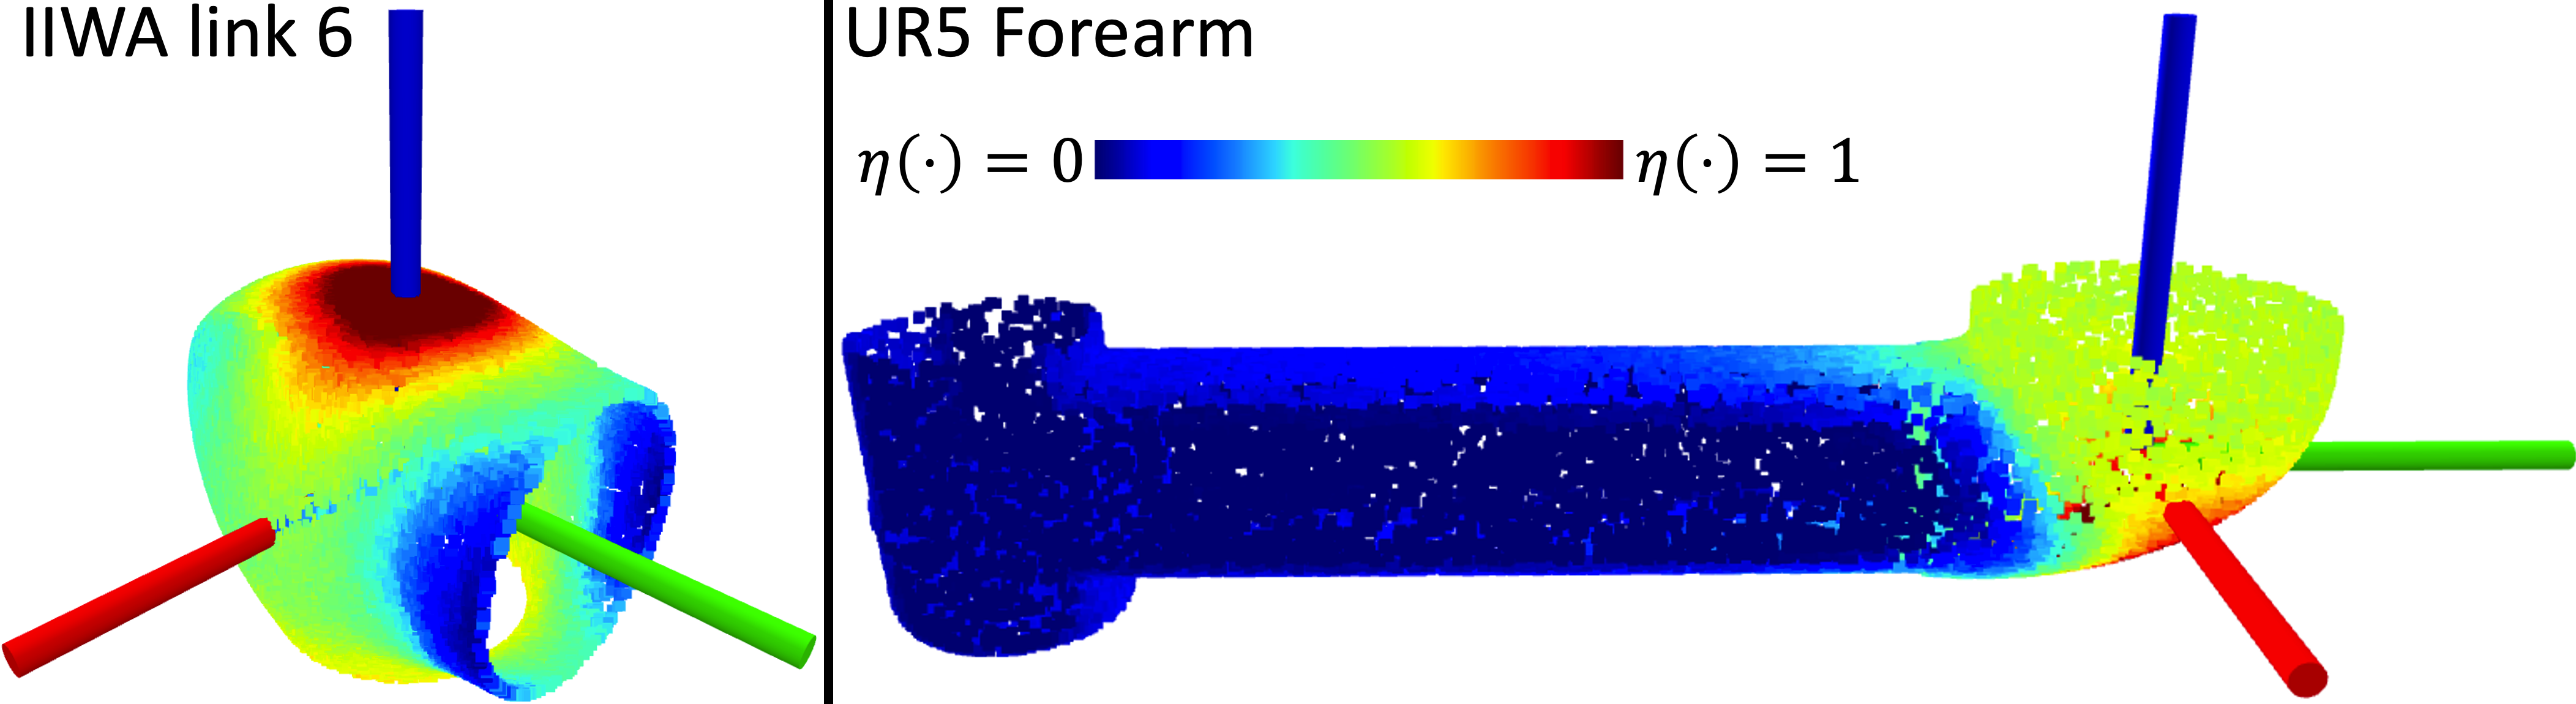
\includegraphics[width=0.97\linewidth]{figures/05_force_from_torque/partial_observability_eisilon_0.02.png}
	\label{fig:partial_observability_eisilon_0.02}
}\\
\subfloat[$\epsilon$=0.05. IIWA: $\eta_{\text{min}}=0.249, \eta_{\text{max}}=1$. UR5: $\eta_{\text{min}}=0, \eta_{\text{max}}=1$.]{
	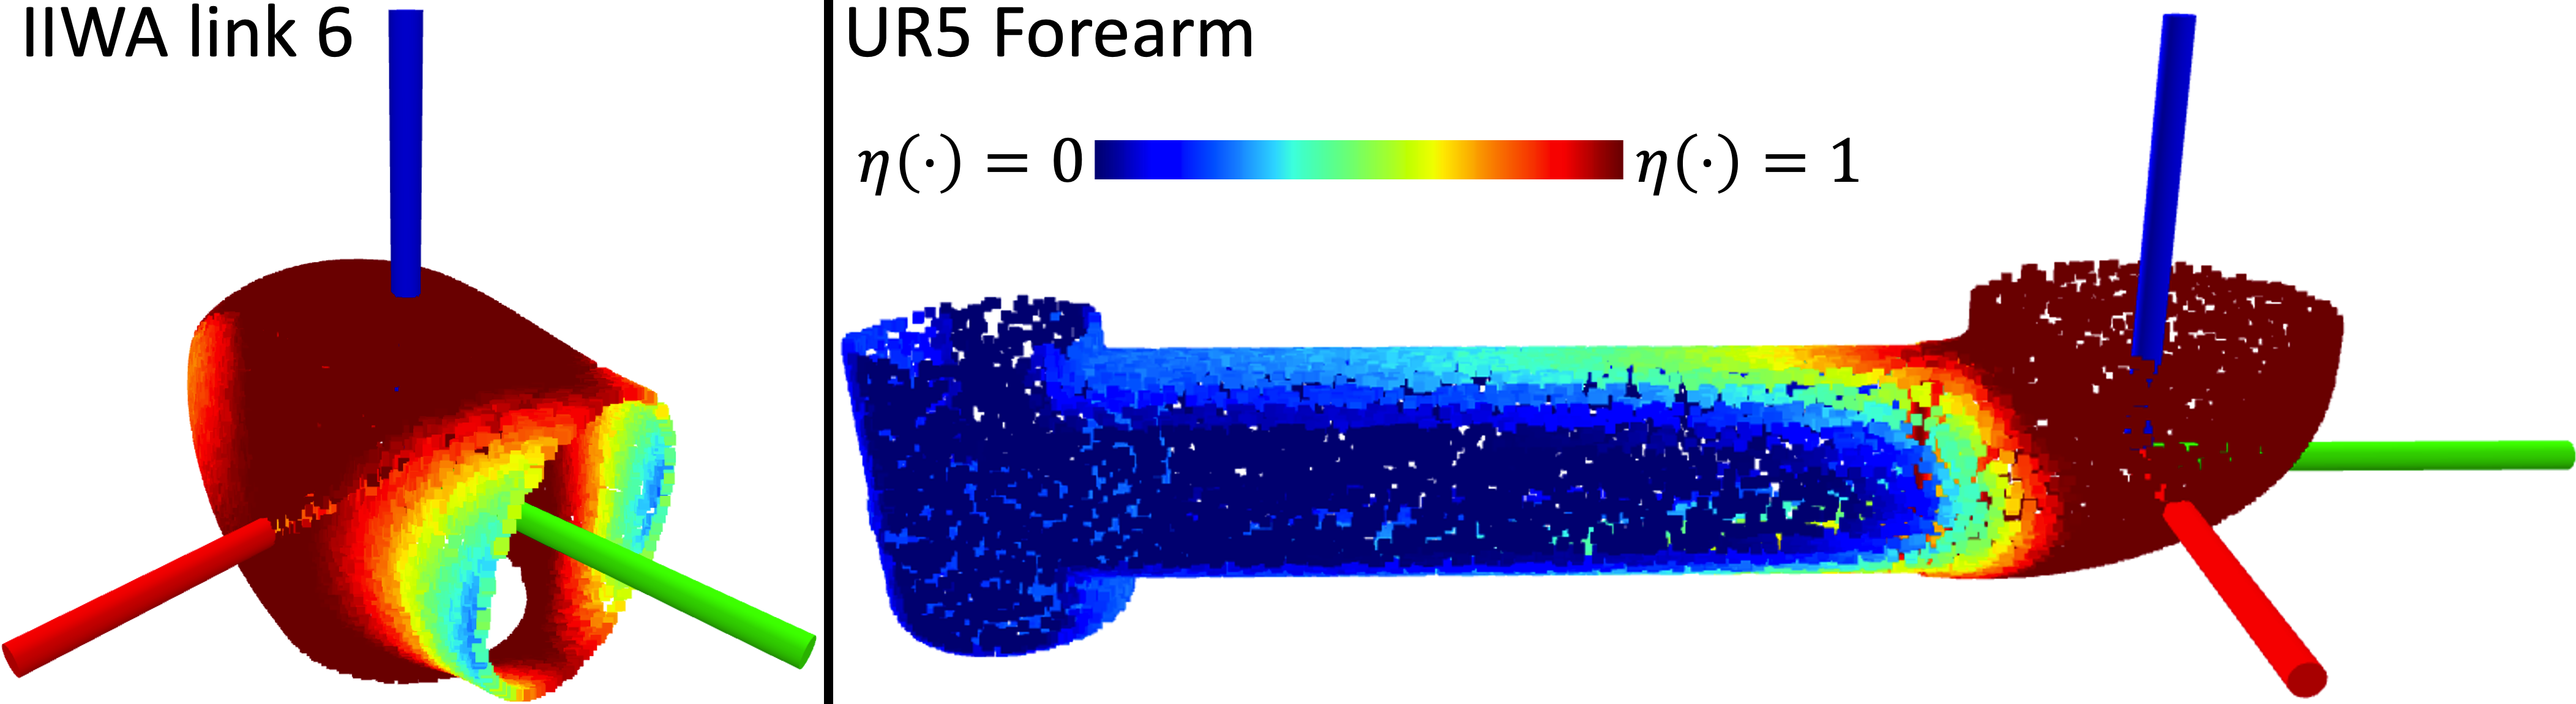
\includegraphics[width=0.97\linewidth]{figures/05_force_from_torque/partial_observability_eisilon_0.05.png}
	\label{fig:partial_observability_eisilon_0.05}
}\\
\subfloat[$\epsilon$=0.1. IIWA: $\eta_{\text{min}}=1, \eta_{\text{max}}=1$. UR5: $\eta_{\text{min}}=0, \eta_{\text{max}}=1$.]{
	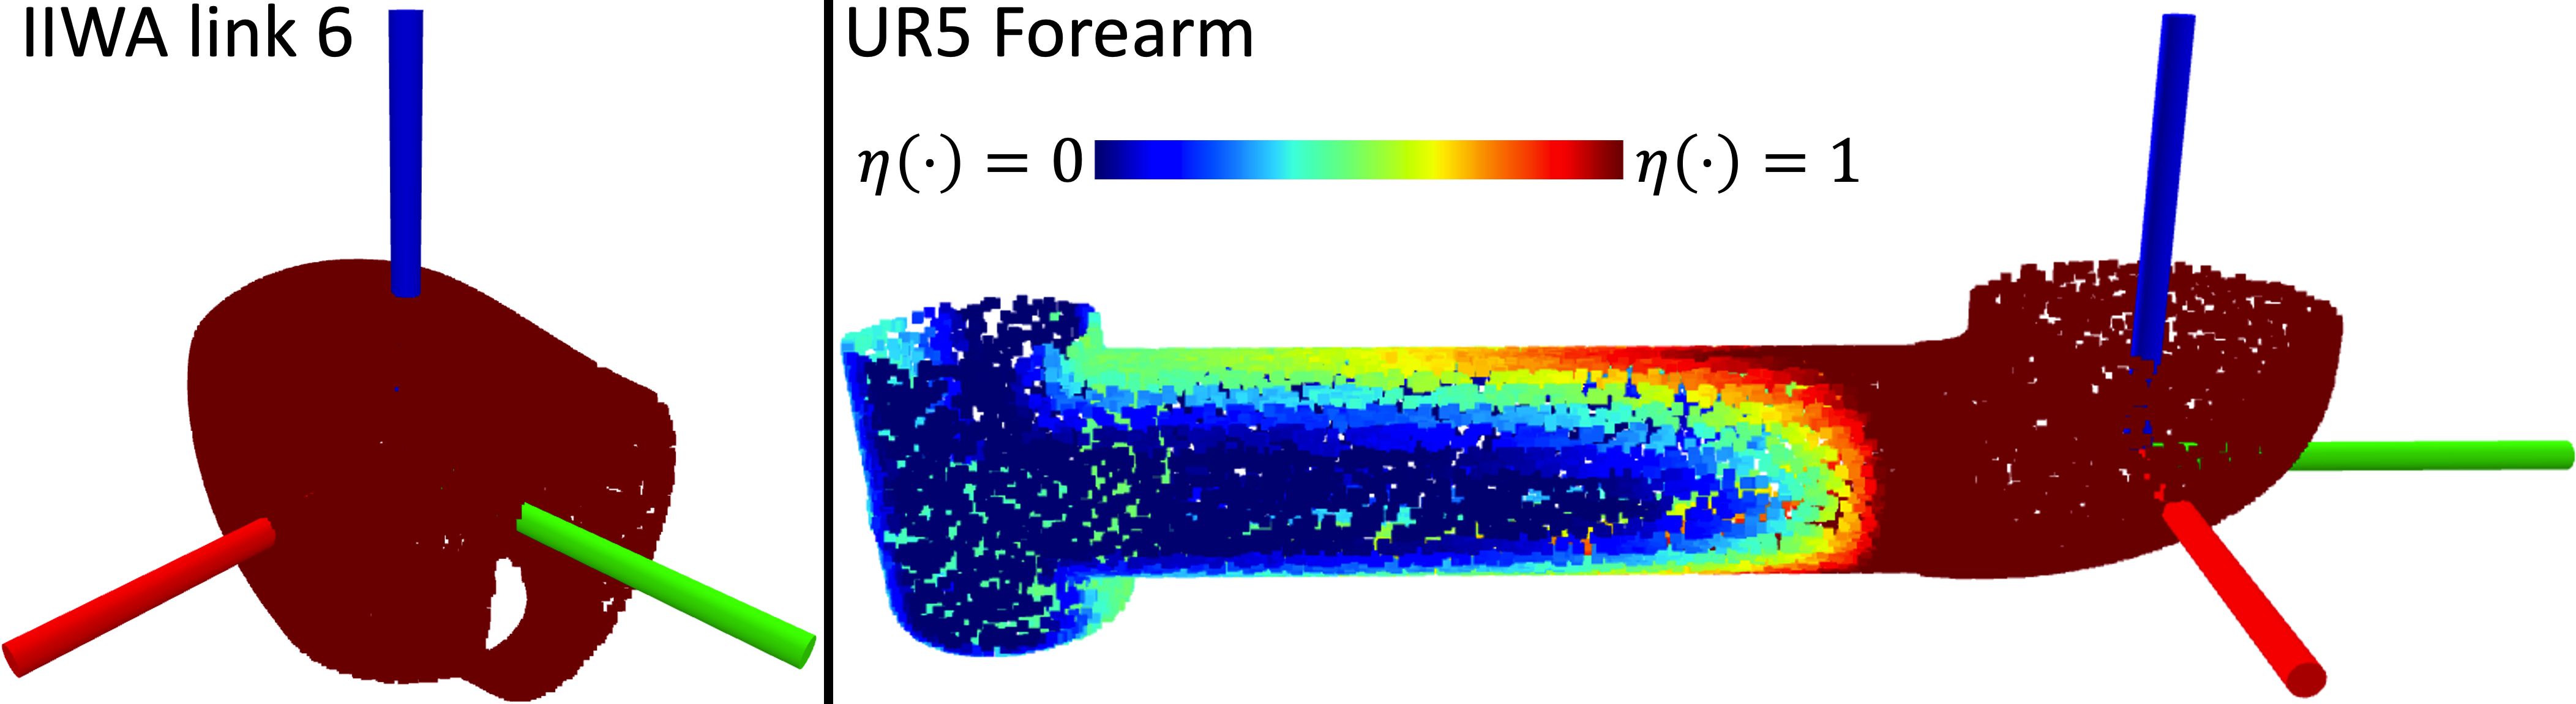
\includegraphics[width=0.97\linewidth]{figures/05_force_from_torque/partial_observability_eisilon_0.1.png}
	\label{fig:partial_observability_eisilon_0.1}
}
\caption{$\eta_\epsilon(\cdot)$ of IIWA link 6 and UR5 forearm. }
\label{fig:partial_observability}
\end{figure}

\subsection{Implications}
The analysis in this section reveals a fundamental limitation of existing joint-torque-based contact estimation methods: when a contact force generates small torque about the axis of a link, the observed $\tauE$ could be equally well explained by a different contact point on a different link.

Haddadin's method \cite{haddadin2017robot} determines the link in contact as the most distal link with $\tau_z(\cdot) \geq \epsilon$. As there is a significant chance that $\tau_z(\pC) \leq \epsilon$ at the true contact position $C$, it is likely that their strategy believes the contact to be on a wrong link. MCMC methods \cite{manuelli2016localizing, zwiener2019armcl} evaluate the likelihood of points being the true contact point $C$ using the residual (\ref{eq:residual_qp}). If $\eta_\epsilon(\pC)$ is large, it is likely for other points to have a residual that is only larger by $\epsilon^2 \norm{\fC}^2$, thereby trapping MCMC methods in a wrong local minimum of $l(\cdot)$. 

%%%%%%%%%%%%%%%%%%%%%%%%%%%%%%%%%%%%%%%%%%%%%%%%%%%%%%%%%%%%%%%%%%%%%%%%%%%%%%%%
\section{Contact estimation from external torque measurements}
We have demonstrated that the best contact estimate achievable from $q$ and $\tauE$ is $P_0(q, \tauE)$ (Section \ref{sec:problem_statement}), which is likely to have more than one element (Section \ref{sec:observability}). Elements of $P_0(q, \tauE)$ are global optimizers of (\ref{eq:nonlinear_program}), which are also global minima of the residual $l(\cdot; q, \tauE)$ on $\mathcal{S}$. However, due to the dependence of ${J}$ on $\pCbar$ and the manifold constraint $\pCbar \in \mathcal{S}$, (\ref{eq:nonlinear_program}) is nonlinear and difficult to solve directly.

In this section, we present a contact estimation strategy called RSGD, which is named after the combination of Rejection Sampling and Gradient Descent. RSGD is able to find every local minima of $l(\cdot; q, \tauE)$. Although not as ideal as finding $P_{0}(q, \tauE)$, RSGD is stronger than MCMC methods: it locates every point on $\mathcal{S}$ to which MCMC methods may converge.

\subsection{Rejection sampling}
Starting with $P \coloneqq \{\pCbar \in \mathcal{S} \}$, a set of uniform samples drawn from $\mathcal{S}$, we can calculate the residual $l(\cdot)$ for all samples in $P$, and keep the samples which satisfy $ l \leq \epsilon$:
\begin{equation}
P_{\epsilon}(q, \tauE) \coloneqq \{\pCbar \in \mathcal{S} : l(\pCbar; q, \tauE) \leq \epsilon\}. 
\end{equation}

When using a dense $P$ (Fig. \ref{fig:rejection_sampling}a), $|P_{\epsilon}|$ is usually sufficiently large so that the local minima of $l(\cdot)$ can be estimated, for instance, by clustering the points in $P_{\epsilon}$, finding the cluster centers, and then projecting the centers back onto the robot surface $\mathcal{S}$. In contrast, when $P$ is sparse (Fig. \ref{fig:rejection_sampling}b), the few samples in $P_{\epsilon}$ are typically too noisy to make a reasonable estimate. 

The biggest drawback of rejection sampling is the high rejection rate, which, for example, can get to approximately 98\% for the robot and contact configuration in Fig. \ref{fig:rejection_sampling}. Calculating residuals for a very dense $P$ is therefore needed for an accurate contact estimate, which will incur prohibitively high computational cost.
\begin{figure}[h]
    \centering
    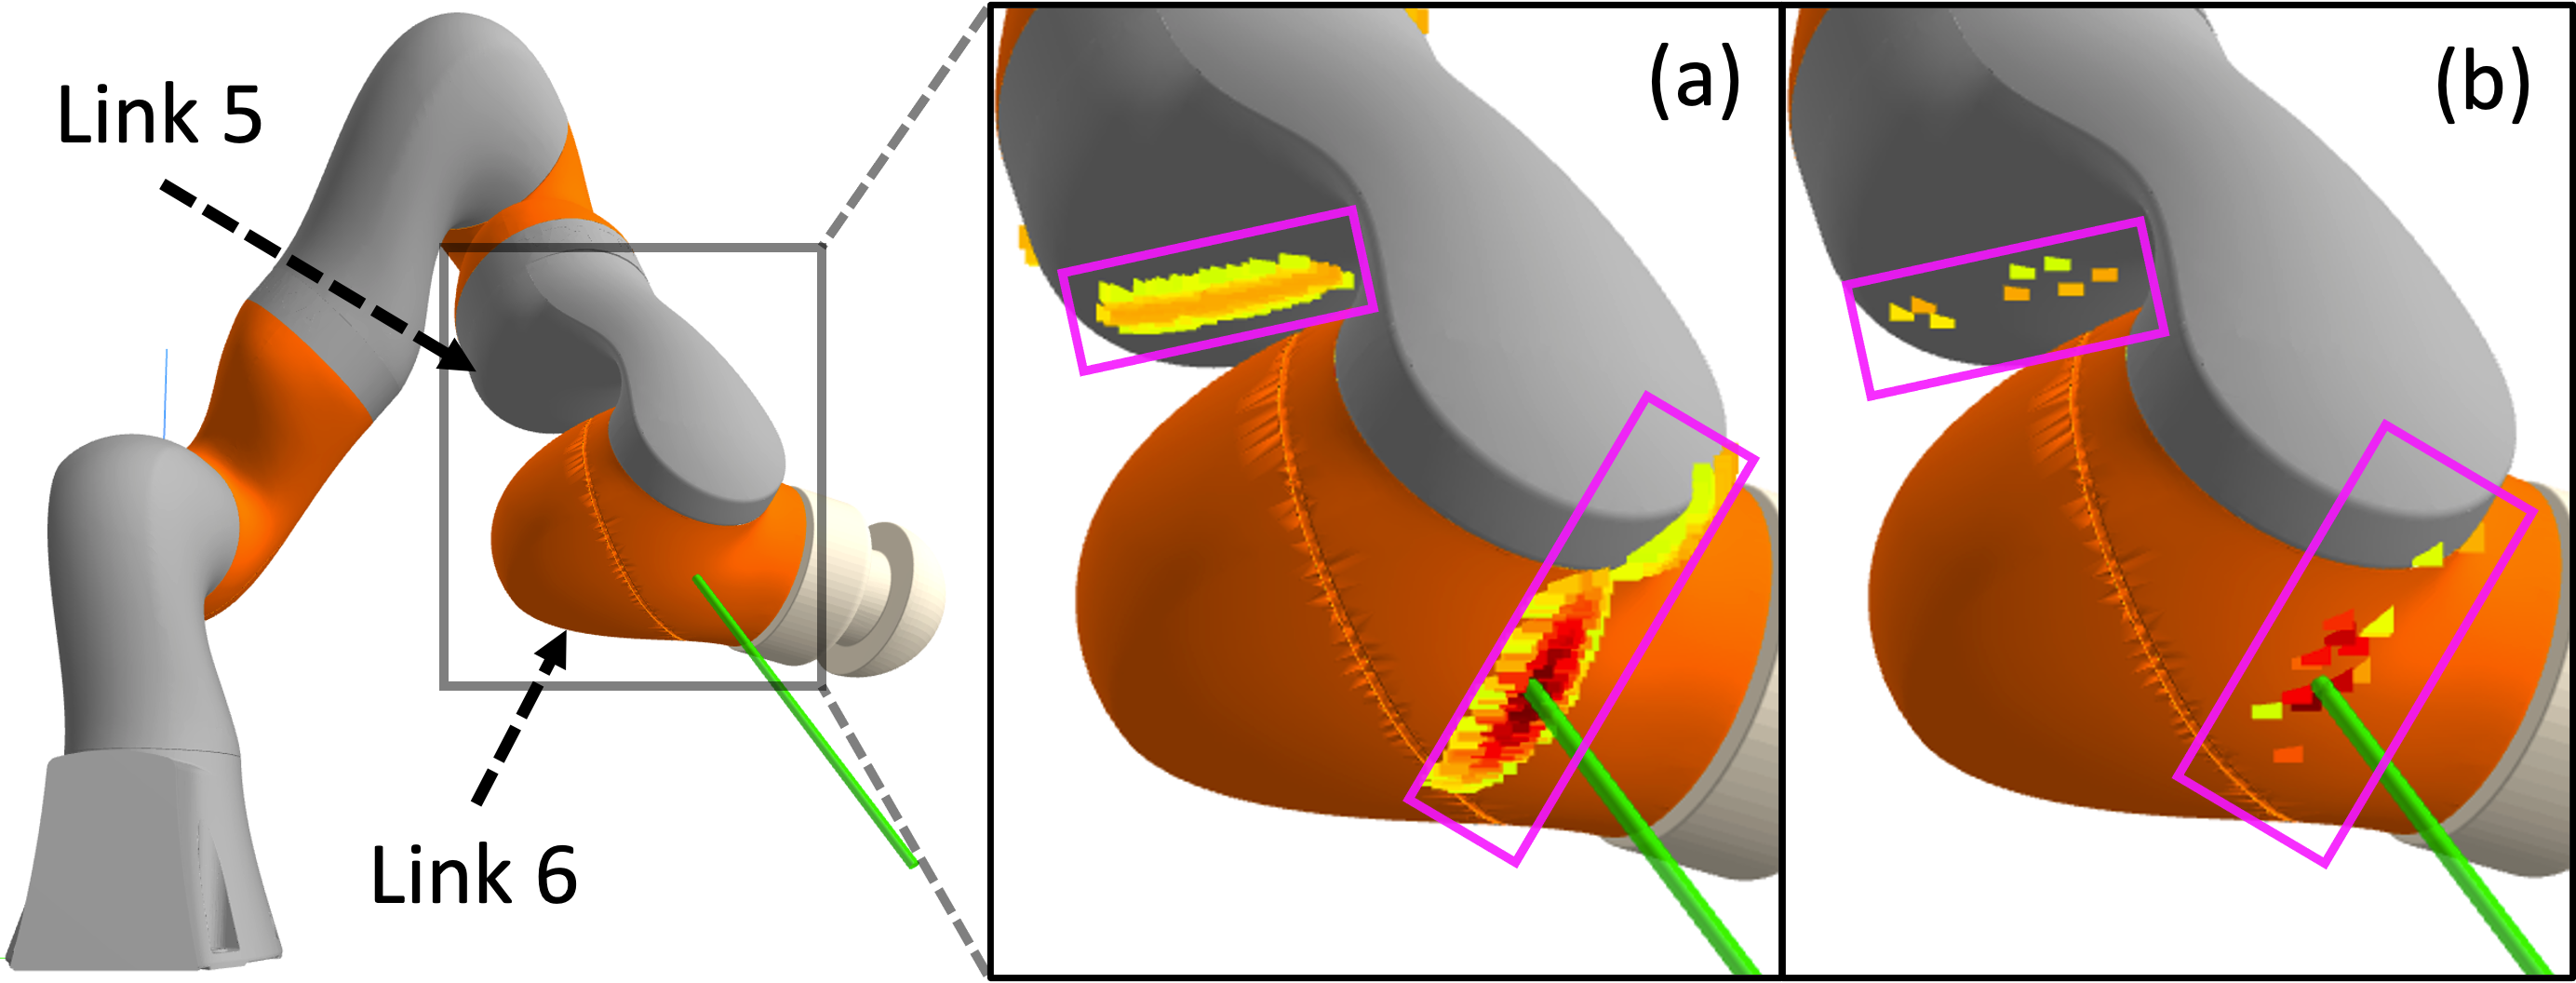
\includegraphics[width=\linewidth]{figures/05_force_from_torque/rejection_sampling.png}
    \caption{Finding elements of $P_{\epsilon}$ on link 5 and link 6 with $\epsilon=0.005$ using rejection sampling. A force of $10\mathrm{N}$ is applied to the robot along the green line. Enclosed by magenta boxes, the colored squares represent accepted samples. (\textbf{a}) Dense $P$: 491 out of 20000 samples are accepted.  (\textbf{b}) Sparse $P$: 24 out of 1000 samples are accepted.}
    \label{fig:rejection_sampling}
    \vspace{-0.6cm}
\end{figure}

\subsection{Rejection sampling + gradient descent (RSGD)\label{sec:proposed_contact_estimator}}
The high computational cost of vanilla rejection sampling, due to the high rejection rate for small $\epsilon$, can be reduced significantly by
\begin{enumerate}
\item  Generating a set of potential contact positions by rejection sampling using a sparse sample set $P$ and a large threshold $\delta$: $P_{\delta}(q, \tauE) \coloneqq \{\pCbar \in \mathcal{S} : l(\pCbar; q, \tauE) \leq \delta\}$.

\item  Running gradient descent (Algorithm \ref{algo:gradient_descent}) for every $\pCbar \in P_{\delta}(q, \tauE)$, collecting the converged points $\pCbar^*$ into a set of locally optimal contact position estimates: $P^\star_{\delta}(q, \tauE) \coloneqq \{\pCbar^* \in \mathcal{S}\}.$
\end{enumerate}

As shown in Fig. \ref{fig:rsgd}, a large $\delta$ in Step 1 increases the acceptance rate, ensuring that $P_{\delta}$ has enough samples even if the initial sample set $P$ is sparse. Although samples in $P_{\delta}$ are spread out at the beginning, Step 2 runs them through Algorithm 1, making most of them converge to local minima of $l(\cdot)$.
\begin{algorithm}[h]
\caption{Gradient descent on manifold $\mathcal{S}$}\label{algo:gradient_descent}
\textbf{Input}: ${q}$, $\tauE$, $\pCbar$\; 
\textbf{Output}: $\pCbar^*$\;
\While{$\norm{\nabla_{\pCbar} l(\pCbar; q, \tauE)} > \varepsilon_G$} {
    ${t} \gets \left({I}_3 - {n}_C {n}_C^\intercal \right)\nabla_{\pCbar} l(\pCbar; q, \tauE)$ \label{algo:gradient_descent:gradient_projection}\;
    $a \gets \mathrm{LineSearch}(\pCbar, {t})$ \label{algo:gradient_descent:line_search}\;
    $\pCbar \gets \pCbar + a {t}$\;
    $\pCbar \gets \mathrm{Retract}(\pCbar, \mathcal{S})$ \label{algo:gradient_descent:retract}\;
}

$\pCbar^* \gets \pCbar$\;
\end{algorithm}

\begin{figure}[h]
\centering
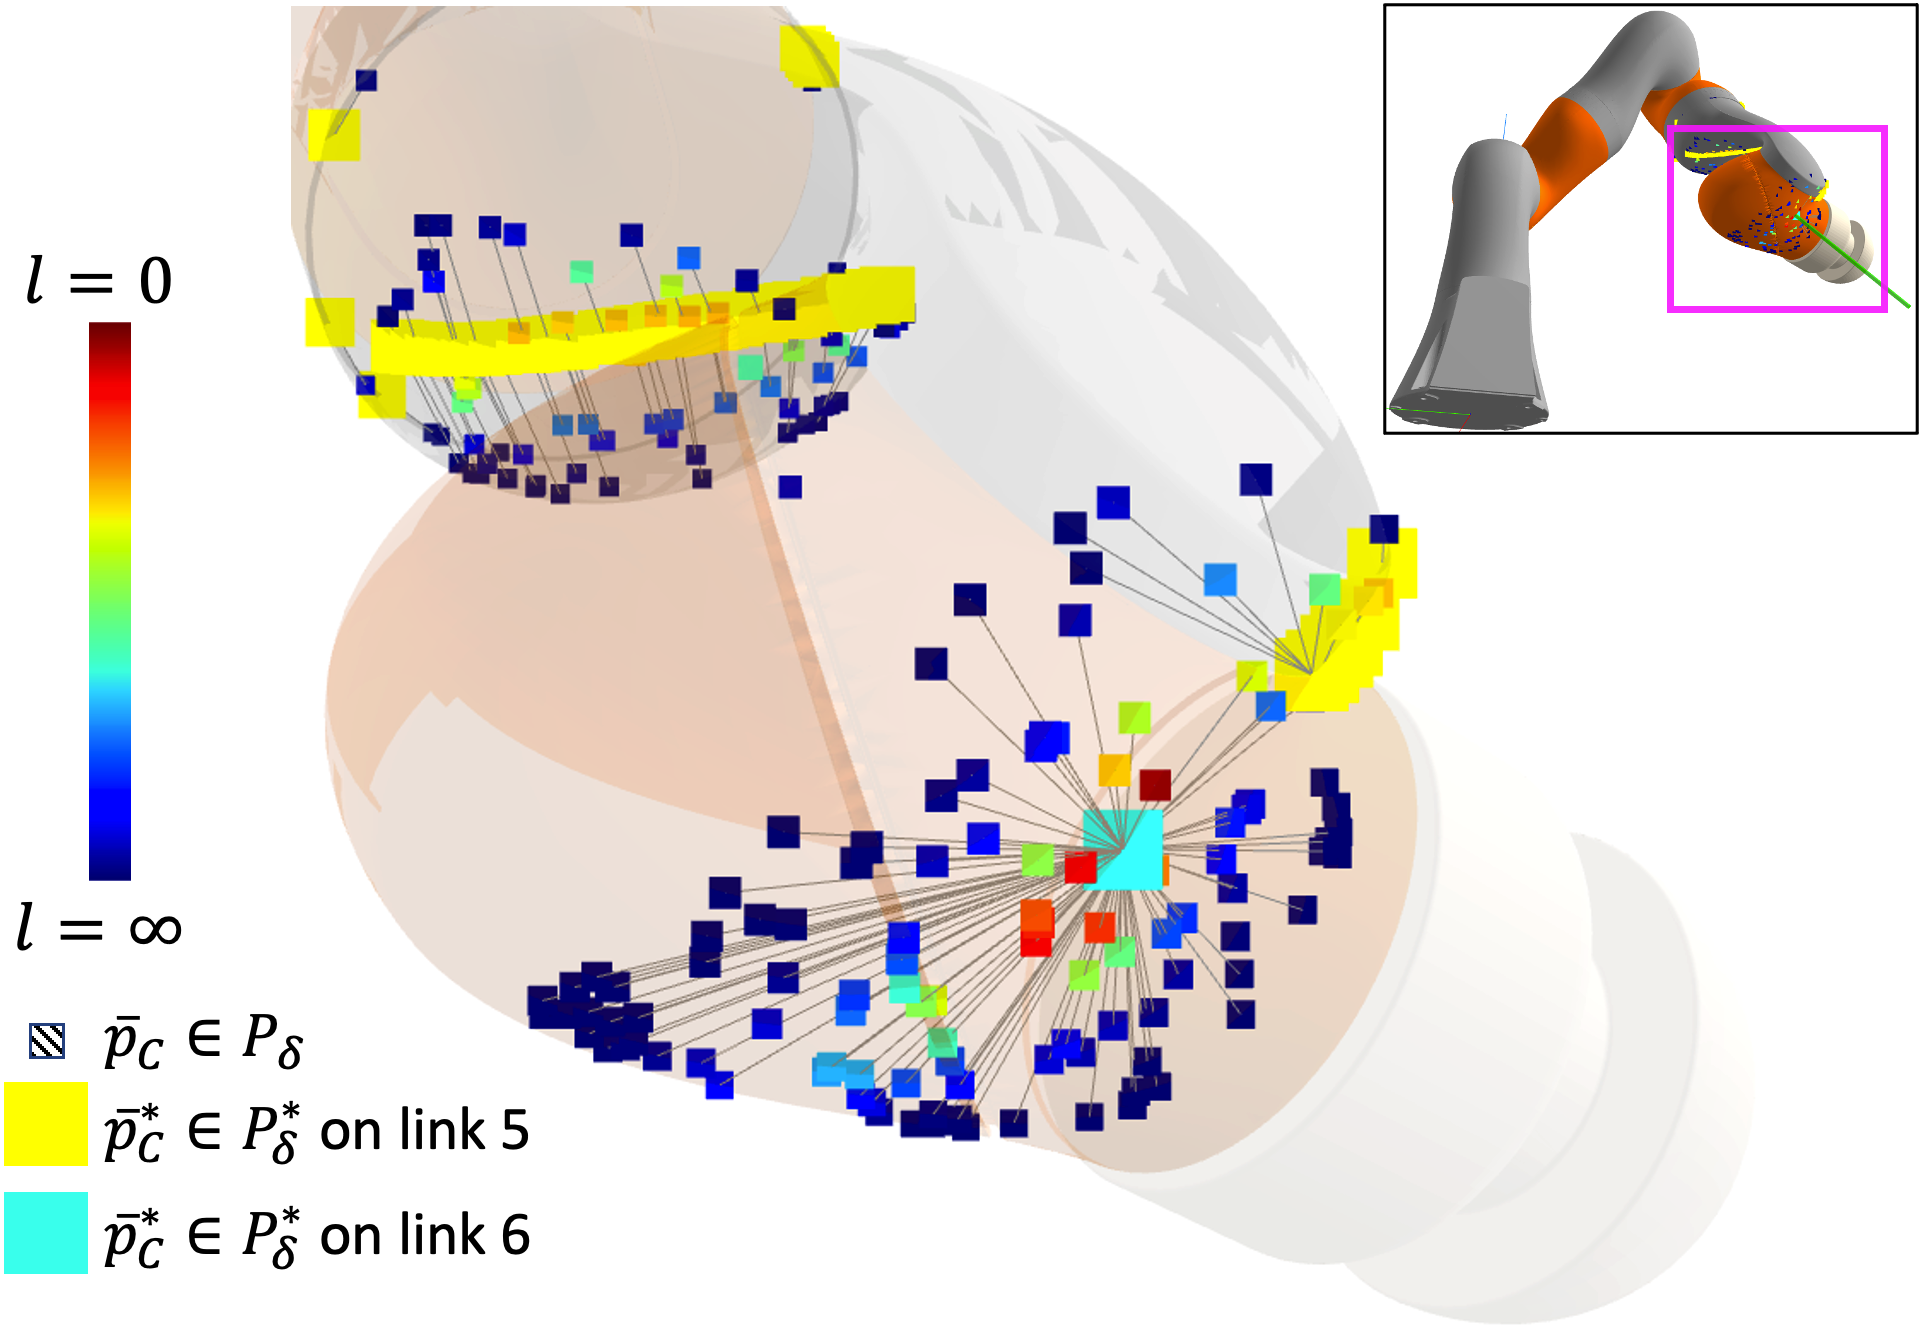
\includegraphics[width=0.9\linewidth]{figures/05_force_from_torque/rsgd.png}
\caption{Running RSGD on the same robot and contact configuration as Fig. \ref{fig:rejection_sampling}. Step 1: 175 out of 1000 samples are accepted with $\delta = 0.1$, which are shown as small squares color-coded by their residual values $l$. Step 2: 155 of the 175 samples in $P_\delta$ converge after running Algorithm 1, which are shown as large squares. Every $\pCbar \in P_\delta$ is connected by a line to the corresponding element in $P_\delta^*$ to which it converges.}
\label{fig:rsgd}
\end{figure}

Algorithm \ref{algo:gradient_descent} is the standard Gauss-Newton method for Riemannian optimization. In Line \ref{algo:gradient_descent:gradient_projection}, the gradient $\nabla_{\pCbar} l$ is projected to the local tangent plane, which has normal ${n}_C$ and passes through $\pCbar$. In Line \ref{algo:gradient_descent:line_search}, a standard line search method is used to ensure that $l$ is decreasing after taking the gradient step $a{t}$ \cite{boyd2004convex}. In Line $\ref{algo:gradient_descent:retract}$, the new point in the local tangent plane is projected back onto $\mathcal{S}$.

Using (\ref{eq:residual_qp:qp}), the gradient $\nabla_{\pCbar} l$ can be written as 
\begin{equation}
\label{eq:l_gradient_chain_rule}
\left(\nabla_{\pCbar} l \right)^\intercal =
\frac{\partial l}{\partial \pCbar} = \frac{\partial l}{\partial \mathbf{Q}} \frac{\partial \mathbf{Q}}{\partial \pCbar} + \frac{\partial l}{\partial {b}} \frac{\partial {b}}{\partial \pCbar}
\end{equation}
where $\frac{\partial \mathbf{Q}}{\partial \pCbar}$ and $\frac{\partial {b}}{\partial \pCbar}$ can be obtained using automatic differentiation \cite{griewank1989automatic}$; \frac{\partial l}{\partial \mathbf{Q}}$ and $\frac{\partial l}{\partial {b}}$ can be obtained from differentiating the implicit function defined by the optimality condition of QP (\ref{eq:residual_qp:qp}) \cite{boot1963sensitivity}.

As shown in Fig. \ref{fig:gradient_descent}a, Algorithm 1 is effective at reducing the residual $l(\cdot)$ of samples in $P_\delta$. Note that about 60 samples converge to positions on $\mathcal{S}$ with $l = 0.003$, which is a local minimum on link 5, but not the global minimum on link 6. An example gradient descent run is shown in Fig. \ref{fig:gradient_descent}b.
\begin{figure}[h]
\centering
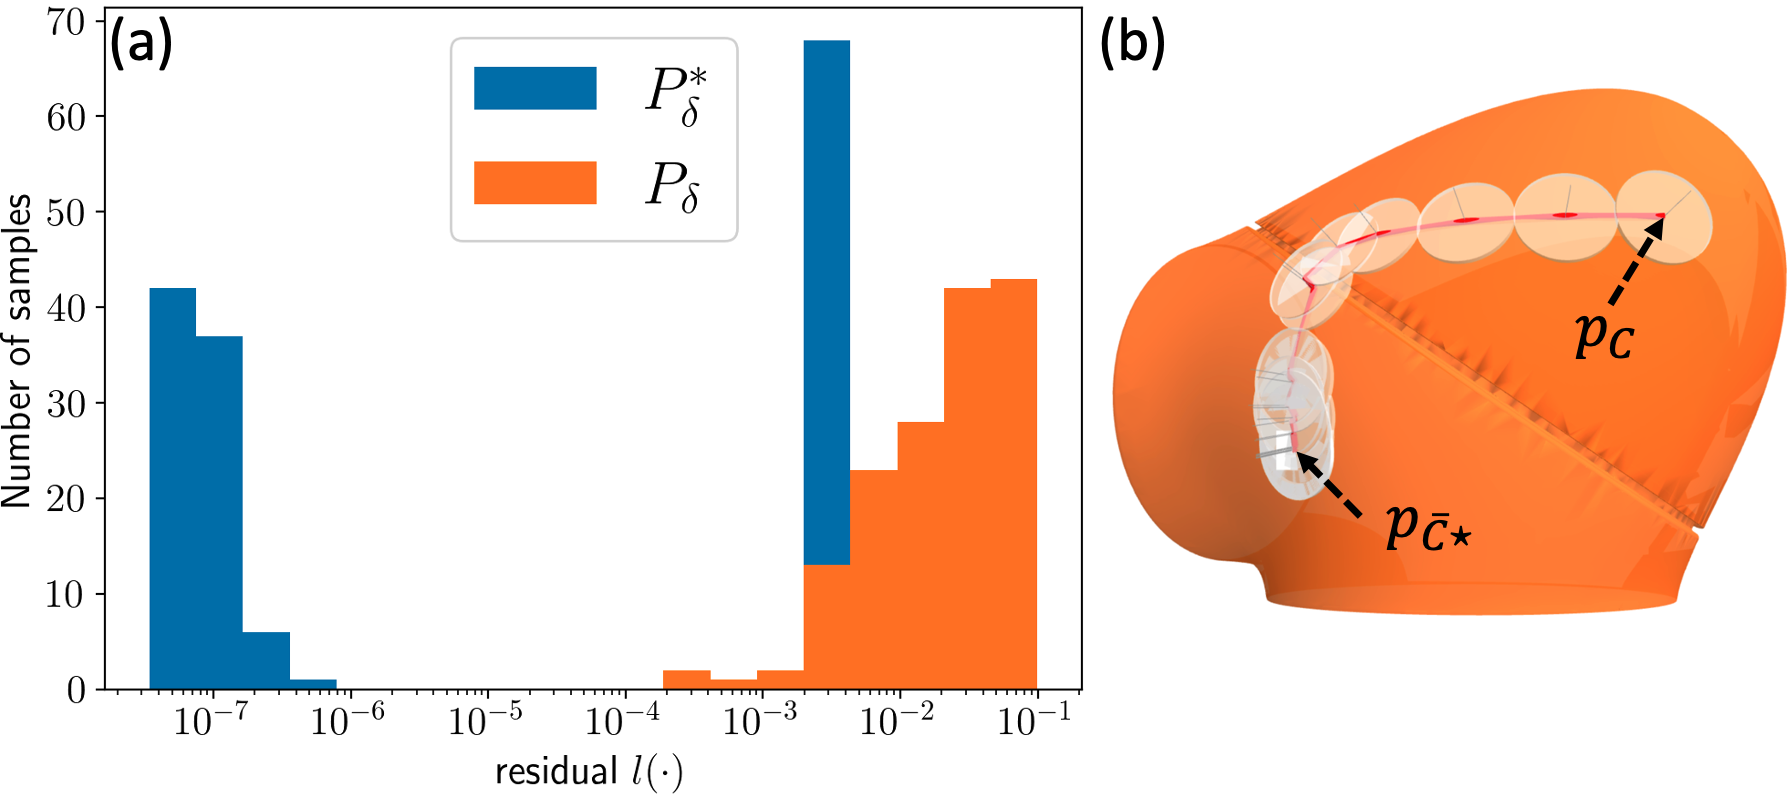
\includegraphics[width=0.85\linewidth]{figures/05_force_from_torque/gradient_descent.png}
\caption{(\textbf{a}) Distribution of residual $l(\cdot)$ of the $P_\delta$ and $P_\delta^*$ from Fig. \ref{fig:rsgd}. (\textbf{b}) A gradient descent run on link 6 of IIWA. Algorithm \ref{algo:gradient_descent} starts at $\pCbar \in \mathcal{S}$ and converges to $\pCbar^*$. Red lines represent the path taken by gradient descent. White translucent disks represent local tangent planes. }
\label{fig:gradient_descent}
\vspace{-1.0cm}
\end{figure}

The ability of an approach such as RSGD to find all local minima depends on two factors: the sampling strategy and the convergence properties of gradient descent. 
% Concerning the former, 
By construction the entire surface of the robot is contained with the support of the distribution of the sampling procedure.
As such, for every local minimum that has a non-measure-zero region of attraction, the probability that we draw a sample in that region and converge to the minimum in non-zero.  
Characterizing these regions of attraction, however, is more challenging, and one cannot rule out, e.g. saddle points and limit cycles. 
Nevertheless, empirically, we observe that the algorithm succeeds in finding all local minima for sufficiently dense sampling.

%%%%%%%%%%%%%%%%%%%%%%%%%%%%%%%%%%%%%%%%%%%%%%%%%%%%%%%%%%%%%%%%%%%%%%%%%%%%%%%%
\section{Active contact discrimination}
In the event that RSGD returns multiple (possible) contacts, some form of active exploration may be desirable to discriminate the true contact from the spurious.
Assuming contact with a static object, that will remain (approximately) in place irrespective of the robot's motion, a simple strategy to falsify a spurious contact is to move the robot so as to break contact (pull away) at that location; if residual torque remains, then this cannot have been the true contact (assuming no additional contacts were introduced during the robot's motion). 
Similarly, the robot motion may preserve (push into) a possible contact; if the residual torque vanishes, then this (spurious) contact is falsified. 
Given $\numcontact$ possible contacts 
$\lbrace \contact{i}\rbrace_{i=1}^\numcontact$, 
rather than test each (possible) contact individually, it is more efficient to ``pull away from'' $\lfloor{\numcontact/2}\rfloor$ such contacts, and ``push into'' the other $\lceil{\numcontact/2}\rceil$, thereby falsifying half of the contacts with each change of robot pose. 
The following program searches for such a change in pose, $\dq\in\real^\numjoints$.
\begin{subequations}
\label{eq:miqp}
\begin{align}
& \min_{\dq, \ \pull\in\binary^\numcontact} \ |{\sum}_{i=1}^\numcontact \pull_i - \lfloor{\numcontact/2}\rfloor | \label{eq:miqp:cost} \\
& \normal{i}\transp\jackobian{i}\dq \leq \maxpush - (\maxpush + \minpull)\pull_i, \ i = 1,\dots,\numcontact \label{eq:miqp:pull} \\
& \normal{i}\transp\jackobian{i}\dq \geq \minpush - (\minpush + \maxpull)\pull_i, \ i = 1,\dots,\numcontact  \label{eq:miqp:push} \\
& | (I - \normal{i}\normal{i}\transp)\jackobian{i}\dq | \leq \maxrad, \ i = 1,\dots,\numcontact \label{eq:miqp:orth} \\
& |\dq| \leq \dqmax\ones. \label{eq:miqp:lim}
%\ i = 1,\dots,\numcontact.
\end{align}
\end{subequations}
Here, $\pull\in\binary^\numcontact$ represents the decision(s) to pull away ($\pull_i=1$) or push into ($\pull_i=0$) the $i$th contact.
The objective \eqref{eq:miqp:cost} attempts to push into as close to half ($\lfloor{\numcontact/2}\rfloor$) of the contacts as possible.
The constraints \eqref{eq:miqp:pull} and \eqref{eq:miqp:push} require that, e.g., a ``pull away'' moves the $i$th possible contact point (on the robot) at least $\minpull$, but at most $\maxpull$, in the opposite direction to the outward facing surface normal $\normal{i}$, assuming a linearized relationship between the change in position and change in pose, 
$\dpos\approx\jackobian{i}\dq$.
Constraint \eqref{eq:miqp:orth} restricts the motion (of each contact point) close to the corresponding surface normal, to minimize the chance of introducing new contacts after the change in pose.
Constraint \eqref{eq:miqp:lim} restricts the change in each joint angle.
An example of this method in action is shown in Fig. \ref{fig:active_contact_discrimination}.
\begin{figure}[h]
\centering
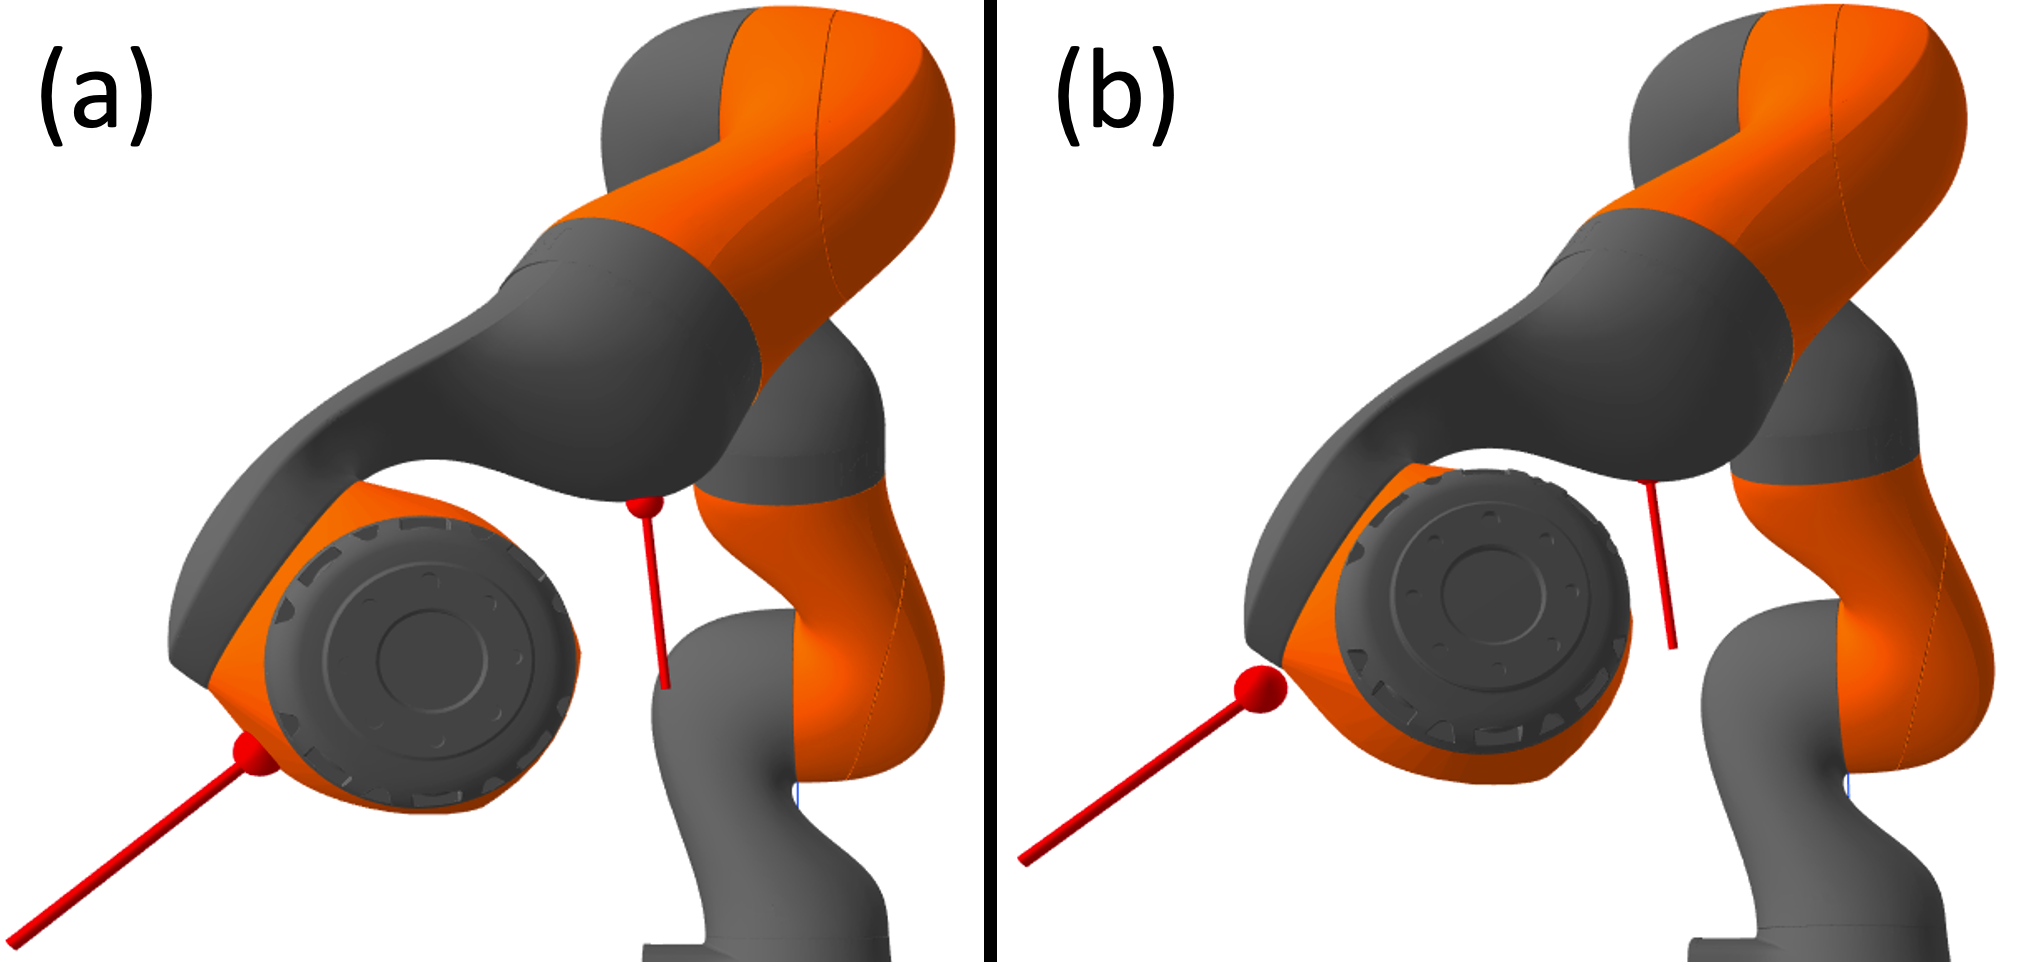
\includegraphics[width=0.75\linewidth]{figures/05_force_from_torque/active_contact_discrimination.png}
\caption{(\textbf{a}) Two possible contact positions to disambiguate. The centers of the small red spheres are coincident with the candidate contact positions. (\textbf{b}) Solving (\ref{eq:miqp}) finds a motion that pulls away from the contact on link 6 and pushes into the contact on link 5. }
\label{fig:active_contact_discrimination}
\end{figure}

There is no guarantee that this simple discrimination strategy will falsify all spurious contacts; success depends on problem specifics, e.g. robot pose, robot geometry, and the contact locations.
In particular, \eqref{eq:miqp} may return \texttt{infeasible}, or $\pull\equiv\ones$ ($\pull\equiv\mathbf{0}$) (i.e. pull/push on all contacts, which gathers no useful information). 
However, problem \eqref{eq:miqp} is a (convex) mixed-integer linear program (MILP) that can be efficiently solved to global optimality by commercial solvers. 
This means that, in the event of failure, we have a certificate that no such (sequence of) discriminating actions $\dq$ exist, at least not without relaxing the constraints \eqref{eq:miqp:pull}-\eqref{eq:miqp:lim}, or abandoning the linearized model and resorting to 
% (computationally more expensive) 
nonlinear motion planning.  

%%%%%%%%%%%%%%%%%%%%%%%%%%%%%%%%%%%%%%%%%%%%%%%%%%%%%%%%%%%%%%%%%%%%%%%%%%%%%%%%
\section{Implementation}
RSGD requires a lot more computation than existing methods. Nevertheless, by leveraging efficient open-source libraries, our implementation can run at real-time rates on a single CPU thread.

Fig. \ref{fig:run_time} shows the run-time breakdown of a typical iteration of RSGD, collected on a Mac mini with Intel i7-8700B CPU and 64GB of RAM. In Step 1, the residual $l(\cdot)$ is computed for 1000 points drawn uniformly from $S$, of which 184 points satisfy $l < \delta$. In Step 2, Algorithm \ref{algo:gradient_descent} is run on each of the 184 points until convergence, or until the limit on gradient steps is reached.
\begin{figure}[h]
\centering
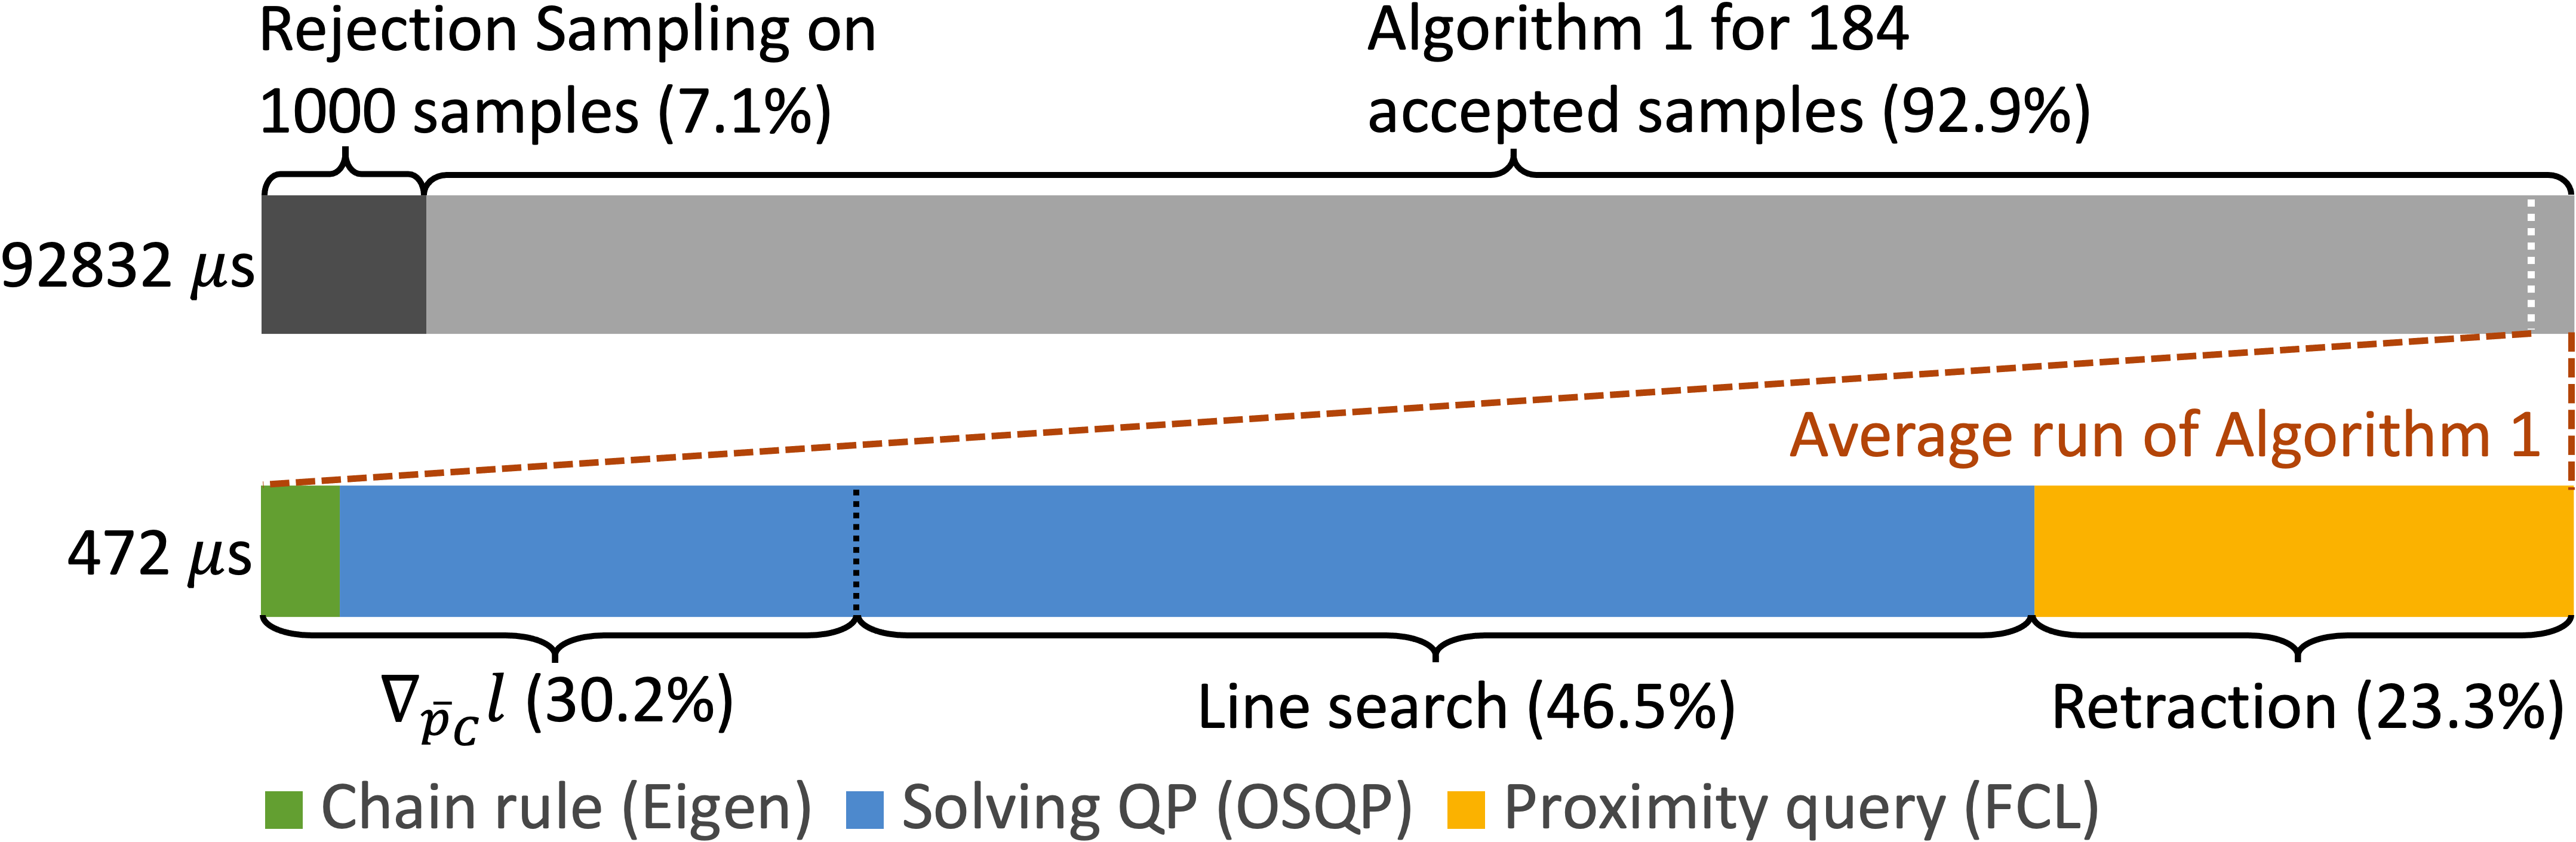
\includegraphics[width=\linewidth]{figures/05_force_from_torque/run_time.png}
\caption{Run-time breakdown of a typical iteration of RSGD.}
\label{fig:run_time}
\end{figure}

As most of the time is spent on running Algorithm \ref{algo:gradient_descent} for accepted samples in $P_\delta$, how long one iteration of RSGD takes is almost linearly proportional to $|P_\delta|$. In this case, $|P_\delta|=184$ leaves RSGD running at roughly 10Hz. This can be improved, for instance, by using a sparser $P$, putting an upper bound on $|P_\delta|$, using more CPU threads, or a combination of these strategies. 

An average run of Algorithm \ref{algo:gradient_descent} takes $472 \mu s$. The most frequently-used atomic operation is computing the residual $l(\cdot)$, which involves solving QP (\ref{eq:residual_qp:qp}). In every gradient step, $l(\cdot)$ needs to be computed once to evaluate the gradient $\nabla_{\pCbar} l(\cdot)$, and a couple more times by line search. Moreover, $l(\cdot)$ is also computed for every sample in $P$ in the earlier rejection sampling step. The lightweight QP solver OSQP\cite{stellato2020osqp} allows us to compute $l(\cdot)$ quickly: it takes $6\mu s$ on average to solve QP (\ref{eq:residual_qp:qp}). 

Retracting points back onto the robot surface $\mathcal{S}$ is the second most time-consuming operation in Algorithm \ref{algo:gradient_descent}. With the robot surface $\mathcal{S}$ represented by triangle meshes, retraction can be done efficiently by a mature proximity query routine implemented in the Flexible Collision Library (FCL) \cite{pan2012fcl}. 

The chain rule for computing $\nabla_{\pCbar} l(\cdot)$ in (\ref{eq:l_gradient_chain_rule}) is implemented with Eigen \cite{eigenweb}, which takes only 2\% of the total time needed for Algorithm \ref{algo:gradient_descent} to converge.

Algorithm \ref{algo:gradient_descent} may fail to converge if gradient descent passes through a region of $\mathcal{S}$ with almost discontinuous surface normal, e.g. a groove or an engraved letter. Proximity queries also occasionally return a point off the mesh, throwing gradient descent off its track. Nonetheless, such failures are relatively rare and easy to detect and reject when they do occur.

Concerning the active contact discrimination, although complexity of the MILP is exponential in the number of contact locations to be falsified, moderate-size problems can be solved efficiently with SOTA solvers, such as GUROBI \cite{gurobi}; e.g., a problem with $\numcontact=10$ contacts can be solved in approximately 5ms.


\section{Conclusions}
With a detailed analysis on two notions of contact detectability, we have demonstrated that a contact estimate from joint torque measurements typically consists of more than one possible contact positions, which are the global minima of the residual function $l(\cdot)$. 
Finding all global minima of $l(\cdot)$ is generally hard, but the proposed RSGD estimator empirically locates all local minima of $l(\cdot)$. 
Considering that joint torque measurements are inherently noisy, being able to find contact points with a small but positive residual could actually be beneficial. 
We have also provided a strategy to search for small robot motions which falsify as many spurious contact positions found by RSGD as possible. Moreover, when this strategy fails, it provides a certificate that no other small motion can do better.

On a robot that streams joint angle and residual torque ($\tauE$) signals, such as the KUKA IIWA, deploying RSGD is expected to be straightforward. Nevertheless, pre-processing of the raw $\tauE$ signal provided by the robot's driver, which filters out noise and ensures that the signal is unbiased, will probably be necessary.

\chapter{Contact-aware Control with Quasi-static Models} \label{chapter:quasi_static_control}
\section{Introduction}
Most robots today are programmed to move through the world as if they are afraid of making contact. Perhaps they should be: unexpected collisions while a robot is tracking a trajectory can create a large force at the point of contact, putting at risk both the robot and the environment with which it interacts (Fig. \ref{fig:contact_crushes_egg}). Consequently, a significant amount of effort and care in robot motion planning is spent on avoiding collisions. For example, sampling-based planners need to perform numerous collision checks \cite{lavalle2006planning}; optimization-based planners need to constantly evaluate the signed distance functions and their gradients \cite{ratliff2009chomp}. Moreover, high resolution collision geometries are usually needed to increase the chances of finding a collision-free path, which further increases the computational cost \cite{pan2012fcl}.

However, the complete and total avoidance of contacts is a severe limitation, even if we are willing to tolerate the computational cost. First, the effectiveness of collision-free planning is limited by the quality of the geometric models used for collision checks. Unless in structured environments where everything has been perfectly measured, models of the environment need to be reconstructed from range sensor (e.g. depth camera) measurements, which usually have a fair amount of uncertainty and can suffer from occlusion. Moreover, collision-free trajectories can be unnecessarily conservative \cite{mason2018toward}: a task achievable by making some contacts can be deemed infeasible by a collision-free planner. 
\begin{figure}
    \centering
    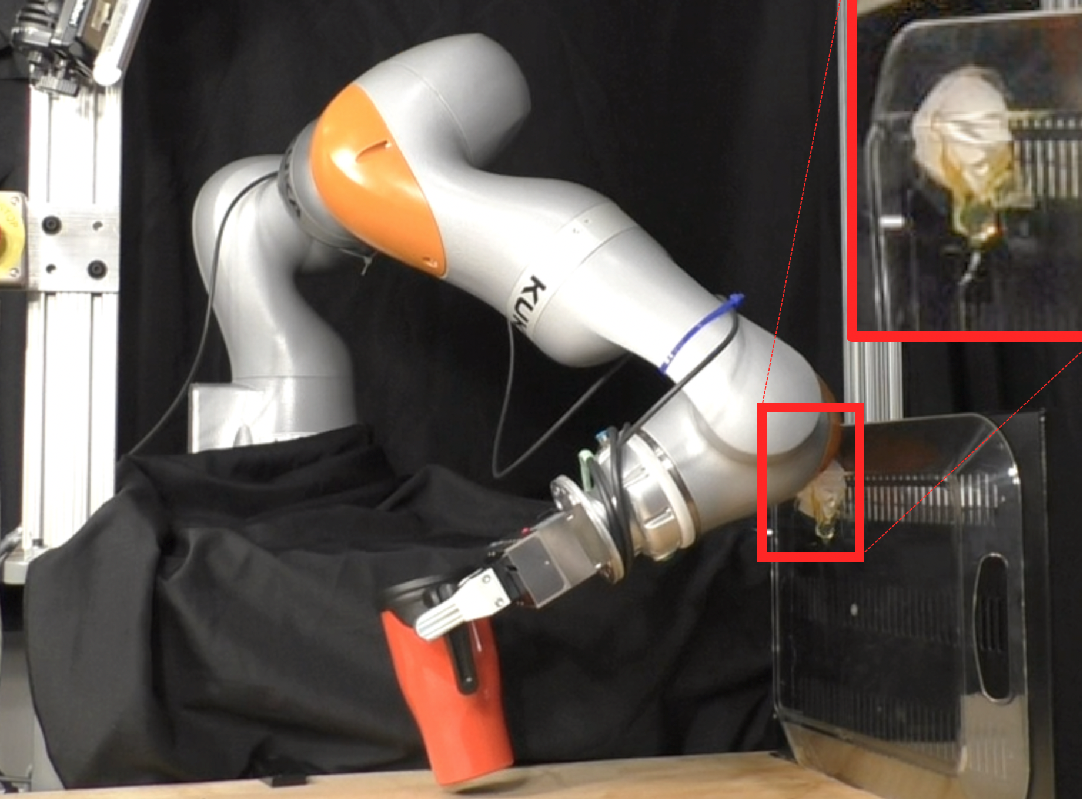
\includegraphics[width=0.65\linewidth]{figures/04_control/figure1.png}
    \caption{As transparent obstacles are almost invisible to depth sensors, a collision-free motion planner, with the goal to pick up the mug and unaware of the transparent tray, plans a trajectory that crushes the egg along the way. The crushed egg is highlighted in the red box. Our controller is able to keep the egg intact even when the reference trajectory would crush it.}
    \label{fig:contact_crushes_egg}
    % \vspace{-0.7cm}
\end{figure}

In this chapter, we propose a QP controller which, given estimated contact positions and forces in unexpected contacts, tracks the reference trajectory as closely as possible while keeping contact forces below a user-defined upper bound.
Compared with similar controllers based on null-space projection \cite{nakamura1987task, siciliano1991general, aghili2005unified, dehio2018modeling, jorda2019contact}, the QP formulation shares the same underlying dynamics, but allows for more gentle separation when the robot breaks contact with the environment. The gentle separation happens naturally as a result of bounding the contact forces with inequality constraints, which are not supported by null-space projection.

Instead of the usual second-order dynamics constraints used in robot locomotion \cite{kuindersma2014efficiently, koolen2016design}, the proposed QP controller utilizes a quasistatic dynamics model which predicts future equilibrium configurations and contact forces for a stiffness-controlled robot in response to position commands. By assuming bi-lateral, frictionless contacts, the quasistatic dynamics model can be expressed as equality constraints and does not require the estimation of friction coefficients. Moreover, as real-world contacts are uni-lateral and frictional, we also propose measures which both capitalize the simplicity of bi-lateral, frictionless contact models and mitigate the side effects of modeling real-world contacts as such.


\section{Related Work  \label{sec:related_work}}
\subsection{Interaction Control}
As the primary objective of the proposed QP controller is to bound unexpected contact forces while tracking a joint-space or end-effector trajectory, we review existing methods for combined motion and force control, which are also referred to as interaction control in the literature \cite[Chapter~9]{siciliano2008springer}. Interaction control techniques can be broadly classified by whether the interaction force is controlled \textit{directly} or \textit{indirectly}. 

Direct force control typically splits the task space into two orthogonal subspaces based on the robot's kinematic constraints: one motion-controlled subspace along the tangents of the kinematic constraints, and one force-controlled subspace along the normals. Desired motion and force trajectories are specified in the motion and force controlled subspaces, and tracked independently using motor torque commands computed from the robot's second-order model \cite{mason1981compliance, khatib1987unified, raibert1981hybrid}. 

However, the success of direct force control relies on accurate robot and environment models, which are not easily available in unstructured environments. Moreover, with few exceptions \cite{franka}, most industrial robot arms, including the KUKA iiwa, do not have an interface for end-users to directly control motor torques \cite{kuka2019fri}. Last but not least, by directly controlling motor torque, the interaction controller bypasses the robot's factory motion controller, and thus needs to run at high frequency in order to maintain stability.

On the other hand, a classical example of indirect force control is impedance control \cite{hogan1984impedance}, which regulates the robot's response to external forces to that of a mass-spring-damper system (a mechanical impedance), thereby guaranteeing interaction stability by passivity. When the robot moves slowly, which is often the case in manipulation tasks, impedance control can be simplified to stiffness control \cite{salisbury1980active}, which can be interpreted as connecting the robot's end effector to a user-specified set-point by virtual springs. In the presence of contact, contact force can be controlled by commanding how much the set point penetrates the obstacle.

Compared with direct force control, indirect force control schemes are usually implemented as an outer-loop around the robot's factory motion controller, and therefore does not bear the responsibility of maintaining stability and can run at a much lower rate.

\subsection{Quasi-static Dynamics Models in Manipulation}
Quasistatic dynamics has been used with great success to simplify the planning and control of simple tasks such as planar pushing \cite{hogan2020feedback}, where modeling robots as prescribed motion trajectories is sufficient. However, for multi-contact tasks such as grasping \cite{pang1996complementarity}, such simplifications can lead to non-unique contact forces  or violation of non-penetration constraints \cite{halm2018quasi, pang2018robust}. By modeling robots as impedances, our recent multibody quasistatic model \cite{pang2021convex} can faithfully reproduce the steady-state behavior of stiffness-controlled robot arms in multi-contact scenarios.

The quasistatic robot dynamics model proposed in this work, which predicts future joint angles in whole-arm contact scenarios, is an extension to classical indirect force control schemes that typically focus solely on the relationship between end effector pose and wrench \cite{salisbury1980active, hogan1984impedance}. The proposed quasistatic dynamics is also a frictionless simplification of the Coulomb-friction-based quasistatic dynamics \cite{pang2021convex}, which can be implemented on hardware with minimal contact sensing.


\subsection{Null-space Projection}
Null-space projection is a classical and popular technique for executing a hierarchy of tasks defined by equality constraints \cite{nakamura1987task, siciliano1991general, aghili2005unified, dehio2018modeling, jorda2019contact}. The constraints imposed by higher-priority tasks are enforced by projecting the torque needed by low-priority tasks into the null space of the higher-priority tasks. The projections are defined over the ranges and null spaces of the task Jacobians and their \textit{weighted} pseudo-inverses. It is noteworthy that the projections are generally not orthogonal, unless the weight matrix is identity \cite{dietrich2015overview}.

More recently, controllers based on constrained optimizations such as quadratic programs (QP) have gained popularity in both locomotion \cite{koolen2016design, kuindersma2014efficiently} and manipulation \cite{jain2013manipulation}. Compared with null-space projections, QP-based controllers can handle both equality and inequality constraints. In this work, we formulate the problem of trajectory tracking with bounded contact forces as a QP with a novel quasistatic dynamics constraint. We also show that a controller based on null-space projection implicitly enforces the same quasistatic dynamics constraint when the projection is \textit{stiffness-consistent} \cite{dietrich2015overview}.


\section{Background and Notations}
\subsection{Constrained Inverse Dynamics Control}
A popular controller in locomotion and manipulation is based on the following optimization-based formulation \cite{kuindersma2014efficiently, koolen2016design, wang2019impact}:
\begin{subequations}
\label{eq:generic_mpc}
\begin{align}
\underset{x^{l+1}, u^l}{\text{min.}} \; &c_x(x^{l+1}) + c_u(u^l), \; \text{s.t.}\\
&x^{l+1} = f(x^{l}, u^l), \label{eq:generic_mpc:dynamics_constraint}
\end{align}
\end{subequations}
where $x^{l}$ and $u^{l}$ are the state and input at the current time step $l$, and $x^{l+1}$ is the state at the next time step, $l+1$. The controller (\ref{eq:generic_mpc}) picks an action $u^l$ that minimizes the (usually LQR-style) state and action cost, $c_x(\cdot)$ and $c_u(\cdot)$, subject to the dynamics constraint (\ref{eq:generic_mpc:dynamics_constraint}).

The most common choice for the dynamics constraint (\ref{eq:generic_mpc:dynamics_constraint}) is the Newton's Second Law (N2L). For example, the DLR (German Aerospace Center) family of robots, including the KUKA iiwa and FRANKA panda, has the following closed-loop second-order dynamics after gravity compensation\cite{ott2008passivity}: 
\begin{equation}
\label{eq:iiwa_second_order_closed_loop_dynamics}
M(q) \ddot{q} + \left(C(q, \dot{q}) + D_q\right) \dot{q} + K_q(q - \qcmd) = \tauE,
\end{equation}
where $q \in \mathbb{R}^{n_q}$ is the joint angles of the robot, $C(q, \dot{q}) \dot{q}$ is the Coriolis force, $D_q$ is a diagonal damping matrix, $K_q$ is a diagonal stiffness matrix, $\qcmd$ is the commanded joint angles, and $\tauE$ is the torque by external contacts.

\subsection{Contact and Multibody Notations}
We consider rigid, point contacts in this work. The number of contacts the robot makes with the environment is denoted by $n_c$. Each contact point is denoted by $C_i$. The coordinates of the contact point relative to world frame, expressed in world frame is written as $\quantity{p}{W}{C_i}{} \in \mathbb{R}^3$; contact force at $C_i$ expressed in world frame is represented by $\quantity{f}{}{C_i}{W} \in \mathbb{R}^3$. 

Position Jacobian of the contact point $C_i$ relative to frame $W$, expressed in frame $W$, is denoted by $J_{q}^{\quantity{p}{W}{C_i}{}}(q) : \mathbb{R}^{n_q} \rightarrow \mathbb{R}^{3 \times n_q}$. It maps the robot's joint velocity $\Dot{q}$ to the velocity of point $C_i$ in world frame $W$:
\begin{equation}
\quantity{v}{W}{C_i}{} = J_{q}^{\quantity{p}{W}{C_i}{}}(q) \Dot{q}.
\end{equation}

We further define
\begin{subequations}
\label{eq:contact_definitions}
\begin{align}
f_i  &\coloneqq \norm{\quantity{f}{}{C_i}{W}} \in \mathbb{R};  \;  u_i \coloneqq \quantity{f}{}{C_i}{W} / f_i \in \mathbb{R}^3\\
J_{u_i} &\coloneqq u_i^{\intercal} J_{q}^{\quantity{p}{W}{C_i}{}} \in \mathbb{R}^{1 \times n_q}\\
J_u &\coloneqq \left[J_{u_1}^\intercal, J_{u_2}^\intercal, \cdots J_{u_{n_c}}^\intercal \right]^\intercal \in \mathbb{R}^{n_c \times n_q}. \label{eq:contact_jacobian}
\end{align}
\end{subequations}
The $i$-th row of $J_u$ maps $\Dot{q}$ to the Cartesian velocity of $C_i$ along $u_i$ in world frame. We assume that $J_u$ is full-rank.


\section{Quasi-static Dynamics}
\subsection{Dynamics as Transitions between Equilibria \label{sec:quasistatic_dynamics_1}}
For robot arms with a joint-level stiffness controller, their steady-state equilibrium condition can be obtained by setting the derivative terms in the second-order dynamics (\ref{eq:iiwa_second_order_closed_loop_dynamics}) to 0:
\begin{equation}
\label{eq:quaistatic_force_balance}
K_q (\qcmd - q) + \tauE = 0. 
\end{equation}

For a stiffness-controlled robot, we can define its \textit{quasi-static} dynamics, whose state consists only of the joint angles $q$, and input the commanded joint angles $\qcmd$. As shown in Fig. \ref{fig:quasistatic_dynamics}, the quasistatic dynamics predicts $x^{l+1} \coloneqq q^{l+1}$, the equilibrium configuration at the next time step, from the current equilibrium configuration $q^{l}$ and the next commanded configuration $u^l \coloneqq \qcmd[l+1]$.
\begin{figure}[h]
\vspace{-0.3cm}
\centering
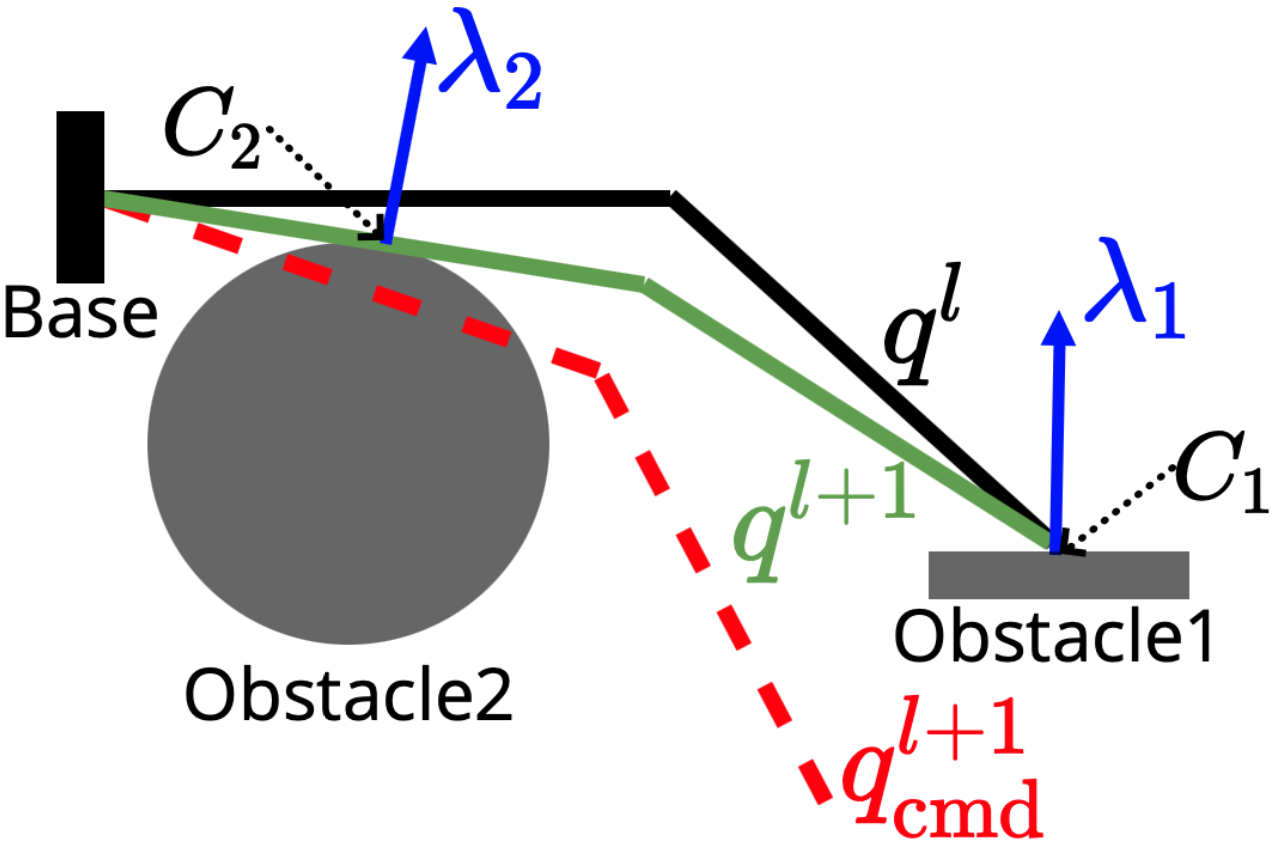
\includegraphics[width=0.45\linewidth]{figures/04_control/quasistatic_dynamics.png}
\caption{Quasistatic dynamics of a 2D, 2-link robot arm. The arm starts at $q^l$ (black) and is commanded to go to $\qcmd[l+1]$ (red). The virtual spring connecting $\qcmd[l+1]$ to $q^l$ pulls the robot towards $\qcmd[l+1]$, but the robot eventually stabilizes to $q^{l+1}$ (green) due to contact constraints. At $l+1$, the arm makes two contact with two obstacles at $C_1$ and $C_2$ with contact forces $\lambda_1$ and $\lambda_2$.}
\label{fig:quasistatic_dynamics}
\vspace{-0.3cm}
\end{figure}

The new equilibrium $q^{l+1}$ can be solved for by minimizing the potential energy of the robot, subject to the contact constraints:
\begin{subequations}

\label{eq:quasistatic_dynamics_qp}
\begin{align}
\underset{q^{l+1}}{\text{min.}} \; &\frac{1}{2}(\qcmd[l+1] - q^{l+1})^\intercal K_q (\qcmd[l+1] - q^{l+1}) \; \text{s.t.} \\
& J_u(q^l) (q^{l+1} - q^{l}) = 0. \label{eq:quasistatic_dynamics_qp:equality_constraint}
\end{align}
\end{subequations}

To derive the contact forces, we start with the Lagrangian of QP (\ref{eq:quasistatic_dynamics_qp}):
\begin{equation}
\begin{aligned}
L(q^{l+1}, \lambda) = &\frac{1}{2} (\qcmd[l+1] - q^{l+1})^\intercal K_q (\qcmd[l+1] - q^{l+1}) \\
&- (\lambda^{l+1})^\intercal J_u(q^{l+1} - q^l)
\end{aligned}
\end{equation}
where $\lambda^{l+1} \in \mathbb{R}^{n_c}$ is the Lagrange multipliers of the contact constraint (\ref{eq:quasistatic_dynamics_qp:equality_constraint}), which can also be interpreted as the contact forces generated by (\ref{eq:quasistatic_dynamics_qp:equality_constraint}); the dependency of $J_u$ on $q^l$ is dropped for simplicity.

The KKT optimality condition of QP (\ref{eq:quasistatic_dynamics_qp}) is given by
\begin{subequations}

\label{eq:dynamics_qp_kkt}
\begin{align}
\nabla_{q^{l+1}}L = K_q (q^{l+1} - \qcmd[l+1]) - J_u^\intercal \lambda^{l+1} &= 0, \label{eq:dynamics_qp_kkt:gradient} \\
  J_u \left(q^{l+1} - q^l\right) &= 0. \label{eq:dynamics_qp_kkt:equality_constraint}
\end{align}
\end{subequations}
where (\ref{eq:dynamics_qp_kkt:gradient}) is equivalent to the steady-state force balance condition (\ref{eq:quaistatic_force_balance}), assuming that $\tauE$ is generated by the $n_c$ point contacts, i.e. $\tauE = J_u^\intercal \lambda^{l+1}$.

Explicit expressions for $\lambda^{l+1}$ and $q^{l+1}$ can also be derived from the KKT conditions (\ref{eq:dynamics_qp_kkt}):
\begin{subequations}

\label{eq:explicit_force_and_state}
\begin{align}
\lambda^{l+1} &= -(J_u K_q^{-1} J_u^\intercal)^{-1} J_u (\qcmd[l+1] - q^l), \label{eq:explicit_force_and_state:force}\\
q^{l+1} &= q^l + \left(I -  K_q^{-1}J_u^\intercal (J_u K_q^{-1} J_u^\intercal)^{-1}J_u \right) (\qcmd[l+1] - q^l). \label{eq:explicit_force_and_state:state}
\end{align}
\end{subequations}


\subsection{Relationship to Null-space Projection}
In this sub-section, we show that when controlling stiffness-controlled robots using null-space projection, lower-priority tasks can be guaranteed to not interfere with higher-priority tasks during transients if the stiffness-consistent projection \cite{dietrich2015overview} is used. We also show that the underlying dynamics model of a controller based on stiffness-consistent projection is the same as the model proposed in Sec. \ref{sec:quasistatic_dynamics_1}. 

Null-space projection technique revolves around two projections: 
\begin{subequations}

\begin{align}
P_R(W) &\coloneqq J_u^\intercal \left(J_u^{W +}\right)^\intercal, \\
P_N(W) &\coloneqq I - J_u^\intercal \left(J_u^{W +}\right)^\intercal,
\end{align}
\end{subequations}
where $J_u^{W+} \coloneqq W^{-1} J_u^\intercal (J_u W^{-1} J_u^\intercal)^{-1}$ is the pseudo-inverse weighted by a positive-definite $W$. The range and null space of $P_R(W)$ are respectively $R(J_u^\intercal)$ and $N\left(\left(J_u^{W+}\right)^\intercal\right)$, whereas the range and null space of $P_N(W)$ are reversed. Note that such projections can be defined for arbitrary task Jacobians, but we specialize to the contact Jacobian defined in (\ref{eq:contact_jacobian}) without loss of generality.

For any choice of $W$ and any joint torque $\tauM$, $P_R(W) \tauM \in R(J_u^\intercal)$ generates contact forces, whereas $P_N(W) \tauM$ generates no joint torque in $R(J_u^\intercal)$ after static equilibrium is reached. Choosing an appropriate $W$, however, can provide additional guarantees during the transient into this steady state \cite{dietrich2015overview}. For instance, the \textit{dynamically-consistent} pseudo-inverse $J_u^{M+}$\cite{featherstone1997load}, which uses the robot's mass matrix $M$ for $W$, ensures that 
\begin{equation}
\label{eq:dynamic_consistency}
0 \equiv J_u M^{-1} P_N(M) \tauM, \; \forall \tauM.
\end{equation}
Assuming that the dominant effect of $P_N(M) \tauM$ during the transient is to generate acceleration, property (\ref{eq:dynamic_consistency}) guarantees that and the generated acceleration lies inside $N(J_u)$.

% Analysis for quasi-static systems.
To determine the appropriate choice of $W$ when the dominant effect of the $P_N(W) \tauM$ during transient is to stretch/contract the virtual spring of a stiffness-controlled robot, we start at the instant $l^+$, immediately after sending the joint angle command $u^l = \qcmd[l+1]$ at time step $l$. At $l^+$, the joint torque can be expressed as 
\begin{equation}
\label{eq:tau_l_stiffness}
\tauM^{l^+} = K_q(\qcmd[l+1] - q^l),
\end{equation}
which can be decomposed as 
\begin{equation}
\label{eq:tau_l_decomposition}
\tauM^{l^+} = \underbrace{P_R(W) \tauM^{l^+}}_{\tau_R} + \underbrace{P_N(W) \tauM^{l^+}}_{\tau_N},
\end{equation}
where $\tau_R \in R(J_u^\intercal)$ generates contact forces, and $\tau_N \in N\left(\left(J_u^{W+}\right)^\intercal\right)$ generates a motion that needs to be in $N(J_u)$.

Combining (\ref{eq:tau_l_stiffness}) and (\ref{eq:tau_l_decomposition}) yields
\begin{equation}
\label{eq:tau_l_combined}
K_q(\qcmd[l+1] - q^l) = \tau_R +\tau_N.
\end{equation}

At time instant $(l+1)^-$, when the equilibrium at time step $l+1$ is reached but $u^{l+1}$ has not been commanded, $\tau_N$ has generated a displacement and been dissipated by damping, but $\tau_R$, the generalized force due to contact, remains:
\begin{equation}
\label{eq:tau_l+1_decomposition}
\tauM^{(l+1)^-} = \tau_R.
\end{equation}
Moreover, static equilibrium (\ref{eq:quaistatic_force_balance}) at $(l+1)^-$ dictates that 
\begin{equation}
\label{eq:tau_l+1_stiffness}
\tauM^{(l+1)^-} = K_q(\qcmd[l+1] - q^{l+1}).
\end{equation}

Combining (\ref{eq:tau_l+1_decomposition}) and (\ref{eq:tau_l+1_stiffness}) yields 
\begin{equation}
\label{eq:tau_l+1_combined}
K_q(\qcmd[l+1] - q^{l+1}) = \tau_R.
\end{equation}

Finally, subtracting (\ref{eq:tau_l+1_combined}) from (\ref{eq:tau_l_combined}) gives
\begin{equation}
\label{eq:stiffness_consistency_1}
K_q(q^{l+1} - q^l) = \tau_N = P_N(W) \tauM^{l^+}.
\end{equation}

As the motion from $l$ to $l+1$ needs to stay in $N(J_u)$, we need $J_u(q^{l+1} - q^l) \equiv 0$, which implies through (\ref{eq:stiffness_consistency_1}) that
\begin{equation}
0 \equiv J_u K_q^{-1}P_N(W) \tauM^{l^+}, \; \forall \tauM^{l^+},
\end{equation}
which has the same form as dynamic-consistency defined in (\ref{eq:dynamic_consistency}). Not surprisingly, choosing $W = K_q$ ensures the motion generated by $\tau_N$ stays in $N(J_u)$, and the resulting pseudo-inverse $J^{K_q+}$ is called \textit{stiffness-consistent} \cite{dietrich2015overview}.

We can solve for $q^{l+1}$ by plugging (\ref{eq:tau_l_stiffness}) into (\ref{eq:stiffness_consistency_1}) and setting $W$ to $K_q$, yielding
\begin{equation}
\label{eq:state_null_space_projection}
q^{l+1} = q^l + (I - J_u^{K_q+}J_u) (\qcmd[l+1] - q^l).
\end{equation}

Furthermore, as the contact force is the reaction to $\tau_R$, we have $\tau_R = -J_u^\intercal \lambda^{l+1}$, combining this with the definition of $\tau_R$ in (\ref{eq:tau_l_decomposition}) gives
\begin{equation}
\label{eq:force_null_space_projection}
\lambda^{l+1} = -\left(J^{K_q+} \right)^\intercal K_q(\qcmd[l+1] - q^l).
\end{equation}

It can be shown that (\ref{eq:state_null_space_projection}) and (\ref{eq:force_null_space_projection}) are equivalent to (\ref{eq:explicit_force_and_state:state}) and (\ref{eq:explicit_force_and_state:force}), respectively. This equivalence implies that a controller based on stiffness-consistent projections and a controller (\ref{eq:generic_mpc}) using QP (\ref{eq:quasistatic_dynamics_qp}) as its dynamics constraint share the same underlying dynamics model. Therefore, the QP formulation in Sec. \ref{sec:MPC} is preferred as it can handle inequality constraints.


\section{QP Controller with Quasistatic Dynamics \label{sec:MPC}}
\subsection{Frictionless Contacts}
To track a reference trajectory $q_\text{ref}(t)$ as closely as possible while respecting dynamics constraints and upper bounds on contact forces, we can specialize the generic optimization-based controller (\ref{eq:generic_mpc}) to the following QP:
\begin{subequations}
\label{eq:mpc_qp1}
\begin{align}
\underset{q^{l+1}, q_{\text{cmd}}^{l+1}, \lambda^{l+1}} {\rm min} \; &\left\|q^{l+1} - q_\text{ref}^{l+1}\right\|^2 + 
\epsilon \left\|q_{\rm cmd}^{l+1} - q_\text{ref}^{l+1}\right\|^2 , \text{s.t.} \label{eq:mpc_qp1:objective} \\
&K_q(q^{l+1} - q_\text{cmd}^{l+1}) - J_u^\intercal \lambda^{l+1} = 0 \label{eq:mpc_qp:dynamics1}\\
&J_u(q^{l+1} - q^l) = 0 \label{eq:mpc_qp:dynamics2}\\
&\lambda^{l+1} \leq \lambda_\text{max} \label{eq:mpc_qp:force_upper_bound}\\
&\left|q_\text{cmd}^{l+1} - \qcmd[l]\right| \leq \Delta q_\text{max}. \label{eq:mpc_qp:velocity_upper_bound}
\end{align}
\end{subequations}
Here, the dynamics constraint (\ref{eq:generic_mpc:dynamics_constraint}) consists of (\ref{eq:mpc_qp:dynamics1}) and (\ref{eq:mpc_qp:dynamics2}), which are the KKT conditions (\ref{eq:dynamics_qp_kkt}) of the quasistatic dynamics (\ref{eq:quasistatic_dynamics_qp}). Constraint (\ref{eq:mpc_qp:force_upper_bound}) places an upper bound on contact forces. The last constraint (\ref{eq:mpc_qp:velocity_upper_bound}) bounds how quickly $\qcmd$ changes.

In the objective (\ref{eq:mpc_qp1:objective}), the first term penalizes deviation at $l+1$ from the reference trajectory. The second term, weighted by a small positive scalar $\epsilon$, adds regularization without which the objective would become semi-definite. To see why, we re-write $\left(q^{l+1} - q_\text{ref}^{l+1}\right)$ by expressing $q^{l+1}$ explicitly as a function of $q_\text{cmd}^{l+1}$ using (\ref{eq:state_null_space_projection}):
\begin{equation}
\label{eq:q_minus_q_ref}
q^{l+1} - q_\text{ref}^{l+1} = (I - J_u^{K_q+}J_u) (q^{l+1}_\text{cmd} - q^l) + (q^{l} - \qref[l+1]),
\end{equation}
where the second term is a constant, and the first term multiplies $(q_\text{cmd}^{l+1} - q^l)$ by a projection which has a non-zero null space.

In the quasistatic dynamics (\ref{eq:quasistatic_dynamics_qp}), expressing contact constraints as equality constraints (\ref{eq:quasistatic_dynamics_qp:equality_constraint}) and contact forces as the constraints' Lagrange multipliers implies that the contacts are bi-lateral and frictionless. In reality, however, contacts are uni-lateral and frictional.


The bi-lateralness of (\ref{eq:quasistatic_dynamics_qp:equality_constraint}) is less concerning. As contact sensors are inevitably noisy, only contact forces above a threshold are added to QP (\ref{eq:mpc_qp1}). In addition, by (\ref{eq:explicit_force_and_state:force}), the change in contact force is bounded as long as $\left|\qcmd[l+1] - q^l\right|$ is bounded, and the boundedness of $\left|\qcmd[l+1] - q^l\right|$ is enforced by (\ref{eq:mpc_qp:velocity_upper_bound}). Therefore, as long as the bound $\Delta q_\text{max}$ is sufficiently small, we do not need to worry about contact forces flipping sign in the middle of a control step. 

On the other hand, naively ignoring friction will severely impact the performance of the controller, which motivates the mitigating measures detailed in the next subsection.

\subsection{Frictional Contacts}
It is possible to model friction contact in quasistatic dynamics \cite{pang2021convex}, but control through a frictional contact requires estimating the contact normal and the friction coefficient, in addition to estimating contact forces. This requires either more sophisticated whole-arm contact sensors, or making additional assumptions about the environments that make the control-estimation pipeline more brittle. 

Therefore, we will retain the simpler frictionless contact model for controlling through a frictional contact, and mitigate the side effects of the wrong contact model by modifying the frictionless QP (\ref{eq:mpc_qp1}) to
\begin{subequations}
\label{eq:mpc_qp2}
\begin{align}
\underset{q^{l+1}, q_{\text{cmd}}^{l+1}, \lambda^{l+1}} {\rm min} \; &\underbrace{\left\|q_\text{cmd}^{l+1} - q_\text{ref}^{l+1}\right\|^2}_{\text{tracking}} + \underbrace{
w^l \left\|q_\text{cmd}^{l+1} - q_\text{cmd}^{l}\right\|^2}_{\text{damping}} \label{eq:mpc_qp2:objective}, \; \text{s.t. } \\
&\text{(\ref{eq:mpc_qp:dynamics1}), (\ref{eq:mpc_qp:dynamics2}), (\ref{eq:mpc_qp:force_upper_bound}) and (\ref{eq:mpc_qp:velocity_upper_bound}),} \nonumber
\end{align}
\end{subequations}
which has the same constraints as (\ref{eq:mpc_qp1}) but a different objective. In the rest of this section, we will elaborate on the reason for both terms in the objective (\ref{eq:mpc_qp2:objective}).

\subsubsection{Tracking}
When the reference trajectory $q_\text{ref}^{l+1}$ leads the robot to make contact with a frictional surface at point $C$ (Fig. \ref{fig:frictional_contact_objective}a), the surface normal $n \in \mathbb{R}^3$ and the contact force direction $u \in \mathbb{R}^3$ can be different. However, the frictionless contact model (\ref{eq:mpc_qp:dynamics1})-(\ref{eq:mpc_qp:dynamics2}) assumes that $u$ is always the same as $n$. Therefore, it is possible for ${}^W v^C_\text{cmd}$, the commanded velocity of $C$, to have a negative component along $u$ but a positive component along $n$, as shown in Fig. \ref{fig:frictional_contact_objective}a. Such a ${}^W v^C_\text{cmd}$ would lead to the robot separating from the obstacle at $l+1$. When the frictionless QP (\ref{eq:mpc_qp1}) is constructed again at $l+1$, no contact force constraints are added but $q_\text{ref}^{l+2}$ can still lead the robot to contact with a large amount of penetration. Therefore, the robot could re-establish contact with a large contact force at $l+2$.

Although it is difficult to guarantee that ${}^W v^C_\text{cmd}$ has a negative component along $n$ without knowing $n$, undesired contact jitters can be effectively reduced by making ${}^W v^C_\text{cmd}$ as close as possible to ${}^W v^C_\text{ref}$. In joint space, this translates to minimizing the distance between $\qcmd[l+1]$ and $\qref[l+1]$, which can be achieved by replacing the term $\left\|q^{l+1} - q_\text{ref}^{l+1}\right\|^2$ in (\ref{eq:mpc_qp1:objective}) by $\left\|q_\text{cmd}^{l+1} - q_\text{ref}^{l+1}\right\|^2$ in (\ref{eq:mpc_qp2:objective}).

To further illustrate the advantage of the new objective, we first re-write $q_\text{cmd}^{l+1} - q_\text{ref}^{l+1}$ using the relative quantities defined in Fig. \ref{fig:frictional_contact_objective}b:
\begin{equation}
q_\text{cmd}^{l+1} - \qref[l+1] = \left(q_\text{cmd}^{l+1} - q^l \right) - \left(\qref[l+1] - q^l \right) = \Delta q_\text{cmd}^{l+1} - \Delta \qref[l+1].
\end{equation}

It is also easy to see from (\ref{eq:q_minus_q_ref}) that
\begin{equation}
\Delta q^{l+1} = (I - J_u^{K_q+}J_u) \Delta q_\text{cmd}^{l+1}.
\end{equation}
The first term in the original objective (\ref{eq:mpc_qp1:objective}) thus becomes
\begin{equation}
\begin{aligned}
q^{l+1} - \qref[l+1] =& \Delta q^{l+1} - \Delta \qref[l+1] \\
=& (I - J_u^{K_q+}J_u) \Delta q_\text{cmd}^{l+1} - \Delta \qref[l+1],
\end{aligned}
\end{equation}
where $(I - J_u^{K_q+}J_u)$ is the projection into $N(J_u)$ along $R\left(J_u^{K_q+}\right)$, as shown in Fig. \ref{fig:frictional_contact_objective}b. 

As a result, minimizing $\norm{\Delta q_\text{cmd}^{l+1} - \Delta \qref[l+1]}^2$ encourages $\Delta q_\text{cmd}^{l+1}$ to be close to $\Delta \qref[l+1]$ in the entire vector space. In contrast, when $\norm{\Delta q^{l+1} - \Delta \qref[l+1]}^2$ is used as the cost, only the distance between $\Delta \qref[l+1]$ and the component of $\Delta q_\text{cmd}^{l+1}$ along $N(J_u)$ is minimized.

\begin{figure}[h]
\centering
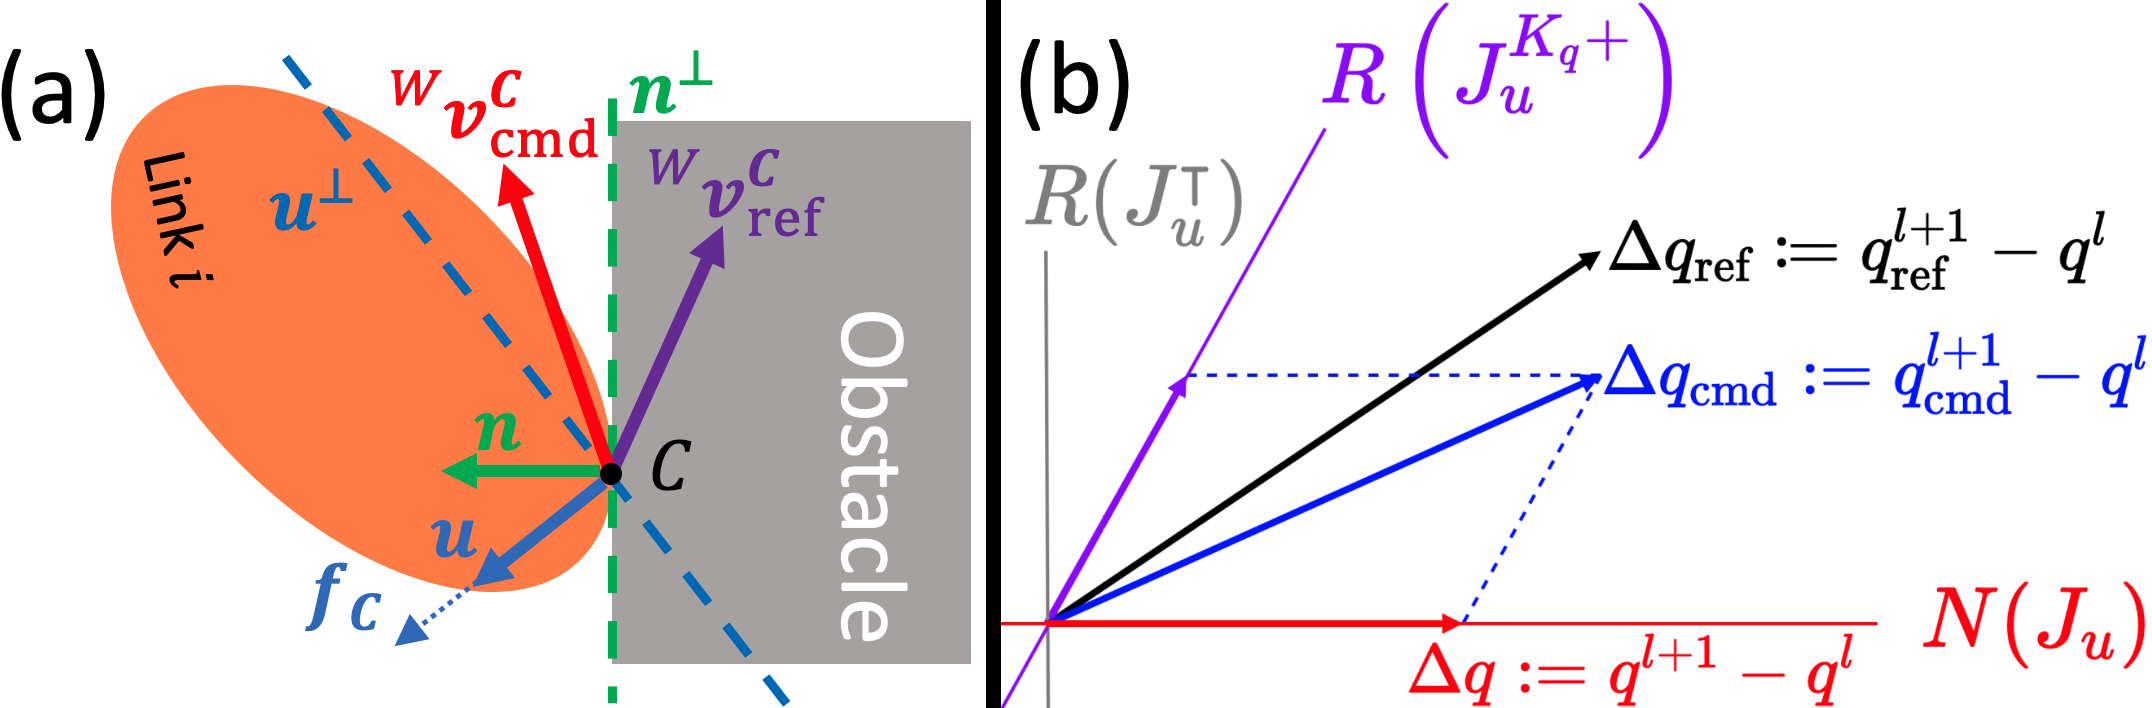
\includegraphics[width=0.80\linewidth]{figures/04_control/frictional_contact_objective.png}
\caption{\textbf{(a)}: The reference trajectory brings the robot into contact at $C$. Due to friction, the contact normal $n$ and the contact force direction $u$ are different. Therefore, the commanded velocity at $C$ can separate from the obstacle even when the angle between $u$ and ${}^W v^C_\text{cmd}$ is greater than $\pi / 2$. \textbf{(b)}: Definitions of $\Delta q_\text{ref}$, $\Delta q_\text{cmd}$ and $\Delta q$. The range and null space of the projection $I - J_u^{K_q+}J_u$ are $N(J_u)$ and $R\left(J_u^{K_q+}\right)$, respectively.}
\label{fig:frictional_contact_objective}
\end{figure}

\begin{figure*}[t!]
\vspace{0.2cm}
\centering
\includegraphics[width=1.0\textwidth]{figures/04_control/experiments_high_res.png}
\caption{(\textbf{a}): mug placement task. (\textbf{b}): mug moving task. Contacts are highlighted in red boxes. Blue arrows denote the direction of end effector velocity. For both tasks, the photographs on the left show where the real robot makes contact while executing the task. With collision geometry disabled, the simulation frames on the right show how much penetration would happen if the original trajectory were strictly followed. Videos of the real robot executing the tasks are included in the attachment.}
\label{fig:experiments}
\vspace{-0.6cm}
\end{figure*}


\subsubsection{Damping} 
The goal of this term is to command more conservative robot motions when we are less confident in the correctness of the frictionless contact model. As real-world contacts are almost always frictional, the contact force predicted by the frictionless model and the actual contact force measured by contact sensors are bound to be different. At every time step, this discrepancy can be quantified by
\begin{equation}
e_\lambda^l \coloneqq 1 - \exp{\left(\left\|\lambda_{\rm pred}^l -\lambda_{\rm est}^l \right\|_{\infty}/a\right)} \in [0, 1],
\end{equation}
where $\lambda_{\rm pred}^l$ is the contact forces predicted by the frictional QP (\ref{eq:mpc_qp2}) at time step $l - 1$; $\lambda_{\rm est}^l$ is the measured contact forces at time step $l$; $a$ is a positive constant that weights the force prediction error. The discrepancy $e_\lambda$ is close to $1$ when the force prediction error is large, and close to $0$ when the error is small.

The weight of the second term of (\ref{eq:mpc_qp2:objective}), $w^l$, is the low-pass-filtered version of the discrepancy $e_\lambda^l$:
\begin{equation}
w^l = w_\text{max} \left[ \alpha e_\lambda^l + (1 - \alpha) e_\lambda^{l-1} \right],
\end{equation}
where $w_\text{max}$ is the upper bound on $w^l$ and $\alpha$ is the forget rate of the low-pass filter. A larger $w^l$ encourages more conservative robot motions by more heavily penalizing the change in $\qcmd$ from $l$ to $l+1$.


\section{Experiments}
In this section, we demonstrate the advantages of the proposed contact-aware controller through two tasks that involve unexpected contact with the environment, which are shown in Fig. \ref{fig:experiments}. In both experiments, $\qcmd$ is tracked using the iiwa's factory impedance controller. The factory controller's stiffness is set to [800, 600, 600, 600, 400, 200, 200] $\mathrm{N \cdot m/rad}$, from base joint to wrist joint. The proposed contact-aware controller runs at 200Hz. The external contacts are estimated from iiwa's external torque measurements using the Contact Particle Filter \cite{manuelli2016localizing}, which runs at around 100Hz. QPs are constructed using Drake's \code{MathematicalProgram} interface \cite{drake} and solved by GUROBI \cite{gurobi}. 

In order to reduce sensitivity to measurement noise, only contact forces with norm $f_i \geq f_\text{threshold}$ are considered when constructing the contact Jacobian $J_u$ (\ref{eq:contact_jacobian}). We have chosen $f_\text{threshold}=5\mathrm{N}$, and set the upper bound on contact forces in (\ref{eq:mpc_qp:force_upper_bound}) to be $\lambda_{\text{max}}=15\mathrm{N}$. Ignoring contacts with small contact forces can be justified by the passivity of the robot's internal controller \cite{albu2007unified}, which ensures stability in the presence of external contacts.

\subsection{Mug placement task (Fig. \ref{fig:experiments}a)}
This task is defined by an end-effector pose trajectory $\left({}^W R^{T_r} (t), {}^W p^{T_r}(t)\right)$, where $T_r$ is the reference for the tool frame $T$, ${}^W R^{T_r}$ is the orientation of frame $T_r$ w.r.t. the world frame $W$, and $ {}^W p^{T_r}$ is the position of the origin of $T_r$ in world frame. It is straightforward to modify the tracking term in the frictional QP objective (\ref{eq:mpc_qp2:objective}) to minimize the pose difference between frame $T$ and its reference $T_r$, as described in \cite{koolen2016design} \cite[Chapter 3]{tedrake2021manipulation}.

The robot starts with a mug held in the gripper. It then (\textbf{i}) reaches down ($-z$ of world frame) by $0.22m$ in 4s, (\textbf{ii}) opens the gripper and drops the mug on the cart below the table in 2s, and (\textbf{iii}) moves back up to where it started in 4s. The orientation of the gripper is kept constant throughout the trajectory. As shown in Fig. \ref{fig:experiments}a, the ``wrist'' (link 6) of the robot collides with the edge of the table as the gripper moves down and up.

\subsubsection{Contact force}
As shown in Fig. \ref{fig:mug_placement_damped_lsq_vs_ours}, except during the initial impact, our controller is able to keep the contact force norm $\norm{\quantity{f}{}{C}{W}}$ close to $\lambda_\text{max}$. In contrast, the baseline controller we compare against, which computes $\qcmd$ by greedily minimizing tracking error without the dynamics and contact force constraints (\ref{eq:mpc_qp:dynamics1})-(\ref{eq:mpc_qp:velocity_upper_bound}), incurs larger contact forces.

\begin{figure}
\centering
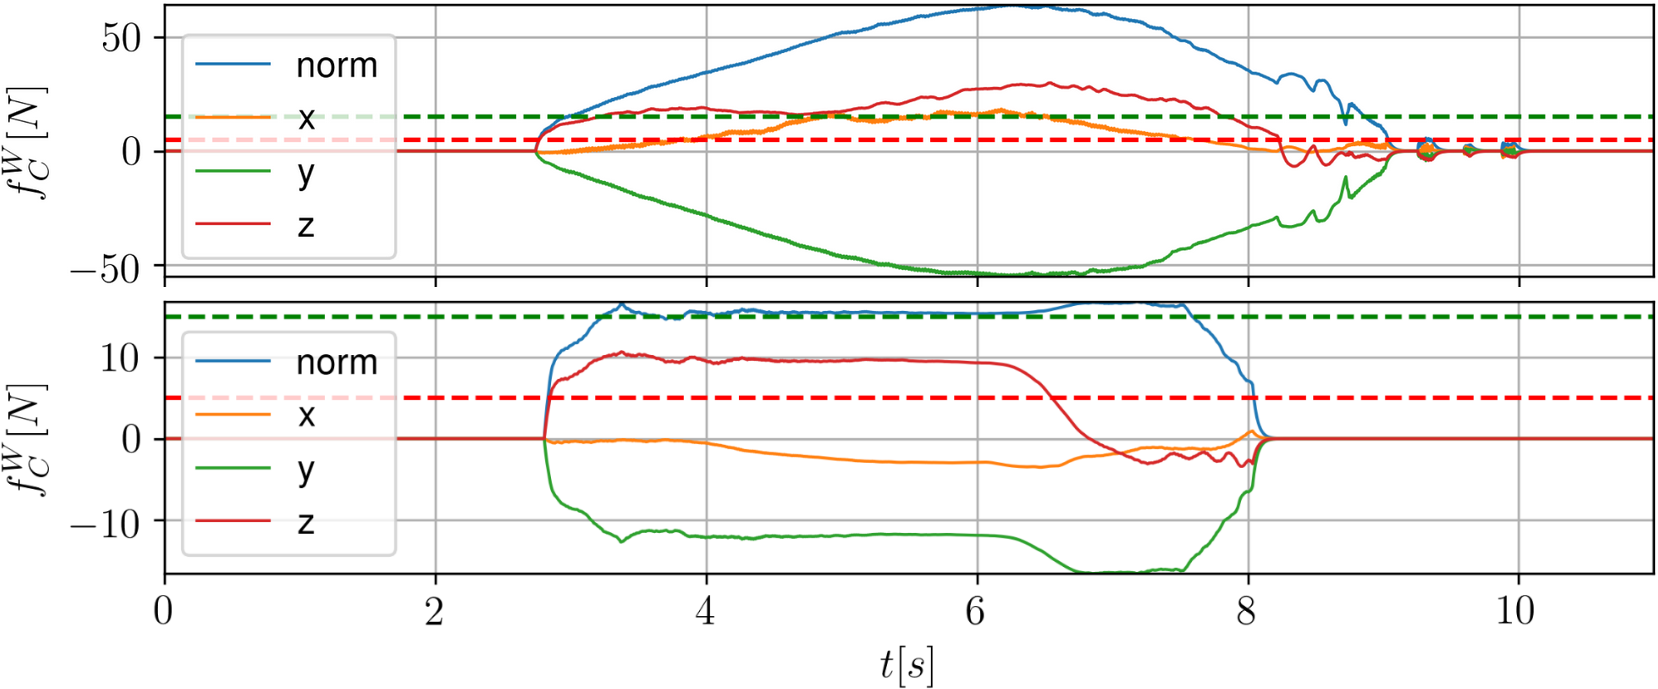
\includegraphics[width=0.98\linewidth]{figures/04_control/mug_placement_force.png}
\caption{ \textbf{mug placement task}. $x$, $y$, $z$ components and the norm of the contact force $f_W^C$. \textbf{Top}: the baseline controller without contact force upper bounds is shown in the top plot. \textbf{Bottom}: the contact-aware controller (\ref{eq:mpc_qp2}) with a modified end effector tracking objective. In both plots, the horizontal red dashed line represents $f_\text{threshold}$ and the green dashed line $\lambda_\text{max}$.}
\label{fig:mug_placement_damped_lsq_vs_ours}
\end{figure}

\subsubsection{Tracking error}
As shown in Fig. \ref{fig:mug_placement_tracking_error}, compared with the baseline, the contact-aware controller produces significantly less tracking error in the presence of external contact.

\begin{figure}
\vspace{-0.2cm}
\centering
\includegraphics[width=1.0\linewidth]{figures/04_control/mug_placement_tracking_error.pdf}
\caption{\textbf{mug placement task}. \textbf{Left}: position tracking error. \textbf{Right}: orientation tracking error. }
\vspace{-0.6cm}
\label{fig:mug_placement_tracking_error}
\end{figure}

\vspace{-0.1cm}
\subsection{Mug moving task (Fig. \ref{fig:experiments}b) \label{sec:mug_holding_results}} 
This task is defined by a joint-space trajectory $q_{\text{ref}}(t)$, with the goal of moving the mug along a straight line while keeping the mug orientation constant. The 16s trajectory $q_{\text{ref}}(t)$ is an interpolation between joint-space knot points obtained by inverse kinematics. As shown in Fig. \ref{fig:experiments}b, to move the mug to the desired destination, the robot needs to first establish a contact with the top face of the table, and then breaks contact with the side of the table.

The baseline we are comparing against is the class of controllers trying to achieve similar goals as ours but uses null-space projection, such as \cite{jorda2019contact}. As null-space projection cannot handle inequality constraints, the contact force upper bound is usually enforced by an equality constraint which sets the contact force to $\lambda_\text{max}$. When commanded to break contact by the reference trajectory, i.e.
\begin{equation}
\label{eq:break_away}
    J_u (q_\text{ref}^{l+1} - q^l) \leq 0,
\end{equation}
the contact force constraint needs to be abruptly removed in order to continue to track the reference trajectory \cite{jorda2019contact}. This can lead to large joint velocity during separation, as shown in Fig. \ref{fig:jorda_vs_ours}.

In contrast, the proposed QP controller does not explicitly make the decision to break contact based on (\ref{eq:break_away}), instead the break of contact comes naturally as a consequence of solving QP (\ref{eq:mpc_qp2}) with the inequality constraints on contact forces (\ref{eq:mpc_qp:force_upper_bound}). As shown in Fig. \ref{fig:jorda_vs_ours}, when the robot separates from the table, the drop in $\norm{f_W^C}$ occurs gradually with our QP controller, but abruptly with a null-projection-based controller.
\begin{figure}[h]
\vspace{-0.2cm}
\centering
\includegraphics[width=0.98\linewidth]{figures/04_control/ours_vs_jorda.pdf}
\caption{Comparison between our QP controller and null-space projection-based control in the \textbf{mug moving task}. \textbf{Top}: contact force norm $\norm{f_W^C}$. The red dashed line represents $f_\text{threshold}$ and the green dashed line $\lambda_\text{max}$. Both controllers can keep $\norm{f_W^C}$ near $\lambda_\text{max}$ when the robot is in contact. \textbf{Bottom}: robot joint velocity norm $\norm{v_q}$ during contact separation (from $t=10s$ to $t=14s$). Note the velocity spike in the null-space projection controller. In both plots, the solid lines are the mean of 10 runs; the shaded regions around the lines represent the maximum and minimum values of all runs.}
\label{fig:jorda_vs_ours}
\vspace{-0.7cm}
\end{figure}


\section{Conclusions}
We have presented a contact-aware controller that reconciles trajectory tracking with safety in unexpected contacts. The proposed controller is formulated as a QP with a quadratic cost on tracking error, a quasi-static model of the robot dynamics as constraints, and upper bounds on contact forces.

The tasks for hardware experiments are designed based on our vision of future motion planners: they are comprised of smooth, simple trajectories defined by only a few knot points. We have shown that the proposed controller is able to keep both the tracking error and contact forces small if the robot makes an accidental contact. In addition, our controller outperforms controllers based on null-space projection when an established contact needs to be broken as the robot follows a reference trajectory.

It is difficult to reliably sense more than one contacts on the arm from only joint torque \cite{pang2021identifying}. Nevertheless, with a more capable contact sensor such as \cite{luo2021learning}, we believe the proposed contact-aware controller will greatly reduce robots' reliance on environment sensing/monitoring and collision-free motion planning.
% \chapter{Tables}

\begin{table}
\caption{Armadillos}
\label{arm:table}
\begin{center}
\begin{tabular}{||l|l||}\hline
Armadillos & are \\\hline
our	   & friends \\\hline
\end{tabular}
\end{center}
\end{table}

\clearpage
\newpage

% \chapter{Figures}

\vspace*{-3in}

\begin{figure}
\vspace{2.4in}
\caption{Armadillo slaying lawyer.}
\label{arm:fig1}
\end{figure}
\clearpage
\newpage

\begin{figure}
\vspace{2.4in}
\caption{Armadillo eradicating national debt.}
\label{arm:fig2}
\end{figure}
\clearpage
\newpage

%% This defines the bibliography file (main.bib) and the bibliography style.
%% If you want to create a bibliography file by hand, change the contents of
%% this file to a `thebibliography' environment.  For more information 
%% see section 4.3 of the LaTeX manual.
\begin{singlespace}
\bibliography{main}
\bibliographystyle{unsrt}
\end{singlespace}

\end{document}

